% Prepared from the final Word manuscript, 7 November 2026.
% Official Springer Nature authoring class; pdfLaTeX; no line numbers.
\documentclass[pdflatex,sn-basic,Numbered]{sn-jnl}
\usepackage[T1]{fontenc}
\usepackage[utf8]{inputenc}
\usepackage{amsmath,amssymb,mathtools}
\usepackage{xcolor}
\usepackage{graphicx,longtable,booktabs,array,calc,multirow}
\usepackage{adjustbox}
\usepackage{microtype}
\usepackage{xurl}
\usepackage{fancyvrb}
\usepackage{caption}
\usepackage{placeins}
\usepackage{etoolbox}
\usepackage{bookmark}
\captionsetup{labelsep=space,labelfont=bf,font=small}
\captionsetup[figure]{name=Fig.}
\captionsetup[table]{name=Table}
\setcounter{secnumdepth}{3}
\setlength{\emergencystretch}{2em}
\urlstyle{same}
\hypersetup{hidelinks,pdftitle={Direct cognition problem: a semantic skeleton of mathematics and its growth},pdfauthor={Vasilii A. Gromov; Nikolai N. Evdokimov}}
\newcommand{\tightlist}{\setlength{\itemsep}{0pt}\setlength{\parskip}{0pt}}
\newcommand{\passthrough}[1]{#1}
\newsavebox{\displaybox}
\newcommand{\fitdisplay}[1]{\sbox{\displaybox}{$\displaystyle #1$}\ifdim\wd\displaybox>\linewidth\resizebox{\linewidth}{!}{\usebox{\displaybox}}\else\usebox{\displaybox}\fi}
\makeatletter
\newsavebox\pandoc@box
\newcommand*\pandocbounded[1]{\sbox\pandoc@box{#1}\ifdim\wd\pandoc@box>\linewidth\resizebox{\linewidth}{!}{\usebox\pandoc@box}\else\usebox\pandoc@box\fi}
\patchcmd\longtable{\par}{\if@noskipsec\mbox{}\fi\par}{}{}
\makeatother
\raggedbottom
\begin{document}
\title[A semantic skeleton of formal knowledge]{Direct cognition problem: a semantic skeleton of mathematics and its growth}
\subtitle{Epochs limit active premises while certificates preserve proofs}
\author[1]{\fnm{Vasilii A.} \sur{Gromov}}\email{stroller@rambler.ru}
\author*[1]{\fnm{Nikolai N.} \sur{Evdokimov}}\email{nevdokimov@hse.ru}
\affil[1]{\orgdiv{Laboratory for Semantic Analysis}, \orgname{National Research University Higher School of Economics}, \orgaddress{\street{11 Pokrovsky Bulvar}, \city{Moscow}, \postcode{109028}, \country{Russia}}}
\abstract{We study the direct cognition problem of formal knowledge: constructing a verifiable proof skeleton without a final target theorem under limited computational resources. We introduce a semantic skeleton of mathematics within a programme that distinguishes direct, inverse, and control cognition problems. Our continuous, generational generator separates a bounded active set, an archive of first proofs, and a library of closed fragments. The generator reversibly deactivates premises without deleting certificates. The selector measures how fragments shorten the expanded proof forest and accounts for definitions and overlaps; search need not activate stored fragments. An exponential lower bound on the number of explicitly expanded provable instances, together with a separate unboundedness result for the schema graph, limits exhaustive storage but does not imply that finite slices evade computation. A frozen panel of 144 source trajectories tests neutral continuation under resource guards. At its primary endpoint, learned half-selection with deferred replay increases mean novelty over ungated growth by 95.8\% and 30.3\% at propositional sizes 25 and 200, respectively, with eight positive pairs out of eight in each regime. A locked comparison across 16 sources and 963 human targets finds no confirmed adaptive advantage. The fixed extended repertoire initially covers 29 targets and averages 1.625 new common-residual targets at 90 operational processor-seconds. Network comparisons reveal modular structure and show how proof-edge conventions alter graph profiles. These results establish a certified method that preserves proofs and supports further growth, not a universal accelerator or an optimal skeleton.}
\keywords{formal knowledge, automated reasoning, semantic skeleton, proof hypergraph, theorem generation, Metamath}
\maketitle
\noindent\small ORCID (Nikolai N. Evdokimov): \url{https://orcid.org/0009-0003-3756-8281}\par\normalsize

\section*{1. Introduction}\label{introduction}
\addcontentsline{toc}{section}{1. Introduction}

Comparing the graph of all formally correct mathematical statements with the graph of those that humanity regards as theorems and lemmas \citep{MetamathSetMMPinned} reveals a striking difference (see Section 7.6). We call the latter object a semantic skeleton of mathematics. This article studies it and develops methods to generate it. This concept readily extends to any formalisable knowledge system, where we call it a semantic skeleton of formal knowledge. The skeleton provides a compact active representation through anchor statements and links to expandable proofs; it neither depicts the complete theorem space nor automatically discovers a system of mathematical concepts. Here, `semantic' means that the skeleton preserves formal statements, proof roles, and application conditions, whereas any substantive affinity with human mathematics requires a separate test. For knowledge-based reasoning, we ask which proved statements search should retain as premises under limited resources.

Our research programme distinguishes three cognition problems -- direct, inverse, and control cognition problems; this paper addresses the first. The \textbf{direct cognition problem} generates a proof skeleton without a final target theorem. We aim not merely to generate correct mathematical statements\footnote{Bachmair and Ganzinger \citep{BachmairGanzinger2001}, in \emph{Resolution Theorem Proving}, describe saturation through inference and redundancy criteria. Wernhard \citep{Wernhard2026}, in \emph{Generating Theorems by Generating Proof Structures}, studies target-free theorem generation. Section 2 distinguishes these foundations from the architecture and future-use test that we develop here.}, but to generate those that belong to the semantic skeleton. Ideally, we would rapidly generate statements that belong to the skeleton of mathematics (a formal system) on a personal computer, using interpretable AI. We would then, if necessary, seek further statements in the neighbourhood of a given skeleton vertex or vertices (``extend'' them), using, for example, non-interpretable (generative) AI; we leave this extension to future work. In the longer term, we aim to study the semantic skeleton of mathematics (and other formal systems) as a whole. \textbf{The inverse problem} takes a particular statement and seeks intermediate lemmas that connect it to the existing base (current skeleton), to certify its status relative to the chosen formal system. This requires a proof of the statement, a proof of its negation, or a separate independence argument; unsuccessful search returns unknown. The \textbf{control problem} selects a growth regime to obtain a graph with desirable properties such as modularity, concentrated reuse, or a particular degree distribution. Tuning towards an external structural objective belongs to control, and success on a target theorem belongs to the inverse problem; neither supplies evidence that a topology emerges spontaneously.

The present paper addresses the direct problem by generating a semantic skeleton of mathematics under a fixed computational budget. In particular, it examines how activating library fragments affects continuous forward growth from axioms. We assess three independent outcomes: (1) how many new canonical formulae the generator discovers, (2) how much reuse costs, and (3) how many results match human statements. Earlier checks measure how much of an exact finite benchmark the generator covers and how it continues from existing anchors; the skeleton's full return across a sequence of subsequent tasks remains a separate question.

The paper proposes (1) a formal contract, (2) an executable architecture, and (3) a reproducible comparison. The contract distinguishes proof status, activity, and certificate preservation, as well as schemata and their explicit instances\footnote{A formal contract states checkable guarantees (Definition 1). Proof status records whether a certificate passes the checker; activity permits use as a premise. A certificate records replayable proof steps. A schema contains expression variables; an instance substitutes admissible expressions consistently. Preserving a certificate retains its proof steps and dependencies.}. The architecture supports continuous generational growth through a bounded active set, reversible deactivation, and an append-only certificate log; it separates the fragment library from decisions to activate fragment conclusions as premises. The comparison separates proof preservation, shorter expanded representations, and productive subsequent search. Earlier tests of contextual transfer between branches motivate these distinctions, but the basic guarantees rely on standard proof-system properties: we claim no novelty when we infer forwards, combine strategies, or add provable lemmas.

The rest of the paper follows this structure. Section 2 relates the method to earlier research. Section 3 defines the proof representation and outcome criteria, and Section 4 establishes the limits of exhaustive explicit storage. Section 5 specifies the cumulative algorithm and lemma library. Sections 6 and 7 present the protocols, continuation results, and network comparison. Section 8 interprets these results, Section 9 answers the research question, and Section 10 explains how to reproduce the study. Appendices A--B, H, J, and K contain the proofs; the remaining appendices retain protocols, extended comparisons, and audit records.

\section*{2. Related papers}\label{related-papers}
\addcontentsline{toc}{section}{2. Related papers}

The problem connects automated theory exploration, inference control, and proof reuse. Four distinctions guide comparisons: whether a method generates a statement together with its proof or first proposes a conjecture; whether it receives a final target; what it excludes from computation; and how it measures usefulness. These distinctions carry more weight than the mere presence of a graph, queue, or lemma library.

\subsection*{2.1 Saturation and search-resource limits}\label{saturation-and-search-resource-limits}
\addcontentsline{toc}{subsection}{2.1 Saturation and search-resource limits}

Bachmair and Ganzinger \citep{BachmairGanzinger2001}, in their handbook chapter \emph{Resolution Theorem Proving}, explain how saturation combines inference rules with redundancy criteria. Schulz \citep{Schulz2002}, in \emph{E --- A Brainiac Theorem Prover}, and Kov\'{a}cs and Voronkov \citep{KovacsVoronkov2013}, in \emph{First-Order Theorem Proving and Vampire}, describe how clause indices, scores, and simplification direct that search. Target-free forward inference therefore supplies background rather than our novelty claim. We retain a long-lived archive of checked consequences and assess the skeleton through new growth under bounded activity.

Riazanov and Voronkov \citep{RiazanovVoronkov2003LRS}, in \emph{Limited Resource Strategy in Resolution Theorem Proving}, adapt permissible clause weights to remaining time and search statistics. Their strategy directly precedes resource-based pruning. Logical redundancy and low expected computational return support different guarantees: a suitable redundancy criterion can preserve completeness, whereas a heuristic return estimate need not. Our age-based pruning protects earlier certificates but does not ensure fair future enumeration.

Hoder and Voronkov \citep{HoderVoronkov2011}, in \emph{Sine Qua Non for Large Theory Reasoning}, reduce the initial theory for a particular problem through SInE. Blanchette and colleagues \citep{BlanchetteEtAl2016}, in \emph{A Learning-Based Fact Selector for Isabelle/HOL}, learn fact relevance from earlier proof dependencies. Jakub\r{u}v and Urban \citep{JakubuvUrban2017}, in \emph{ENIGMA: Efficient Learning-Based Inference Guiding Machine}, rank clauses during search according to how they contribute to successful proofs. These studies distinguish how a prover initially chooses premises from how it controls search. We additionally distinguish storing a fragment from admitting its conclusion to a bounded active slot, without labelling success against a final target.

\subsection*{2.2 Theory exploration and the usefulness of new statements}\label{theory-exploration-and-the-usefulness-of-new-statements}
\addcontentsline{toc}{subsection}{2.2 Theory exploration and the usefulness of new statements}

Colton \citep{Colton2002}, in his monograph \emph{Automated Theory Formation in Pure Mathematics}, develops automated concept and conjecture discovery. Smallbone and colleagues \citep{SmallboneEtAl2017}, in \emph{Quick Specifications for the Busy Programmer}, present QuickSpec, which enumerates terms, tests conjectural equalities, and reduces redundancy through their dependencies. Claessen and colleagues \citep{ClaessenEtAl2013}, in \emph{Automating Inductive Proofs Using Theory Exploration}, combine such exploration with inductive proof in HipSpec. These systems show how auxiliary statements can support later work; our archive instead accepts each statement together with its checked derivation.

Johansson and colleagues \citep{JohanssonEtAl2014}, in \emph{Hipster: Integrating Theory Exploration in a Proof Assistant}, validate conjectures through Isabelle/HOL and assess interestingness against ordinary and stronger proof mechanisms. Singher and Itzhaky \citep{SingherItzhaky2021}, in \emph{Theory Exploration Powered by Deductive Synthesis}, combine symbolic enumeration, rewriting, congruence closure, and inductive checking in TheSy. Their bounded solver also examines mutual derivability. These studies motivate separate measures of novelty, proof status, and usefulness; our archive checks every accepted derivation, whereas our experiments assess continued growth rather than mutual derivability of complete theories.

McCasland, Bundy, and Smith \citep{McCaslandBundySmith2017}, in MATHsAiD: Automated mathematical theory exploration, describe theorem discovery from supplied axioms and definitions and distinguish it from proving a supplied goal. This distinction also frames our direct problem. We distinguish archived certificates, reusable fragments, and active premises in our experiments, and measure how much continued generation costs.

\subsection*{2.3 Generating proof structures: the closest predecessors}\label{generating-proof-structures-the-closest-predecessors}
\addcontentsline{toc}{subsection}{2.3 Generating proof structures: the closest predecessors}

Wernhard and Bibel \citep{WernhardBibel2024}, in \emph{Investigations into Proof Structures}, distinguish proof-tree size from minimal directed acyclic proof-graph size and study level-wise enumeration, theorem-size bounds, and bounded caches. Their analysis directly informs our generator. We extend the experimental focus to persistent certified growth and separately control archived proofs, reusable fragments, and active premises.

Wernhard \citep{Wernhard2026}, in \emph{Generating Theorems by Generating Proof Structures}, combines target-free enumeration, inductive levels, lemma synthesis through shorter proof representations, and comparison with human Metamath theorems. We build on this methodological precedent through continuous certified growth, reversible activity control, and prospective leases whose costs we measure. Our comparisons separate fragment recurrence from additional output when search admits fragment conclusions.

Rawson and colleagues \citep{RawsonEtAl2023}, in \emph{Lemmas: Generation, Selection, Application}, separate those three stages and compare structural usefulness scores with changes in proving work after lemma addition. Their tests motivate our distinction between shorter proof code and faster subsequent search. They assess lemmas through proof tasks; our principal trajectories instead continue without an external final target.

Wernhard and Zombori \citep{WernhardZombori2025}, in their preprint \emph{Mathematical Knowledge Bases as Grammar-Compressed Proof Terms: Exploring Metamath Proof Structures}, encode libraries through compressed proof terms, including parametrised fragments. Our code-length criterion scores particular closed first proofs, whereas a separate compiler derives general closed schemata from open modus-ponens programmes. The archive already shares subproofs. Consequently, shorter expanded forests measure the declared proof-term code rather than additional compression of the archive graph or universal human lemma value.

\subsection*{2.4 Acquired knowledge: from recurrence to computational return}\label{acquired-knowledge-from-recurrence-to-computational-return}
\addcontentsline{toc}{subsection}{2.4 Acquired knowledge: from recurrence to computational return}

Minton \citep{Minton1990Utility}, in \emph{Quantitative Results Concerning the Utility of Explanation-Based Learning}, measures how applicability checks and maintenance can outweigh gains from acquired knowledge. Our setting adds competition for a bounded number of active-premise slots. Frequent fragment occurrences establish reuse, but only a costed continuation test can assess whether access to those conclusions yields more new results. We therefore report code-length savings separately from computational return.

Kaliszyk and Urban \citep{KaliszykUrban2015}, in \emph{Learning-Assisted Theorem Proving with Millions of Lemmas}, select intermediate lemmas through acquisition cost, reuse, centrality, and greedy changes to the dependency graph. They also distinguish protocols by access to future proofs. Our selector recalculates overlaps using only the preceding forest, because earlier choices change the value of another fragment. After a run, we separately measure how many human statements the results cover; this diagnostic does not supply an independent holdout.

\subsection*{2.5 Trainable generators and growing libraries}\label{trainable-generators-and-growing-libraries}
\addcontentsline{toc}{subsection}{2.5 Trainable generators and growing libraries}

Wang and colleagues \citep{WangEtAl2023Lego}, in \emph{LEGO-Prover: Neural Theorem Proving with Growing Libraries}, build and reuse verified auxiliary skills while solving formal tasks. Yang and colleagues \citep{YangEtAl2023}, in \emph{LeanDojo: Theorem Proving with Retrieval-Augmented Language Models}, combine premise retrieval with search and track fact availability. These systems inform future uses of a skeleton for target-driven reasoning. Our historical direct-growth panels start from axioms, whereas the native extensions inherit a certified source library. Neither calls a language model for formulae or fragments.

Poesia and colleagues \citep{PoesiaEtAl2024}, in \emph{Learning Formal Mathematics from Intrinsic Motivation}, jointly learn conjecturing and proving in MINIMO from an initial axiomatisation. Ota and colleagues \citep{OtaEtAl2026}, in their preprint \emph{Self-Supervised Theorem Discovery in a Formal Axiomatic System}, turn discovered theorems into prover actions and select them through generalisation and difficulty of rediscovery. Both systems create their own search targets. Our generator instead continues forward without a trainable target-setting loop.

Lin and colleagues \citep{LinEtAl2024}, in \emph{ATG: Benchmarking Automated Theorem Generation for Generative Language Models}, assess generated theorems partly through their usefulness for subsequent proving. We test neutral direct continuation and exact matches to human statements. This choice measures further target-free growth; independent goal-directed tasks would test the complementary inverse problem.

\subsection*{2.6 Prover cooperation and graphs of mathematical libraries}\label{prover-cooperation-and-graphs-of-mathematical-libraries}
\addcontentsline{toc}{subsection}{2.6 Prover cooperation and graphs of mathematical libraries}

Urban \citep{Urban2013BliStr}, in \emph{BliStr: The Blind Strategymaker}, constructs search-strategy portfolios automatically. Bonacina and Hsiang \citep{BonacinaHsiang1995}, in \emph{The Clause-Diffusion Methodology for Distributed Deduction}, distribute inferences and data across processes. Denzinger and Fuchs \citep{DenzingerFuchs1999}, in \emph{Cooperation of Heterogeneous Provers}, select outgoing and incoming clauses according to recipient capabilities. These precedents motivate context-dependent exchange rather than a novelty claim for parallel growth itself. Appendices C--E and I retain our exchange and multibranch outcomes, including losses.

Tomaszuk and colleagues \citep{TomaszukEtAl2023}, in \emph{MMLKG: Knowledge Graph for Mathematical Definitions, Statements and Proofs}, represent the existing Mizar library as a knowledge graph. Li and colleagues \citep{LiEtAl2026}, in their preprint \emph{The Network Structure of Mathlib}, distinguish dependency levels and relate observed centrality to formalisation infrastructure. These studies motivate a graph-level account of mathematical libraries. Our generator additionally requires joint premises and expandable certificates; high degree, short paths, or a compact projection cannot replace those proof conditions.

\subsection*{2.7 Position of this work}\label{position-of-this-work}
\addcontentsline{toc}{subsection}{2.7 Position of this work}

Our method assigns each proven formula three distinct roles: an archived result, a reusable library entry, and a possible active premise. Certificate replay checks the first role, past savings in proof code help select reusable entries, and neutral continuation measures future use. Structural synthesis adds another route to library entries through checked deduction. The contribution combines these mechanisms with explicit access permissions and tests their incremental effects over fixed controls.

\section*{3 Formal model and outcome criteria}\label{formal-model-and-outcome-criteria}
\addcontentsline{toc}{section}{3 Formal model and outcome criteria}

\subsection*{3.1 Calculus and proof state}\label{calculus-and-proof-state}
\addcontentsline{toc}{subsection}{3.1 Calculus and proof state}

A proof certificate records elementary inferences and substitutions that a checker can replay from the initial base. We call a statement proven once its certificate passes those checks, and active when the generator may use it as a premise. A schema contains variables that stand for admissible expressions; an instance replaces those variables consistently. A configuration fixes the language, proof rules, and contextual requirements:

\[\fitdisplay{\mathcal{C} = (\Sigma,\Gamma,\Re,\nu,\Xi),}\]

where \(\Sigma\) specifies the language, \(\Gamma\) denotes the initial axioms or schemata, \(\Re\) contains the rules, \(\nu\) maps each statement to its declared canonical form, and \(\Xi\) describes contextual restrictions. In systems with quantifiers and hypotheses, each vertex includes the necessary context, variable types, and admissible-substitution conditions alongside its formula. Formula identity alone therefore need not identify the full proof state.

A typed hypergraph\footnote{A typed directed hypergraph records statements as vertices, together with their variable types, hypotheses, and side conditions. A directed hyperedge joins an ordered group of premises to one conclusion and records the rule and substitution. Its premise order identifies rule roles; the inference requires those premises jointly.

  For modus ponens (MP), the minor premise \(p\) and major premise \(p \rightarrow q\) jointly yield \(q\); neither premise alone supplies that inference.} \(H = (V,E)\) provides the primary representation. We record a rule application as

\[\fitdisplay{e = (p_{1},\ldots,p_{k};\rho;\sigma;\chi;q),}\]

where \(p_{i}\) denotes premises in role order, \(\rho\) denotes the rule, \(\sigma\) denotes the substitution, \(\chi\) contains side conditions, and \(q\) denotes the conclusion. Each hyperedge requires all its premises jointly, whereas alternative hyperedges represent different derivations of the same conclusion. The representation thus preserves the distinction between jointly necessary premises and alternative proofs.

To canonicalise means to remove only the declared redundancy of notation. In the implicational fragment, the procedure normalises variable names by first occurrence without identifying arbitrary logically equivalent formulae. A canonical identifier therefore does not turn a vertex into a semantic equivalence class.

\subsection*{3.2 Skeleton contract}\label{skeleton-contract}
\addcontentsline{toc}{subsection}{3.2 Skeleton contract}

\textbf{Definition 1.} A certified proof skeleton consists of a triple

\[\fitdisplay{\mathcal{S} = (S,\Omega,\mathsf{E}\mathsf{x}\mathsf{p}\mathsf{a}\mathsf{n}\mathsf{d}),}\]

with the following properties. A finite certificate in \(\Omega\) supports every anchor vertex \(v \in S\); certificate dependencies satisfy well-foundedness; \(\mathsf{E}\mathsf{x}\mathsf{p}\mathsf{a}\mathsf{n}\mathsf{d}\) expands an anchor-lemma reference into a proof from the permitted initial base; and every elementary step passes rule and side-condition checks. Together, these requirements let a checker recover each anchor independently from that base.

The contract does not require every known alternative proof. An implementation may preserve one correct witness, several variants with different costs, or a common structure that shares subproofs. Deleting the sole expandable witness nevertheless violates the contract unless another certified reconstruction remains available.

`Semantic' carries a restricted operational meaning here. The skeleton preserves formal statements, their proof roles, and application conditions, whereas we must test separately whether the skeleton resembles how humans organise mathematics. In particular, provable equivalence among all theorems relative to a common theory provides too coarse a relation for identifying useful anchor lemmas.

\subsection*{3.3 Reconstruction and new growth}\label{reconstruction-and-new-growth}
\addcontentsline{toc}{subsection}{3.3 Reconstruction and new growth}

Proof expansion and new growth serve distinct purposes:

\[\fitdisplay{\mathsf{E}\mathsf{x}\mathsf{p}\mathsf{a}\mathsf{n}\mathsf{d}(\mathcal{S},v) \rightarrow \pi_{v},\quad\quad\mathsf{G}\mathsf{r}\mathsf{o}\mathsf{w}(\mathcal{S},b) \rightarrow \Omega_{b}.}\]

The first operator returns a certificate for an existing anchor. The second performs forward inference under budget \(b\) without a final target formula, using the initial axioms, selected anchors, and its own new consequences. Vertices that serve only as proof support do not automatically enter the available premise set, so archival presence alone does not confer search activity.

New-growth counts exclude rediscovery of formulae that the archive already contains. Let \(\Omega_{0}\) denote the common initial archive from which the comparison policies choose anchors, and define the main direct-continuation measure as

\[\fitdisplay{N_{b}(\mathcal{S} \mid \Omega_{0}) = \left| V(\Omega_{b})\setminus V(\Omega_{0}) \right|.}\]

This measure counts syntactic novelty under the declared canonicalisation, even after earlier formulae leave the active skeleton. It does not establish mathematical significance for every new result.

An external set \(T\) supplies a supplementary measure of new exact matches:

\[\fitdisplay{M_{b}(\mathcal{S},T \mid \Omega_{0}) = \left| T \cap (V(\Omega_{b})\setminus V(\Omega_{0})) \right|.}\]

Earlier experiments in Appendices D--E separately recorded coverage through one-way substitution, requiring each human statement to instantiate a discovered schema. This test neither unifies both sides through changes to each nor launches a new proof search. Exact and substitution-coverage increments use different baselines and do not add together; for the historical 48-trajectory activity series, we calculate only exact human matches.

The later native tests use typed one-way coverage with mandatory distinct-variable conditions. For source block \(j\), let \(T\) denote the external reference and let \(C_{T}(S_{j,m},0)\) denote the statements that method \(m\) covers before further search. We freeze a common residual

\[\fitdisplay{R_{j} = T\setminus \bigcup_{m}C_{T}(S_{j,m},0),\quad\quad Q_{j}(m,h) = \left| R_{j} \cap C_{T}(S_{j,m},h) \right|.}\]

The observer measures coverage of committed results; it supplies no premise, reward, or proposed conclusion. The residual removes every method's initial coverage advantage within a block. Counts of \(Q_{j}\) test new reference capability, whereas \(N_{b}\) counts syntactically new formulae outside the common archive. Neither measure substitutes for the other, and exact matches remain a separate readout.

The operator \(\mathsf{S}\mathsf{e}\mathsf{a}\mathsf{r}\mathsf{c}\mathsf{h}(\mathcal{S},\tau,b)\) belongs to the inverse problem because it receives a target formula \(\tau\). Its solvability and cost could inform future skeleton assessment alongside the present forward measures. They do not replace the test of \(\mathsf{G}\mathsf{r}\mathsf{o}\mathsf{w}\) that this paper performs.

Resource accounting distinguishes the active set and reserve from the library, proof support, and archive. We measure their sizes separately, together with peak memory for the entire process; a fixed premise count does not imply fixed total memory. The principal size bounds \(L = 25,200\) count every syntax-tree vertex, not only leaves, and therefore constrain a different quantity from the active-set limit.

\subsection*{3.4 Useful skeletons and empirical Pareto sets}\label{useful-skeletons-and-empirical-pareto-sets}
\addcontentsline{toc}{subsection}{3.4 Useful skeletons and empirical Pareto sets}

A useful skeleton preserves checked proofs and supports further inference within the declared budget. The proof requirements guarantee the first property; neutral continuation tests the second. This operational criterion links proof preservation to the work that the retained library supports.

For each policy and anchor cap, we record a triple: the measured cost of constructing and using a skeleton, the bytes in its proof-backed package, and the new schemata that it generates during continuation. One setting dominates another only when it uses no more CPU or package bytes, yields at least as many new schemata, and improves at least one coordinate. The empirical Pareto set contains the nondominated settings within the declared finite comparison grid. This definition avoids assigning an arbitrary exchange rate between a byte, a CPU-second, and a new formula.

We compare settings only within one logic--size regime, one source ceiling, one continuation horizon, and a common exclusion archive. Package bytes include both anchors and certificate support; an anchor count alone omits that support. A frontier of sample means describes the observed trade-offs, whereas paired outcomes show whether individual schedules share them. Neither frontier establishes a population optimum, and changing the continuation horizon changes the quality coordinate rather than merely extending the same cost axis.

\section*{4 Limits of exhaustive explicit construction}\label{limits-of-exhaustive-explicit-construction}
\addcontentsline{toc}{section}{4 Limits of exhaustive explicit construction}

The combinatorial argument depends on the unit of storage. Let \(T_{L}\) contain the syntactically distinct formulae over one fixed letter \(p\) that admit proofs in which every formula, including axiom instances, contains at most \(L\) syntax-tree vertices. Size counts syntax-tree vertices, and the calculus contains the schemata \(K:A \rightarrow (B \rightarrow A)\) and \(S:\lbrack A \rightarrow (B \rightarrow C)\rbrack \rightarrow \lbrack(A \rightarrow B) \rightarrow (A \rightarrow C)\rbrack\), together with modus ponens. The resulting bound concerns explicit formula instances under these conventions.

\textbf{Theorem 1.} For every integer \(m \geq 0\),

\[\fitdisplay{|T_{18m + 17}| \geq {Cat}_{m},\quad\quad{Cat}_{m} = \frac{1}{m + 1}\binom{2m}{m} \sim \frac{4^{m}}{\sqrt{\pi}\, m^{3/2}}.}\]

These conclusions contain \(4m + 3\) syntax-tree vertices and admit proofs with at most two applications of modus ponens along any path from an axiom instance. Appendix A presents the full proof and intermediate size calculations, using standard Catalan enumeration \citep{FlajoletSedgewick2009}.

Exhaustive representation with a separate record for each such formula requires exponentially many records in \(L\). No fixed total capacity can accommodate that representation for every increasing \(L\). This output-volume bound does not supply a new lower bound on the complexity of finding a single proof, and it permits streaming output, growing storage, and exhaustive computation of any fixed finite slice.

The generator needs a separate schema-level bound. Every \(F \rightarrow F\) instantiates the single schema \(A \rightarrow A\), so the explicit family behind Theorem 1 collapses under schema storage. Its exponential bound therefore \textbf{does not transfer} to the number of canonical schemata in the archive.

\textbf{Theorem 2.} Let \(H_{d}^{sch}\) contain \(K\) and every most general result of schematic modus ponens up to depth \(d\), with separate renaming of premise variables and canonicalisation only up to renaming. With no size or width limits, subsumption, or pruning,

\[\fitdisplay{|V(H_{d}^{sch})| \geq d + 1.}\]

Appendix A proves the claim. Together, the bounds establish why an ever-growing exact graph eventually exceeds fixed retained capacity, distinguishing explicit instances from canonical schemata. They motivate a design that limits active work and preserves proof certificates separately. Appendix A details the assumptions, pair counts, and finite restrictions.

\section*{5 Continuous skeleton and proof library}\label{continuous-skeleton-and-proof-library}
\addcontentsline{toc}{section}{5 Continuous skeleton and proof library}

\subsection*{5.1 Continuous growth with distinct states}\label{continuous-growth-with-distinct-states}
\addcontentsline{toc}{subsection}{5.1 Continuous growth with distinct states}

The continuous variant keeps one generator across epochs and reserves no compulsory time share for a second branch. We track its state as

\[\fitdisplay{X_{e} = (A_{e},P_{e},D_{e},\Omega_{e},\mathcal{I}_{e},B_{e}),}\]

where \(A_{e}\) contains active premises, \(P_{e}\) holds the passive queue of proven candidates, \(\Omega_{e}\) contains the certificate archive, \(\mathcal{I}_{e}\) contains working indices, \(B_{e}\) denotes remaining resources, and \(D_{e}\) contains root identifiers for closed library fragments whose certificates reside in \(\Omega_{e}\). The program defines retained anchors as \(S_{e} = A_{e} \cup D_{e}\), without an additional independent state component. The two sets serve distinct purposes: \(A_{e}\) supplies search premises, whereas \(D_{e}\) stores references to multistep proofs that the checker verified. Their ancestor proof support \(Anc(A_{e} \cup D_{e})\) serves checking and expansion, not an additional active base.

The archive grows through new canonical statements and their first proofs. The historical generational implementation records certificate increments and state snapshots, with checksums and links to preceding receipts. An independent checker reconstructs the axioms and elementary rules and checks canonical uniqueness and topological order. The native implementation instead exports complete checkpoints at source and interface boundaries, together with future-admission and rediscovery logs. Both preserve earlier certificates, but their storage costs differ. Checksums test integrity against fixed records rather than authenticate authorship.

With an append-only log, the program avoids serialising the same archive prefix repeatedly. If \(n_{e}\) counts archive records after epoch \(e\), full-prefix storage writes \(\sum_{e}^{}n_{e}\) records, whereas the append-only log writes \(n_{E}\) records over \(E\) epochs. This exact difference concerns repeated serialisation along the same trajectory, not overall acceleration: working-state snapshots require separate storage, and construction, checking, and indexing also take time.

Only the initial axioms receive permanent protection in the working set. The policy retains other active formulae for finite periods and extends those periods when a formula contributes to the first proof of a new result; library-selected formulae receive a separate finite period. Deactivation removes a formula from search indices but preserves its archive entry. If search rediscovers that formula, the policy can return it to the passive queue after a specified delay and within a return quota, measuring its new age from queue re-entry rather than old proof depth. These operations neither change the certificate nor turn a derived lemma into an axiom.

Explicit limits constrain active derived formulae and passive candidates after every layer. The policy first preserves the new search frontier, then accounts for finite library-retention periods and recent productive use. Per-layer selection width and total active-set size remain separate parameters. Since the archive retains every entry, bounded activity does not imply constant total memory.

\subsection*{5.2 Utility of a reusable proof fragment}\label{utility-of-a-reusable-proof-fragment}
\addcontentsline{toc}{subsection}{5.2 Utility of a reusable proof fragment}

A closed fragment represents a particular first proof of a lemma with initial axioms at its leaves. Closure excludes unproven open premises, not schema variables; expansion follows each internal vertex's archived premises in their original order. This coding stage names existing proofs. The separate structural compiler below generalises short open proof programmes and derives their closed implication schemata. Both routes retain elementary certificates and leave the original consequence relation unchanged.

Fragment cost accounts for repeated premise positions. Let \(R_{e}\) denote a finite set of recent proofs for selection, and let \(pa(v)\) denote the ordered parent list of vertex \(v\), allowing repeated entries. Counting each premise occurrence with its multiplicity gives the expanded proof-term size

\[\fitdisplay{t(v) = 1 + \sum_{p \in pa(v)}^{}t(p).}\]

The unit counts an axiom name, a rule application, or a fragment reference. For a chosen library \(D\), define

\[\fitdisplay{c_{D}(v) = \left\{ \begin{matrix}
1, & v \in D, \\
1 + \sum_{p \in pa(v)}^{}c_{D}(p), & v \notin D,
\end{matrix} \right.\ }\]

\[\fitdisplay{d_{D}(v) = 2 + \sum_{p \in pa(v)}^{}c_{D}(p).}\]

The quantity \(d_{D}(v)\) includes a definition header and its root instruction, whereas references to other definitions must follow the original well-founded dependencies. Thus the encoding gain for the proof forest accounts for both references and definitions:

\[\fitdisplay{G(D;R_{e}) = \sum_{v \in R_{e}}^{}t(v) - \left\lbrack \sum_{v \in R_{e}}^{}c_{D}(v) + \sum_{v \in D}^{}d_{D}(v) \right\rbrack.}\]

The selector admits fragments only while they reduce code length; it need not fill its quota. Candidates comprise multistep proofs of height at least two that occur at least twice in the expanded forest; a bounded pool ranks them by how much each could reduce repetition. The greedy selector then adds the fragment with the largest positive increment in \(G\) and recalculates overlaps. The selector stops when no positive increment remains, so the procedure searches only a bounded candidate pool and does not guarantee optimal compression.

\textbf{Lemma 1 (library expansion).} For a finite acyclic archive, this encoding expands into the original forest of first proofs. If selection starts from an empty library and admits only strictly positive increments in \(G\), its final gain on the training forest remains non-negative. Appendix B.5 proves the lemma.

The lemma certifies exact recovery of the original proofs and a non-negative code-length gain on the selection forest. The gain \(G\) measures savings in expanded proof-term symbols; the archive already shares identical subproofs. The continuation experiments separately measure whether library conclusions improve future search under a CPU budget.

Transfer tests freeze \(D_{e}\) before the next layer. We then count how often new first proofs use library conclusions directly and how much fragment references shorten expanded terms; building definitions and selecting fragments both consume the CPU budget. We report reference counts inside the expanded tree separately from immediate premise uses, because one immediate reference can stand for many repeated subtrees.

\subsection*{5.3 Library storage and premise activation}\label{library-storage-and-premise-activation}
\addcontentsline{toc}{subsection}{5.3 Library storage and premise activation}

Two treatments apply the same fragment-selection procedure but differ in their influence on search. In the active variant, a selected conclusion receives finite retention and, when necessary, returns to the active set while occupying an ordinary slot in the layer width. In the passive variant, the program stores and checks the library without changing indices, the queue, retention periods, or generator premises. At equal completed-epoch counts, the passive search trajectory therefore matches the no-library variant, although maintenance cost and the epoch that search reaches within a CPU budget may differ.

This separation tests whether an effect arises from library maintenance or a change in search context. Only the active treatment may alter that context. These two treatments do not establish the causal benefit of each fragment, which would require matched local interventions from an identical preceding state.

\subsection*{5.4 Continuous construction cycle}\label{continuous-construction-cycle}
\addcontentsline{toc}{subsection}{5.4 Continuous construction cycle}

A generation denotes a layer of new consequences, whereas an epoch denotes a point at which the program updates search state. Epoch number does not equal minimum proof height from the initial axioms. Unlike earlier restarts from selected anchors, this algorithm preserves one generator and its unfinished work; the experimental protocol specifies the retention periods, quotas, and bounds that govern that continuity.

\textbf{Algorithm 1. Continuous certified growth.}

\begin{enumerate}
\def\labelenumi{\arabic{enumi}.}
\tightlist
\item
  Check the initial axioms or inherited certified library, create the working indices, and initialise the archive and reusable dictionary.
\item
  While resources permit another layer, select an admissible frontier from the queue according to the fixed policy and its tie-breaking rule.
\item
  Process available rule applications. Check substitutions and side conditions, and canonicalise conclusions. Store a first proof for each new formula; handle rediscovery separately without increasing the new-formula count.
\item
  Update productive-use records and finite retention periods. Apply active-set and queue bounds while preserving certificates for inactive formulae. Return eligible rediscoveries to the queue subject to the specified delay and quota.
\item
  At the designated epochs, select a library from the preceding proof forest. In the active variant, apply bounded retention to its conclusions; in the passive variant, leave search state unchanged.
\item
  Store the new certificate increment and state snapshot. Credit only a fully completed layer within budget, and record the stopping reason.
\end{enumerate}

At a library-review point, the structural extension may add checked lemma schemata before the upper codec runs. It preserves the preceding interface and charges new definitions; it does not replace the accumulated generator with a new search from a hand-picked theorem list. Historical generational panels commit complete layers, whereas native continuations charge individual primitive attempts and exclude any result that completes after a horizon. Each protocol fixes its own accounting boundary before the run.

Epochs limit active premises while certificates preserve proofs.

The algorithmic budget includes fragment selection, index updates, internal checking, and storage. The independent checker replays the complete log after the experiment; we account for its cost separately. The pseudocode consequently specifies dependency order among operations, not equal execution times for successive layers.

\subsection*{5.5 Soundness and the limit of the guarantee}\label{soundness-and-the-limit-of-the-guarantee}
\addcontentsline{toc}{subsection}{5.5 Soundness and the limit of the guarantee}

Every archive certificate expands to the initial base provided the axioms satisfy the configuration, each new step passes checking, and each reference points to an earlier certified vertex. Appendices B.1--B.2 state the formal guarantees and prove them. These guarantees preserve existing proofs when the policy deactivates premises, but do not ensure complete enumeration: an inactive premise can prevent a useful future rule application.

Adding a provable lemma does not strengthen the underlying logic, but can change which proofs the available resources can reach \citep{CookReckhow1979}. Under size and height bounds, we must account explicitly for intermediate formulae when we expand proofs; Appendix B and Section G.1 provide the full resource conditions and a specific identity example. Complete finite saturation additionally requires fair processing of every rule application that becomes available, a guarantee that the present bounded policy does not establish.

\subsection*{5.6 Learned pair selection with deferred replay}\label{learned-pair-selection-with-deferred-replay}
\addcontentsline{toc}{subsection}{5.6 Learned pair selection with deferred replay}

The later variant controls pairs of candidate premises before it unifies them. A frozen model scores only premise syntax and existing first-proof heights; it never inspects a proposed conclusion. Its training labels mark first-proof ancestry that supports an earlier compression dictionary. The policy retains roughly half of compatible candidates, includes a fixed exploratory share, and preserves their production traversal order. Thus it predicts a corridor towards useful proof support rather than the truth of an unseen theorem.

Deferred replay retains some skipped pairs in a bounded queue. Each epoch can test up to 128 ready pairs and reserve up to four ordinary premise slots to restore missing parents. A replay uses only currently active, certified premises; it does not introduce a new axiom or activate cold proof support. Queue capacity, overflow, and the cost of scores remain explicit. This mechanism delays the point at which the hard filter saturates while preserving the same elementary proof checker.

The policy constructs an archive, then extracts proof-backed anchor packages for neutral continuation. Source work, package choice, and continuation enter the reported chain CPU cost. Training and the later independent audit enter separate accounts. Code-length gain chooses candidate support, and continued growth measures operational usefulness. These separate tests allow a compact package to succeed without claiming that every retained formula belongs to a unique mathematical core.

\subsection*{5.7 Additional compression above the accumulated library}\label{additional-compression-above-the-accumulated-library}
\addcontentsline{toc}{subsection}{5.7 Additional compression above the accumulated library}

The upper codec preserves a base dictionary \(D_{0}\) and adds a definition only when its joint marginal gain remains positive. It recalculates nested references and definition costs after each addition and imposes no target dictionary size. For an eligible fragment, let \(r\) count its expanded occurrences in the current forest and dictionary bodies, and let \(b\) count the symbols in its current body. The exact saving under this code equals

\[\fitdisplay{\Delta(v \mid D) = (r - 1)(b - 1) - 2.}\]

The two charged symbols account for a new definition's root and header after the reference savings. Appendix K.1 proves this identity and its telescoping guarantee. Positive increments improve the previous encoding, even when \(D_{0}\) already contains mandatory entries; they do not guarantee a globally shortest code, fewer archive bytes, or faster future inference.

\subsection*{5.8 Structural synthesis of general lemma schemata}\label{structural-synthesis-of-general-lemma-schemata}
\addcontentsline{toc}{subsection}{5.8 Structural synthesis of general lemma schemata}

The structural layer abstracts a short MP proof tree, replaces its boundary by hypotheses, and considers possible equalities among those hypotheses. Joint typed unification solves all MP constraints together. For each consistent programme and order of its distinct boundary hypotheses, the compiler applies the deduction theorem and derives a closed implication schema. The generalisation rule (Gen) cuts an open fragment: the compiler never moves a deduction step through unrestricted Gen.

For example, a programme with boundary \(p\), \(p \rightarrow q\), and \(q \rightarrow r\) concludes \(r\). An appropriate discharge order yields

\[\fitdisplay{(p \rightarrow q) \rightarrow \left( (q \rightarrow r) \rightarrow (p \rightarrow r) \right).}\]

The compiler recovers this familiar composition law without a human theorem target. It expands every new step through ax-1, ax-2, and ax-mp, or invokes an existing checked schema through an explicit admissible instance. All output certificates pass the native checker and the independent Metamath verifier. Proposition K.2 states the proof obligation; this compiler implements the standard deduction construction rather than a new deduction theorem.

The catalogue distinguishes a requested principal formula from the actual schema that its certificate supplies. A more general stored schema may cover several requests, so we deduplicate delivered statements and their applicability frames. This distinction explains why candidate counts and delivered-rule counts need not coincide. The finite grammar and size guards bound the actual construction, not all possible useful lemmas.

\subsection*{5.9 Fixed structural repertoire}\label{fixed-structural-repertoire}
\addcontentsline{toc}{subsection}{5.9 Fixed structural repertoire}

The final native architecture combines the cumulative constructor and positive-marginal codec with a finite structural repertoire. A common grammar delivers 217 checked schemata through three open MP nodes, including 16 short outputs through two nodes. The fixed quota-matched variant adds 12 extended outputs that the fixed ranking selects using pooled earlier development profiles. It uses no held-out theorem to select those rules. This fixed repertoire supplies a reproducible working configuration, not an optimum over all possible libraries.

The locked comparison separately tests whether the source history should change those 12 outputs, versus fixed, random, and whole-catalogue alternatives. The adaptive score belongs to that comparative experiment rather than the recommended architecture. Appendix K.6 specifies it fully, and the results retain its registered outcome.

\subsection*{5.10 Search permissions after the library freezes}\label{search-permissions-after-the-library-freezes}
\addcontentsline{toc}{subsection}{5.10 Search permissions after the library freezes}

The neutral test receives only declared interface statements as premises. It cannot use certificate-only support for sampling, subsumption, or rejecting a rediscovery as already known. If search derives a hidden support statement again, the checker first validates a new witness from currently permitted parents; only then does the statement gain search rights. A separate log retains that witness even when the old archive already stores the same statement.

The neutral continuers reset learned scores, deferred queues, and reuse counters. They apply either uniform premise sampling or the same fixed mixture of uniform, bridging, contracting, and frontier sampling to every arm. They retain admitted future results without the constructor's rot-pruning or active cap. Thus this test assesses a library's use under a common engine, not the effect of running each builder's controller longer. The mixed engine retains an identifier-dependent frontier preference, so the experiment concerns delivered representations rather than an invariant semantic functional.

\section*{6 Materials and methods}\label{materials-and-methods}
\addcontentsline{toc}{section}{6 Materials and methods}

\subsection*{6.1 Formal systems and the scope of the tests}\label{formal-systems-and-the-scope-of-the-tests}
\addcontentsline{toc}{subsection}{6.1 Formal systems and the scope of the tests}

The historical propositional panels use \(\rightarrow ,\neg\) with three axiom schemata:

\[\fitdisplay{\begin{matrix}
{ax}_{1}:A \rightarrow (B \rightarrow A), \\
{ax}_{2}:\lbrack A \rightarrow (B \rightarrow C)\rbrack \rightarrow \lbrack(A \rightarrow B) \rightarrow (A \rightarrow C)\rbrack, \\
{ax}_{3}:(\neg A \rightarrow \neg B) \rightarrow (B \rightarrow A),
\end{matrix}}\]

Schematic modus ponens renames premise variables apart before it unifies them. The modal condition adds the normal K axiom \(\square(A \rightarrow B) \rightarrow (\square A \rightarrow \square B)\) and necessitation for theorems. These two configurations differ in language, axioms, and rules together, so their contrast does not isolate a causal effect of logic alone.

The size bound \(L \in \{ 25,200\}\) counts abstract-syntax-tree nodes in each canonical formula that the generator stores. The separate K--S--Peirce (KSP) oracle in Appendix G uses different axioms and counts leaves instead. We therefore keep its counts separate from the main series.

An independent checker traces each new result to the original axioms. It implements its own canonical forms, occurs-check unification, and rule checks without importing the generator's corresponding code. The audit validates one first proof per vertex, not the complete set of alternative proofs.

Each random initial scheduler state defines one trajectory and hence one repeat. In the continuation experiments, a common source archive defines a block within which we pair the ways of choosing anchors. Thousands of formulae along one trajectory do not supply thousands of independent observations.

\subsection*{6.2 Protocol for the library and active search}\label{protocol-for-the-library-and-active-search}
\addcontentsline{toc}{subsection}{6.2 Protocol for the library and active search}

The historical 48-run activity series starts directly from axioms, so \(\Omega_{0}\) contains no archive that an earlier search built. We test three strata: propositional logic at \(L = 25\) and \(L = 200\), and modal K at \(L = 25\). Every condition uses the same generator, the same canonical forms, no subsumption, and an append-only journal; each retains and checks only the first proof of each canonical formula. Thus no contrast within this series also changes how the program stores successive prefixes.

The pilot and the longer series use distinct scheduler states. The pilot comprises 18 runs of 10 CPU-seconds on two tie-breaking states and compares the previous policy, bounded active search, and an active fragment library. We then fixed a 48-run protocol with four new states, added a passive library, and took readings at 10, 30, and 60 CPU-seconds along each trajectory. We froze the run order and parameters before obtaining the longer-series results; the three readings do not count as independent repeats (Table 1).

\begingroup
\small
\setlength{\tabcolsep}{3pt}
\renewcommand{\arraystretch}{1.13}

\begin{longtable}[]{@{}
  >{\raggedright\arraybackslash}p{(\linewidth - 4\tabcolsep) * \real{0.1244}}
  >{\raggedright\arraybackslash}p{(\linewidth - 4\tabcolsep) * \real{0.4940}}
  >{\raggedright\arraybackslash}p{(\linewidth - 4\tabcolsep) * \real{0.3817}}@{}}
\caption{Search policies and proof-library roles in the continuous-growth series}\label{tab:1}\tabularnewline
\toprule\noalign{}
\begin{minipage}[b]{\linewidth}\raggedright
\textbf{Code}
\end{minipage} & \begin{minipage}[b]{\linewidth}\raggedright
\textbf{Search policy}
\end{minipage} & \begin{minipage}[b]{\linewidth}\raggedright
\textbf{Proof library}
\end{minipage} \\
\midrule\noalign{}
\endfirsthead
\toprule\noalign{}
\begin{minipage}[b]{\linewidth}\raggedright
\textbf{Code}
\end{minipage} & \begin{minipage}[b]{\linewidth}\raggedright
\textbf{Search policy}
\end{minipage} & \begin{minipage}[b]{\linewidth}\raggedright
\textbf{Proof library}
\end{minipage} \\
\midrule\noalign{}
\endhead
\bottomrule\noalign{}
\endlastfoot
P & Previous age-based pruning; no new cap on the entire active set & None \\
O & Bounded active set; reversible deactivation & None \\
OA & O plus finite leases and returns for fragments that the library chooses & Supplies search premises \\
OB & Exactly the O search policy & Stores and scores fragments without changing search \\
\end{longtable}

\endgroup

All conditions choose at most 32 formulae per layer. O, OA, and OB allow 128 active derived formulae and 4,096 passive candidates; the original axioms do not occupy those 128 slots. Active and passive leases last six and four epochs, respectively, whereas a return requires a two-epoch delay and repeated discoveries may trigger at most eight returns per layer. The library holds at most four fragments and, every four epochs, examines the last 128 first proofs and at most 16 candidates; its separate lease lasts six epochs. We fixed these values before the longer series and did not tune them to its outcomes.

Resource guards stop a run after 500,000 local formulae, 4,096 epochs, or a soft 1.5 GiB peak-memory threshold. The program checks memory between layers, so this threshold does not impose a hard operating-system quota. We retain every trajectory that reaches a guard, record why it stops, and credit only layers that finish, pass the checker, and enter the journal before the budget cutoff. No earlier source-building cost arises in this series; interpreter startup and the final independent audit remain outside the algorithmic CPU budget.

The primary endpoint \(N_{60}\) counts new formulae relative to the original axioms. We also record \(N_{10}\text{,}\) \(N_{30}\), active-set, proof-support, and archive sizes, memory, journal bytes, stage costs, and later fragment uses. We compare O with P, OA with O, OB with O, and OA with OB separately: O versus P tests the whole policy package, whereas OA and OB help distinguish library overhead from changes to search premises. Our rule for a consistently positive direction requires all four paired differences within a stratum to exceed zero; it describes the sample and does not test statistical significance.

The post-hoc human benchmark contains 108 short primitive propositional statements from a fixed set.mm revision \citep{MetamathSetMMPinned}. The generator never receives these formulae as goals. Appendices D and F document the benchmark's origin, its relation to the earlier 47 statements, and the limits of this human comparison.

\subsection*{6.3 Native development and the one-shot holdout}\label{native-development-and-the-one-shot-holdout}
\addcontentsline{toc}{subsection}{6.3 Native development and the one-shot holdout}

The native tests inherit a certified 2,708-statement library on the explicit basis that the network study specifies. They continue the cumulative constructor rather than rebuild that source from axioms. The constructor retains its learned half-filter on supported implication/negation terms, intrinsic fallback scores on other native syntax, deferred opportunities, four ordinary fragment slots, and a cap of 128 active derived premises. Rot-pruning deactivates an unleased, never-used premise after eight idle blocks; cap enforcement can deactivate other premises as well. Neither operation deletes its certificate.

A development comparison uses six new states of the random number generator (RNG) for source construction, two neutral continuers, and nested horizons of one, three, and eight growth CPU-seconds. Its reference contains 919 unique compatible closed native statements, 34 of which axiom instances already cover. That reference previously informed development and cannot supply an independent holdout. We retain it to diagnose the mechanism and motivate the frozen test, not to confirm the adaptive claim.

For the one-shot test, Wernhard's POI supplies an external benchmark of 1,374 implication-form propositional theorems from Metamath \citep{Wernhard2026}. We exclude 402 alpha-exact matches to the preceding reference after unfolding the specified conjunction, disjunction, and equivalence definitions. Nine files retain named truth or falsehood constants outside the declared implication/negation language; we exclude rather than reinterpret them. The resulting corpus contains 963 unique targets. This filtering removes specified syntactic overlap, not all logical equivalence or one-way subsumption, and both references share Metamath ancestry.

The protocol fixes 16 new source RNG states, five arms, and two neutral continuers, giving 160 trajectories but only 16 paired statistical blocks. Each common source runs 1,500 further opportunities. Arms receive the common compressed source and short catalogue, then add no extended rule, a fixed set of 12, a random set of 12, a source-adaptive set of 12, or all 201 extended entries. The full-catalogue control tests whether adaptation improves on supplying the entire finite structural repertoire rather than merely more rules.

The protocol requires all blind construction and continuation to finish and commit file hashes before the evaluator opens the targets once. No human target enters generation, features, admission, or the reward. The primary endpoint averages \(Q_{j}(m,60)\) across the two continuers within each source block. A second endpoint imposes 90 CPU-seconds of measured cold operational cost, charging new source work, the whole catalogue, arm preparation, and continuation setup before growth. Historical costs before the inherited checkpoint, interpreter startup, offline goal observation, terminal bulk export, and independent audit remain separate; this endpoint does not measure a complete from-axioms prover job.

We compare adaptive selection with fixed, random, and full-catalogue controls through exact one-sided paired sign flips, assuming sign exchangeability under the null. For each comparison we take the larger p-value from the two endpoints, then apply Holm's correction across the three controls. Confirmation requires an adjusted p below 0.05 and a mean gain of at least one residual target at both endpoints against every control. All planned cells and CPU horizons must finish, the selector must vary across sources, and the independent certificate and permission audit must pass. Missing cells, early guards, or a constant selector preclude confirmation. Appendix L records the frozen commitment and outcome.

The native bound of 160 constrains stored canonical formulae, and the certificate-height bound reaches 256. These bounds do not constrain every fully instantiated intermediate formula after expanding all substitutions, unlike the explicit-instance convention in Theorem 1. Native trajectories and the earlier propositional/modal panels therefore retain separate labels, metrics, and cost accounts.

\section*{7 Results}\label{results}
\addcontentsline{toc}{section}{7 Results}

\subsection*{7.1 Longer runs of the continuous skeleton}\label{longer-runs-of-the-continuous-skeleton}
\addcontentsline{toc}{subsection}{7.1 Longer runs of the continuous skeleton}

The pilot shows why reuse alone cannot establish a speed gain. O exceeds P in all six pairs; ratios of means yield gains of 11.5\%, 19.4\%, and 51.8\% for propositional size 25, propositional size 200, and modal size 25, respectively. Yet the active library reduces novelty in all six pairs despite 5,181 direct uses of its earlier fragments in subsequent first proofs. We therefore test future search output separately from fragment reuse.

The longer series yields the following mean counts of new canonical formulae at 60 CPU-seconds. Each cell averages four scheduler states within one stratum; it does not average independent mathematical domains (Table 2).

\begingroup
\small
\setlength{\tabcolsep}{3pt}
\renewcommand{\arraystretch}{1.13}

\begin{longtable}[]{@{}
  >{\raggedright\arraybackslash}p{(\linewidth - 6\tabcolsep) * \real{0.3385}}
  >{\raggedleft\arraybackslash}p{(\linewidth - 6\tabcolsep) * \real{0.2205}}
  >{\raggedleft\arraybackslash}p{(\linewidth - 6\tabcolsep) * \real{0.2205}}
  >{\raggedleft\arraybackslash}p{(\linewidth - 6\tabcolsep) * \real{0.2205}}@{}}
\caption{Mean new canonical formulae at 60 CPU-seconds across four scheduler states}\label{tab:2}\tabularnewline
\toprule\noalign{}
\begin{minipage}[b]{\linewidth}\raggedright
\textbf{Condition}
\end{minipage} & \begin{minipage}[b]{\linewidth}\raggedleft
\textbf{Prop.,} \(L = 25\)
\end{minipage} & \begin{minipage}[b]{\linewidth}\raggedleft
\textbf{Prop.,} \(L = 200\)
\end{minipage} & \begin{minipage}[b]{\linewidth}\raggedleft
\textbf{Modal K,} \(L = 25\)
\end{minipage} \\
\midrule\noalign{}
\endfirsthead
\toprule\noalign{}
\begin{minipage}[b]{\linewidth}\raggedright
\textbf{Condition}
\end{minipage} & \begin{minipage}[b]{\linewidth}\raggedleft
\textbf{Prop.,} \(L = 25\)
\end{minipage} & \begin{minipage}[b]{\linewidth}\raggedleft
\textbf{Prop.,} \(L = 200\)
\end{minipage} & \begin{minipage}[b]{\linewidth}\raggedleft
\textbf{Modal K,} \(L = 25\)
\end{minipage} \\
\midrule\noalign{}
\endhead
\bottomrule\noalign{}
\endlastfoot
P: previous policy & 83,606 & 124,253.25 & 70,714.75 \\
O: bounded active set & 132,635.25 & 115,595.75 & 119,780.5 \\
OA: active library & 122,965.25 & 126,946.5 & 126,246 \\
OB: passive library & 132,031 & 114,314.25 & 116,926.75 \\
\end{longtable}

\endgroup

Bounded activity delivers a substantial gain at \(L = 25\). O exceeds P in all four pairs for each logic, and ratios of means yield gains of +58.6\% and +69.4\%. At propositional \(L = 200\), its mean falls 7.0\% below P and one pair favours O. The results identify a useful operating regime and a resource scale at which the policy requires a different trade-off.

Library activation changes outcomes beyond the cost of storing fragments. OA changes the three column means by \ensuremath{-}7.3\%, +9.8\%, and +5.4\%, with one, three, and two positive pairs out of four, respectively. Modal paired changes range from approximately \ensuremath{-}17.9\% to +79.2\%. No stratum meets the rule that requires four positive pairs. These contrasts identify the decision that prospective leases address: which reusable conclusions should consume active slots in the current search context (Fig. 1).

\begin{figure}[!htbp]
\centering
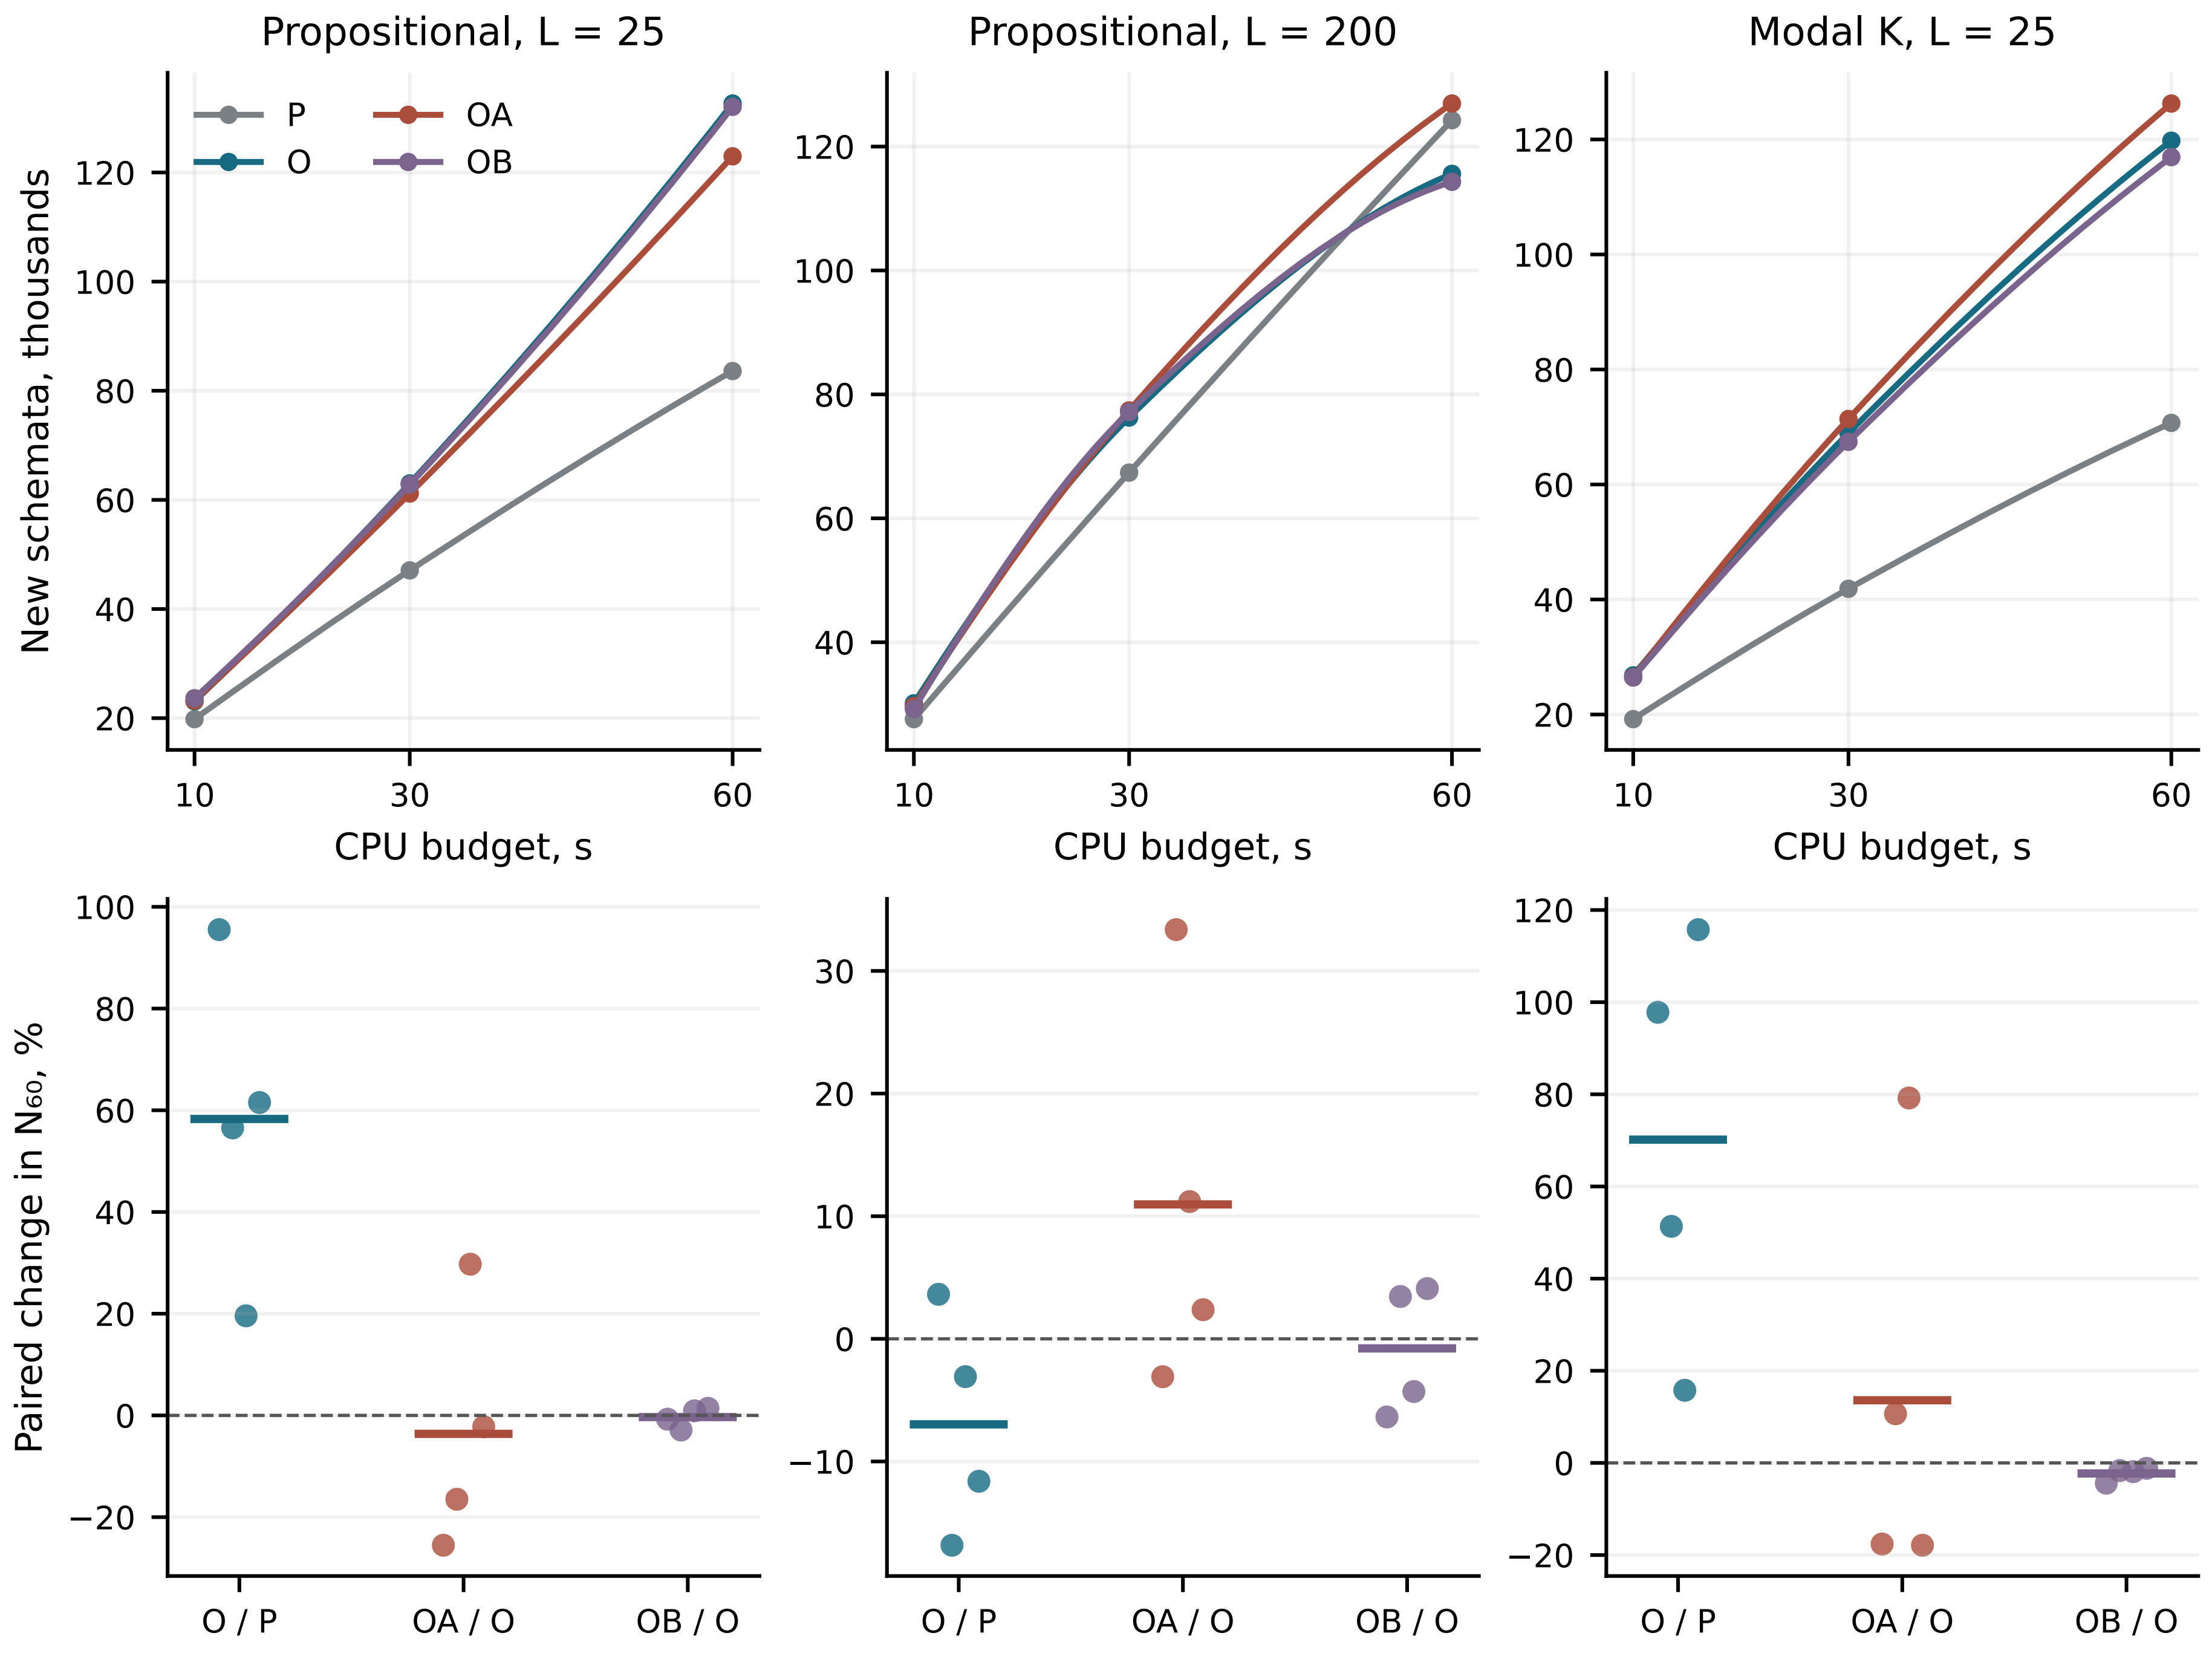
\includegraphics[width=\linewidth,height=.67\textheight,keepaspectratio]{Fig1.png}
\caption{Continuous growth across CPU budgets. The upper panels show means over four schedules; points show the readings at 10, 30, and 60 CPU-seconds, and monotone cubic splines guide the eye between them without adding observations. Each lower-panel point marks one paired relative difference at 60 seconds, and each short horizontal segment marks the mean of four such differences, not a confidence interval. These mean paired changes need not equal the changes from ratios of means in the text. The protocol defines P, O, OA, and OB}\label{fig:1}
\end{figure}

All 48 conditions stop without a software failure, but their stopping rules constrain the endpoint. The records contain 34 unfinished CPU frontiers, two total-time limits, one late commit, and 11 soft-memory stops. All memory stops occur at propositional \(L = 200\): four in O, three in OA, and four in OB; these outcomes remain in the table rather than implying 60 seconds of growth without a memory limit. Peak memory reaches 1.74 GiB because the program checks its soft 1.5 GiB threshold between layers, and the late-commit rule excludes 372 formulae.

The final active sets remain small even while their archives grow. O, OA, and OB contain 131--132 active formulae, including three or four original axioms, whereas P contains 1,444--2,160. The independent audit replays 11,404 checkpoints and 5,544,593 records across trajectories, including late records that the journal retains. This sum counts records rather than distinct theorems in the union and does not impose a bound on archive memory.

\subsection*{7.2 Proof reuse and human coverage}\label{proof-reuse-and-human-coverage}
\addcontentsline{toc}{subsection}{7.2 Proof reuse and human coverage}

The passive-library control reproduces all 3,503 paired search increments over common completed epochs, separating maintenance cost from changes in available premises. Earlier human diagnostics rank throughput and mathematical coverage differently: at size 25, bounded activity raises output whereas mean exact archive matches fall from 24 to 20.5. These controls motivate the new-frontier criterion. Appendices H and M report the lease, human-coverage, and branch comparisons.

\subsection*{7.3 Neutral continuation and empirical Pareto trade-offs}\label{neutral-continuation-and-empirical-pareto-trade-offs}
\addcontentsline{toc}{subsection}{7.3 Neutral continuation and empirical Pareto trade-offs}

The later frozen panel comprises 144 source trajectories, six pair-selection policies, three logic--size regimes, and eight scheduler states per regime. Each source supplies packages with up to 4, 16, or 64 anchors at nominal source ceilings of 60, 180, and 600 CPU-seconds. Separate neutral generators continue from those packages, giving 1,296 continuations with nested readings at 10, 30, and 60 CPU-seconds. The primary endpoint fixes the source ceiling at 180 CPU-seconds, the anchor cap at 16, and continuation at 30 CPU-seconds. Novelty excludes the union of concurrent source archives and the frozen training archives; Appendix I records the protocol and checks.

At this endpoint, the learned half-filter with deferred replay improves mean novelty over ungated growth in both propositional regimes, with eight positive pairs out of eight. The size-25 regime also improves the measured CPU and package-byte coordinates in every pair. The size-200 package grows by 16.5\% on average, illustrating why a useful skeleton need not minimise every resource coordinate. The modal comparison splits four wins and four losses despite a positive mean (Table 3).

\begingroup
\small
\setlength{\tabcolsep}{3pt}
\renewcommand{\arraystretch}{1.13}

\begin{longtable}[]{@{}
  >{\raggedright\arraybackslash}p{(\linewidth - 8\tabcolsep) * \real{0.1923}}
  >{\raggedleft\arraybackslash}p{(\linewidth - 8\tabcolsep) * \real{0.2053}}
  >{\raggedleft\arraybackslash}p{(\linewidth - 8\tabcolsep) * \real{0.1989}}
  >{\raggedleft\arraybackslash}p{(\linewidth - 8\tabcolsep) * \real{0.1307}}
  >{\raggedleft\arraybackslash}p{(\linewidth - 8\tabcolsep) * \real{0.2729}}@{}}
\caption{Neutral-continuation outcomes for ungated growth and learned half-selection with replay}\label{tab:3}\tabularnewline
\toprule\noalign{}
\begin{minipage}[b]{\linewidth}\raggedright
\textbf{Regime}
\end{minipage} & \begin{minipage}[b]{\linewidth}\raggedleft
\textbf{New schemata without gate}
\end{minipage} & \begin{minipage}[b]{\linewidth}\raggedleft
\textbf{Learned half with replay}
\end{minipage} & \begin{minipage}[b]{\linewidth}\raggedleft
\textbf{Positive pairs}
\end{minipage} & \begin{minipage}[b]{\linewidth}\raggedleft
\textbf{Chain CPU without gate / with replay}
\end{minipage} \\
\midrule\noalign{}
\endfirsthead
\toprule\noalign{}
\begin{minipage}[b]{\linewidth}\raggedright
\textbf{Regime}
\end{minipage} & \begin{minipage}[b]{\linewidth}\raggedleft
\textbf{New schemata without gate}
\end{minipage} & \begin{minipage}[b]{\linewidth}\raggedleft
\textbf{Learned half with replay}
\end{minipage} & \begin{minipage}[b]{\linewidth}\raggedleft
\textbf{Positive pairs}
\end{minipage} & \begin{minipage}[b]{\linewidth}\raggedleft
\textbf{Chain CPU without gate / with replay}
\end{minipage} \\
\midrule\noalign{}
\endhead
\bottomrule\noalign{}
\endlastfoot
Propositional, size 25 & 13,935.38 & 27,285.12 & 8/8 & 209.74 / 169.53 \\
Propositional, size 200 & 20,569.25 & 26,805.12 & 8/8 & 147.54 / 136.06 \\
Modal K, size 25 & 22,164.25 & 25,456.50 & 4/8 & 209.68 / 139.00 \\
\end{longtable}

\endgroup

The table reports means across eight scheduler states, not independent mathematical theories. Chain CPU includes credited work to build sources, select packages, and continue search, whereas training and later independent audit remain separate. Resource guards stop 119 sources at the memory threshold, 21 through the implementation's saturation condition, and four at the epoch cap; no source completes 600 CPU-seconds. The gains therefore characterise the observed resource-bounded trajectories rather than a completed long-horizon limit or a fixed-quality speedup.

The Pareto comparison fixes the primary source ceiling and continuation horizon while varying six policies and three anchor caps. Each regime contributes 18 mean triples. A setting enters the three-coordinate frontier when no other setting uses no more CPU or package bytes, yields at least as much novelty, and strictly improves at least one coordinate. The figure projects those triples onto CPU and novelty; outlined points mark the full three-coordinate frontier, so a point can remain nondominated through smaller package size even when its projection looks inferior (Fig. 2).

\begin{figure}[!htbp]
\centering
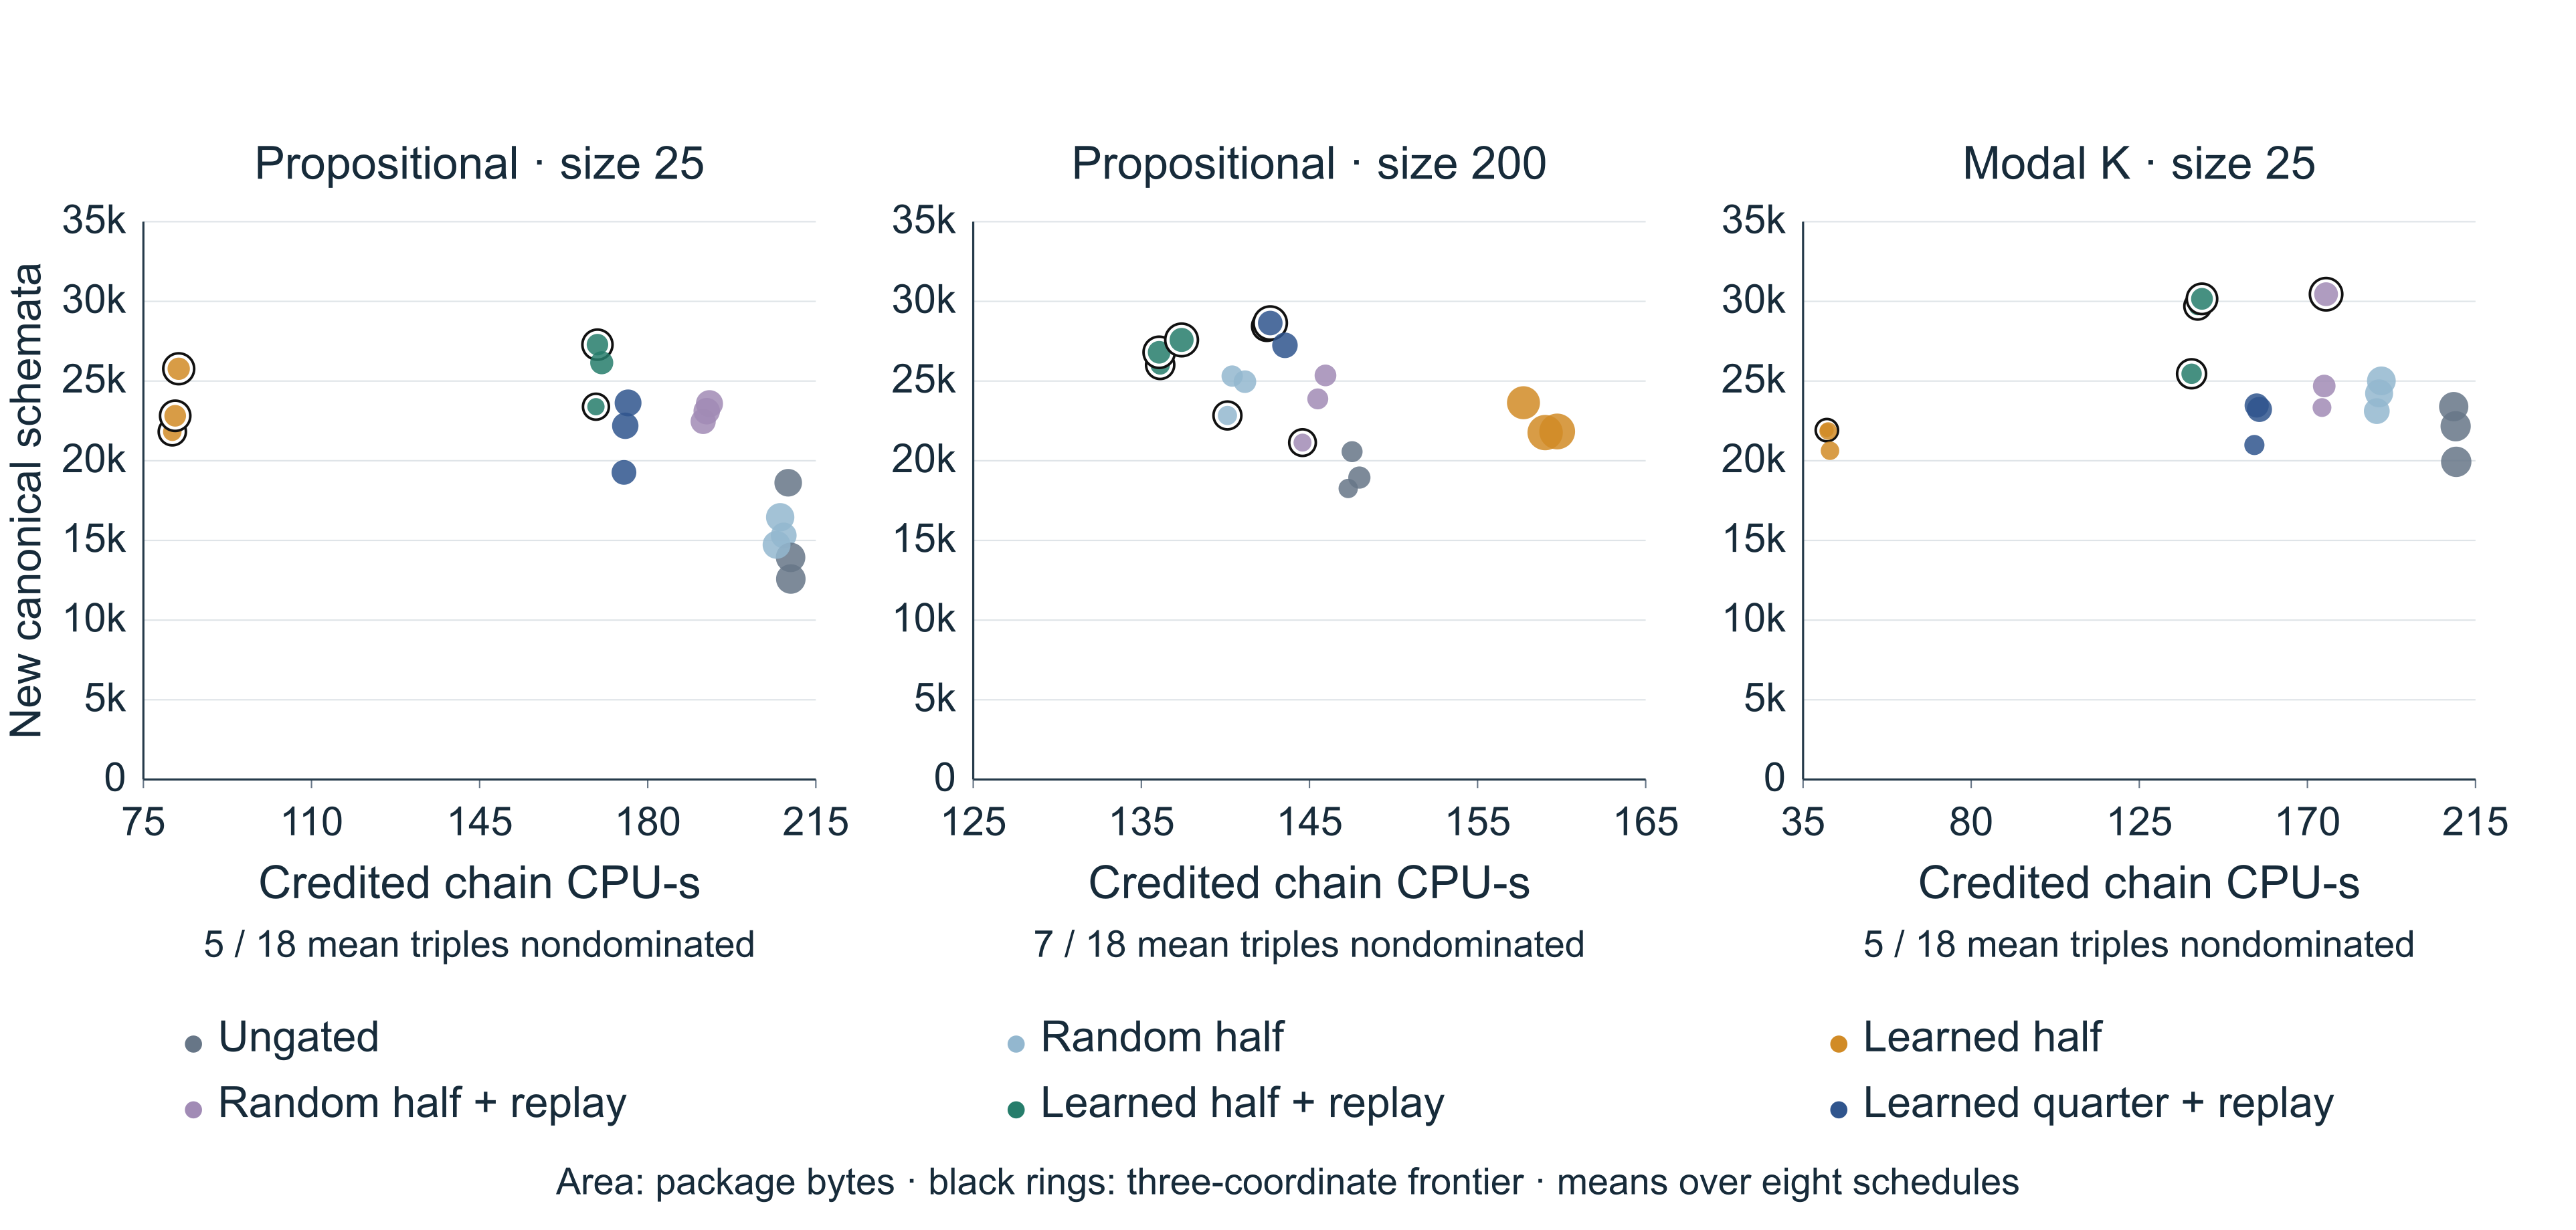
\includegraphics[width=\linewidth,height=.67\textheight,keepaspectratio]{Fig2.png}
\caption{Empirical Pareto trade-offs at a source ceiling of 180 CPU-seconds and continuation of 30 CPU-seconds. Colour identifies the pair policy, marker area indicates proof-backed package bytes, and outlines identify nondominated mean triples across CPU, bytes, and novelty. Each point averages eight scheduler states}\label{fig:2}
\end{figure}

These trade-offs favour different settings for different budgets. The learned half-filter without replay can cost less than replay at size 25, whereas replay yields more new schemata. More anchors or a later source slice need not improve continuation. The empirical frontier consequently supports a choice among useful finite skeletons, rather than a universal winner or an optimum beyond this grid.

\subsection*{7.4 Structural enrichment on the development reference}\label{structural-enrichment-on-the-development-reference}
\addcontentsline{toc}{subsection}{7.4 Structural enrichment on the development reference}

The short-programme compiler increases reference coverage while preserving the accumulated generator and previous library. The following means average six source states and both neutral continuers at eight growth CPU-seconds. Coverage excludes the 34 statements that initial axiom instances already cover. The common-frontier column instead excludes the union of all initial interfaces within the source block, so it measures genuinely additional reference capability under that comparison (Table 4).

\begingroup
\small
\setlength{\tabcolsep}{3pt}
\renewcommand{\arraystretch}{1.13}

\begin{longtable}[]{@{}
  >{\raggedright\arraybackslash}p{(\linewidth - 8\tabcolsep) * \real{0.3598}}
  >{\raggedleft\arraybackslash}p{(\linewidth - 8\tabcolsep) * \real{0.1601}}
  >{\raggedleft\arraybackslash}p{(\linewidth - 8\tabcolsep) * \real{0.1601}}
  >{\raggedleft\arraybackslash}p{(\linewidth - 8\tabcolsep) * \real{0.1601}}
  >{\raggedleft\arraybackslash}p{(\linewidth - 8\tabcolsep) * \real{0.1601}}@{}}
\caption{Initial and further reference coverage in the six-source development comparison}\label{tab:4}\tabularnewline
\toprule\noalign{}
\begin{minipage}[b]{\linewidth}\raggedright
\textbf{Library policy}
\end{minipage} & \begin{minipage}[b]{\linewidth}\raggedleft
\textbf{Initial coverage}
\end{minipage} & \begin{minipage}[b]{\linewidth}\raggedleft
\textbf{Final coverage}
\end{minipage} & \begin{minipage}[b]{\linewidth}\raggedleft
\textbf{Common frontier}
\end{minipage} & \begin{minipage}[b]{\linewidth}\raggedleft
\textbf{Derived anchors}
\end{minipage} \\
\midrule\noalign{}
\endfirsthead
\toprule\noalign{}
\begin{minipage}[b]{\linewidth}\raggedright
\textbf{Library policy}
\end{minipage} & \begin{minipage}[b]{\linewidth}\raggedleft
\textbf{Initial coverage}
\end{minipage} & \begin{minipage}[b]{\linewidth}\raggedleft
\textbf{Final coverage}
\end{minipage} & \begin{minipage}[b]{\linewidth}\raggedleft
\textbf{Common frontier}
\end{minipage} & \begin{minipage}[b]{\linewidth}\raggedleft
\textbf{Derived anchors}
\end{minipage} \\
\midrule\noalign{}
\endhead
\bottomrule\noalign{}
\endlastfoot
Early compressed source & 31.83 & 33.92 & 1.92 & 605.5 \\
Continued cumulative source plus codec & 31.00 & 33.58 & 1.58 & 929.2 \\
Persistent rule retrieval & 31.17 & 33.42 & 1.25 & 903.8 \\
Retrieval with coupled MP chains & 31.17 & 33.50 & 1.42 & 1043.3 \\
Structural synthesis & 35.83 & 37.75 & 1.92 & 628.5 \\
\end{longtable}

\endgroup

Structural synthesis exceeds the continued cumulative control in final coverage and coverage-curve area in all six source means. Its average synthesis stage takes 0.230 CPU-seconds; separate accounts charge coding, interface preparation, and checking. These incremental timings omit the initial source reload and historical acquisition costs, so they establish neither a complete speedup nor cheaper attainment of a fixed quality level. The early library matches its common-frontier score with fewer anchors, whereas coupled MP chains do not improve future quality (Fig. 3).

\begin{figure}[!htbp]
\centering
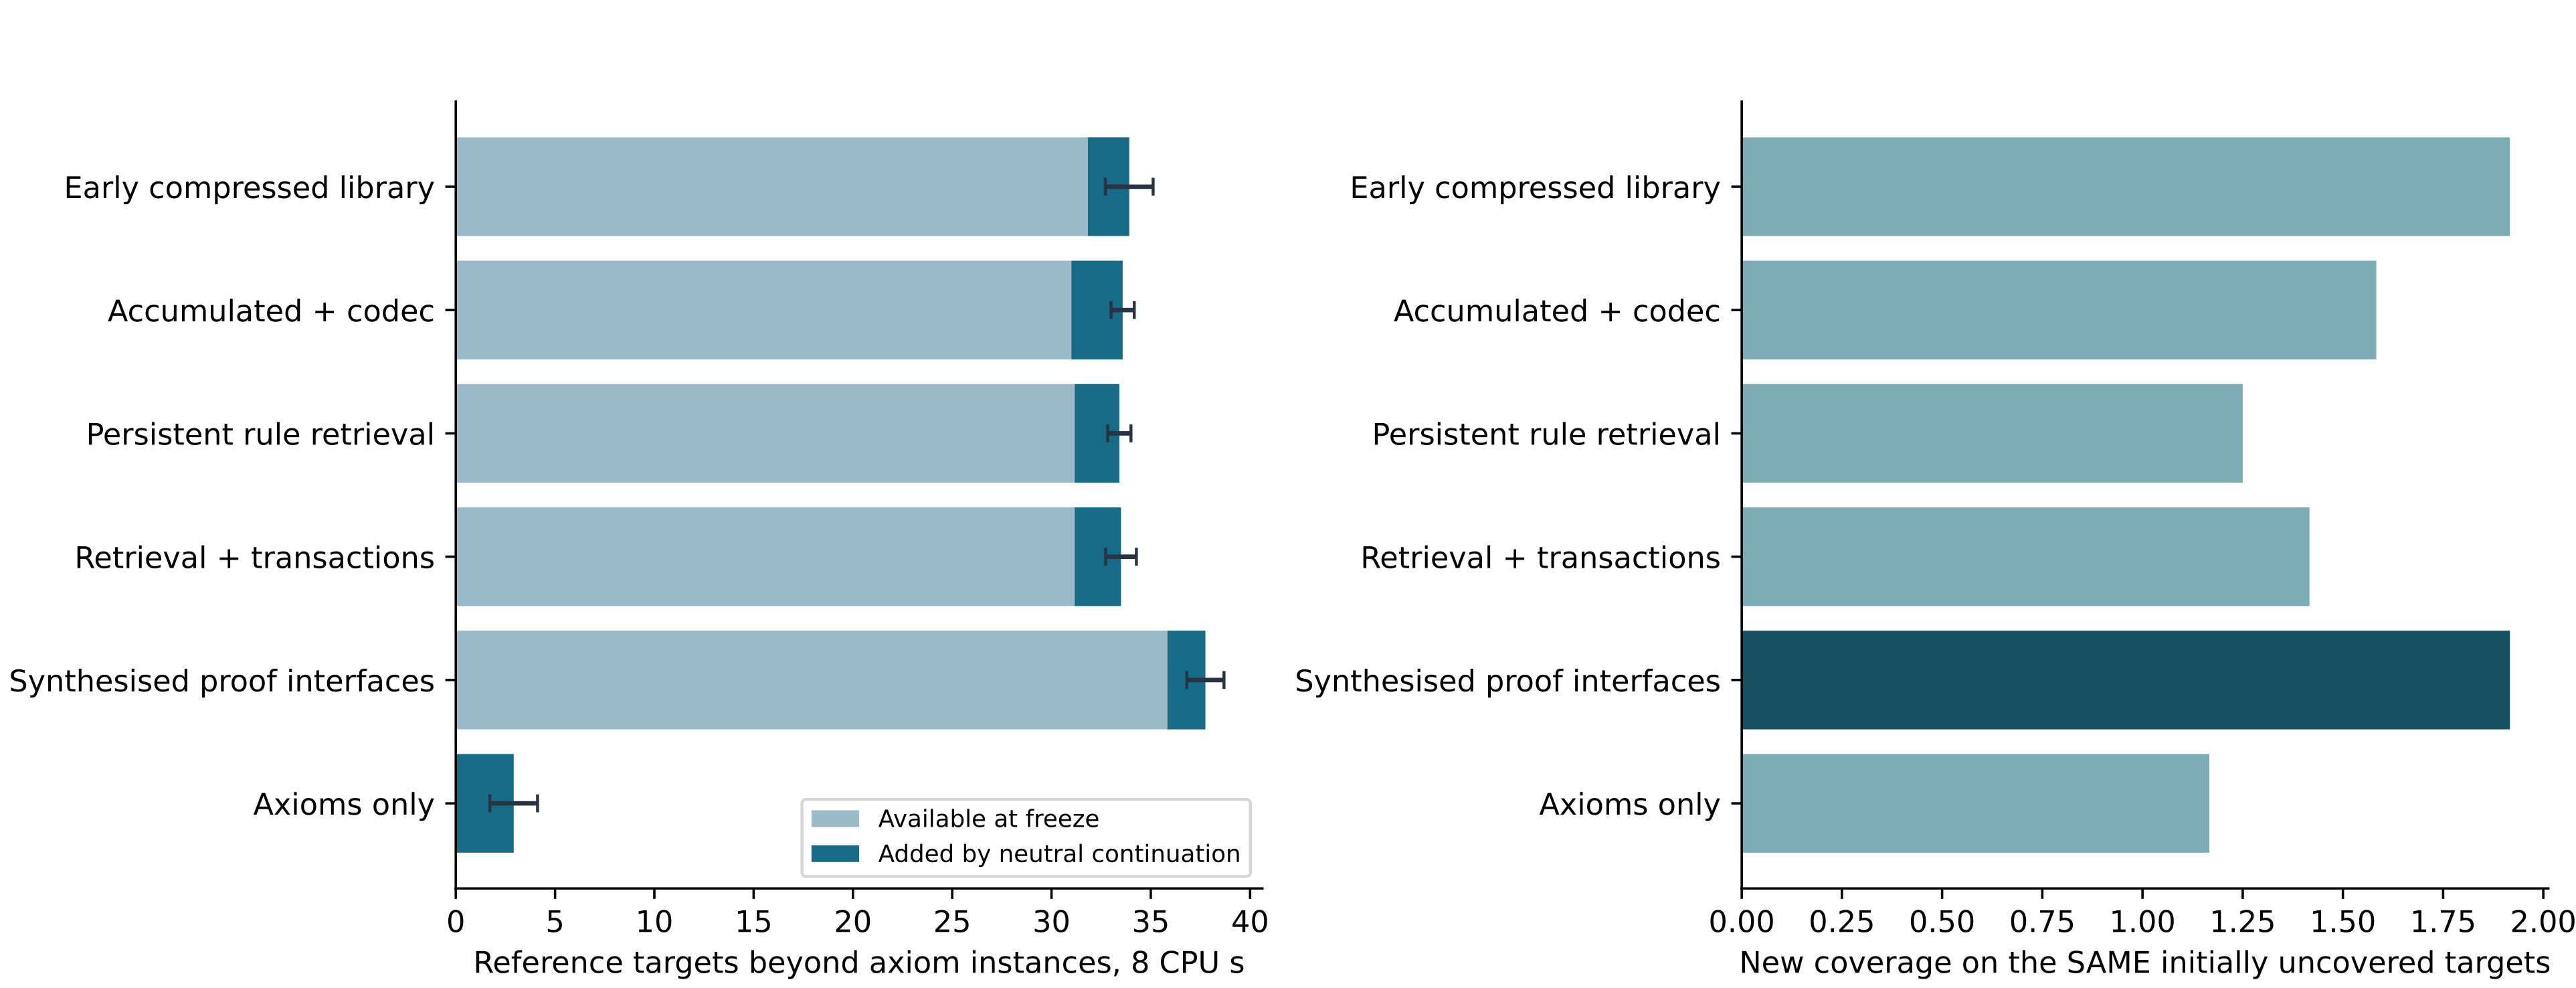
\includegraphics[width=\linewidth,height=.67\textheight,keepaspectratio]{Fig3.png}
\caption{Native development comparison at eight growth CPU-seconds. Left bars separate initial coverage from additional coverage, excluding axiom instances; whiskers show the standard deviation of the six source means, not confidence intervals. Right bars count new coverage on the same initially uncovered residual within each block. Two continuer views do not double the independent source count}\label{fig:3}
\end{figure}

The fixed short-grammar control identifies what produced the gain. At most two MP nodes yield four possible tree shapes including the boundary-only shape; every source already contains them. Replacing source-derived shapes with the whole fixed short grammar reproduces the same 21 requested formulae and identical certificates in all six cases. Source-specific shape learning therefore explains none of that experiment's output difference. Two of four additional initially covered statements follow from newly compiled schemata; the other two follow from archived schemata that the old interface omitted. These findings support checked structural enrichment, not adaptation or new mathematical theorems.

\subsection*{7.5 Locked native comparison}\label{locked-native-comparison}
\addcontentsline{toc}{subsection}{7.5 Locked native comparison}

All 16 source blocks and 160 planned continuations finish both registered horizons and pass independent replay. Each table entry averages the two neutral continuers within a source, then averages the 16 sources. Initial coverage counts all 963 reference targets; both future columns count only the common initially uncovered residual within that source block. Derived-anchor counts exclude 29 basis roots and separate certificate-only support (Table 5).

\begingroup
\small
\setlength{\tabcolsep}{3pt}
\renewcommand{\arraystretch}{1.13}

\begin{longtable}[]{@{}
  >{\raggedright\arraybackslash}p{(\linewidth - 8\tabcolsep) * \real{0.2558}}
  >{\raggedleft\arraybackslash}p{(\linewidth - 8\tabcolsep) * \real{0.1701}}
  >{\raggedleft\arraybackslash}p{(\linewidth - 8\tabcolsep) * \real{0.1865}}
  >{\raggedleft\arraybackslash}p{(\linewidth - 8\tabcolsep) * \real{0.2259}}
  >{\raggedleft\arraybackslash}p{(\linewidth - 8\tabcolsep) * \real{0.1617}}@{}}
\caption{Initial coverage, further common-residual coverage, and anchors in the locked native comparison}\label{tab:5}\tabularnewline
\toprule\noalign{}
\begin{minipage}[b]{\linewidth}\raggedright
\textbf{Library}
\end{minipage} & \begin{minipage}[b]{\linewidth}\raggedleft
\textbf{Initial coverage}
\end{minipage} & \begin{minipage}[b]{\linewidth}\raggedleft
\textbf{New at 60 growth s}
\end{minipage} & \begin{minipage}[b]{\linewidth}\raggedleft
\textbf{New at 90 operational s}
\end{minipage} & \begin{minipage}[b]{\linewidth}\raggedleft
\textbf{Derived anchors}
\end{minipage} \\
\midrule\noalign{}
\endfirsthead
\toprule\noalign{}
\begin{minipage}[b]{\linewidth}\raggedright
\textbf{Library}
\end{minipage} & \begin{minipage}[b]{\linewidth}\raggedleft
\textbf{Initial coverage}
\end{minipage} & \begin{minipage}[b]{\linewidth}\raggedleft
\textbf{New at 60 growth s}
\end{minipage} & \begin{minipage}[b]{\linewidth}\raggedleft
\textbf{New at 90 operational s}
\end{minipage} & \begin{minipage}[b]{\linewidth}\raggedleft
\textbf{Derived anchors}
\end{minipage} \\
\midrule\noalign{}
\endhead
\bottomrule\noalign{}
\endlastfoot
Common core and short rules & 25.00 & 1.312 & 1.344 & 633.6 \\
Fixed extended repertoire & 29.00 & 1.594 & 1.625 & 675.0 \\
Random extended repertoire & 26.38 & 1.500 & 1.562 & 680.4 \\
Adaptive test variant & 27.88 & 1.656 & 1.688 & 673.4 \\
Whole fixed catalogue & 44.00 & 1.562 & 1.594 & 1282.3 \\
\end{longtable}

\endgroup

The whole fixed catalogue initially covers 44 targets, versus 29 for the fixed extended repertoire, but reaches 1.56 versus 1.59 new common-residual targets at 60 growth CPU-seconds. This contrast illustrates why initial coverage cannot rank future capability. The adaptive score chooses three distinct rule sets and reaches 1.656 new residual targets, yet its paired advantage over the quota-matched fixed repertoire averages only 0.0625 targets at either endpoint (Table 6).

\begingroup
\small
\setlength{\tabcolsep}{3pt}
\renewcommand{\arraystretch}{1.13}

\begin{longtable}[]{@{}
  >{\raggedright\arraybackslash}p{(\linewidth - 6\tabcolsep) * \real{0.3000}}
  >{\raggedleft\arraybackslash}p{(\linewidth - 6\tabcolsep) * \real{0.2400}}
  >{\raggedleft\arraybackslash}p{(\linewidth - 6\tabcolsep) * \real{0.2400}}
  >{\raggedleft\arraybackslash}p{(\linewidth - 6\tabcolsep) * \real{0.2200}}@{}}
\caption{Paired adaptive-minus-control differences and Holm-adjusted tests at both registered horizons}\label{tab:6}\tabularnewline
\toprule\noalign{}
\begin{minipage}[b]{\linewidth}\raggedright
\textbf{Adaptive minus control}
\end{minipage} & \begin{minipage}[b]{\linewidth}\raggedleft
\textbf{Difference at 60 growth s}
\end{minipage} & \begin{minipage}[b]{\linewidth}\raggedleft
\textbf{Difference at 90 operational s}
\end{minipage} & \begin{minipage}[b]{\linewidth}\raggedleft
\textbf{Holm adjusted p}
\end{minipage} \\
\midrule\noalign{}
\endfirsthead
\toprule\noalign{}
\begin{minipage}[b]{\linewidth}\raggedright
\textbf{Adaptive minus control}
\end{minipage} & \begin{minipage}[b]{\linewidth}\raggedleft
\textbf{Difference at 60 growth s}
\end{minipage} & \begin{minipage}[b]{\linewidth}\raggedleft
\textbf{Difference at 90 operational s}
\end{minipage} & \begin{minipage}[b]{\linewidth}\raggedleft
\textbf{Holm adjusted p}
\end{minipage} \\
\midrule\noalign{}
\endhead
\bottomrule\noalign{}
\endlastfoot
fixed & +0.06250 & +0.06250 & 1.000 \\
random & +0.15625 & +0.12500 & 1.000 \\
fixed all & +0.09375 & +0.09375 & 1.000 \\
\end{longtable}

\endgroup

Every Holm-adjusted p-value equals 1.000, and no contrast reaches the registered mean margin of one additional target at both clocks. We therefore retain fixed structural rules in the working architecture and do not attribute a confirmed gain to adaptive catalogue ranking. Appendix L reports the full paired comparison, statistical rule, and technical amendment.

The independent audit reconstructs 4,174,478 admission events and 2,846 hidden-support rediscovery witnesses, checks all target positions, and reproduces the endpoints and decision. These counts include repeated events across trajectories, not independent theorems. The comparison charges the full recorded catalogue to every arm under the shared backend; it does not test a specialised static implementation that avoids compiling unused entries.

\subsection*{7.6 Metamath and generated proof networks}\label{metamath-and-generated-proof-networks}
\addcontentsline{toc}{subsection}{7.6 Metamath and generated proof networks}

The network comparison follows the cumulative method through its delivered library and certificate support. Panel b uses the first source, 2026102201, with the quota-matched fixed structural repertoire. Appendix N presents the profiles of both variants and the separately preselected adaptive image. Both representatives follow the first-source convention, independently of target coverage, graph appearance, and power-law p-values.

All objects share the explicit native basis from the pinned \path{set.mm} revision \citep{MetamathSetMMPinned}: 25 logical or set-theoretic axioms and rules, six definitions, and 12 syntax assertions. Twenty-nine closed source schemata initialise search. The inherited proof-closed core contains 2,708 statements; the cumulative constructor continues that core, filters and revisits opportunities, applies reversible rot-pruning, compiles structural rules, and codes recurrent proofs. Panel b shows the delivered interface and every ancestor that its certificates require, not the full inherited archive. Appendix J preserves the earlier native study, whereas Appendix N records the new sources, projections, and metrics.

The first-source fixed library provides 675 derived anchors and 29 basis roots; 137 further vertices supply certificate-only support. Its projection therefore contains 841 vertices and 1,573 directed arcs. Across all 16 fixed sources, anchor counts range from 665 to 682, with a mean of 675.0; projected sizes range from 836 to 852. Hidden support does not confer search rights, and a verifier can expand every anchor to the original basis.

An arc runs from a premise to the conclusion that cites it. We omit primitive rule vertices and collapse repeated arcs in every object. Certificates retain joint premise roles, substitutions, and side conditions that this ordinary graph projection cannot express. The human fragment contains 2,306 named assertions whose actual proofs use only the declared basis, including assertions with essential hypotheses. Native vertices denote closed schemata with mandatory distinct-variable conditions. A shared basis does not eliminate the difference between named human steps and elementary native inferences.

The full reference enumerates all admitted MP steps through most-general unification and prescribed generalisations through proof height three, without skeleton-selection or formula-size cuts. Its 11,772 statements support both first-proof and all-inference projections. This reference supplies a complete finite slice of the stated operator, not all substitution instances, a deductive fixed point, or infinite closure of Zermelo--Fraenkel set theory with choice (ZFC). Panel b reaches certificate height 23; the comparison holds neither depth nor construction cost constant (Fig. 4).

\begin{figure}[!htbp]
\centering
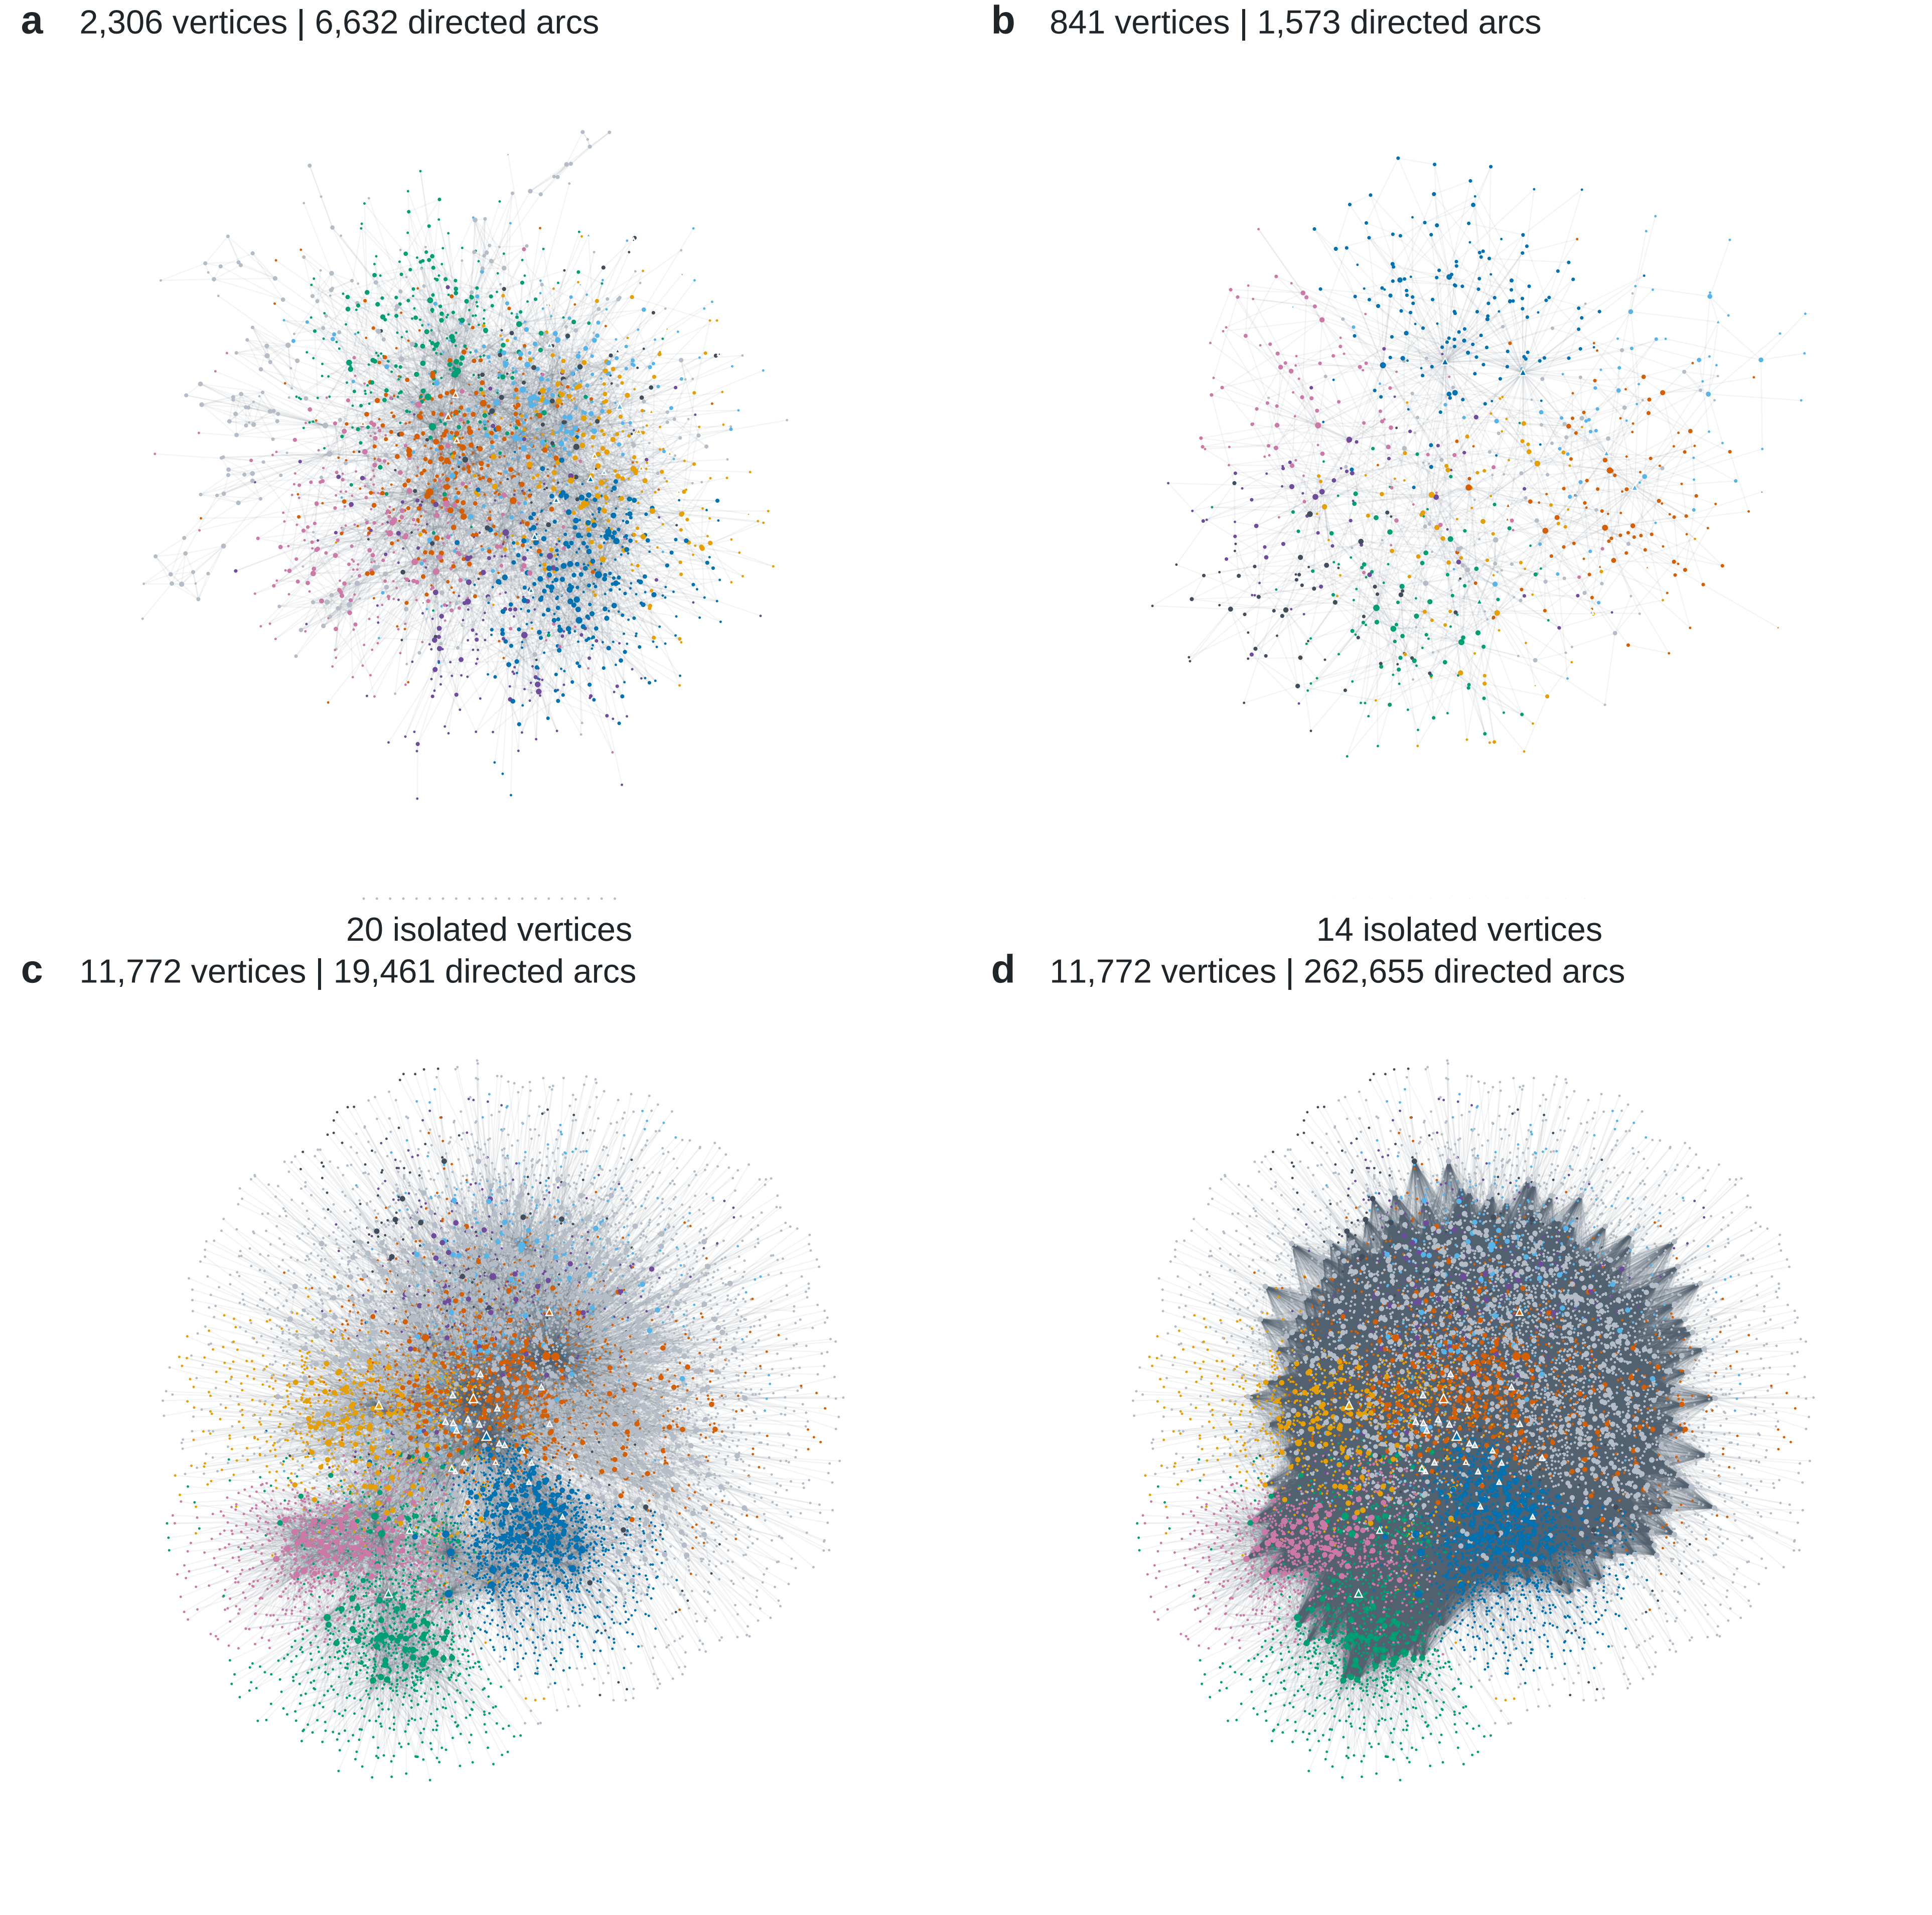
\includegraphics[width=\linewidth,height=.67\textheight,keepaspectratio]{Fig4.png}
\caption{Native proof networks on one explicit basis. a shows the compatible named Metamath fragment; b shows the first-source cumulative skeleton with fixed structural rules, including all certificate support; c shows first proofs in the complete height-three operator slice; d shows all enumerated inferences on those same vertices. Every vertex and unique undirected edge enters the drawing; only arrowheads disappear. Colours distinguish the eight largest communities in a, b, and c, with smaller communities in grey. d inherits c's coordinates, colours, and vertex areas; its tabulated modularity follows its own community search. Triangles mark the 29 basis roots. Areas increase with log reuse. Separate layouts do not measure comparable semantic distances}\label{fig:4}
\end{figure}

The representative skeleton reaches modularity 0.622, versus 0.539 across ten degree-preserving controls, and outgoing distinct-use degree yields a Gini coefficient of 0.731. Across the 16 fixed sources, modularity ranges from 0.622 to 0.629, with a mean of 0.625. These measurements characterise concentrated reuse and modular structure without promoting a single image to a mean result.

The new outgoing-degree profiles also differ from the earlier 2,708-vertex core. None of the 16 fixed-repertoire sources rejects the pure discrete power-law family at five percent; bootstrap p-values range from 0.24190 to 0.62575. The representative fits an exponent of 2.044719 from degree one, with 524 tail observations and p = 0.54640. Its other 317 vertices carry zero outgoing degree. On this same tail, the cutoff power law and rounded lognormal yield descriptive log likelihoods of \ensuremath{-}815.753 and \ensuremath{-}816.024, versus \ensuremath{-}818.182 for the pure power law. Compatibility with the pure family therefore does not select it uniquely or establish an infinite scale-free growth mechanism (Table 7).

\begingroup
\small
\setlength{\tabcolsep}{3pt}
\renewcommand{\arraystretch}{1.13}

\begin{longtable}[]{@{}
  >{\raggedright\arraybackslash}p{(\linewidth - 8\tabcolsep) * \real{0.3199}}
  >{\raggedleft\arraybackslash}p{(\linewidth - 8\tabcolsep) * \real{0.1700}}
  >{\raggedleft\arraybackslash}p{(\linewidth - 8\tabcolsep) * \real{0.1700}}
  >{\raggedleft\arraybackslash}p{(\linewidth - 8\tabcolsep) * \real{0.1700}}
  >{\raggedleft\arraybackslash}p{(\linewidth - 8\tabcolsep) * \real{0.1700}}@{}}
\caption{Network metrics for Metamath, the cumulative skeleton, and two complete height-three projections}\label{tab:7}\tabularnewline
\toprule\noalign{}
\begin{minipage}[b]{\linewidth}\raggedright
\textbf{Metric}
\end{minipage} & \begin{minipage}[b]{\linewidth}\raggedleft
\textbf{a Metamath}
\end{minipage} & \begin{minipage}[b]{\linewidth}\raggedleft
\textbf{b Cumulative skeleton}
\end{minipage} & \begin{minipage}[b]{\linewidth}\raggedleft
\textbf{c First proofs}
\end{minipage} & \begin{minipage}[b]{\linewidth}\raggedleft
\textbf{d All inferences}
\end{minipage} \\
\midrule\noalign{}
\endfirsthead
\toprule\noalign{}
\begin{minipage}[b]{\linewidth}\raggedright
\textbf{Metric}
\end{minipage} & \begin{minipage}[b]{\linewidth}\raggedleft
\textbf{a Metamath}
\end{minipage} & \begin{minipage}[b]{\linewidth}\raggedleft
\textbf{b Cumulative skeleton}
\end{minipage} & \begin{minipage}[b]{\linewidth}\raggedleft
\textbf{c First proofs}
\end{minipage} & \begin{minipage}[b]{\linewidth}\raggedleft
\textbf{d All inferences}
\end{minipage} \\
\midrule\noalign{}
\endhead
\bottomrule\noalign{}
\endlastfoot
Vertices \(N\) & 2306 & 841 & 11772 & 11772 \\
Directed arcs \(E\) & 6632 & 1573 & 19461 & 262655 \\
Largest-component vertices & 2286 & 827 & 11772 & 11772 \\
Isolated vertices & 20 & 14 & 0 & 0 \\
Mean local clustering \(C\) & 0.0689 & 0.0202 & 0.0347 & 0.3382 \\
Mean shortest path \(L\) & 4.137 & 4.177 & 4.334 & 3.213 \\
Diameter \(D\) & 11 & 8 & 6 & 4 \\
Modularity \(Q\) & 0.568 & 0.622 & 0.675 & 0.058 \\
Reference modularity \(Q_{0}\) & 0.401 & 0.539 & 0.599 & 0.053 \\
Small-world ratio \(\sigma_{DP}\) & 3.990 & 0.636 & 0.592 & 0.417 \\
Tail observations & 205 & 524 & 63 & 41 \\
Pure power law p & 0.09895 & 0.54640 & 0.01080 & 0.36490 \\
\end{longtable}

\endgroup

Table columns follow the figure panels. C, L, D, and Q refer to simple undirected projections. C assigns zero below degree two; L and D refer to the largest connected component and use every observed breadth-first-search (BFS) source. Panel a contains 20 isolates and panel b contains 14 unused basis roots; panels c and d remain connected. Q0 averages ten simple degree-preserving controls, with three Louvain starts for every observed and control graph. Panel b's control paths also use every source; the retained c and d controls estimate paths from 64 sources. The tail test for outgoing distinct-use degree fixes 20,000 bootstrap draws and refits both threshold and exponent. Appendix N reports all 32 new profiles and their scope.

The c--d pair isolates an edge-recording effect on identical statements: alternative edges raise clustering from 0.0347 to 0.3382, shorten the mean path from 4.334 to 3.213, and lower modularity from 0.675 to 0.058. No logical or vertex change explains that contrast. The ordinary proof-network profile therefore depends materially on how the representation records alternative derivations.

Newman \citep{Newman2003}, in \emph{The Structure and Function of Complex Networks}, treats degree heterogeneity, clustering, paths, and correlations as complementary features. Humphries and Gurney \citep{HumphriesGurney2008}, in \emph{Network `Small-World-Ness': A Quantitative Method for Determining Canonical Network Equivalence}, formalise the clustering--path comparison behind the small-world ratio. Under the declared degree-preserving reference, Metamath reaches a ratio of 3.990, whereas the skeleton reaches 0.636. Thus, the skeleton exhibits concentrated reuse, modular organisation, and a compatible conditional power-law tail, but its short paths do not establish small-world structure. These objects display distinct complex-network profiles rather than a division between networks and `mere graphs'. A conditional tail fit does not establish infinite scale invariance, and network metrics complement rather than replace future-use tests \citep{ClausetEtAl2009,BroidoClauset2019}. Ten null graphs support descriptive contrasts rather than a rank-test claim below five percent.

\section*{8 Discussion and scope}\label{discussion-and-scope}
\addcontentsline{toc}{section}{8 Discussion and scope}

The experiments establish that proof validity, compact proof code, and productive premise use answer different questions. The architecture preserves every accepted certificate while the policy changes which proven formulae can take part in new inferences. Internal controls measure the computational consequences of that change. Fragment reuse alone does not determine the return from an active slot, as the utility problem for acquired knowledge predicts \citep{Minton1990Utility}.

Bounded activity improves formula output in both size-25 configurations while keeping the active set roughly an order of magnitude smaller. Its lower count of matches to the chosen human statements identifies a second design objective: preserving useful mathematical anchors alongside high-throughput growth. The prospective panel shows that these objectives need not rank policies identically.

The O--P contrast tests a package of choices rather than isolated mechanisms. It does not identify separate causal effects of leases, quotas, frontier preservation, or returns to the active set. Appendix M reports the component comparisons that informed the cumulative architecture.

The scheduler repeats and resource guards restrict general claims. Four states vary the schedule within a formal configuration rather than sample independent theories, and the 10-, 30-, and 60-second readings share nested prefixes. Eleven size-200 trajectories reach the soft memory threshold, so their outcomes do not reveal what unlimited memory would permit. Every condition uses an append-only journal, so the O--P contrast does not measure a switch to incremental storage. Bounded active sets still allow archives, indices, and total memory to grow.

The coding library stores exact closed first proofs rather than shortest proofs. The structural extension separately derives general closed schemata by discharging open MP boundaries. The archive already shares identical subproofs in a directed acyclic graph (DAG), so shorter expanded terms do not demonstrate further compression of that graph. Repeated fragment use and conservative lemma synthesis preserve formal meaning; the costed future-growth test measures their operational value.

Human references expose differences that raw formula counts conceal. The historical 108-statement and native 919-statement references already informed development; they do not supply independent confirmation. The locked comparison evaluates a previously unscored 963-target POI subset only after every search trajectory freezes; a separate independent audit then checks the outcome. None of these corpora supplies a complete modal reference or an assessment of the whole mathematical value of the generated library.

The native network study adds a structural result to the operational evidence. A proof-closed skeleton exhibits modular organisation and concentrated reuse, whereas the fixed-vertex reference shows that alternative proof edges can strongly alter the same network metrics. Verified certificates, human-statement coverage, and measured continuation complement this structural profile. The native network study and the earlier pair-selection trajectories retain their separate scopes.

The combinatorial claims also require distinct scopes. The exponential lower bound counts explicit theorem instances, whereas the result for canonical schemata establishes only unboundedness. Neither the theorems nor finite runs establish non-computability of a bounded slice, exponential growth of schemata, or the limiting topology of an infinite proof space. Since the two logics change their language, axioms, and rules together, they do not isolate logic alone as a cause.

The native comparison supplies a reproducible operating configuration with fixed structural rules. Goal-directed proof search and control towards prescribed graph properties define the next two research tracks. For knowledge-based AI, our method preserves certified knowledge, changes which statements inference may use, and accounts for the required resources.

\section*{9 Conclusions}\label{conclusions}
\addcontentsline{toc}{section}{9 Conclusions}

We formulate the direct, inverse, and control cognition problems for formal knowledge. The direct cognition problem generates a proof skeleton without a final target theorem. The inverse problem takes a particular statement and seeks intermediate lemmas that connect it to the existing base (current skeleton), to certify its status relative to the chosen formal system. This requires a proof of the statement, a proof of its negation, or a separate independence argument; unsuccessful search returns unknown. The control problem selects a growth regime to obtain a graph with desirable properties such as modularity, concentrated reuse, or a particular degree distribution.

We develop a cumulative method that generates a semantic skeleton through checkable anchor statements and expandable proofs. The method addresses the direct cognition problem by separating archived proofs, active premises, and reusable lemma entries. Premise filtering, deferred replay, and reversible deactivation regulate immediate work; positive-marginal coding retains recurrent proof fragments; a structural compiler derives general lemma schemata with elementary certificates. The theoretical results establish conservative proof recovery and the output obstruction to complete explicit storage under fixed capacity.

The experiments assess future capability rather than count retained formulae alone. In the 144-source continuation panel, learned pair selection with deferred replay raises mean novelty over ungated growth by 95.8\% and 30.3\% in the two propositional regimes, with eight positive pairs in each and lower mean credited chain CPU. Modal outcomes and resource guards delimit the claim. Empirical Pareto sets retain the finite trade-offs among CPU, package bytes, and future output rather than name a universal winner.

The native architecture carries the accumulated method onto an explicit Metamath basis with checked structural rules and controlled access to certificate support. The locked 963-target test completes 160 continuations across 16 source blocks and passes independent replay. The registered comparison does not confirm an adaptive advantage; fixed structural rules supply the final repertoire. The locked comparison separates initial coverage from newly reached reference statements.

The new network comparison characterises the resulting certified skeleton alongside human mathematics and finite exhaustive growth. The first-source fixed skeleton contains 841 certificate vertices and reaches modularity 0.622; all 16 profiles quantify variation. Their outgoing-degree diagnostics do not reject a pure power-law tail, although alternative models also fit and the finite experiment establishes no limiting law. On the identical 11,772 vertices of the complete height-three slice, alternative proof edges raise clustering from 0.0347 to 0.3382 while lowering modularity from 0.675 to 0.058. These measurements connect useful finite proof libraries to network structure.

The principal result answers the direct question through an executable proof-preserving method, a future-use criterion, and an explicit cost account. It supports continued inference from finite certified skeletons in the tested regimes and connects their operational use to measurable network structure. This checked backbone supplies the first stage of the proposed programme: generate reusable skeleton anchors, then extend their neighbourhoods when a task requires further knowledge. Target-directed reasoning, optional generative tools for local extensions, and deliberate graph objectives define the inverse and control tracks; the current experiments test the backbone rather than those future components.

\section*{10 Reproducibility}\label{reproducibility}
\addcontentsline{toc}{section}{10 Reproducibility}

The reproducibility records link every new numerical claim to its protocol, code, and source results. All 16 blind receipts, the one-shot evaluation, the completed pipeline, and the independent review refer to the corrected seal in Appendix L. The auditor rechecks permitted inference, target-instance certificates, common residuals, and the statistical decision. Appendices A--N retain proofs, historical controls, benchmark provenance, and network records. The editorial manifest checks input hashes and identifies the first-source images.

\textbf{Computing resources.} The prospective panels ran locally under process-CPU budgets. The cluster experiments used one CPU per condition; Appendix F records the execution environment.

\section*{Appendix A. Combinatorial bounds and resources}\label{appendix-a.-combinatorial-bounds-and-resources}
\addcontentsline{toc}{section}{Appendix A. Combinatorial bounds and resources}

\subsection*{A.1. Resources and notation}\label{a.1.-resources-and-notation}
\addcontentsline{toc}{subsection}{A.1. Resources and notation}

Resource accounting distinguishes the active representation \(M_{S}\), reserve \(M_{P}\), archive \(M_{\Omega}\), and peak process memory. Moving a proof to disk does not discard knowledge. Equal numbers of anchors therefore imply neither equal certificate sizes nor equal memory use (Table 8).

\begingroup
\small
\setlength{\tabcolsep}{3pt}
\renewcommand{\arraystretch}{1.13}

\begin{longtable}[]{@{}
  >{\raggedright\arraybackslash}p{(\linewidth - 2\tabcolsep) * \real{0.1707}}
  >{\raggedright\arraybackslash}p{(\linewidth - 2\tabcolsep) * \real{0.8293}}@{}}
\caption{Notation, mathematical objects, and resource units}\label{tab:8}\tabularnewline
\toprule\noalign{}
\begin{minipage}[b]{\linewidth}\raggedright
\textbf{Notation}
\end{minipage} & \begin{minipage}[b]{\linewidth}\raggedright
\textbf{Object and unit}
\end{minipage} \\
\midrule\noalign{}
\endfirsthead
\toprule\noalign{}
\begin{minipage}[b]{\linewidth}\raggedright
\textbf{Notation}
\end{minipage} & \begin{minipage}[b]{\linewidth}\raggedright
\textbf{Object and unit}
\end{minipage} \\
\midrule\noalign{}
\endhead
\bottomrule\noalign{}
\endlastfoot
\(|F|_{AST}\) & Number of all syntax-tree vertices; metric for the main bounds \(L = 25,200\) \\
\(\ell_{leaf}(F)\) & Number of leaves; metric for the separate implicational KSP benchmark \\
\(H_{d}^{sch}\) & Canonical schemata through depth \(d\) under the declared constraints \\
\(H_{4}\) & Small exact schematic benchmark through depth 4, with every stored schema of size at most 25 \\
H14 & Name of an earlier configuration, not depth 14 or benchmark \(H_{4}\) \\
\(\Omega_{0},\Omega_{b}\) & Common initial archive and archive of a verified continuation \\
\end{longtable}

\endgroup

The relation between the two size metrics depends on the language. A purely implicational formula satisfies \(|F|_{AST} = 2\ell_{leaf}(F) - 1\), whereas negation or modality invalidates this equality. Budget \(b\) covers the declared computational scope; accounting records the historical cost of constructing \(\Omega_{0}\) separately.

\subsection*{A.2. Combinatorial costs and finite approximation}\label{a.2.-combinatorial-costs-and-finite-approximation}
\addcontentsline{toc}{subsection}{A.2. Combinatorial costs and finite approximation}

\subsubsection*{A.2.1. Number of potential pairs}\label{a.2.1.-number-of-potential-pairs}
\addcontentsline{toc}{subsubsection}{A.2.1. Number of potential pairs}

Two-premise modus ponens admits an exact count of potential pairs before filtering. Let \(V_{\leq d}\) contain the available formulae, \(F_{d}\) denote the new frontier, \(I_{\leq d}\) denote the implicational major premises, and \(F_{d}^{I} = F_{d} \cap I_{\leq d}\). Restricting attention to pairs with at least one new premise gives

\[\fitdisplay{P_{d} = |F_{d}|\,|I_{\leq d}| + |V_{< d}|\,|F_{d}^{I}|.}\]

The two terms divide the ordered pairs by premise role. The first term counts a new minor premise, including pairs with two new premises; the second counts a new major premise and an old minor premise. This equality describes Cartesian enumeration under that division of roles; structural indexing reduces actual checks, whereas other rules require their own counters.

The potential-pair count satisfies \(P_{d} \leq N_{d}^{2}\) for \(N_{d} = |V_{\leq d}|\). A single check also incurs costs for formula size, unification, and side conditions. The inequality thus bounds pairs, not the generator's total running time, and schemata with several matching results can produce more conclusions than their pair count alone suggests.

\subsubsection*{A.2.2. Exponential size of the explicit representation}\label{a.2.2.-exponential-size-of-the-explicit-representation}
\addcontentsline{toc}{subsubsection}{A.2.2. Exponential size of the explicit representation}

An explicit-space lower bound requires a precise vertex convention. In the following result, each vertex represents a syntactically distinct formula, not a logical-equivalence class or all instances of one schema. We use a language with one fixed propositional letter \(p\), implication, and negation, and count abstract-syntax-tree vertices in \(|F|\); the calculus contains modus ponens and the schemata

\[\fitdisplay{\begin{matrix}
K(A,B) = A \rightarrow (B \rightarrow A), \\
S(A,B,C) = \lbrack A \rightarrow (B \rightarrow C)\rbrack \rightarrow \lbrack(A \rightarrow B) \rightarrow (A \rightarrow C)\rbrack
\end{matrix}}\]

The lower bound needs no additional axioms, including neither the third classical schema nor modal axioms. Let \(T_{L}\) denote the formulae admitting a proof in which \textbf{every} formula, including each axiom instance, contains at most \(L\) syntax-tree vertices. This definition expands axiom-schema substitutions explicitly and keeps the letter \(p\) fixed in the resulting formulae.

\textbf{Theorem 1 (full statement): size of the explicit proof space.} For every integer \(m \geq 0\),

\[\fitdisplay{|T_{18m + 17}|\  \geq \ {Cat}_{m},\quad\quad{Cat}_{m} = \frac{1}{m + 1}\binom{2m}{m}.}\]

These \({Cat}_{m}\) conclusions all contain \(4m + 3\) syntax-tree vertices. Each admits a proof with at most two modus-ponens applications along any path, counting axiom instances at height zero. As \(m \rightarrow \infty\), their number satisfies

\[\fitdisplay{{Cat}_{m} \sim \frac{4^{m}}{\sqrt{\pi}\, m^{3/2}}.}\]

\textbf{Proof.} Count fully parenthesised implicational formulae with \(m\) occurrences of \(\rightarrow\) and \(m + 1\) leaves that each carry the label \(p\). Let \(\mathcal{B}_{m}\) contain all such formulae. Splitting at the left and right subtrees gives

\[\fitdisplay{|\mathcal{B}_{0}| = 1,\quad\quad|\mathcal{B}_{m}| = \sum_{j = 0}^{m - 1}|\mathcal{B}_{j}|\,|\mathcal{B}_{m - 1 - j}|.}\]

This recurrence gives the standard Catalan enumeration of ordered full binary trees \citep{FlajoletSedgewick2009}. For each \(F \in \mathcal{B}_{m}\), set \(I_{F} = F \rightarrow F\); the map \(F \mapsto I_{F}\) injects the family into distinct conclusions, and the common leaf label prevents variable renaming from merging different tree shapes. With \(s = |F| = 2m + 1\), the size of each conclusion equals \(|I_{F}| = 2s + 1 = 4m + 3\).

The following derivation proves \(I_{F}\) and exposes every intermediate formula. Its two modus-ponens steps use only instances of \(K\) and \(S\). We can therefore check the size bound directly:

\[\fitdisplay{\begin{matrix}
\alpha = F \rightarrow \lbrack(F \rightarrow F) \rightarrow F\rbrack,\quad\quad K(F,F \rightarrow F), \\
\beta = \alpha \rightarrow \{\lbrack F \rightarrow (F \rightarrow F)\rbrack \rightarrow (F \rightarrow F)\},\quad\quad S(F,F \rightarrow F,F), \\
\gamma = \lbrack F \rightarrow (F \rightarrow F)\rbrack \rightarrow (F \rightarrow F),\quad\quad MP(\alpha,\beta), \\
\delta = F \rightarrow (F \rightarrow F),\quad\quad K(F,F), \\
I_{F} = F \rightarrow F,\quad\quad MP(\delta,\gamma).
\end{matrix}}\]

The respective sizes of the five formulae equal \(4s + 3\), \(9s + 8\), \(5s + 4\), \(3s + 2\), and \(2s + 1\). Their maximum equals \(9s + 8 = 18m + 17\), so every \(I_{F}\) belongs to \(T_{18m + 17}\). Applying Stirling's formula to \({Cat}_{m}\) gives the asymptotic estimate. \(\square\)

The theorem bounds output size, without claiming a new complexity result for finding an individual proof. The standard identity derivation and Catalan count provide an explicit witness; the displayed derivation supplies the constant \(18\), without any claim of optimality. For \(L \geq 17\), setting \(m = \lfloor(L - 17)/18\rfloor\) yields

\[\fitdisplay{|T_{L}| \geq {Cat}_{\lfloor(L - 17)/18\rfloor} = \Omega\left( \frac{2^{L/9}}{L^{3/2}} \right)\quad(L \rightarrow \infty).}\]

\subsubsection*{A.2.3. Limits of complete storage under a fixed resource bound}\label{a.2.3.-limits-of-complete-storage-under-a-fixed-resource-bound}
\addcontentsline{toc}{subsubsection}{A.2.3. Limits of complete storage under a fixed resource bound}

\textbf{Corollary 1.} An algorithm that materialises and retains a separate record for every formula in \(T_{L}\) requires \(\Omega({Cat}_{m})\) records and output operations when \(L = 18m + 17\). If each record contains a separate syntax tree without sharing, the family's conclusions alone require \(\Omega(m{Cat}_{m})\) symbols. Sharing subexpressions can reduce the second bound, but cannot reduce the number of explicitly addressable vertices under this model.

A store with capacity for at most \(M\) such records cannot retain a complete materialised graph for unboundedly increasing \(L\). Choosing \(m\) with \({Cat}_{m} > M\) exceeds that capacity, which covers \textbf{the entire retained explicit representation}, not merely RAM; unlimited disk does not count as a fixed resource. Likewise, with at most \(r\) new records per epoch and completeness at epoch \(t\) for \(L_{t} = 18t + 17\), the necessary inequality \({Cat}_{t} \leq M_{0} + rt\) fails for sufficiently large \(t\).

\textbf{Proof.} The theorem's pairwise distinct conclusions each require a separate record and at least one output event for that record. The Catalan numbers grow faster than every linear function of \(t\). These requirements establish both the storage obstruction and the epoch-rate obstruction. \(\square\)

The corollary limits complete retained output, not every form of enumeration. It permits infinite enumeration with growing time, streamed output without retaining every result, and ever slower increases in the size bound. Nor does it imply that a finite bounded closure lacks a computation: a fixed finite alphabet and size bound give a finite instance space, so exhaustive saturation with decidable rules and deduplication terminates.

\subsubsection*{A.2.4. Limits of transferring the bound to a schematic generator}\label{a.2.4.-limits-of-transferring-the-bound-to-a-schematic-generator}
\addcontentsline{toc}{subsubsection}{A.2.4. Limits of transferring the bound to a schematic generator}

Theorem 1 does \textbf{not} establish exponential vertex growth for our schematic generator. Every \(I_{F}\) in its proof instantiates the single schema \(A \rightarrow A\), whereas the generator stores canonical schemata and most-general unification results. The finite schematic benchmark \(H_{d}\) and the explicit-instance set \(T_{L}\) therefore describe different objects, just as proof height, formula size, and epoch number measure different quantities.

The schematic modus ponens that we use here does admit a direct proof of an unbounded exact graph. The construction below supplies distinct schemata at successive depths. Its depth-dependent lower bound grows only linearly.

\textbf{Theorem 2 (restatement): unboundedness of the exact schematic graph.} Let \(H_{d}^{sch}\) contain the initial schema \(K\) and every most-general result of two-premise modus ponens through depth \(d\), with separate variable renaming for the premises and canonicalisation solely up to renaming. Impose no size bound, subsumption, width limit, or pruning of rule applications. Then

\[\fitdisplay{|V(H_{d}^{sch})| \geq d + 1.}\]

Consequently, a fixed capacity of \(M\) vertices cannot retain the complete exact schematic graph indefinitely. Under a size bound, the same estimate holds through depth \(d\) whenever the bound for \textbf{stored canonical schemata} admits every initial schema and reaches at least \(2d + 5\). This condition does not bound the explicitly expanded substitution instances of the major premise; imposing that further requirement would require a new size calculation.

\textbf{Proof.} Construct a family by adding a fresh antecedent at each step. Set \(Q_{0} = A \rightarrow (B \rightarrow A)\) and choose \(X_{n + 1}\) outside the variables of \(Q_{n}\). Define

\[\fitdisplay{Q_{n + 1} = X_{n + 1} \rightarrow Q_{n}.}\]

Use \(Q_{n}\) as the minor premise and a separate copy of \(K(U,V) = U \rightarrow (V \rightarrow U)\) as the major premise. After separate renaming, their most-general unifier assigns \(U: = Q_{n}\) and leaves \(V\) free, yielding \(V \rightarrow Q_{n}\text{,}\) which agrees with \(Q_{n + 1}\) after canonicalisation. Induction therefore gives \(Q_{n} \in H_{n}^{sch}\); their distinct, renaming-invariant sizes \(|Q_{n}| = 2n + 5\) distinguish the schemata, so \(Q_{0},\ldots,Q_{d}\) alone require \(d + 1\) vertices. \(\square\)

Theorem 2 concerns exact exhaustive search and does not promise that a particular bounded policy will obtain the whole family. A fixed size bound truncates the family, whereas subsumption changes the identification relation. Exponential growth of \(|H_{d}^{sch}|\) thus remains a separate question, which neither observed jumps in finite sizes nor the quadratic potential-pair counter resolves.

The lower bound motivates avoiding explicit enumeration of every instance, not deleting arbitrary schemata. A compact skeleton needs an additional empirical criterion: does it retain opportunities to derive further verifiable results? Agreement with human lemmas helps assess that choice but does not follow logically from the theorem.

\subsubsection*{A.2.5. Cost accounting}\label{a.2.5.-cost-accounting}
\addcontentsline{toc}{subsubsection}{A.2.5. Cost accounting}

We measure how long the generator spends on each operation: indexing, matching, canonicalisation, checking, selection, and storage. We record the total as

\[\fitdisplay{T_{d} = T_{d}^{index} + T_{d}^{match} + T_{d}^{canon} + T_{d}^{check} + T_{d}^{select} + T_{d}^{store}.}\]

Separate counters track potential pairs, actual attempts, successful applications, new formulae, and new proof occurrences. The share of new formulae among the results can change over time. More rediscoveries can therefore increase computational cost without adding comparable knowledge.

Reducing new activations limits part of the enumeration, without establishing linear complexity or a constant total active-set size. The passive reserve, archive, unification candidates, and major premises can continue to grow. A width-only estimate in \(W\) therefore falls short: experiments must measure whole-process memory and the cost of generating rejected candidates.

\subsubsection*{A.2.6. What the skeleton approximates}\label{a.2.6.-what-the-skeleton-approximates}
\addcontentsline{toc}{subsubsection}{A.2.6. What the skeleton approximates}

We do not call a finite skeleton a numerical approximation to the `full semantics of mathematics' without defining an error. Instead, the small finite benchmark measures losses of accessible formulae and their recoverability, whereas direct continuation measures new formulae relative to the common archive, external human coverage, and fixed-generator costs. Retaining almost every easy formula does not guarantee that search retains rare useful lemmas.

For an exact closure \(C\) and initial set \(\Gamma\), we measure retained non-axiomatic growth through direct coverage. The numerator counts discovered non-axiomatic vertices within the exact closure, and the denominator counts that closure's non-axiomatic vertices. Define

\[\fitdisplay{R_{D} = \frac{|(V_{found}\setminus \Gamma) \cap (C\setminus \Gamma)|}{|C\setminus \Gamma|}.}\]

A zero denominator leaves this measure undefined. A separate measurement records recovered coverage after a fixed extra budget. Estimates from a few generations do not establish uncomputability or unattainability of a fixed finite slice.

\section*{Appendix B. Guarantees for the proof representation}\label{appendix-b.-guarantees-for-the-proof-representation}
\addcontentsline{toc}{section}{Appendix B. Guarantees for the proof representation}

\subsection*{B.1. Soundness of transfer between epochs}\label{b.1.-soundness-of-transfer-between-epochs}
\addcontentsline{toc}{subsection}{B.1. Soundness of transfer between epochs}

\textbf{Proposition 1.} Assume sound initial rules, a checkable proof from the initial base for every transferred lemma, and well-founded certificate dependencies. Also assume that substituting those proofs for lemma references preserves contexts, types, and every side condition. Every result of finitely many epochs through sound applications of these rules and lemmas then admits a proof from the initial base.

\textbf{Proof.} Order the certificates topologically by dependency. The first lemma expands using only initial rules; if all predecessors admit finite sound expansions, substituting those expansions for their references gives a finite sound proof of the next lemma. Induction covers every epoch result, with each application checking its side conditions and no transferred lemma acquiring a stronger interface than its certificate permits. \(\square\)

The argument requires well-founded dependencies. Cyclic references without a finite initial witness do not constitute a proof. The proposition therefore establishes soundness, without any claim about the efficiency of lemma selection.

\subsection*{B.2. Preservation of existing proofs}\label{b.2.-preservation-of-existing-proofs}
\addcontentsline{toc}{subsection}{B.2. Preservation of existing proofs}

\textbf{Proposition 2.} Deactivation preserves every previously checked proof if it leaves the stored certificates and their required dependencies unchanged. Activity status contributes no logical condition to checking an archived inference. This guarantee concerns existing proofs, not future search results.

\textbf{Proof.} Checking an archived inference depends on its certificate and necessary dependencies, not on whether search currently activates its formula. Deactivation under the stated hypothesis changes none of those inputs. Every previously checked proof therefore retains its validity. \(\square\)

The proposition does not preserve the set of future results. A system in which a deactivated lemma later supplies the only available premise for a new rule application already refutes that stronger claim. Archive soundness therefore does not imply preservation of future search opportunities.

\subsection*{B.3. Lemma expansion and its resource cost}\label{b.3.-lemma-expansion-and-its-resource-cost}
\addcontentsline{toc}{subsection}{B.3. Lemma expansion and its resource cost}

The size of the largest intermediate formula provides one resource measure for a proof. Let \(\ell(\varphi)\) denote formula size, and minimise that maximum over proofs of a provable statement \(v\) in calculus \(\mathcal{C}\). This gives

\[\fitdisplay{b_{\mathcal{C}}(v) = \min_{\pi \vdash_{\mathcal{C}}v}\max_{\psi \in \pi}\ell(\psi).}\]

Adding a ready-made provable lemma preserves unrestricted provability but can lower the required resource bound and proof height. For a set \(\Lambda\) of added provable lemmas, \(b_{\mathcal{C} + \Lambda}(v) \leq b_{\mathcal{C}}(v)\). A skeleton can therefore offer computational value without strengthening the original logic \citep{CookReckhow1979}.

\textbf{Proposition 3.} Suppose every used instance of an added lemma admits a proof in the base calculus with maximum formula size at most \(\kappa\) and height at most \(h\). Consider a proof of height \(d\), with intermediate formula sizes at most \(m\), that treats these lemmas as initial premises. Expanding those lemmas gives a base-calculus proof with size bound \(max\{ m,\kappa\}\) and height at most \(d + h\).

\textbf{Proof.} Replace each leaf use of an added lemma by its proof. The size of each new formula does not exceed \(\kappa\), all other formulae remain unchanged, and each path from root to original leaf gains at most \(h\) steps. These bounds concern certificates after full expansion into the common base system; nested references across epochs first require those full bounds, rather than repeated resets of local depth. \(\square\)

The purely implicational KSP calculus, with schemata \(K\), \(S\), and Peirce, admits a sharper comparison in a different metric. Use the \textbf{leaf} metric \(\ell_{leaf}\) and its associated quantity \(b_{leaf}\). Adding the ready-made schema \(I:A \rightarrow A\) gives

\[\fitdisplay{b_{leaf}^{KSP + I}(v) \leq b_{leaf}^{KSP}(v) \leq \frac{9}{2}\, b_{leaf}^{KSP + I}(v).}\]

Eliminating \(I\) increases height by at most two. The formula \(p \rightarrow p\) attains the factor \(9/2\): its conclusion contains two leaves, whereas every base proof minimising the largest leaf count reaches nine leaves; counting all tree vertices instead gives 3 and 17, so that metric does not share the factor. The lower bound relies on a complete computational closure check through eight leaves, and Appendix G, Section G.1 presents the construction; this result bounds resources in one calculus, not search-time speed-up.

\subsection*{B.4. Completeness and bounded resources}\label{b.4.-completeness-and-bounded-resources}
\addcontentsline{toc}{subsection}{B.4. Completeness and bounded resources}

\textbf{Proposition 4.} Fix a finite complete registry of admissible rule applications and determine availability from every accumulated proven formula, not merely the current active set. Assume that the process eventually executes every application once all its premises occur. The process then reaches the least deductive closure.

\textbf{Proof.} Induct on finite proof height. Once all premises occur, the required application becomes available, and fairness eventually schedules it; the finite registry consequently reaches all derivable vertices in finitely many steps. Bounded width and irreversible pruning can violate that fairness condition, so resource-bounded algorithms do not inherit completeness automatically. \(\square\)

\subsection*{B.5. Why the greedy library never increases the training cost}\label{b.5.-why-the-greedy-library-never-increases-the-training-cost}
\addcontentsline{toc}{subsection}{B.5. Why the greedy library never increases the training cost}

\textbf{Lemma 1 (library expansion and non-negative training gain).} For a finite acyclic archive, the library encoding expands into the original forest of first proofs. If selection starts from the empty library and admits only strictly positive increments of \(G\), the final gain on the training forest remains non-negative. Neither claim extends that gain to future proofs.

\textbf{Proof.} The parents of every reference vertex precede it in topological order. Successive expansion of definitions therefore terminates and recovers the original rule applications with the same premise roles; checking the original certificates and the admissibility of their expansion establishes soundness. For the empty library, \(G = 0\), and the sum of positive increments remains non-negative; no step of this argument uses future proofs. \(\square\)

The lemma guarantees neither gain in later epochs nor faster search. The metric counts symbols in the expanded proof term, not bytes or time, whereas the common archive already shares identical subproofs. Consequently, \(G\) measures no additional compression of that directed acyclic graph.

\section*{Appendix C. Earlier algorithms and policies}\label{appendix-c.-earlier-algorithms-and-policies}
\addcontentsline{toc}{section}{Appendix C. Earlier algorithms and policies}

\subsection*{C.1. Generation-based construction}\label{c.1.-generation-based-construction}
\addcontentsline{toc}{subsection}{C.1. Generation-based construction}

\subsubsection*{C.1.1. Inference layers and epochs}\label{c.1.1.-inference-layers-and-epochs}
\addcontentsline{toc}{subsubsection}{C.1.1. Inference layers and epochs}

Layer \(d\) denotes the next generation of consequences relative to the current active base. Epoch \(e\) contains a bounded sequence of generations and ends when the program reviews anchor lemmas; neither index denotes the minimum proof height from the original axioms. When transfer assigns a lemma local depth zero, its earlier proof cost remains in the archive.

Each generator configuration fixes the language, axioms, rules, canonicalisation policy, and all constraints. A limit on active-set width prevents a claim of depth completeness. The log consequently distinguishes formula-count limits, size limits, time-outs, and exhaustion of new applications as separate stopping reasons.

\subsubsection*{C.1.2. Inner loop}\label{c.1.2.-inner-loop}
\addcontentsline{toc}{subsubsection}{C.1.2. Inner loop}

The initial base contains axioms and anchor lemmas with certificates. At each generation, the generator indexes compatible premise pairs, unifies them, checks side conditions, and constructs conclusions. After the generator canonicalises a conclusion, a new statement enters the passive reserve, whereas rediscovery of a known statement updates its provenance and reuse information.

The passive set holds admissible conclusions that the generator proved but did not yet activate for new growth. The policy activates at most \(W\) candidates. A separate hypothesis queue holds candidates that a model or heuristic proposes without proof; they do not enter the proven set.

The following pseudocode specifies the certified algorithm's requirements. Each experiment fixes its selection policy, the number of generations between reviews, and its time-accounting rules without changing the certificate requirements.

\begin{verbatim}
Input: calculus C, initial base S0, epoch budgets.
Check the certificates of S0 and initialise the archive.
For each epoch e:
    build active indices from the anchor lemmas;
    while the epoch budget permits:
        enumerate admissible rule applications to the frontier;
        check, canonicalise, and register conclusions;
        retain proofs of new statements;
        update history-dependent utility estimates;
        deactivate candidates under the declared policy;
        activate selected members of the passive reserve;
        record costs and the exact stopping reason;
    select retained lemmas and expandable dependencies;
    check the transfer and commit the new skeleton atomically.
Output: skeleton, archive, unexpanded reserve, and cost log.
\end{verbatim}

Fig. 5 traces the epoch cycle and the persistent certificate archive.

\begin{figure}[!htbp]
\centering
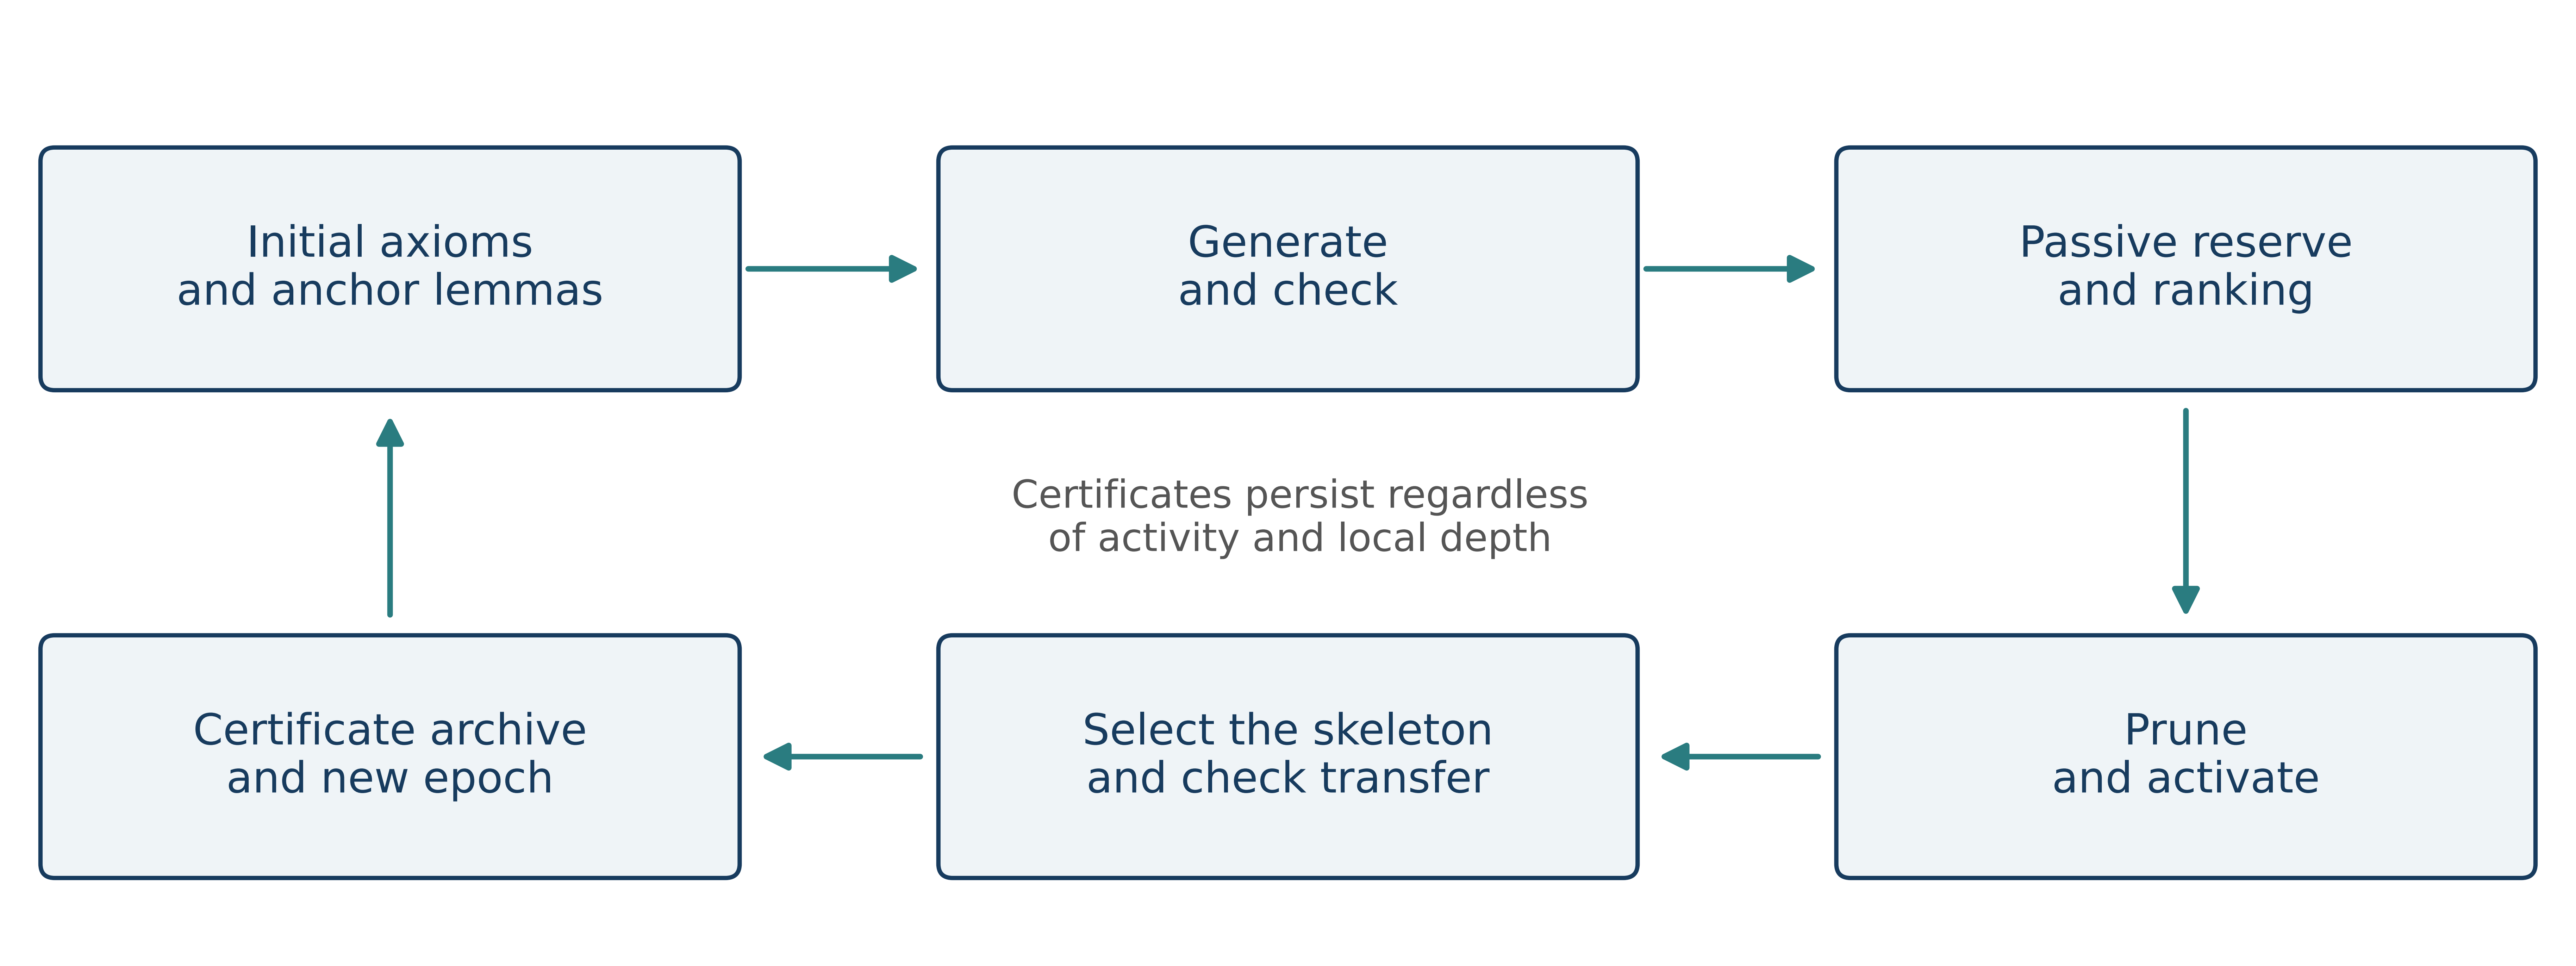
\includegraphics[width=\linewidth,height=.67\textheight,keepaspectratio]{Fig5.png}
\caption{Generation-based algorithm. Transfer and recovery require archive access; proof support persists independently of lemma activity. Certifying transfer does not establish optimal selection}\label{fig:5}
\end{figure}

\subsubsection*{C.1.3. Reviewing the anchor base}\label{c.1.3.-reviewing-the-anchor-base}
\addcontentsline{toc}{subsubsection}{C.1.3. Reviewing the anchor base}

At the end of an epoch, the policy retains lemmas as available compound steps for the next cycle. Selection can account for observed use, diversity of proof roles, record size, and expansion cost. Reserving part of the budget for little-used directions limits the risk that early popular lemmas monopolise growth.

Restarting search from a list of selected formulae does not, by itself, transfer knowledge completely. Every transferred lemma needs a certificate identifier, its original configuration, and a checkable chain to the initial axioms; the record keeps both the local generation number and a proof measure independent of restarts. This distinction prevents an artificial depth improvement through relabelling an expensive earlier lemma as an initial fact.

\subsection*{C.2. Optimising skeleton construction}\label{c.2.-optimising-skeleton-construction}
\addcontentsline{toc}{subsection}{C.2. Optimising skeleton construction}

\subsubsection*{C.2.1. Canonicalisation and reuse}\label{c.2.1.-canonicalisation-and-reuse}
\addcontentsline{toc}{subsubsection}{C.2.1. Canonicalisation and reuse}

We first canonicalise formulae, assigning one vertex to each declared normal form. Alternative proofs need not disappear: compact references can preserve several origins. Such references can support recovery, assessment of a lemma's role, or later checking without multiplying formula vertices.

Subsumption requires a checkable substitution witness. Replacing a formula by a more general schema requires an instance witness that preserves the substitution and every constraint; neither structural agreement nor graph-neighbourhood similarity supplies such a witness. Removing a candidate from active search therefore differs from quotienting the mathematical object.

\subsubsection*{C.2.2. Lemma utility}\label{c.2.2.-lemma-utility}
\addcontentsline{toc}{subsubsection}{C.2.2. Lemma utility}

An operational utility estimate must depend only on history available before the current decision. Internal signals include formula size, distinct observed derivations, productive uses, and expansion cost. Distinct hyperedges do not establish statistical independence of proofs, since shared ancestors can create strong dependence.

The implemented non-goal-directed ranking rewards rediscovery and penalises formula size. Let \(r_{d}\) count recorded rediscoveries and \(s(v)\) denote formula size in that implementation. We score candidates as follows:

\[\fitdisplay{U_{d}^{reuse}(v) = log(1 + r_{d}(v)) - logmax\{ 2,s(v)\}.}\]

This score supplies a specific heuristic that favours compact formulae and repeated derivations. Its terms use the implementation's rediscovery counter and size measure. They do not define mathematical value universally.

A small experiment with a pre-existing rule registry uses a different score. It assigns application \(e = (a,b \vdash c)\) the priority \(g_{d}(a) + g_{d}(b)\), where \(g_{d}\) counts earlier new consequences, and freezes that score when the application enters the queue. Its results therefore cannot support claims about the preceding formula or a more elaborate proposed utility family.

A generalised policy can also account for expected expansion cost and diversity of roles. Its weights, units, counter updates, and tie-breaking rule must precede the evaluation experiment. Using actual future productivity instead of a history-dependent estimate would introduce a hidden oracle.

\subsubsection*{C.2.3. Age-based pruning}\label{c.2.3.-age-based-pruning}
\addcontentsline{toc}{subsubsection}{C.2.3. Age-based pruning}

Age-based pruning, or rot-pruning, excludes little-used elements from future growth. The implementation protects initial axioms and anchors that transfer introduces at local depth zero; for active major premises it checks age since activation, absence of productive use, and absence of rediscovery, whereas passive candidates accumulate waiting age. Pruning removes entries from working indices and the queue, not materialised formulae or proofs.

This operation preserves accepted knowledge but can irreversibly restrict future search. An old candidate may gain value after a new premise appears. Past non-use therefore gives no certificate of future uselessness.

A separate policy must specify when to reactivate a vertex, whether a schedule, a context change, or a failed local search triggers the decision. Occasionally waking individual vertices does not ensure complete finite saturation; the scheduler must eventually process every available rule application. That guarantee concerns an unbounded continuation of a fair schedule and promises no completeness under a fixed budget.

\subsubsection*{C.2.4. Compressing proof dependencies}\label{c.2.4.-compressing-proof-dependencies}
\addcontentsline{toc}{subsubsection}{C.2.4. Compressing proof dependencies}

Sound compression replaces part of a concrete proof by a reference to a certified lemma. Expansion restores every jointly necessary premise. Since the archive can share subproofs, accounting must distinguish expanded-tree cost from the size of the stored directed acyclic graph.

Transitive reduction of an ordinary projection preserves paths but need not preserve derivability. Hyperedge \(\{ A,B\} \vdash C\) produces projected arc \(A \rightarrow C\) although \(A\) alone does not suffice; likewise, a projected cycle does not establish interchangeability of its vertices in every context. Component condensation and merging identical neighbourhoods therefore serve as structural diagnostics, not automatic proof compression.

\subsubsection*{C.2.5. Distinguishing policy versions}\label{c.2.5.-distinguishing-policy-versions}
\addcontentsline{toc}{subsubsection}{C.2.5. Distinguishing policy versions}

Table 9 separates each implemented mechanism from the guarantee it supports.

\begingroup
\small
\setlength{\tabcolsep}{3pt}
\renewcommand{\arraystretch}{1.13}

\begin{longtable}[]{@{}
  >{\raggedright\arraybackslash}p{(\linewidth - 4\tabcolsep) * \real{0.1836}}
  >{\raggedright\arraybackslash}p{(\linewidth - 4\tabcolsep) * \real{0.4327}}
  >{\raggedright\arraybackslash}p{(\linewidth - 4\tabcolsep) * \real{0.3837}}@{}}
\caption{Implemented policy mechanisms and the scope of their guarantees}\label{tab:9}\tabularnewline
\toprule\noalign{}
\begin{minipage}[b]{\linewidth}\raggedright
\textbf{Mechanism}
\end{minipage} & \begin{minipage}[b]{\linewidth}\raggedright
\textbf{Implemented operation}
\end{minipage} & \begin{minipage}[b]{\linewidth}\raggedright
\textbf{Limit of the claim}
\end{minipage} \\
\midrule\noalign{}
\endfirsthead
\toprule\noalign{}
\begin{minipage}[b]{\linewidth}\raggedright
\textbf{Mechanism}
\end{minipage} & \begin{minipage}[b]{\linewidth}\raggedright
\textbf{Implemented operation}
\end{minipage} & \begin{minipage}[b]{\linewidth}\raggedright
\textbf{Limit of the claim}
\end{minipage} \\
\midrule\noalign{}
\endhead
\bottomrule\noalign{}
\endlastfoot
Non-goal-directed utility & Rediscovery count and size penalty & Does not establish optimal lemma value \\
Utility on an exact registry & Past productive premise uses & Does not measure full generation cost \\
Age-based pruning & Limits working indices and queue & Does not preserve full closure \\
Earlier epoch transfer & Restarts from selected formulae & Does not maintain an end-to-end certificate archive \\
Graph skeletonisation & Prunes and reduces the projection & Does not establish semantic equivalence \\
Certified skeleton & Transfers anchors and replays certificates & Checked soundness does not imply optimality \\
Persistent queue and recipes & Resumes unfinished applications and jointly reactivates proof-fragment vertices & Effect depends on the regime \\
Selection by human lemmas & Chooses proven anchors that match a known set & Externally conditioned starting point, not automatic semantic assessment \\
Contextual transfer & Replaces some anchors through joint trial inferences with lemmas from another branch & Observed compatibility does not guarantee long-term utility \\
\end{longtable}

\endgroup

\subsection*{C.3. Contextual transfer between branches}\label{c.3.-contextual-transfer-between-branches}
\addcontentsline{toc}{subsection}{C.3. Contextual transfer between branches}

\subsubsection*{C.3.1. Recipient context and utility witnesses}\label{c.3.1.-recipient-context-and-utility-witnesses}
\addcontentsline{toc}{subsubsection}{C.3.1. Recipient context and utility witnesses}

Global ranking assigns a lemma one score regardless of its eventual companion premises. Two-premise inference makes that limitation consequential: two individually unproductive lemmas can jointly enable a new application. The method tests what a vertex contributes alongside a particular anchor base, rather than ranking it in isolation.

Trial witnesses record what candidate anchors jointly achieve in a recipient context. Let \(B\) denote the recipient branch's initial anchors and \(D\) the donor branch's proposals, with \(B \cap D = \varnothing\) and both sets containing proven lemmas. Freezing archive \(\Omega^{-}\) before trial expansion fixes the reference for new conclusions.

The main generator receives \(B \cup D\) and the original axioms. A separate observer records witnesses \(w = (R_{w},q_{w})\), where \(R_{w} \subseteq B \cup D\) denotes the non-axiomatic anchors that the recorded inference requires and \(q_{w} \notin V(\Omega^{-})\) denotes its conclusion. An independent checker validates every witness; for trial set \(\mathcal{W}\), define

\[\fitdisplay{\begin{matrix}
F(S) = \left| \{ q_{w}:\ w \in \mathcal{W},\ R_{w} \subseteq S\} \right|, \\
F_{cross}(S) = \left| \{ q_{w}:\ w \in \mathcal{W},\ R_{w} \subseteq S,\ R_{w} \cap B \neq \varnothing,\ R_{w} \cap D \neq \varnothing\} \right|.
\end{matrix}}\]

Both counts include each conclusion once, regardless of how many recorded proofs support it. The second counts conclusions with an observed derivation using anchors from both sources, without excluding a different proof that needs no exchange. These functions measure observed opportunities, not causal effects or complete counterfactual outcomes.

Even \(F\) can fail submodularity. If \(R_{w} = \{ a,b\}\) for the only witness, adding \(b\) to the empty set gives zero gain, whereas adding it to \(\{ a\}\) gives unit gain. The standard greedy-coverage guarantee therefore does not apply; selecting small bundles jointly reduces an obvious individual-ranking error without establishing optimality.

\subsubsection*{C.3.2. Selecting anchors under fixed quotas}\label{c.3.2.-selecting-anchors-under-fixed-quotas}
\addcontentsline{toc}{subsubsection}{C.3.2. Selecting anchors under fixed quotas}

The tested implementation uses \(|B| = 8\) and \(|D| \leq 16\). With enough proposals, selection must retain four old anchors and choose four new ones; starting from \(S = \varnothing\), it considers admissible one- or two-element additions \(U\) that respect those quotas. The first priority maximises

\[\fitdisplay{\frac{F_{cross}(S \cup U) - F_{cross}(S)}{|U|}.}\]

Tie-breaking first maximises the analogous per-element gain in \(F\). Further ties use absolute gains, smaller bundle size, and a fixed identifier order, and the algorithm repeats until all eight places fill. If the donor offers fewer than four lemmas, selection replaces only as many anchors as available proposals permit; the resulting rule defines a finite deterministic heuristic over recorded witnesses.

A worst-case count bounds the work of selecting from the finished catalogue. For \(p = |B \cup D|\), \(h = |\mathcal{W}|\), and quota \(k\), straightforward enumeration of singleton and pair additions requires at most \(O(kp^{2}h)\) membership checks when witness size remains bounded. This estimate excludes catalogue generation, unification, certificate checking, and subsequent generations, so the selector does not avoid the combinatorial explosion of the full space.

\subsubsection*{C.3.3. Running the two branches}\label{c.3.3.-running-the-two-branches}
\addcontentsline{toc}{subsubsection}{C.3.3. Running the two branches}

The initial base \(B\) draws only from initial archive \(\Omega_{0}\). With pool limit \(q\), selection merges the \(\lfloor q/3\rfloor\) shortest derived lemmas and the same number of most-used derived lemmas, removes duplicates, and fills remaining places in SHA-256 order from the initial state and identifier; usage counts refer to stored proof dependencies, not an external library, and size and identifier break ties in the first two lists. The initial pool uses \(q = 24\), whereas donor proposals use \(q = 16\).

An initial trial of at most three layers retains a bounded set of alternative dependency witnesses. Selection compares singleton and pair additions with each whole witness's missing anchors whenever those fit the remaining quota, maximising observed new conclusions per added anchor and then using absolute gain, smaller bundle size, and deterministic order. This procedure chooses eight initial anchors through a multilayer trial, not through exchange criterion \(F_{cross}\); the trial derives known intermediate formulae afresh instead of granting them as free extra premises.

The axiom branch then grows without anchors from \(\Omega_{0}\). Its new archived results supply donor pool \(D\) through the same short, frequently used, and pseudorandomly added lemma categories; one complete trial layer over \(B \cup D\) supplies the transfer catalogue, after which the recipient grows from the chosen eight anchors and original axioms. Each branch retains its state between generations, but transfer occurs only once, from donor to recipient, without a concurrent interacting search network or adaptive time allocation.

\begin{verbatim}
Check the common initial archive and choose eight anchors B.
Grow the axiom branch within the first share of the remaining budget.
Extract up to 16 new proven proposals D.
Run and check one layer over the union of B and D.
Choose four old and four new anchors through joint inferences.
Continue the skeleton branch up to the overall resource limit.
Count only prefixes with complete storage and checking.
\end{verbatim}

The branches share an archive, but the generator cannot use its contents as an unrestricted premise base. Every completed trial discovery enters the archive and contributes to costs and results, even when selection later rejects its anchors. A control with the same trial search and no transfer therefore matters: otherwise, apparent selection gains may merely reflect extra generation.

After common preparation, the donor receives half the remaining budget. Storing a completed layer can cross this internal boundary, but any overrun reduces the recipient's time rather than increasing the total allowance. Final results include only prefixes with complete commits before the overall budget expires, and accounting distinguishes full initial proof support and the common archive from the cardinality of the eight-anchor set (Fig. 6).

\begin{figure}[!htbp]
\centering
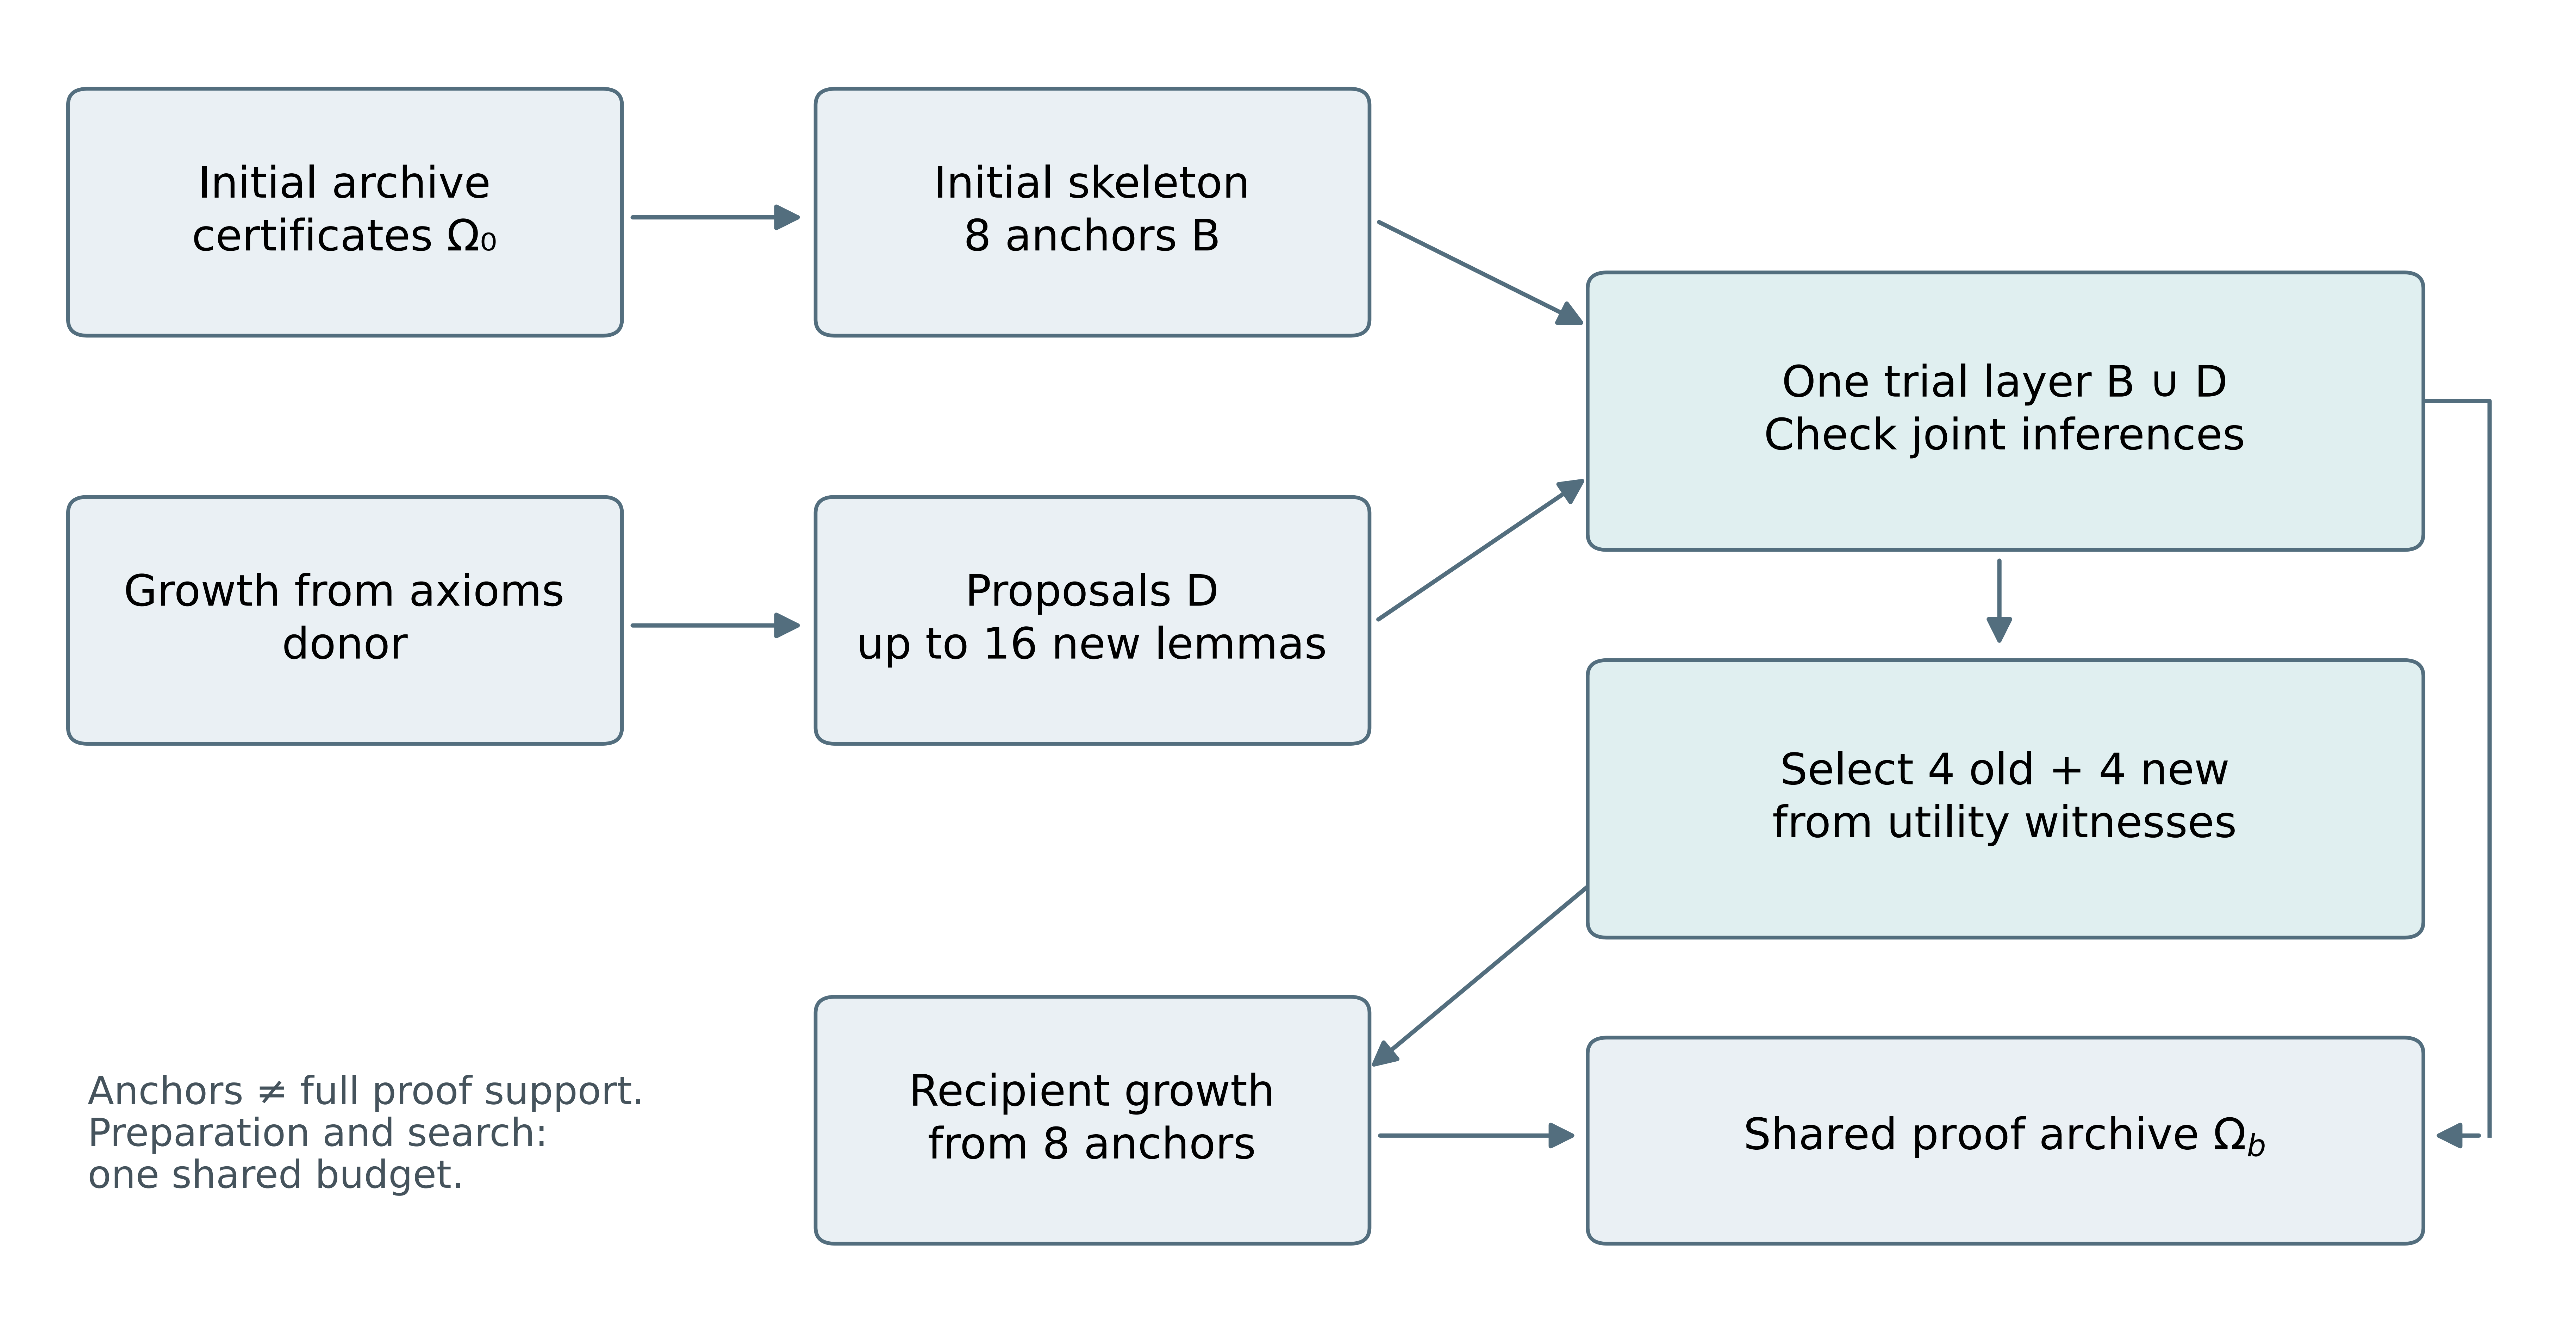
\includegraphics[width=\linewidth,height=.67\textheight,keepaspectratio]{Fig6.png}
\caption{One-way contextual transfer. The donor, preparatory trials, and recipient add to the common archive in sequence; trial discoveries persist regardless of anchor selection. Arrows show data flow, not concurrent branch execution}\label{fig:6}
\end{figure}

\section*{Appendix D. Complete experimental protocols}\label{appendix-d.-complete-experimental-protocols}
\addcontentsline{toc}{section}{Appendix D. Complete experimental protocols}

\subsection*{D.1. Experimental design}\label{d.1.-experimental-design}
\addcontentsline{toc}{subsection}{D.1. Experimental design}

\subsubsection*{D.1.1. Formal foundations and limits of comparison}\label{d.1.1.-formal-foundations-and-limits-of-comparison}
\addcontentsline{toc}{subsubsection}{D.1.1. Formal foundations and limits of comparison}

The main series starts from a classical propositional calculus. Its language contains \(\rightarrow ,\neg\), and its axiom system contains the following three schemata. These choices fix the propositional starting configuration:

\[\fitdisplay{\begin{matrix}
{ax}_{1}:A \rightarrow (B \rightarrow A), \\
{ax}_{2}:\lbrack A \rightarrow (B \rightarrow C)\rbrack \rightarrow \lbrack(A \rightarrow B) \rightarrow (A \rightarrow C)\rbrack, \\
{ax}_{3}:(\neg A \rightarrow \neg B) \rightarrow (B \rightarrow A),
\end{matrix}}\]

Schematic modus ponens renames the variables of the premises separately. The modal condition adds the axiom of normal logic K, \(\square(A \rightarrow B) \rightarrow (\square A \rightarrow \square B)\), and necessitation for theorems. These two configurations differ simultaneously in language, axioms, and rules, so they do not constitute a factorial experiment that identifies an independent causal effect of `logic in general'.

The bound \(L \in \{ 25,200\}\) counts vertices in the syntax tree of each canonical formula in storage. The separate KSP computational benchmark in Appendix G uses another axiomatisation and a leaf metric. Its figures therefore remain separate from the main series.

Every new result carries a certificate back to the original axioms. An independent checker implements its own canonicalisation, unification with an occurs check, and rule checks, without importing the generator's code for these operations. It checks one first proof per vertex in storage, not the completeness of all alternative derivations.

The unit of replication follows the experimental design. In growth experiments it comprises a trajectory with a random initial scheduling state; in continuation experiments it comprises a common source archive with paired comparisons of anchor-selection methods. Thousands of formulae within one trajectory do not count as independent observations.

\subsubsection*{D.1.2. Screening and confirmation of construction policies}\label{d.1.2.-screening-and-confirmation-of-construction-policies}
\addcontentsline{toc}{subsubsection}{D.1.2. Screening and confirmation of construction policies}

The screening compares seven selection variants: syntactic-feature coverage, random selection, structural diversity, jointly applicable premises, diversity of compatibility profiles, and two combinations of these features. Each variant switches two mechanisms on or off: a persistent queue of unfinished inference opportunities and concrete proof recipes, yielding 28 conditions. A recipe rechecks a proof fragment from storage and jointly reactivates its conclusion and internal premises; the operation itself produces no new conclusion, leaving new consequences to the common generator, and supplies no generalised learnt rule.

The screening stage contains \(28 \times 2 \times 2 \times 3 = 336\) trajectories. Within each block, every condition receives a copy of one state with a certificate; a rule from the protocol chooses the first prefix in storage with two epochs without globally new formulae, or the last prefix within budget if no stagnation occurs, and records the actual stagnation status. The common source requires construction only once, but each complete pipeline incurs its construction cost in the comparison; conditions exchange no new discoveries.

The selection rule identifies four finalists after checks of all 336 trajectories. It ranks variants by the worst of their four stratum-specific median log-gains, and the protocol specifies tie-breaking and control conditions in advance. Random selection with a queue and recipes wins this screening and then faces the original coverage policy, random selection without either mechanism, and random selection with recipes alone.

The `random' variant in the first series includes short probe expansions and reactivation during stagnation, whereas the original coverage policy includes neither. It therefore supplies an enhanced random control, not a pure random queue. It also differs from the random choice of eight anchors in the second series.

Confirmation contains \(4 \times 2 \times 2 \times 8 = 128\) trajectories with scheduling states 1301--1308, which did not appear during screening. Every condition starts from the original axioms and an empty derived archive, with 32 anchors, up to 32 new activations per main-generator layer, four generations per epoch, at most 128 epochs, and safeguards of 50 000 local and 100 000 archive vertices. Up to eight activation slots go to the oldest candidates and the remainder follow utility; this quota does not cap the total active set. Auxiliary recovery windows run one layer without an activation-count limit but with a cap of 2 048 local vertices. Construction budgets allow 120 CPU-seconds at \(L = 25\) and 360 at \(L = 200\), including selection, probes, queue maintenance, checking, and storage; completions beyond budget remain available for diagnosis but earn no credit within budget.

The primary outcome depends on the size bound. At \(L = 25\) it measures non-axiomatic coverage of the exact \(H_{4}\); at \(L = 200\) it measures the increase in MP-born formulae between the last admissible prefix and the prefix at two thirds of the budget. The latter estimates late productivity from prefixes rather than the exact event rate during the final third of elapsed time; modal necessitation results receive separate counts and do not replace MP productivity.

Full superiority of the screening winner requires four conditions simultaneously against both fixed controls in all four strata. All eight paired differences must exceed zero, the ratio of means must satisfy \((1 + {\overline{Y}}_{1})/(1 + {\overline{Y}}_{0}) \geq 1.10\), the one-sided lower bound for the mean log-gain must exceed zero, and the comparison must pass Holm's procedure. The analysis uses 20 000 paired bootstrap resamples with a Bonferroni correction for eight comparisons and applies exhaustive sign flips to

\[\fitdisplay{g_{i} = log(1 + Y_{1i}) - log(1 + Y_{0i}).}\]

The sign-flip test concerns log-gains, not raw outcome differences. It requires symmetry and exchangeability of the \(g_{i}\) themselves under the null hypothesis. Consequently, it offers no unconditional proof of transfer to new logics.

\textbf{Recovery of an incomplete block}

The original confirmation run completed 31 full blocks out of 32. In the propositional block with \(L = 25\) and state 1308, the random control stopped after the code failed to handle a CPU-timer exception during timer shutdown. The original audit remains incomplete and counts 124 trajectories, excluding the three successful conditions in the incomplete block from separate use.

Recovery reran all four conditions in that block once after a timer-shutdown fix, with the same parameters, order, and scheduling state. The finalists did not change, and a separate report combines the 124 earlier trajectories that passed checking with the four recovery trajectories while preserving the original files and the old audit's negative status. This disclosure records a change of execution version, not `successful completion' of the unchanged original run; sensitivity analysis excludes the recovery block alongside the main estimate.

\subsubsection*{D.1.3. Human theorem sets and anchor selection}\label{d.1.3.-human-theorem-sets-and-anchor-selection}
\addcontentsline{toc}{subsubsection}{D.1.3. Human theorem sets and anchor selection}

The study uses a pinned version of the \path{set.mm} database \citep{MetamathSetMMPinned}, not its changing current library. The first comparison selects closed propositional theorems from the primitive prefix before equivalence syntax, excludes essential hypotheses and distinct-variable restrictions, and caps conclusion size at 25; removing original axiom schemata and duplicates under variable renaming leaves 47 statements. The first series compares against this set only after the search finishes.

The second experiment turns those 47 formulae into an open set for choosing anchors from human theorems. They therefore no longer supply an independent control set; a separate extraction from the same pinned library yields 108 evaluation statements after removing exact duplicates and formulae with substitution links to the first set. Those statements form 106 substitution families, and all conclusions contain between 5 and 25 syntax-tree vertices despite an extraction allowance up to 200.

Neither anchor selection nor the generator receives the 108 evaluation formulae. Nevertheless, these public statements come from one library, and their proof dependencies overlap with those of the first set; truth-table checks establish propositional correctness, not a replay of the human Metamath proofs. The study does not check intermediate-formula sizes in those proofs, so failure to match does not automatically implicate the growth policy, and this propositional set offers no full external benchmark for modal logic.

\subsubsection*{D.1.4. Direct continuation from a fixed number of anchors}\label{d.1.4.-direct-continuation-from-a-fixed-number-of-anchors}
\addcontentsline{toc}{subsubsection}{D.1.4. Direct continuation from a fixed number of anchors}

The second experiment asks a separate question about the utility of the starting representation. It uses 16 propositional archives with certificates from the original coverage policy in the confirmation series, eight at each size bound, including one source from the recovery block. The winner of the first series did \textbf{not} produce these archives, so the experiment does not test a combined `best growth--best skeleton' pipeline.

Five methods select anchors from each common archive. The following table specifies their starting representations and distinguishes the axiom-only control. This distinction keeps the eight-anchor variants separate from the baseline that adds no anchors (Table 10).

\begingroup
\small
\setlength{\tabcolsep}{3pt}
\renewcommand{\arraystretch}{1.13}

\begin{longtable}[]{@{}
  >{\raggedright\arraybackslash}p{(\linewidth - 2\tabcolsep) * \real{0.1681}}
  >{\raggedright\arraybackslash}p{(\linewidth - 2\tabcolsep) * \real{0.8319}}@{}}
\caption{Starting representations for the five direct-continuation controls}\label{tab:10}\tabularnewline
\toprule\noalign{}
\begin{minipage}[b]{\linewidth}\raggedright
\textbf{Variant}
\end{minipage} & \begin{minipage}[b]{\linewidth}\raggedright
\textbf{Starting representation}
\end{minipage} \\
\midrule\noalign{}
\endfirsthead
\toprule\noalign{}
\begin{minipage}[b]{\linewidth}\raggedright
\textbf{Variant}
\end{minipage} & \begin{minipage}[b]{\linewidth}\raggedright
\textbf{Starting representation}
\end{minipage} \\
\midrule\noalign{}
\endhead
\bottomrule\noalign{}
\endlastfoot
Feature coverage & Eight formulae that a greedy rule chooses by syntactic-coverage gain per byte of new proof support \\
Random & Eight formulae from the entire common derived archive, following hash order over the initial state and identifier \\
Shortest & Eight formulae of minimum size, with a fixed tie-breaking rule \\
Human & Eight formulae whose certificates pass checking and that exactly match the open set of 47, shortest first and then by identifier \\
Axiomatic & Only the three original axiom schemata, without additional anchors \\
\end{longtable}

\endgroup

All automatic variants share the entire common derived archive as their candidate pool. The human variant uses only formulae whose proofs already occur in that archive and imports neither new axioms nor ready-made human proofs. Each source offers 11--14 admissible matches from which to choose eight.

The coverage criterion combines shallow syntax with proof-use information. Let \(\mathcal{F}(v)\) contain shallow features of the root, subformulae, antecedent, and consequent; let \(u(v)\) count direct uses and let \(w(v)\) estimate first-proof tree size with a cap of \(10^{9}\). These quantities define

\[\fitdisplay{q(v) = (1 + log(1 + u(v)))(1 + logw(v)),}\]

\[\fitdisplay{F(S) = \sum_{f}^{}\max_{\substack{v \in S \\ f \in \mathcal{F}(v)}}q(v),\quad\quad max\varnothing = 0.}\]

Each selection step maximises \(\Delta F/max\{ 1,\Delta B\}\). Here \(\Delta B\) counts bytes of proof-support records that the current set does not yet include, and the denominator's lower bound handles candidates that already occur among support vertices. Cost depends on the current \(S\), so the study claims neither optimality nor a standard approximation factor for this ratio; this starting-anchor criterion also differs from the generator's operational utility, which uses repeated derivations.

Every variant retains the original axioms and checks and stores support vertices without feeding them to the generator as additional starting lemmas. Continuation uses one fixed stateful generator with up to 32 new activations per layer, including up to eight oldest candidates and utility choices for the remainder according to repeated derivations and size; age pruning removes active major premises and passive candidates after two layers but protects original axioms and starting anchors. Limits allow at most 128 complete layers, 50 000 local, and 100 000 archive vertices, and the procedure uses no target queries, backward search, proof recipes, or external model.

The continuation series runs five conditions on each common source, giving \(16 \times 5 = 80\) trajectories. Continuation states 2301--2308 and condition order follow choices from before execution; the primary outcome uses \(N_{30}\) and the 10-second checkpoint supplies a secondary outcome. Credit goes to the last prefix that passes internal checks and finishes storage by 30 CPU-seconds, and an independent auditor then checks that prefix; incomplete generations and storage commits beyond budget receive no credit.

The continuation budget covers loading the common archive, replaying its certificate, anchor selection, support construction, generation, checking, and storage. Even the axiom-only control loads the common archive to count novelty correctly, a shared measurement cost rather than the minimum cost of a standalone start from axioms. We account separately for the historical cost of constructing the source, so this experiment measures conditional continuation utility, not the return on the complete pipeline.

The six primary comparisons test coverage, shortest, and human anchors against random anchors at two values of \(L\). The analysis uses 20 000 paired bootstrap resamples, a one-sided level of \(0.05/6\), and Holm's procedure for exhaustive sign flips of paired log-gains \(g_{i}\); comparisons with the axiom-only control and human matches remain secondary and descriptive. The hypotheses concern eight source blocks per stratum, for which eight non-zero differences permit a minimum one-sided \(p\)-value of \(1/256.\)

\subsubsection*{D.1.5. Context-transfer test}\label{d.1.5.-context-transfer-test}
\addcontentsline{toc}{subsubsection}{D.1.5. Context-transfer test}

The third experiment retains the direct design but combines axiomatic and skeleton branches in place of a single skeleton trajectory. Every condition shares the same source archive, and the outcome counts the union of new canonical formulae outside that archive without charging its historical construction cost again to the continuation budget. Six conditions separate the contributions of budget splitting, branch diversity, probing, and transfer (Table 11).

\begingroup
\small
\setlength{\tabcolsep}{3pt}
\renewcommand{\arraystretch}{1.13}

\begin{longtable}[]{@{}
  >{\raggedright\arraybackslash}p{(\linewidth - 4\tabcolsep) * \real{0.1461}}
  >{\raggedright\arraybackslash}p{(\linewidth - 4\tabcolsep) * \real{0.4757}}
  >{\raggedright\arraybackslash}p{(\linewidth - 4\tabcolsep) * \real{0.3782}}@{}}
\caption{Conditions and controlled differences in the context-transfer test}\label{tab:11}\tabularnewline
\toprule\noalign{}
\begin{minipage}[b]{\linewidth}\raggedright
\textbf{Code}
\end{minipage} & \begin{minipage}[b]{\linewidth}\raggedright
\textbf{Condition}
\end{minipage} & \begin{minipage}[b]{\linewidth}\raggedright
\textbf{Difference under test}
\end{minipage} \\
\midrule\noalign{}
\endfirsthead
\toprule\noalign{}
\begin{minipage}[b]{\linewidth}\raggedright
\textbf{Code}
\end{minipage} & \begin{minipage}[b]{\linewidth}\raggedright
\textbf{Condition}
\end{minipage} & \begin{minipage}[b]{\linewidth}\raggedright
\textbf{Difference under test}
\end{minipage} \\
\midrule\noalign{}
\endhead
\bottomrule\noalign{}
\endlastfoot
A & One axiomatic growth run & Main control without skeleton anchors \\
A+A & Two axiomatic growth runs with different initial states & Splitting the computational budget itself \\
A+S & Axiomatic and skeleton branches without exchange & Diversity of two starting representations \\
Probe & A+S plus a probe layer, without anchor replacement & Utility of additional probe inferences \\
Random & The same probe layer, with random anchor replacement & Transfer itself under a fixed quota \\
Context & The same probe layer, with context-based replacement & The proposed selection criterion \\
\end{longtable}

\endgroup

The initial three-layer probe uses width 32, retains up to four witnesses per formula and at most 20 000 records, and allows 8 192 local vertices and two CPU-seconds. The one-layer exchange probe caps local vertices at 4 096 and CPU time at one second; these costs consume the common budget, and an incomplete probe contributes only results that pass all checks, with probe completion entering a separate check criterion. Exchange variants replace four of eight anchors whenever the donor offers at least four lemmas, whereas every condition retains the original axioms.

The short series contains four development sources and four other sources to test how the unchanged algorithm transfers. Each group supplies two sources per \(L\) and six conditions per source, totalling 48 trajectories with a 20-CPU-second budget; all sources belong to the existing utility study, but development of this policy did not use the second group of four. Earlier work on the first group examined one-layer joint scoring and multilayer scores, and their failures remain part of the development history, so this short transfer series does not confirm transfer to independent mathematical theories.

Before the long series, the protocol set a descriptive rule for proceeding. Context must outperform A+S, Probe, and random replacement in at least three of four source blocks for each comparison, mean new-formula counts must exceed A and A+A at each \(L\), and all exchange probes must finish. This rule grants access to the next budget rather than testing statistical significance; two sources per stratum cannot support a persuasive conclusion about the population mean.

The long series uses four further sources that did not contribute to policy development, two at \(L = 25\) and two at \(L = 200\). Each source runs all six conditions at 60 and 180 CPU-seconds, adding 48 trajectories with unchanged generation and selection code; only resource safeguards increase, to 1 024 generations, 250 000 local, and 500 000 archive vertices. A soft process-memory threshold of 4 GiB supplies a program-level safeguard rather than a hard operating-system quota, and reaching any safeguard triggers a record rather than a claim of saturation.

The 60- and 180-second budgets define independent runs because the donor-to-recipient transition depends on the final budget. A prefix of the longer axiomatic stage cannot substitute for a separate 60-second experiment; all long-series conditions run locally with two concurrent processes and a separate CPU-time limit for each process. Absolute speeds therefore do not enter direct comparisons with the cluster's 30-second series, and we account separately for the later independent audit\textquotesingle s cost.

\subsubsection*{D.1.6. Protocol for testing the library and search activity}\label{d.1.6.-protocol-for-testing-the-library-and-search-activity}
\addcontentsline{toc}{subsubsection}{D.1.6. Protocol for testing the library and search activity}

The final continuous series tests the architecture without a pre-existing source: \(\Omega_{0}\) contains only the original axioms. It covers three strata: propositional calculus at \(L = 25\), the same calculus at \(L = 200\), and modal logic K at \(L = 25\); no condition collects complete alternative provenance, whereas every condition stores and checks the first proof of each canonical formula. All variants share one generator, identical canonicalisation, no subsumption, and an append-only log, so within-series comparisons do not conflate policy changes with a switch from full-prefix storage to incremental storage.

The initial test used two tie-breaking states and 18 runs of 10 CPU-seconds, comparing the previous policy, revised activity control, and an active fragment library. The subsequent protocol froze an expanded series of 48 runs on four new states, with checkpoints at 10, 30, and 60 CPU-seconds, and added a passive-library variant. Run order and parameters preceded all expanded-series results, and the three checkpoints belong to one trajectory rather than three independent replicates (Table 12).

\begingroup
\small
\setlength{\tabcolsep}{3pt}
\renewcommand{\arraystretch}{1.13}

\begin{longtable}[]{@{}
  >{\raggedright\arraybackslash}p{(\linewidth - 4\tabcolsep) * \real{0.1292}}
  >{\raggedright\arraybackslash}p{(\linewidth - 4\tabcolsep) * \real{0.5300}}
  >{\raggedright\arraybackslash}p{(\linewidth - 4\tabcolsep) * \real{0.3408}}@{}}
\caption{Search activity and proof-library roles in the pilot and longer-series protocol}\label{tab:12}\tabularnewline
\toprule\noalign{}
\begin{minipage}[b]{\linewidth}\raggedright
\textbf{Code}
\end{minipage} & \begin{minipage}[b]{\linewidth}\raggedright
\textbf{Search state}
\end{minipage} & \begin{minipage}[b]{\linewidth}\raggedright
\textbf{Proof library}
\end{minipage} \\
\midrule\noalign{}
\endfirsthead
\toprule\noalign{}
\begin{minipage}[b]{\linewidth}\raggedright
\textbf{Code}
\end{minipage} & \begin{minipage}[b]{\linewidth}\raggedright
\textbf{Search state}
\end{minipage} & \begin{minipage}[b]{\linewidth}\raggedright
\textbf{Proof library}
\end{minipage} \\
\midrule\noalign{}
\endhead
\bottomrule\noalign{}
\endlastfoot
P & Previous age pruning, without the new cap on the total active set & None \\
O & Bounded activity and reversible deactivation & None \\
OA & As O, with finite retention and return of fragments that selection chooses & Influences search premises \\
OB & Exactly the search policy of O & Storage and scoring without search changes \\
\end{longtable}

\endgroup

Selection width totals 32 formulae per layer. O, OA, and OB cap active derived formulae at 128 and passive candidates at 4 096, exclude original axioms from the 128 active slots, use active and passive retention periods of six and four epochs, delay repeated return by two epochs, and allow eight rediscovery-driven returns per layer. The library holds at most four fragments; every four epochs, selection examines the latest 128 first proofs and at most 16 candidates, with a separate library-retention period of six epochs, and these values do not depend on the long block's results.

Shared safeguards cap local formulae at 500 000 and epochs at 4 096 and set a soft threshold of 1.5 GiB for peak process memory. Memory checks occur between layers rather than through a hard system limit, and trajectories that reach a safeguard remain in the comparison with their stopping reason. Only layers that complete checking and storage before the budget checkpoint earn credit; this series incurs no historical source-construction cost, and interpreter startup and the final independent audit remain outside the algorithmic CPU budget.

The primary measure uses \(N_{60}\) relative to the original axioms. Secondary measures cover \(N_{10}\), \(N_{30}\), active-set, support, and archive sizes, memory, log size, stage costs, and later fragment use; separate comparisons examine O versus P, OA versus O, OB versus O, and OA versus OB. O versus P tests the whole change package rather than the causal effect of any one retention period or quota, whereas OA and OB distinguish library maintenance from its effect on search trajectories; requiring positive paired differences on all four states within a stratum gives a descriptive rule for consistently positive differences, not a test of statistical significance.

\section*{Appendix E. Earlier results}\label{appendix-e.-earlier-results}
\addcontentsline{toc}{section}{Appendix E. Earlier results}

\subsection*{E.1. Results}\label{e.1.-results}
\addcontentsline{toc}{subsection}{E.1. Results}

\subsubsection*{E.1.1. Scale of generational growth}\label{e.1.1.-scale-of-generational-growth}
\addcontentsline{toc}{subsubsection}{E.1.1. Scale of generational growth}

A preliminary exact calculation of the H14 configuration illustrates the resource motivation. It records complete provenance and uses no subsumption. Its performance figures therefore do not enter a unified comparison with the main series (Table 13).

\begingroup
\small
\setlength{\tabcolsep}{3pt}
\renewcommand{\arraystretch}{1.13}

\begin{longtable}[]{@{}
  >{\raggedright\arraybackslash}p{(\linewidth - 4\tabcolsep) * \real{0.2924}}
  >{\raggedleft\arraybackslash}p{(\linewidth - 4\tabcolsep) * \real{0.2924}}
  >{\raggedleft\arraybackslash}p{(\linewidth - 4\tabcolsep) * \real{0.4153}}@{}}
\caption{Exact new and cumulative schema counts in the preliminary H14 calculation}\label{tab:13}\tabularnewline
\toprule\noalign{}
\begin{minipage}[b]{\linewidth}\raggedright
\textbf{Depth}
\end{minipage} & \begin{minipage}[b]{\linewidth}\raggedleft
\textbf{New schemata}
\end{minipage} & \begin{minipage}[b]{\linewidth}\raggedleft
\textbf{Cumulative schemata}
\end{minipage} \\
\midrule\noalign{}
\endfirsthead
\toprule\noalign{}
\begin{minipage}[b]{\linewidth}\raggedright
\textbf{Depth}
\end{minipage} & \begin{minipage}[b]{\linewidth}\raggedleft
\textbf{New schemata}
\end{minipage} & \begin{minipage}[b]{\linewidth}\raggedleft
\textbf{Cumulative schemata}
\end{minipage} \\
\midrule\noalign{}
\endhead
\bottomrule\noalign{}
\endlastfoot
0 & 13 & 13 \\
1 & 107 & 120 \\
2 & 4 917 & 5 037 \\
3 & 3 168 903 & 3 173 940 \\
\end{longtable}

\endgroup

At depth 3, the calculation recorded 14 783 595 modus-ponens attempts and 4 365 522 hyperedges. The size limit never triggered, and the analysis does not substitute the original report's finalisation time for total construction time. These four endpoints show a sharp increase in the materialised result but do not determine an asymptotic law for schema growth.

\subsubsection*{E.1.2. Policy confirmation: improvement depends on the regime}\label{e.1.2.-policy-confirmation-improvement-depends-on-the-regime}
\addcontentsline{toc}{subsubsection}{E.1.2. Policy confirmation: improvement depends on the regime}

The panel after recovery contains 128 trajectories that passed checking. The screening's winning combination passes six of eight comparisons under the overall criterion from the frozen protocol but fails both comparisons with the enhanced random control at \(L = 200\). The result therefore demonstrates conditional trade-offs, not universal superiority (Table 14).

\begingroup
\small
\setlength{\tabcolsep}{3pt}
\renewcommand{\arraystretch}{1.13}

\begin{longtable}[]{@{}
  >{\raggedright\arraybackslash}p{(\linewidth - 10\tabcolsep) * \real{0.1450}}
  >{\raggedright\arraybackslash}p{(\linewidth - 10\tabcolsep) * \real{0.1712}}
  >{\raggedleft\arraybackslash}p{(\linewidth - 10\tabcolsep) * \real{0.1623}}
  >{\raggedleft\arraybackslash}p{(\linewidth - 10\tabcolsep) * \real{0.1450}}
  >{\raggedleft\arraybackslash}p{(\linewidth - 10\tabcolsep) * \real{0.2143}}
  >{\raggedright\arraybackslash}p{(\linewidth - 10\tabcolsep) * \real{0.1623}}@{}}
\caption{Confirmatory policy outcomes by logic, formula-size bound, and frozen success criterion}\label{tab:14}\tabularnewline
\toprule\noalign{}
\begin{minipage}[b]{\linewidth}\raggedright
\textbf{Logic, bound}
\end{minipage} & \begin{minipage}[b]{\linewidth}\raggedright
\textbf{Primary outcome}
\end{minipage} & \begin{minipage}[b]{\linewidth}\raggedleft
\textbf{Random control}
\end{minipage} & \begin{minipage}[b]{\linewidth}\raggedleft
\textbf{Combi\-nation}
\end{minipage} & \begin{minipage}[b]{\linewidth}\raggedleft
\textbf{Ratio of means with} \(+ 1\)
\end{minipage} & \begin{minipage}[b]{\linewidth}\raggedright
\textbf{Full criterion}
\end{minipage} \\
\midrule\noalign{}
\endfirsthead
\toprule\noalign{}
\begin{minipage}[b]{\linewidth}\raggedright
\textbf{Logic, bound}
\end{minipage} & \begin{minipage}[b]{\linewidth}\raggedright
\textbf{Primary outcome}
\end{minipage} & \begin{minipage}[b]{\linewidth}\raggedleft
\textbf{Random control}
\end{minipage} & \begin{minipage}[b]{\linewidth}\raggedleft
\textbf{Combi\-nation}
\end{minipage} & \begin{minipage}[b]{\linewidth}\raggedleft
\textbf{Ratio of means with} \(+ 1\)
\end{minipage} & \begin{minipage}[b]{\linewidth}\raggedright
\textbf{Full criterion}
\end{minipage} \\
\midrule\noalign{}
\endhead
\bottomrule\noalign{}
\endlastfoot
Prop., 25 & \(H_{4}\) coverage & 1 456.75 & 1 752.00 & 1.203 & Pass \\
Modal, 25 & \(H_{4}\) coverage & 2 124.50 & 2 559.88 & 1.205 & Pass \\
Prop., 200 & Late MP novelty & 17 655.50 & 19 877.50 & 1.126 & Fail \\
Modal, 200 & Late MP novelty & 16 750.25 & 17 245.13 & 1.030 & Fail \\
\end{longtable}

\endgroup

At \(L = 25\), all eight paired differences exceed zero in each logic. At \(L = 200\), seven and four differences respectively exceed zero, and one-sided \(p\)-values of \(0.02734\) and \(0.17969\) fail Holm's procedure. The propositional regime makes the distinction especially clear: its mean gain exceeds 10\%, yet it fails the joint confirmation conditions, and the analysis does not choose another winning policy after inspecting these results (Fig. 7).

\begin{figure}[!htbp]
\centering
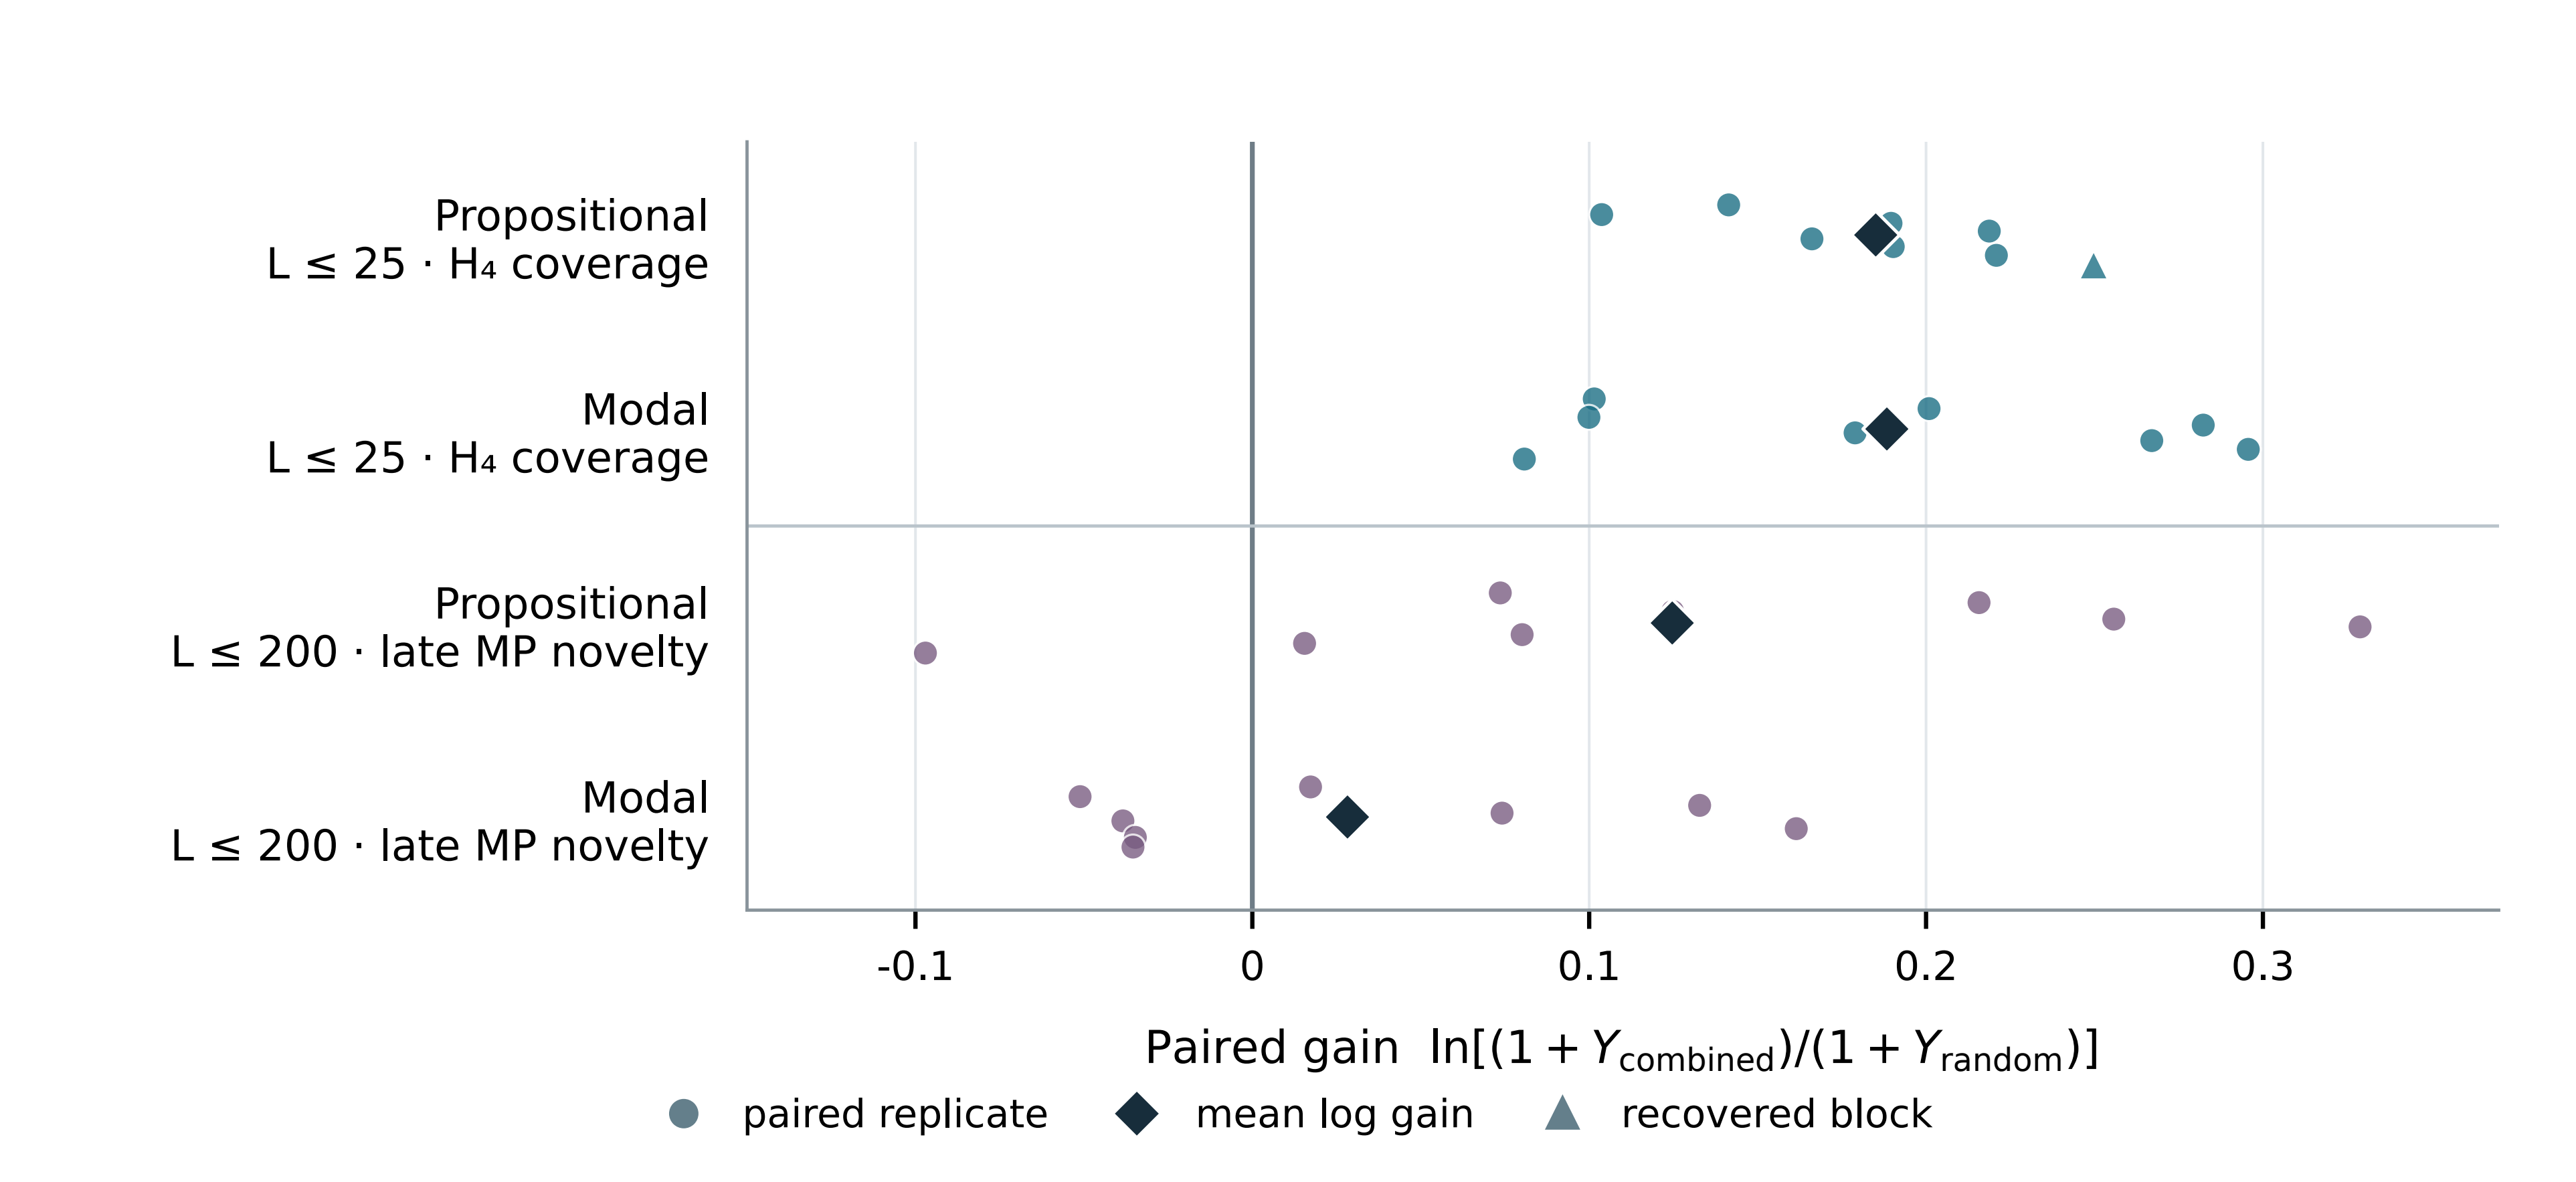
\includegraphics[width=\linewidth,height=.67\textheight,keepaspectratio]{Fig7.png}
\caption{Paired log-gains of the combination over the enhanced random control. Points mark eight replicates, diamonds mark mean log-gains, and the triangle marks the recovery block. At bound 25, the outcome measures exact-benchmark coverage; at 200, it measures late MP novelty. The plot omits intervals, and a positive mean does not imply a pass under the overall criterion}\label{fig:7}
\end{figure}

At \(L = 200\), the original coverage policy produces zero late MP novelty in every replicate of both logics. An advantage over that control shows escape from a specific stagnation regime but provides substantially less information than comparison with the already productive enhanced random variant. This distinction rules out treating every observed escape from stagnation as evidence of an optimal skeleton.

\subsubsection*{E.1.3. Finite-benchmark coverage and human lemmas}\label{e.1.3.-finite-benchmark-coverage-and-human-lemmas}
\addcontentsline{toc}{subsubsection}{E.1.3. Finite-benchmark coverage and human lemmas}

The following table concerns eight propositional confirmation replicates at \(L = 25\). The non-axiomatic part of \(H_{4}\) contains 2 828 schemata. Active coverage counts only anchors, not proof-support vertices, and therefore measures a narrower set than archive coverage (Table 15).

\begingroup
\small
\setlength{\tabcolsep}{3pt}
\renewcommand{\arraystretch}{1.13}

\begin{longtable}[]{@{}
  >{\raggedright\arraybackslash}p{(\linewidth - 8\tabcolsep) * \real{0.2274}}
  >{\raggedleft\arraybackslash}p{(\linewidth - 8\tabcolsep) * \real{0.1017}}
  >{\raggedleft\arraybackslash}p{(\linewidth - 8\tabcolsep) * \real{0.2115}}
  >{\raggedleft\arraybackslash}p{(\linewidth - 8\tabcolsep) * \real{0.2531}}
  >{\raggedleft\arraybackslash}p{(\linewidth - 8\tabcolsep) * \real{0.2062}}@{}}
\caption{Finite-benchmark and human-lemma coverage in propositional confirmation at size 25}\label{tab:15}\tabularnewline
\toprule\noalign{}
\begin{minipage}[b]{\linewidth}\raggedright
\textbf{Policy}
\end{minipage} & \begin{minipage}[b]{\linewidth}\raggedleft
\(H_{4}\) \textbf{coverage}
\end{minipage} & \begin{minipage}[b]{\linewidth}\raggedleft
\textbf{Exact archive matches out of 47}
\end{minipage} & \begin{minipage}[b]{\linewidth}\raggedleft
\textbf{Archive substitution coverage out of 47}
\end{minipage} & \begin{minipage}[b]{\linewidth}\raggedleft
\textbf{Exact anchor matches out of 47}
\end{minipage} \\
\midrule\noalign{}
\endfirsthead
\toprule\noalign{}
\begin{minipage}[b]{\linewidth}\raggedright
\textbf{Policy}
\end{minipage} & \begin{minipage}[b]{\linewidth}\raggedleft
\(H_{4}\) \textbf{coverage}
\end{minipage} & \begin{minipage}[b]{\linewidth}\raggedleft
\textbf{Exact archive matches out of 47}
\end{minipage} & \begin{minipage}[b]{\linewidth}\raggedleft
\textbf{Archive substitution coverage out of 47}
\end{minipage} & \begin{minipage}[b]{\linewidth}\raggedleft
\textbf{Exact anchor matches out of 47}
\end{minipage} \\
\midrule\noalign{}
\endhead
\bottomrule\noalign{}
\endlastfoot
Coverage, without queue or recipes & 919.63 & 13.13 & 13.13 & 7.13 \\
Random control & 1 456.75 & 11.75 & 12.00 & 0.38 \\
Random with recipes & 1 673.50 & 12.13 & 12.63 & 0.75 \\
Random with queue and recipes & 1 752.00 & 12.63 & 13.13 & 1.50 \\
\end{longtable}

\endgroup

The original axioms match none of this set, so confirmation-stage matches add something new to the axiomatic start. Substitution coverage includes exact coverage but retains a separate assessment role. Archive coverage likewise differs from retention of matches among active anchors.

At \(L = 200\), the original and combined variants yield respectively 12.13 and 13.25 exact archive matches, but 7.25 and 3.00 matches in the active skeleton. The human set still contains the same short conclusions, whereas the larger \(L\) permits different intermediate schemata. Means from the two bounds therefore remain separate.

Higher coverage of the finite schematic benchmark accompanies fewer human matches among anchors than the original selection policy retains. This pattern reveals a disagreement between criteria through post hoc diagnosis. It supplies neither independent confirmation of quality nor a comparison with all of Metamath.

\subsubsection*{E.1.4. Anchor utility under identical direct continuation}\label{e.1.4.-anchor-utility-under-identical-direct-continuation}
\addcontentsline{toc}{subsubsection}{E.1.4. Anchor utility under identical direct continuation}

All 80 trajectories in the second series passed independent certificate replay. The table reports mean new canonical formulae over 30 CPU-seconds. Novelty uses the \textbf{entire} common source archive as its reference, not merely the starting anchors (Table 16).

\begingroup
\small
\setlength{\tabcolsep}{3pt}
\renewcommand{\arraystretch}{1.13}

\begin{longtable}[]{@{}
  >{\raggedright\arraybackslash}p{(\linewidth - 4\tabcolsep) * \real{0.3831}}
  >{\raggedleft\arraybackslash}p{(\linewidth - 4\tabcolsep) * \real{0.3084}}
  >{\raggedleft\arraybackslash}p{(\linewidth - 4\tabcolsep) * \real{0.3084}}@{}}
\caption{Mean new canonical formulae under identical 30-CPU-second direct continuation}\label{tab:16}\tabularnewline
\toprule\noalign{}
\begin{minipage}[b]{\linewidth}\raggedright
\textbf{Anchor selection}
\end{minipage} & \begin{minipage}[b]{\linewidth}\raggedleft
\(N_{30}\)\textbf{,} \(L = 25\)
\end{minipage} & \begin{minipage}[b]{\linewidth}\raggedleft
\(N_{30}\)\textbf{,} \(L = 200\)
\end{minipage} \\
\midrule\noalign{}
\endfirsthead
\toprule\noalign{}
\begin{minipage}[b]{\linewidth}\raggedright
\textbf{Anchor selection}
\end{minipage} & \begin{minipage}[b]{\linewidth}\raggedleft
\(N_{30}\)\textbf{,} \(L = 25\)
\end{minipage} & \begin{minipage}[b]{\linewidth}\raggedleft
\(N_{30}\)\textbf{,} \(L = 200\)
\end{minipage} \\
\midrule\noalign{}
\endhead
\bottomrule\noalign{}
\endlastfoot
Feature coverage & 11 842.88 & 17 173.50 \\
Random & 10 910.00 & 16 903.00 \\
Shortest & 10 257.88 & 17 977.50 \\
Human & 21 171.00 & 27 767.63 \\
Axioms only & 17 569.13 & 23 800.63 \\
\end{longtable}

\endgroup

Human anchors outperform random anchors on \(N_{30}\) in all eight paired blocks at each bound. Mean differences reach 10 261.00 and 10 864.63 formulae, and ratios \((1 + {\overline{N}}_{human})/(1 + {\overline{N}}_{random})\) reach 1.940 and 1.643; both comparisons yield \(p = 0.00390625\) and a value of \(0.0234375\) after Holm's adjustment. One-sided lower bounds for mean paired log-gain with Bonferroni correction reach 0.540 and 0.408, whereas the other four primary comparisons fail Holm's procedure.

Excluding the recovery source from the \(L = 25\) stratum leaves seven positive pairs. The ratio of means with \(+ 1\) reaches 1.958, with an unadjusted \(p = 0.0078125\). This analysis checks sensitivity rather than supplying additional independent confirmation.

Automatic coverage selection, random selection, and shortest-anchor selection each lose to the axiom-only control on novelty in all 16 common blocks. Human anchors exceed that control's mean by 20.5\% at \(L = 25\) and 16.7\% at \(L = 200\), with positive differences in seven and eight blocks respectively. These secondary comparisons fall outside the primary family of confirmatory hypotheses and do not establish that preliminary construction pays off.

\subsubsection*{E.1.5. New-formula counts and human coverage diverge}\label{e.1.5.-new-formula-counts-and-human-coverage-diverge}
\addcontentsline{toc}{subsubsection}{E.1.5. New-formula counts and human coverage diverge}

We count only matches to the 108 evaluation statements that the common source archive does not already cover. The table reports mean exact-match counts and additional statements that one-sided substitution covers. Both measures therefore track gains over the shared source, not total final coverage (Table 17).

\begingroup
\small
\setlength{\tabcolsep}{3pt}
\renewcommand{\arraystretch}{1.13}

\begin{longtable}[]{@{}
  >{\raggedright\arraybackslash}p{(\linewidth - 8\tabcolsep) * \real{0.2146}}
  >{\raggedleft\arraybackslash}p{(\linewidth - 8\tabcolsep) * \real{0.1728}}
  >{\raggedleft\arraybackslash}p{(\linewidth - 8\tabcolsep) * \real{0.1728}}
  >{\raggedleft\arraybackslash}p{(\linewidth - 8\tabcolsep) * \real{0.2147}}
  >{\raggedleft\arraybackslash}p{(\linewidth - 8\tabcolsep) * \real{0.2251}}@{}}
\caption{New exact and one-sided-substitution matches to the human reference after direct continuation}\label{tab:17}\tabularnewline
\toprule\noalign{}
\begin{minipage}[b]{\linewidth}\raggedright
\textbf{Anchor selection}
\end{minipage} & \begin{minipage}[b]{\linewidth}\raggedleft
\textbf{Exact, 25}
\end{minipage} & \begin{minipage}[b]{\linewidth}\raggedleft
\textbf{Exact, 200}
\end{minipage} & \begin{minipage}[b]{\linewidth}\raggedleft
\textbf{Substitution, 25}
\end{minipage} & \begin{minipage}[b]{\linewidth}\raggedleft
\textbf{Substitution, 200}
\end{minipage} \\
\midrule\noalign{}
\endfirsthead
\toprule\noalign{}
\begin{minipage}[b]{\linewidth}\raggedright
\textbf{Anchor selection}
\end{minipage} & \begin{minipage}[b]{\linewidth}\raggedleft
\textbf{Exact, 25}
\end{minipage} & \begin{minipage}[b]{\linewidth}\raggedleft
\textbf{Exact, 200}
\end{minipage} & \begin{minipage}[b]{\linewidth}\raggedleft
\textbf{Substitution, 25}
\end{minipage} & \begin{minipage}[b]{\linewidth}\raggedleft
\textbf{Substitution, 200}
\end{minipage} \\
\midrule\noalign{}
\endhead
\bottomrule\noalign{}
\endlastfoot
Feature coverage & 1.75 & 1.00 & 0.375 & 0.375 \\
Random & 0.875 & 0.375 & 0.250 & 0.250 \\
Shortest & 0 & 0 & 0 & 0 \\
Human & 0.750 & 0.375 & 0.750 & 0.250 \\
Axioms only & 6.875 & 3.375 & 4.875 & 1.375 \\
\end{longtable}

\endgroup

Substitution gains can fall below exact gains. A more general schema in the source archive already covers some exact discoveries. Consequently, the columns do not represent nested sets of new discoveries and must not enter an additive total.

The axiom-only control achieves the highest mean new human coverage, although human anchors produce more new schemata overall. This observation distinguishes the two operational criteria on the sources under study. It does not establish which criterion better captures mathematical value in general (Fig. 8).

\begin{figure}[!htbp]
\centering
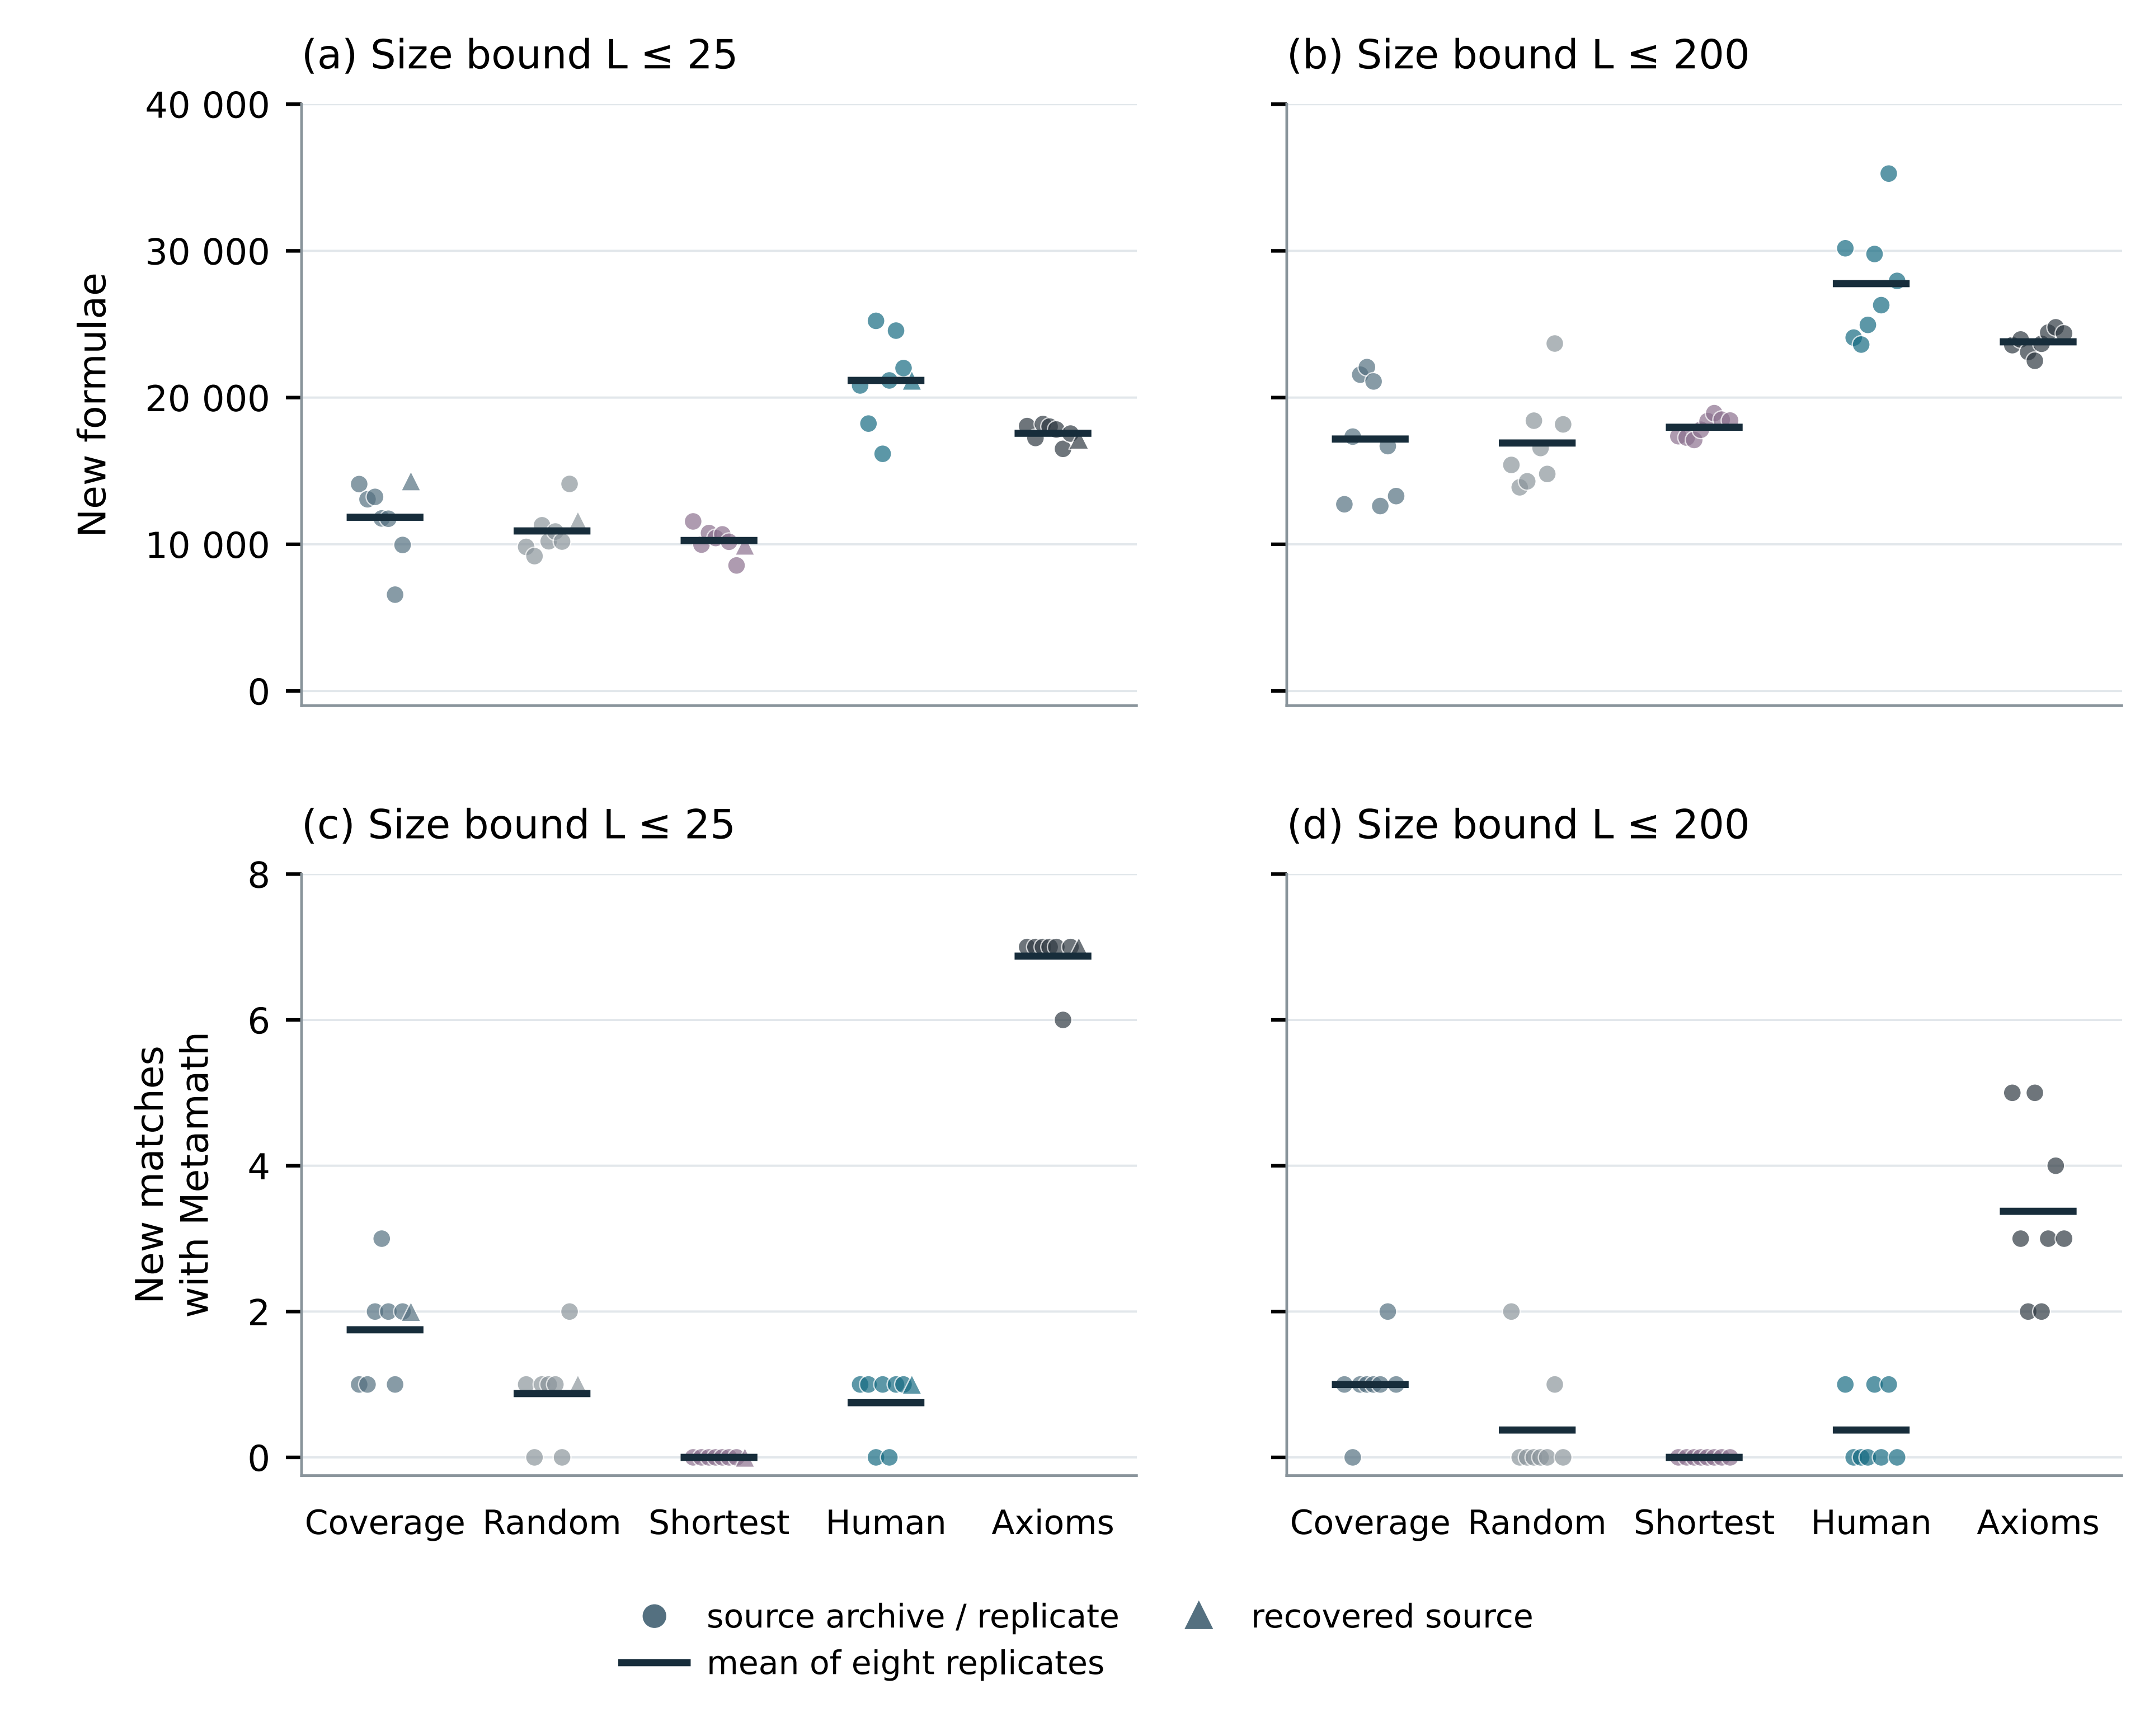
\includegraphics[width=\linewidth,height=.67\textheight,keepaspectratio]{Fig8.png}
\caption{Utility of the starting representation under direct continuation. Upper panels show new canonical formulae outside the common source archive; lower panels show new exact matches against 108 evaluation statements. Points mark eight common sources, line segments mark means, and triangles mark the recovery source. Axis labels denote coverage, random, shortest, and human anchors, then axioms. The first four variants use eight anchors and the last uses no additional anchors. The budget includes preparation and storage; human coverage supplies a secondary outcome}\label{fig:8}
\end{figure}

\subsubsection*{E.1.6. Support costs and scope of generalisation}\label{e.1.6.-support-costs-and-scope-of-generalisation}
\addcontentsline{toc}{subsubsection}{E.1.6. Support costs and scope of generalisation}

Eight anchors can require different amounts of memory. The human variant starts with a mean of 21.375 proof-support vertices at both bounds, versus 54.125 and 56.125 for the random variant; nevertheless, mean peak memory during human-anchor continuation reaches about 499 and 540 MB, versus 368 and 381 MB for random anchors. More compact starting support therefore does not guarantee lower memory use during subsequent growth.

Human anchor sets offer limited diversity. Across 16 sources, only three distinct sets occur, with frequencies 11, 3, and 2. Initial states reveal algorithmic sensitivity but cannot replace a sample of diverse mathematical theories, so the confirmed effect concerns these sources, this fixed generator, and this budget.

Continuation itself receives no targets, but external lemmas shape the human starting set. Its outcome therefore supplies no evidence for an internally emergent or scale-invariant topology. These experiments establish neither the degree distribution of the infinite space nor optimality of anchor selection.

\subsubsection*{E.1.7. Short test of the branch combination}\label{e.1.7.-short-test-of-the-branch-combination}
\addcontentsline{toc}{subsubsection}{E.1.7. Short test of the branch combination}

The short test reports mean new-formula counts at 20 CPU-seconds separately for development and transfer. Each cell averages two sources. Combining both groups into one confirmatory sample would erase their distinct roles (Table 18).

\begingroup
\small
\setlength{\tabcolsep}{3pt}
\renewcommand{\arraystretch}{1.13}

\begin{longtable}[]{@{}
  >{\raggedright\arraybackslash}p{(\linewidth - 8\tabcolsep) * \real{0.1824}}
  >{\raggedleft\arraybackslash}p{(\linewidth - 8\tabcolsep) * \real{0.2155}}
  >{\raggedleft\arraybackslash}p{(\linewidth - 8\tabcolsep) * \real{0.2267}}
  >{\raggedleft\arraybackslash}p{(\linewidth - 8\tabcolsep) * \real{0.1826}}
  >{\raggedleft\arraybackslash}p{(\linewidth - 8\tabcolsep) * \real{0.1928}}@{}}
\caption{Mean new-formula counts in the short context-transfer test, by source group and size bound}\label{tab:18}\tabularnewline
\toprule\noalign{}
\begin{minipage}[b]{\linewidth}\raggedright
\textbf{Condition}
\end{minipage} & \begin{minipage}[b]{\linewidth}\raggedleft
\textbf{Development, 25}
\end{minipage} & \begin{minipage}[b]{\linewidth}\raggedleft
\textbf{Development, 200}
\end{minipage} & \begin{minipage}[b]{\linewidth}\raggedleft
\textbf{Transfer, 25}
\end{minipage} & \begin{minipage}[b]{\linewidth}\raggedleft
\textbf{Transfer, 200}
\end{minipage} \\
\midrule\noalign{}
\endfirsthead
\toprule\noalign{}
\begin{minipage}[b]{\linewidth}\raggedright
\textbf{Condition}
\end{minipage} & \begin{minipage}[b]{\linewidth}\raggedleft
\textbf{Development, 25}
\end{minipage} & \begin{minipage}[b]{\linewidth}\raggedleft
\textbf{Development, 200}
\end{minipage} & \begin{minipage}[b]{\linewidth}\raggedleft
\textbf{Transfer, 25}
\end{minipage} & \begin{minipage}[b]{\linewidth}\raggedleft
\textbf{Transfer, 200}
\end{minipage} \\
\midrule\noalign{}
\endhead
\bottomrule\noalign{}
\endlastfoot
A & 26 190 & 38 504 & 28 073 & 38 202.5 \\
A+A & 17 075 & 22 570 & 17 247.5 & 23 374.5 \\
A+S & 26 860 & 33 578 & 26 918.5 & 32 658 \\
Probe & 26 735 & 33 782 & 27 031.5 & 32 869 \\
Random & 28 435 & 33 640 & 23 184 & 34 504 \\
Context & 29 325.5 & 40 347 & 28 695.5 & 41 501.5 \\
\end{longtable}

\endgroup

On the four transfer sources, the Context/A ratio of means exceeds one by 2.2\% at \(L = 25\) and 8.6\% at \(L = 200\). The advantage does not hold trajectory by trajectory: Context loses to the axiom-only control on one of two sources in each stratum. Across eight short source blocks, Context outperforms A in five blocks, A+A in eight, both A+S and Probe in six, and random replacement in seven. These frequencies describe the panel and do not replace a statistical test.

Checks confirm that the three probe conditions share starting anchors, donor proposals, and the exchange-witness catalogue within each short block. Different probe sets therefore cannot explain the contrast. Scoring and constructing the new basis consume CPU time, and soft phase boundaries leave timing effects. Both short groups pass the pre-specified rule for proceeding to the long test, and independent replay covers 1 927 checkpoint certificates. The longer series tests whether this short-budget advantage persists.

\subsubsection*{E.1.8. Long test of context transfer}\label{e.1.8.-long-test-of-context-transfer}
\addcontentsline{toc}{subsubsection}{E.1.8. Long test of context transfer}

The long test reports mean outcomes on four new sources at the larger budgets. The table retains all six conditions. No reruns replace outcomes that lose to the control (Table 19).

\begingroup
\small
\setlength{\tabcolsep}{3pt}
\renewcommand{\arraystretch}{1.13}

\begin{longtable}[]{@{}
  >{\raggedright\arraybackslash}p{(\linewidth - 8\tabcolsep) * \real{0.2000}}
  >{\raggedleft\arraybackslash}p{(\linewidth - 8\tabcolsep) * \real{0.2000}}
  >{\raggedleft\arraybackslash}p{(\linewidth - 8\tabcolsep) * \real{0.2000}}
  >{\raggedleft\arraybackslash}p{(\linewidth - 8\tabcolsep) * \real{0.2000}}
  >{\raggedleft\arraybackslash}p{(\linewidth - 8\tabcolsep) * \real{0.2000}}@{}}
\caption{Mean new-formula counts in the long context-transfer test, by budget and size bound}\label{tab:19}\tabularnewline
\toprule\noalign{}
\begin{minipage}[b]{\linewidth}\raggedright
\textbf{Condition}
\end{minipage} & \begin{minipage}[b]{\linewidth}\raggedleft
\textbf{60 s, 25}
\end{minipage} & \begin{minipage}[b]{\linewidth}\raggedleft
\textbf{60 s, 200}
\end{minipage} & \begin{minipage}[b]{\linewidth}\raggedleft
\textbf{180 s, 25}
\end{minipage} & \begin{minipage}[b]{\linewidth}\raggedleft
\textbf{180 s, 200}
\end{minipage} \\
\midrule\noalign{}
\endfirsthead
\toprule\noalign{}
\begin{minipage}[b]{\linewidth}\raggedright
\textbf{Condition}
\end{minipage} & \begin{minipage}[b]{\linewidth}\raggedleft
\textbf{60 s, 25}
\end{minipage} & \begin{minipage}[b]{\linewidth}\raggedleft
\textbf{60 s, 200}
\end{minipage} & \begin{minipage}[b]{\linewidth}\raggedleft
\textbf{180 s, 25}
\end{minipage} & \begin{minipage}[b]{\linewidth}\raggedleft
\textbf{180 s, 200}
\end{minipage} \\
\midrule\noalign{}
\endhead
\bottomrule\noalign{}
\endlastfoot
A & 65 743 & 94 744.5 & 156 632 & 223 483 \\
A+A & 38 939.5 & 54 681.5 & 98 868.5 & 143 355 \\
A+S & 60 052 & 75 167.5 & 129 953.5 & 178 756 \\
Probe & 60 324.5 & 75 376.5 & 129 737 & 178 982 \\
Random & 49 550.5 & 72 067 & 115 168 & 188 893 \\
Context & 63 000.5 & 78 985.5 & 133 480.5 & 203 247 \\
\end{longtable}

\endgroup

At 60 CPU-seconds, the Context/A ratio of means falls below one by 4.2\% at \(L = 25\) and 16.6\% at \(L = 200\); at 180 CPU-seconds, the deficits reach 14.8\% and 9.1\%. The overall criterion from the protocol fails at both budgets. Proof trajectories still complete correctly, but these results do not confirm a consistent advantage for this combination.

Context-based selection nevertheless differs from random transfer. It outperforms random replacement in each of the four long blocks at each budget; against A+S it wins in three of four blocks at 60 seconds and two at 180, against Probe it wins in two of four at each budget, and against the axiom-only control it wins in only one of four at each budget. Utility of context-based choice within the two-branch architecture therefore does not imply that the architecture itself repays the budget split (Fig. 9).

\begin{figure}[!htbp]
\centering
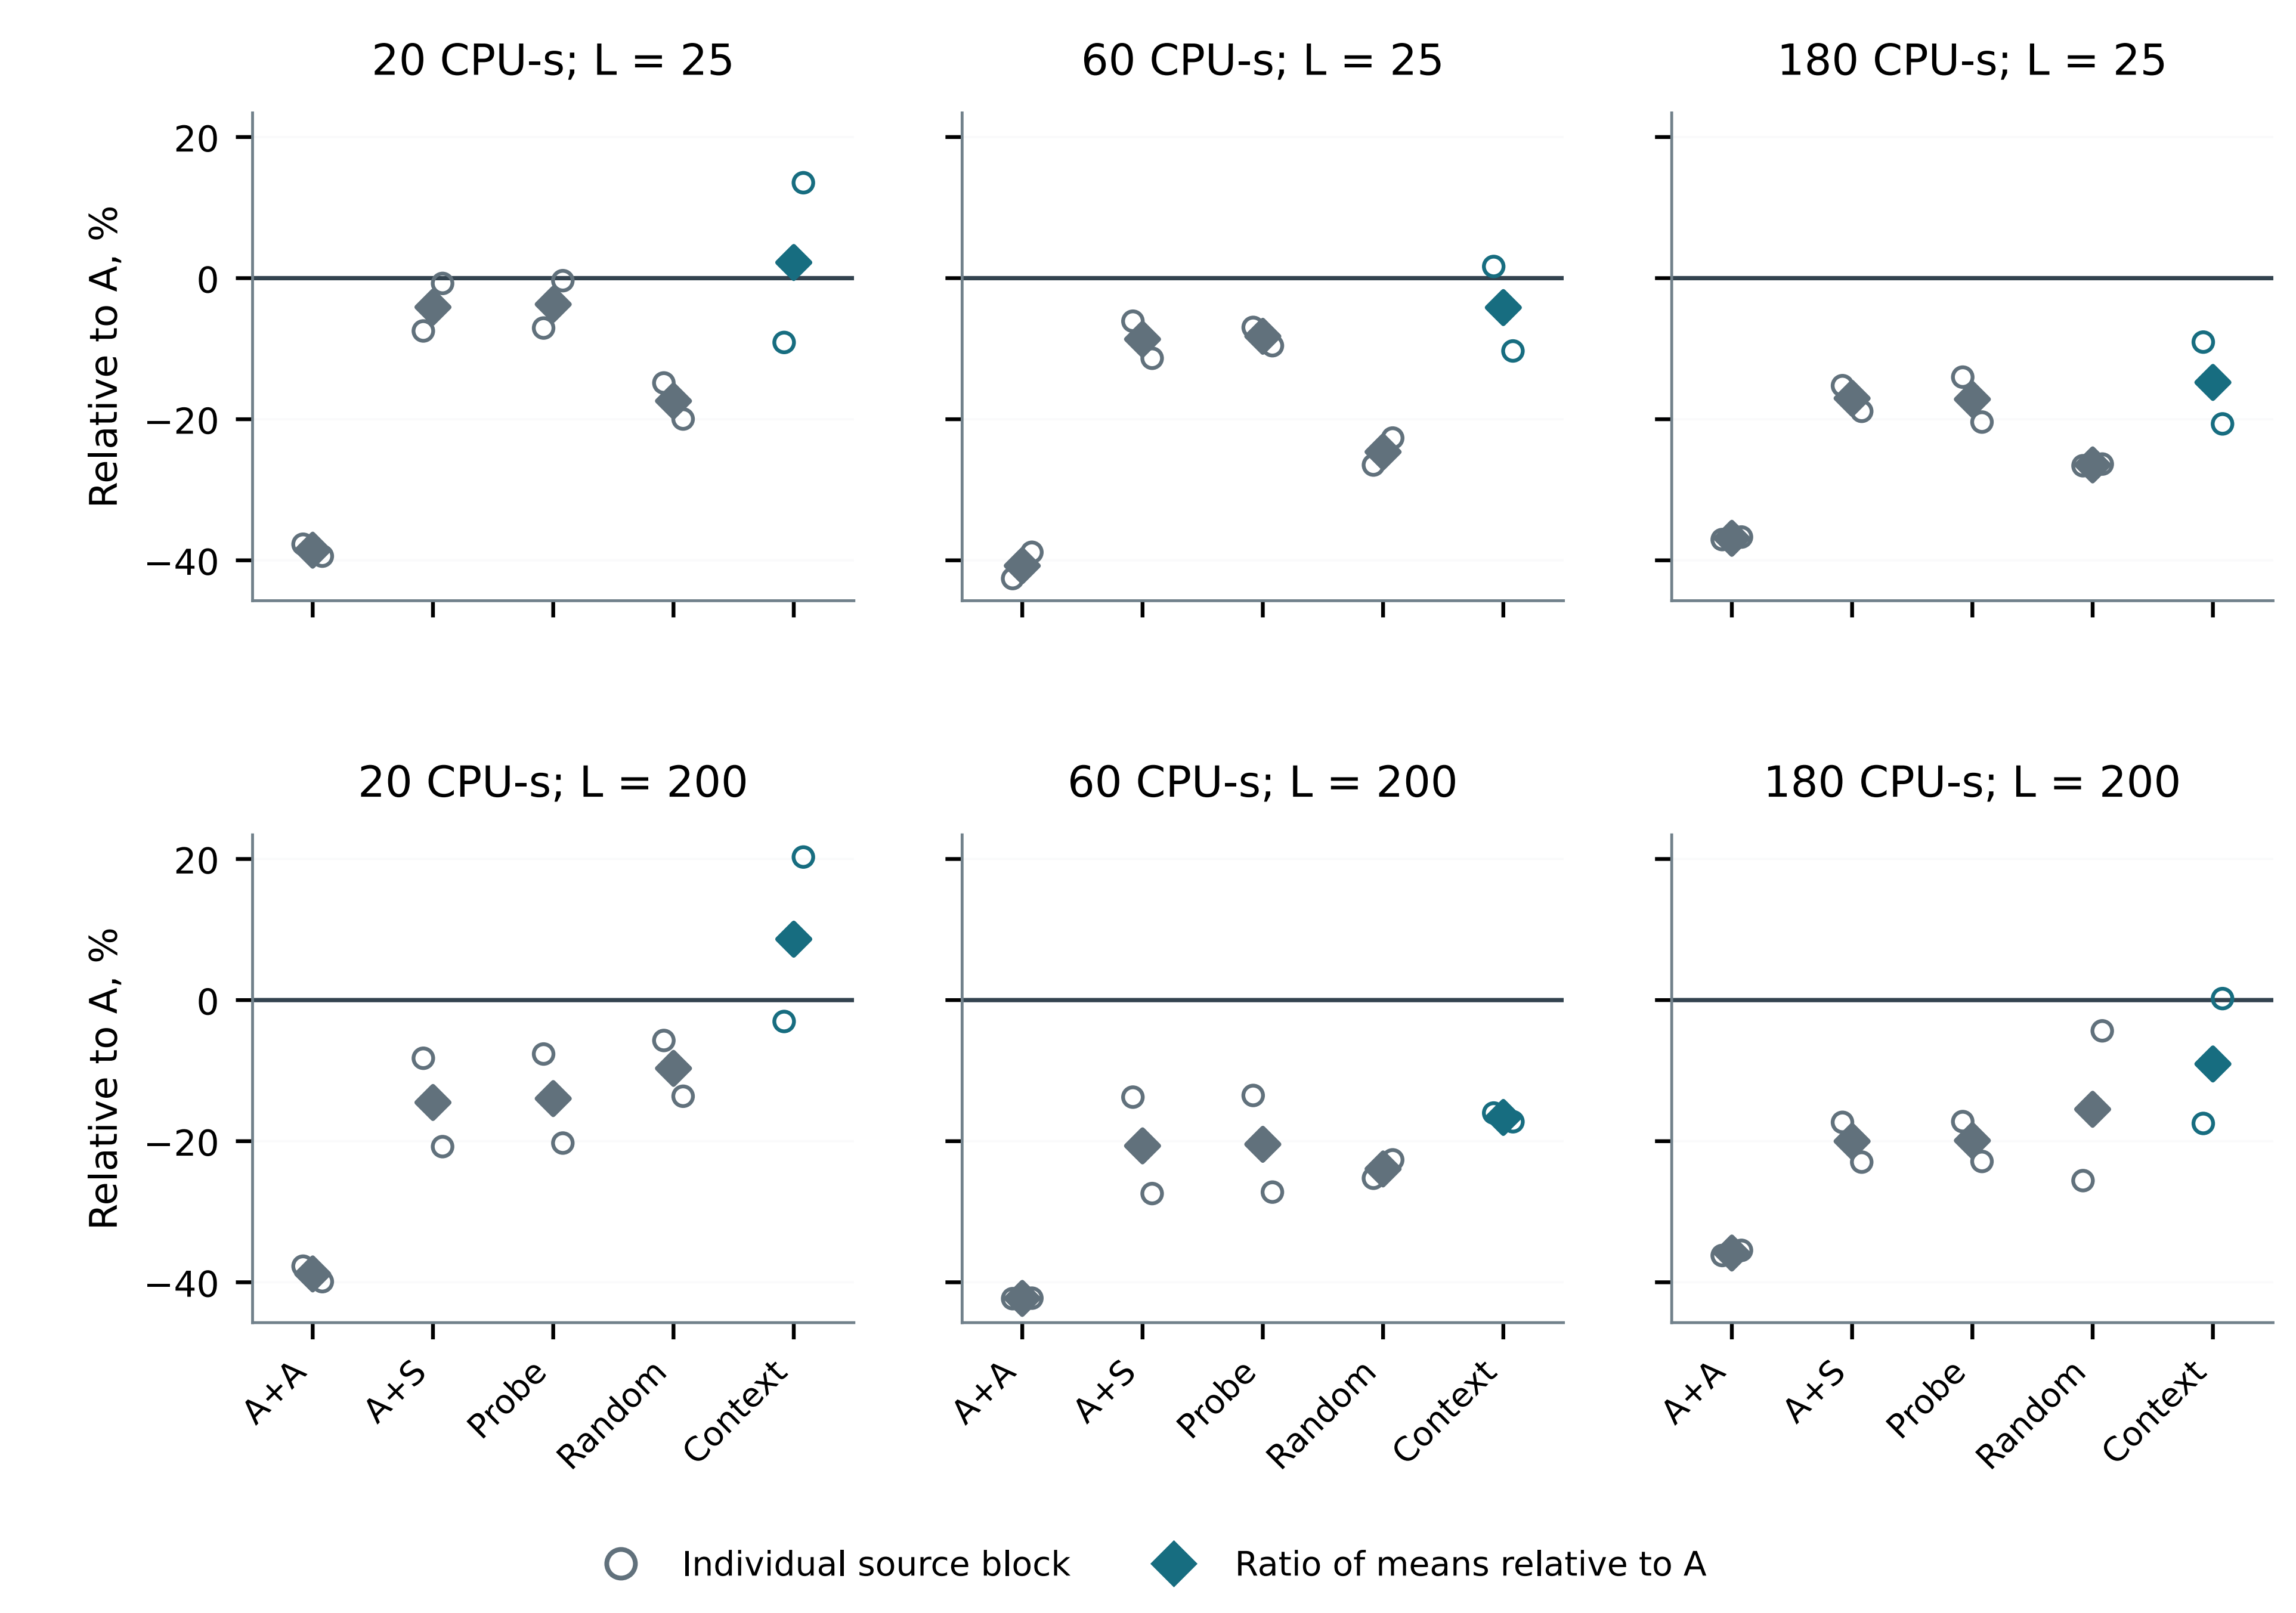
\includegraphics[width=\linewidth,height=.67\textheight,keepaspectratio]{Fig9.png}
\caption{Context transfer and controls relative to single axiomatic growth. Circles mark individual source blocks, and diamonds mark the ratio of means to the axiom-only control minus one; the plot omits significance intervals. Each panel contains two blocks. The 20-second group uses different sources from the 60- and 180-second groups, so no lines imply a causal budget effect across groups}\label{fig:9}
\end{figure}

All 44 branch stages in the 60-second series stop at the CPU boundary. At 180 seconds, 40 stages stop for the same reason and four cross the final boundary while storing a complete layer; those four final storage commits contain 12 662 additional formulae in total and receive no credit. No generation, vertex, or memory safeguard determines a stop in the records, and peak memory reaches 0.68--1.48 GiB at 60 seconds and 1.65--3.41 GiB at 180, so these data do not establish saturation of the proof space.

The long series passes checks on 4 052 checkpoint certificates, giving 5 979 together with the short groups. At 60 seconds, full-prefix storage consumes a mean of 9.39 CPU-seconds for A and 14.96 for Context. This profile describes costs rather than establishing a cause of the loss; subtracting storage time for only one method would distort the comparison, whereas a common storage change would require a new comparison of all conditions.

Starting bases coincide across conditions within every block. Exchange catalogues match literally in six of eight long source--budget combinations and differ in local conclusion identifiers in two; a separate formula-level check confirms identical proposals and witnesses for all three probe conditions in all eight combinations. This agreement does not imply identical donor trajectories or costs, because CPU time determines stopping and donor-archive sizes can differ.

\subsubsection*{E.1.9. Human coverage of combined trajectories}\label{e.1.9.-human-coverage-of-combined-trajectories}
\addcontentsline{toc}{subsubsection}{E.1.9. Human coverage of combined trajectories}

After all series finished, a separate analysis counted exact matches to the same 108 Metamath evaluation statements for 96 final archives that qualified for credit. It compares canonical formulae, excludes source matches from gains, and supplies none of the statements to the generator as a target. The table averages new exact matches over two sources per stratum and reports the transfer group, not the development group, at 20 seconds (Table 20).

\begingroup
\small
\setlength{\tabcolsep}{3pt}
\renewcommand{\arraystretch}{1.13}

\begin{longtable}[]{@{}
  >{\raggedright\arraybackslash}p{(\linewidth - 12\tabcolsep) * \real{0.1429}}
  >{\raggedleft\arraybackslash}p{(\linewidth - 12\tabcolsep) * \real{0.1429}}
  >{\raggedleft\arraybackslash}p{(\linewidth - 12\tabcolsep) * \real{0.1429}}
  >{\raggedleft\arraybackslash}p{(\linewidth - 12\tabcolsep) * \real{0.1429}}
  >{\raggedleft\arraybackslash}p{(\linewidth - 12\tabcolsep) * \real{0.1429}}
  >{\raggedleft\arraybackslash}p{(\linewidth - 12\tabcolsep) * \real{0.1429}}
  >{\raggedleft\arraybackslash}p{(\linewidth - 12\tabcolsep) * \real{0.1429}}@{}}
\caption{New exact human-reference matches in the context-transfer series}\label{tab:20}\tabularnewline
\toprule\noalign{}
\begin{minipage}[b]{\linewidth}\raggedright
\textbf{Condition}
\end{minipage} & \begin{minipage}[b]{\linewidth}\raggedleft
\textbf{20 s,} \(L = 25\)
\end{minipage} & \begin{minipage}[b]{\linewidth}\raggedleft
\textbf{20 s,} \(L = 200\)
\end{minipage} & \begin{minipage}[b]{\linewidth}\raggedleft
\textbf{60 s,} \(L = 25\)
\end{minipage} & \begin{minipage}[b]{\linewidth}\raggedleft
\textbf{60 s,} \(L = 200\)
\end{minipage} & \begin{minipage}[b]{\linewidth}\raggedleft
\textbf{180 s,} \(L = 25\)
\end{minipage} & \begin{minipage}[b]{\linewidth}\raggedleft
\textbf{180 s,} \(L = 200\)
\end{minipage} \\
\midrule\noalign{}
\endfirsthead
\toprule\noalign{}
\begin{minipage}[b]{\linewidth}\raggedright
\textbf{Condition}
\end{minipage} & \begin{minipage}[b]{\linewidth}\raggedleft
\textbf{20 s,} \(L = 25\)
\end{minipage} & \begin{minipage}[b]{\linewidth}\raggedleft
\textbf{20 s,} \(L = 200\)
\end{minipage} & \begin{minipage}[b]{\linewidth}\raggedleft
\textbf{60 s,} \(L = 25\)
\end{minipage} & \begin{minipage}[b]{\linewidth}\raggedleft
\textbf{60 s,} \(L = 200\)
\end{minipage} & \begin{minipage}[b]{\linewidth}\raggedleft
\textbf{180 s,} \(L = 25\)
\end{minipage} & \begin{minipage}[b]{\linewidth}\raggedleft
\textbf{180 s,} \(L = 200\)
\end{minipage} \\
\midrule\noalign{}
\endhead
\bottomrule\noalign{}
\endlastfoot
A & 7 & 5 & 6.5 & 5.5 & 6.5 & 5.5 \\
A+A & 7 & 2 & 6.5 & 5.5 & 6.5 & 5.5 \\
A+S & 7 & 2 & 6.5 & 5.5 & 6.5 & 5.5 \\
Probe & 7 & 2 & 6.5 & 5.5 & 6.5 & 5.5 \\
Random & 7 & 2 & 6.5 & 6 & 6.5 & 6 \\
Context & 7 & 2 & 6.5 & 5.5 & 6.5 & 5.5 \\
\end{longtable}

\endgroup

This post hoc diagnosis adds neither a new primary metric nor a change to the selection rule. In the long groups, Context and A yield identical gains in every source block, whereas at \(L = 200\) random exchange reaches one more human statement on one source despite generating fewer new schemata; table values do not change from 60 to 180 seconds even though formula counts rise substantially. On these data, a larger syntactic archive therefore does not imply broader coverage of this human fragment.

The development group yields seven new matches for every condition at \(L = 25\); at \(L = 200\), A averages six, random exchange 3.5, and the other conditions three. Context never exceeds A on this measure in any of the four groups, and a complete separate report retains source, new, and absent statement lists for every trajectory. We check the entire archive that qualifies for credit, not only its final active set, and do not recount substitution matches. Reusing this public set supplies no independent mathematical sample.

\section*{Appendix F. Reproducibility and audit}\label{appendix-f.-reproducibility-and-audit}
\addcontentsline{toc}{section}{Appendix F. Reproducibility and audit}

\subsection*{F.1. Reproducibility and data provenance}\label{f.1.-reproducibility-and-data-provenance}
\addcontentsline{toc}{subsection}{F.1. Reproducibility and data provenance}

\subsubsection*{F.1.1. Frozen series}\label{f.1.1.-frozen-series}
\addcontentsline{toc}{subsubsection}{F.1.1. Frozen series}

The original series \path{skeleton-opportunities-20261006-v1} uses a manifest with SHA-256 \path{0e7a29a689803dcf3ffff23bff1d1f78352dffa1f2f3b30875581c7dce69f380}. Cluster reports \path{screen_gate/result.json} and \path{final_audit/result.json} contain full replay of 336 screening and 124 admissible confirmation trajectories. The second report retains its incomplete status.

The recovery series \path{skeleton-opportunities-repair-20261006-v2} uses a manifest with SHA-256 \path{90fb90960078280acfa3f4c57eb90be66eefaec75223c3eefe426cdcbb9cb344}. A separate file, \path{output/article1_recovery_analysis_20261006/result.json}, holds the combined result; independent replay covers the four new conditions, whereas checks of linked reports and checksums cover the 124 earlier trajectories. The final decision under the frozen protocol remains conditional, and the original results remain intact.

The direct-continuation series \path{skeleton-utility-final-20261006-v1} uses a manifest with SHA-256 \path{50b4b1353987c7f6729aeefc9c337148470a8b5feb0cca1e8139e9a55d5a1400}. Its \path{download/results/final_audit/result.json} records 80 conditions, 16 blocks, and successful full independent replay. The whole-series audit separately required 4 057.66 CPU-seconds, outside the 30-second continuation budgets.

These three series ran on a high-performance computing cluster, with one CPU per condition and Python 3.11.4. The frozen packages include executable versions, parameters, initial states, condition order, and source certificates. Peak memory measures the process rather than the resource request to the scheduler.

\subsubsection*{F.1.2. Context transfer and larger budgets}\label{f.1.2.-context-transfer-and-larger-budgets}
\addcontentsline{toc}{subsubsection}{F.1.2. Context transfer and larger budgets}

The context-transfer development series uses a manifest with SHA-256 \path{b52564937a1a0bd9a587b1444baa4062df80d4a8e6db94ccf5312dc53af3a8eb}, and the short transfer series uses \path{c25b305201eee0df5c119fed9025c19f59858de92764508ecbfec1e71ca626aa}. Each contains 24 conditions, its own full audit, and a separate descriptive report; the independent checker replays each new proof once, then compares records from its earlier checks byte for byte in all later prefixes. Sources correspond to construction states 1301--1302 and 1303--1304 at each size bound, and auditing both short groups required a further 236.41 CPU-seconds beyond continuation budgets.

The long series uses source states 1305--1306. Its manifest SHA-256 values for 60 and 180 CPU-seconds respectively read \path{421052bf637e160cc7c2a0d5757b7f7c3b00cde5dffec5afabb5908a58b18154} and \path{4602b2cd099087b41ee75b5da4b50c9a3328a70ef0b254a193f373d12f0daea6}. Generator, selector, and independent-checker code match byte for byte across all four packages, whereas the protocols explicitly retain differences such as the long runs' higher safeguards. The new groups run locally with Python 3.13.3 and measure CPU time separately in each worker process, excluding the outer wrapper and later audit from the algorithmic budget; their absolute-speed estimates remain separate from the cluster experiments.

Independent audits of the two long groups required 1 056.40 CPU-seconds in total. They checked 4 052 checkpoints and every exchange witness and retained both negative decisions on overall superiority; the separate report \path{portfolio_human_exact.json} links the human comparison to hashes of 96 final certificates that qualified for credit and to the unchanged evaluation set. Repeating formula comparisons does not constitute another independent proof replay.

The data register and editorial manifest link complete paths, execution receipts, and checksums. Twenty-one unit and integration tests check the short protocol, and the first development run partly overlapped those tests in time, whereas the transfer and long groups did not share that overlap. These tests do not replace replay of the experimental certificates.

\subsubsection*{F.1.3. Continuous mechanism and fragment library}\label{f.1.3.-continuous-mechanism-and-fragment-library}
\addcontentsline{toc}{subsubsection}{F.1.3. Continuous mechanism and fragment library}

The short series \path{article1_fragments_pilot_20261007_v1} uses a manifest with SHA-256 \path{4b63c866967d04349130e25b3e0b62b5b4d3c9b960514bafc094804470e4ac37}. Its main and supplementary checks cover 18 trajectories and 819 checkpoints and count 462 562 records across trajectories, so the last count does not measure the cardinality of the union of distinct theorems. The short test motivates the additional passive-library condition, not revision of existing results.

The expanded series \path{article1_fragments_long_20261007_v1} uses a manifest with SHA-256 \path{8094aa706d0b3883514d1fc9263057fd470dd10d1d6ca5d7239df5a5cc62e410} and protocol SHA-256 \path{7f9dc5a6c9fefff47df096389d396e86f31fda5105ecf23cfe5fdfcf7b876460}. Its four scheduling states carry numbers 7201--7204 and do not repeat the short series' 7101--7102; analysis uses the last receipt that the process finished writing before each budget boundary and retains terminal stopping reasons and late records without credit. Every outcome links to a frozen configuration, and no rerun replaces a result.

The calculation ran locally with Python 3.13.3 and two concurrent search processes. An independent checker replayed complete trajectories in separate processes and could overlap conditions that still ran; the budget measures each search process's CPU time, but shared hardware load can still affect operation speed. Small timing differences therefore imply no isolated hardware acceleration, and absolute speeds from this group remain separate from cluster measurements.

The file \path{fragments_summary.json} contains all 48 outcomes, nested time checkpoints, paired differences, stopping reasons, costs, and checks of common complete prefixes for O and OB. For propositional conditions it also retains exact source, new, absent, active, and library matches to the earlier 108 evaluation statements, and the editorial manifest links this analysis to the combined independent audit and individual result hashes. The analysis runs no search, changes no primary measure, and creates no independent human sample.

\subsubsection*{F.1.4. Checks of downloaded results and the benchmark}\label{f.1.4.-checks-of-downloaded-results-and-the-benchmark}
\addcontentsline{toc}{subsubsection}{F.1.4. Checks of downloaded results and the benchmark}

The local report \path{output/article1_utility_verification_20261006/result.json} checks receipts for 80 trajectories and checksums for 2 014 checkpoint certificates. It recalculates novelty relative to the common archive and exact human matches and reproduces aggregate analysis; six floating-point log fields differ from the cluster calculation by no more than \(1.78 \cdot 10^{- 15}\), whereas integer counts and decisions match. This local check covers data and aggregation rather than a second full replay of all elementary proofs; the cluster auditor checked human substitution matches, but the local check did not recalculate them.

The \path{set.mm} version uses commit \path{584b6852f57f281e9be1793332f1e52e077693c8} and source-file SHA-256 \path{90de6bac87d549023fc83fb698a1baacfed3f99b71438722171674f16777c881}. The experiment package contains the resulting sets and their extraction rules. No evaluation formula enters the generator as a target.

\subsubsection*{F.1.5. Additional sources and audit limits}\label{f.1.5.-additional-sources-and-audit-limits}
\addcontentsline{toc}{subsubsection}{F.1.5. Additional sources and audit limits}

The main generator resides in \path{src/hilbert/schema_generator.py}. The certificate pipeline, independent checker, frozen protocols, and aggregation reside in \path{hpc/article1_skeleton/}. To reproduce the figures, use the versions in the relevant packages; current working files may differ.

H14 generational sizes come from \path{results/article1/ex0/d3_confirmatory_v2/w4_requested_rep1/results_d3.json}. Pruning losses on the exact registry link to \path{results/article1/revision_2026-09-07/pruning_oracle.json}, and the KSP resource bound links to \path{results/article1/completion_2026-09-17/resource_transfer_checks.json}. For the identity lower bound, independent checking covers 1 901 166 formulae and 1 901 165 MP applications; finite tests of the Catalan family check sizes, injectivity, and inference steps. These tests supplement the mathematical proof rather than replacing formalisation in a proof assistant.

The editorial package links text, figures, tables, and source reports through checksums. Its claim--evidence matrix and availability statement distinguish complete checks from future tasks.

\section*{Appendix G. Additional checks}\label{appendix-g.-additional-checks}
\addcontentsline{toc}{section}{Appendix G. Additional checks}

\subsection*{G.1. Resource cost of a ready-made identity}\label{g.1.-resource-cost-of-a-ready-made-identity}
\addcontentsline{toc}{subsection}{G.1. Resource cost of a ready-made identity}

The identity calculation uses \(J = X \rightarrow X\), \(P = X \rightarrow (J \rightarrow X)\), and \(Q = X \rightarrow (X \rightarrow X)\). The following proof derives the identity through two applications of modus ponens. Its explicit intermediate formulae provide the resource accounting below:

\[\fitdisplay{\begin{matrix}
1. & P & K, \\
2. & P \rightarrow (Q \rightarrow J) & S, \\
3. & Q \rightarrow J & MP(1,2), \\
4. & Q & K, \\
5. & J & MP(4,3).
\end{matrix}}\]

This calculation uses only the leaf metric \(\ell_{leaf}\). If \(X\) contains \(n\) variable occurrences, the sizes of the five formulae equal \(4n\), \(9n\), \(5n\), \(3n\), and \(2n\), and the proof reaches height two when axioms start at height zero. Using \(X \rightarrow X\) within a window of size \(m\) requires \(n \leq \lfloor m/2\rfloor\), so expansion fits within

\[\fitdisplay{\kappa(m) = max\{ m,9\lfloor m/2\rfloor\}.}\]

The complete closure through eight leaves passes checking but contains no \(p \rightarrow p\), whereas the proof above fits within nine leaves. The lower bound therefore follows from a finite computational check of this particular calculus, not merely from the upper-bound construction; the linked report retains checksums and independent checking of the smaller window. The factor \(9/2\) does not automatically transfer to other axiomatisations, search time, or certificate length.

\subsection*{G.2. Role of the exact finite benchmark}\label{g.2.-role-of-the-exact-finite-benchmark}
\addcontentsline{toc}{subsection}{G.2. Role of the exact finite benchmark}

The space \(U_{m}\) contains all canonical implicational formulae with at most \(m\) variable occurrences. Its deductive closure \(C_{m} \subseteq U_{m}\) contains only formulae whose derivation keeps every intermediate formula within that space. With a finite complete rule registry, saturation therefore computes the exact least fixed point.

We use the benchmark to measure coverage, find lost lemmas, and check whether search recovers after pruning. It does not replace the main method. In the atlas, the largest window contains 11 993 273 546 admissible formulae, and its closure contains 188 904 984 formulae, including 612 617 that do not instantiate axioms. These counts explain why coverage needs a separate measure on the non-axiomatic increment.

Two independent implementations agree on rank sets and axiom sets for \(U_{3},\ldots,U_{8}\). The C implementation that passed these smaller-window checks fully enumerates the larger windows \(U_{9},\ldots,U_{11}\), but this does not supply independent full certification of the larger spaces. Exactness of a finite benchmark does not imply completeness for unbounded logic.

\subsection*{G.3. Preliminary checks and negative results}\label{g.3.-preliminary-checks-and-negative-results}
\addcontentsline{toc}{subsection}{G.3. Preliminary checks and negative results}

The following experiments precede the main text's series with certificates. They use different budgets and partly target-dependent criteria, and the old epoch interface does not carry end-to-end certificates. They expose component limitations rather than adding an independent sample to the primary statistical comparisons (Fig. 10).

\begin{figure}[!htbp]
\centering
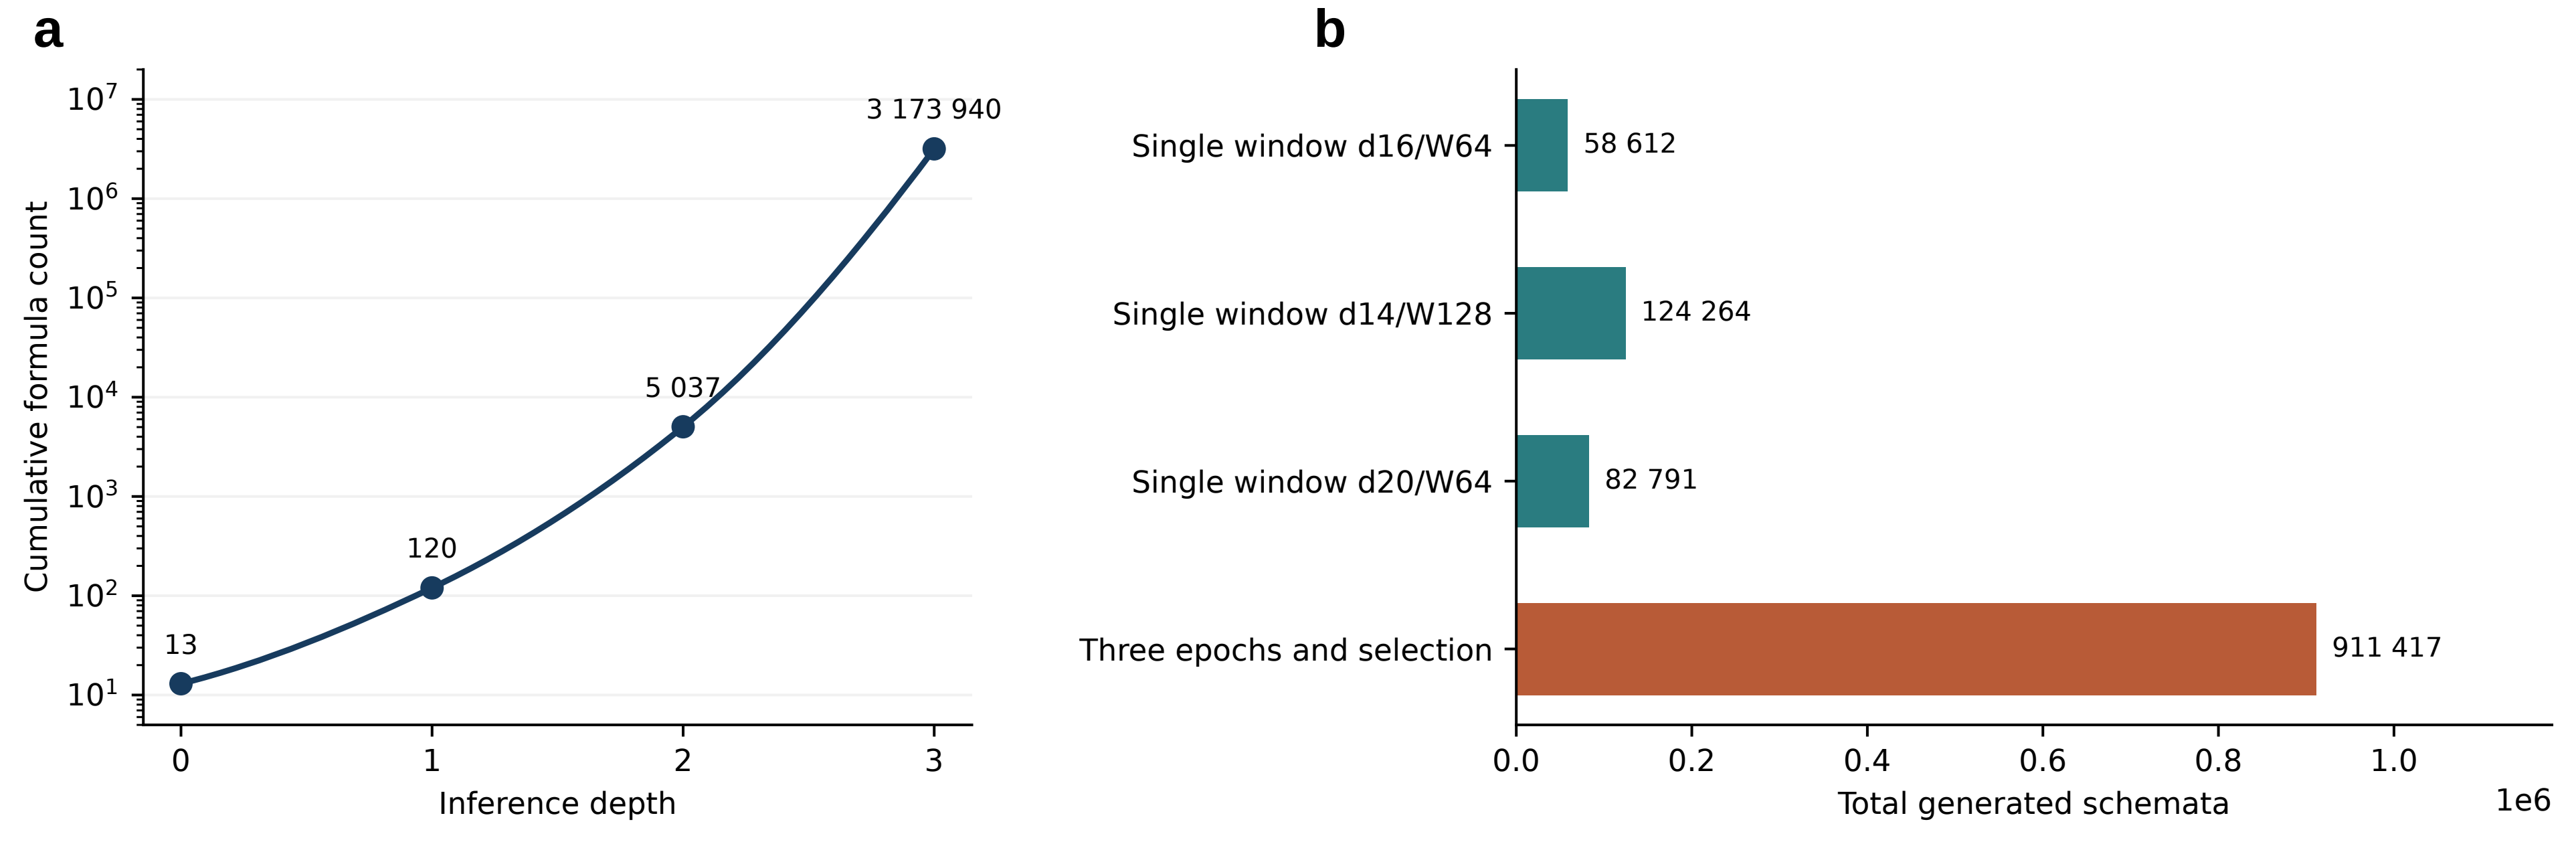
\includegraphics[width=\linewidth,height=.67\textheight,keepaspectratio]{Fig10.png}
\caption{Preliminary data: H14 growth and the cost of the old epoch-based selection. The left panel marks every measured depth and joins them with a monotone cubic spline in log count, solely as a visual guide. Every variant on the right reaches 11 of 14 control statements that the procedure knows in advance. Cycle costs include measurement runs; the panels concern different configurations and do not form a common scaling curve}\label{fig:10}
\end{figure}

\subsubsection*{G.3.1. Target-free selection}\label{g.3.1.-target-free-selection}
\addcontentsline{toc}{subsubsection}{G.3.1. Target-free selection}

The fixed regime of depth 8 and width 64 compares arrival order, an internal score for repeated derivations and size, and a target-aware ranker. Target-free variants use the control list only to record outcomes, assign zero target weights, and never adapt width to hits. Their selection therefore receives no target signal from that list (Table 21).

\begingroup
\small
\setlength{\tabcolsep}{3pt}
\renewcommand{\arraystretch}{1.13}

\begin{longtable}[]{@{}
  >{\raggedright\arraybackslash}p{(\linewidth - 4\tabcolsep) * \real{0.4344}}
  >{\raggedleft\arraybackslash}p{(\linewidth - 4\tabcolsep) * \real{0.3261}}
  >{\raggedleft\arraybackslash}p{(\linewidth - 4\tabcolsep) * \real{0.2395}}@{}}
\caption{Control-statement coverage and formula counts under preliminary target-free selection}\label{tab:21}\tabularnewline
\toprule\noalign{}
\begin{minipage}[b]{\linewidth}\raggedright
\textbf{Logical system and policy}
\end{minipage} & \begin{minipage}[b]{\linewidth}\raggedleft
\textbf{Control statements}
\end{minipage} & \begin{minipage}[b]{\linewidth}\raggedleft
\textbf{Formulae}
\end{minipage} \\
\midrule\noalign{}
\endfirsthead
\toprule\noalign{}
\begin{minipage}[b]{\linewidth}\raggedright
\textbf{Logical system and policy}
\end{minipage} & \begin{minipage}[b]{\linewidth}\raggedleft
\textbf{Control statements}
\end{minipage} & \begin{minipage}[b]{\linewidth}\raggedleft
\textbf{Formulae}
\end{minipage} \\
\midrule\noalign{}
\endhead
\bottomrule\noalign{}
\endlastfoot
Prop., arrival order & 5/14 & 15 271 \\
Prop., internal utility & 6/14 & 14 301 \\
Prop., target-aware ranker & 10/14 & 13 126 \\
Modal, arrival order & 3/4 & 9 190 \\
Modal, internal utility & 4/4 & 11 520 \\
Modal, target-aware ranker & 4/4 & 10 809 \\
\end{longtable}

\endgroup

Internal signals change outcomes relative to queue order in these particular runs. Small control lists that the study knows in advance and one deterministic run per condition do not establish transfer to new theorem families. Equal outcomes for target-aware and target-free variants on four modal formulae may also reflect this set's ceiling.

\subsubsection*{G.3.2. Pruning and checks against the exact benchmark}\label{g.3.2.-pruning-and-checks-against-the-exact-benchmark}
\addcontentsline{toc}{subsubsection}{G.3.2. Pruning and checks against the exact benchmark}

In the production target-aware experiment at a common depth of 40, pruning removed 541 973 candidates from the passive pool while retaining materialised vertices. The vertex count reached 741 356, versus 676 062 without pruning. This observation concerns redistribution of the active budget in one target-aware regime; equal depth does not guarantee equal time, memory, or total cost, and it does not guarantee preservation of the entire space.

A stricter loss check uses an application registry that an earlier calculation produced in the exact KSP and KSP+I closures at nine leaves. It runs 36 variants across two systems, two queue orders, three attempt budgets, and three age thresholds. The experiment excludes candidate-birth costs and consequently evaluates scheduling, not the generator's total performance (Table 22).

\begingroup
\small
\setlength{\tabcolsep}{3pt}
\renewcommand{\arraystretch}{1.13}

\begin{longtable}[]{@{}
  >{\raggedright\arraybackslash}p{(\linewidth - 6\tabcolsep) * \real{0.3301}}
  >{\raggedleft\arraybackslash}p{(\linewidth - 6\tabcolsep) * \real{0.2233}}
  >{\raggedleft\arraybackslash}p{(\linewidth - 6\tabcolsep) * \real{0.2233}}
  >{\raggedleft\arraybackslash}p{(\linewidth - 6\tabcolsep) * \real{0.2233}}@{}}
\caption{Non-axiomatic coverage under age pruning on the exact KSP and KSP+I benchmarks}\label{tab:22}\tabularnewline
\toprule\noalign{}
\begin{minipage}[b]{\linewidth}\raggedright
\textbf{System and queue}
\end{minipage} & \begin{minipage}[b]{\linewidth}\raggedleft
\textbf{No pruning}
\end{minipage} & \begin{minipage}[b]{\linewidth}\raggedleft
\textbf{Age 8}
\end{minipage} & \begin{minipage}[b]{\linewidth}\raggedleft
\textbf{Age 64}
\end{minipage} \\
\midrule\noalign{}
\endfirsthead
\toprule\noalign{}
\begin{minipage}[b]{\linewidth}\raggedright
\textbf{System and queue}
\end{minipage} & \begin{minipage}[b]{\linewidth}\raggedleft
\textbf{No pruning}
\end{minipage} & \begin{minipage}[b]{\linewidth}\raggedleft
\textbf{Age 8}
\end{minipage} & \begin{minipage}[b]{\linewidth}\raggedleft
\textbf{Age 64}
\end{minipage} \\
\midrule\noalign{}
\endhead
\bottomrule\noalign{}
\endlastfoot
KSP, arrival order & 3 408 & 147 & 3 277 \\
KSP, utility & 3 408 & 148 & 3 277 \\
KSP+I, arrival order & 3 402 & 3 278 & 3 278 \\
KSP+I, utility & 3 402 & 3 278 & 3 278 \\
\end{longtable}

\endgroup

The table counts new non-axiomatic formulae under the full permitted budget, with age in scheduler attempts rather than production-generator generations. For KSP, threshold 8 retains 4.31\% of the derived part under arrival order and threshold 64 retains 96.16\%; at one quarter of the budget, utility yields 950 new formulae against 994 for arrival order, with corresponding KSP+I counts of 1 012 and 1 017. The simple score under test therefore shows no coverage advantage in these regimes (Fig. 11).

\begin{figure}[!htbp]
\centering
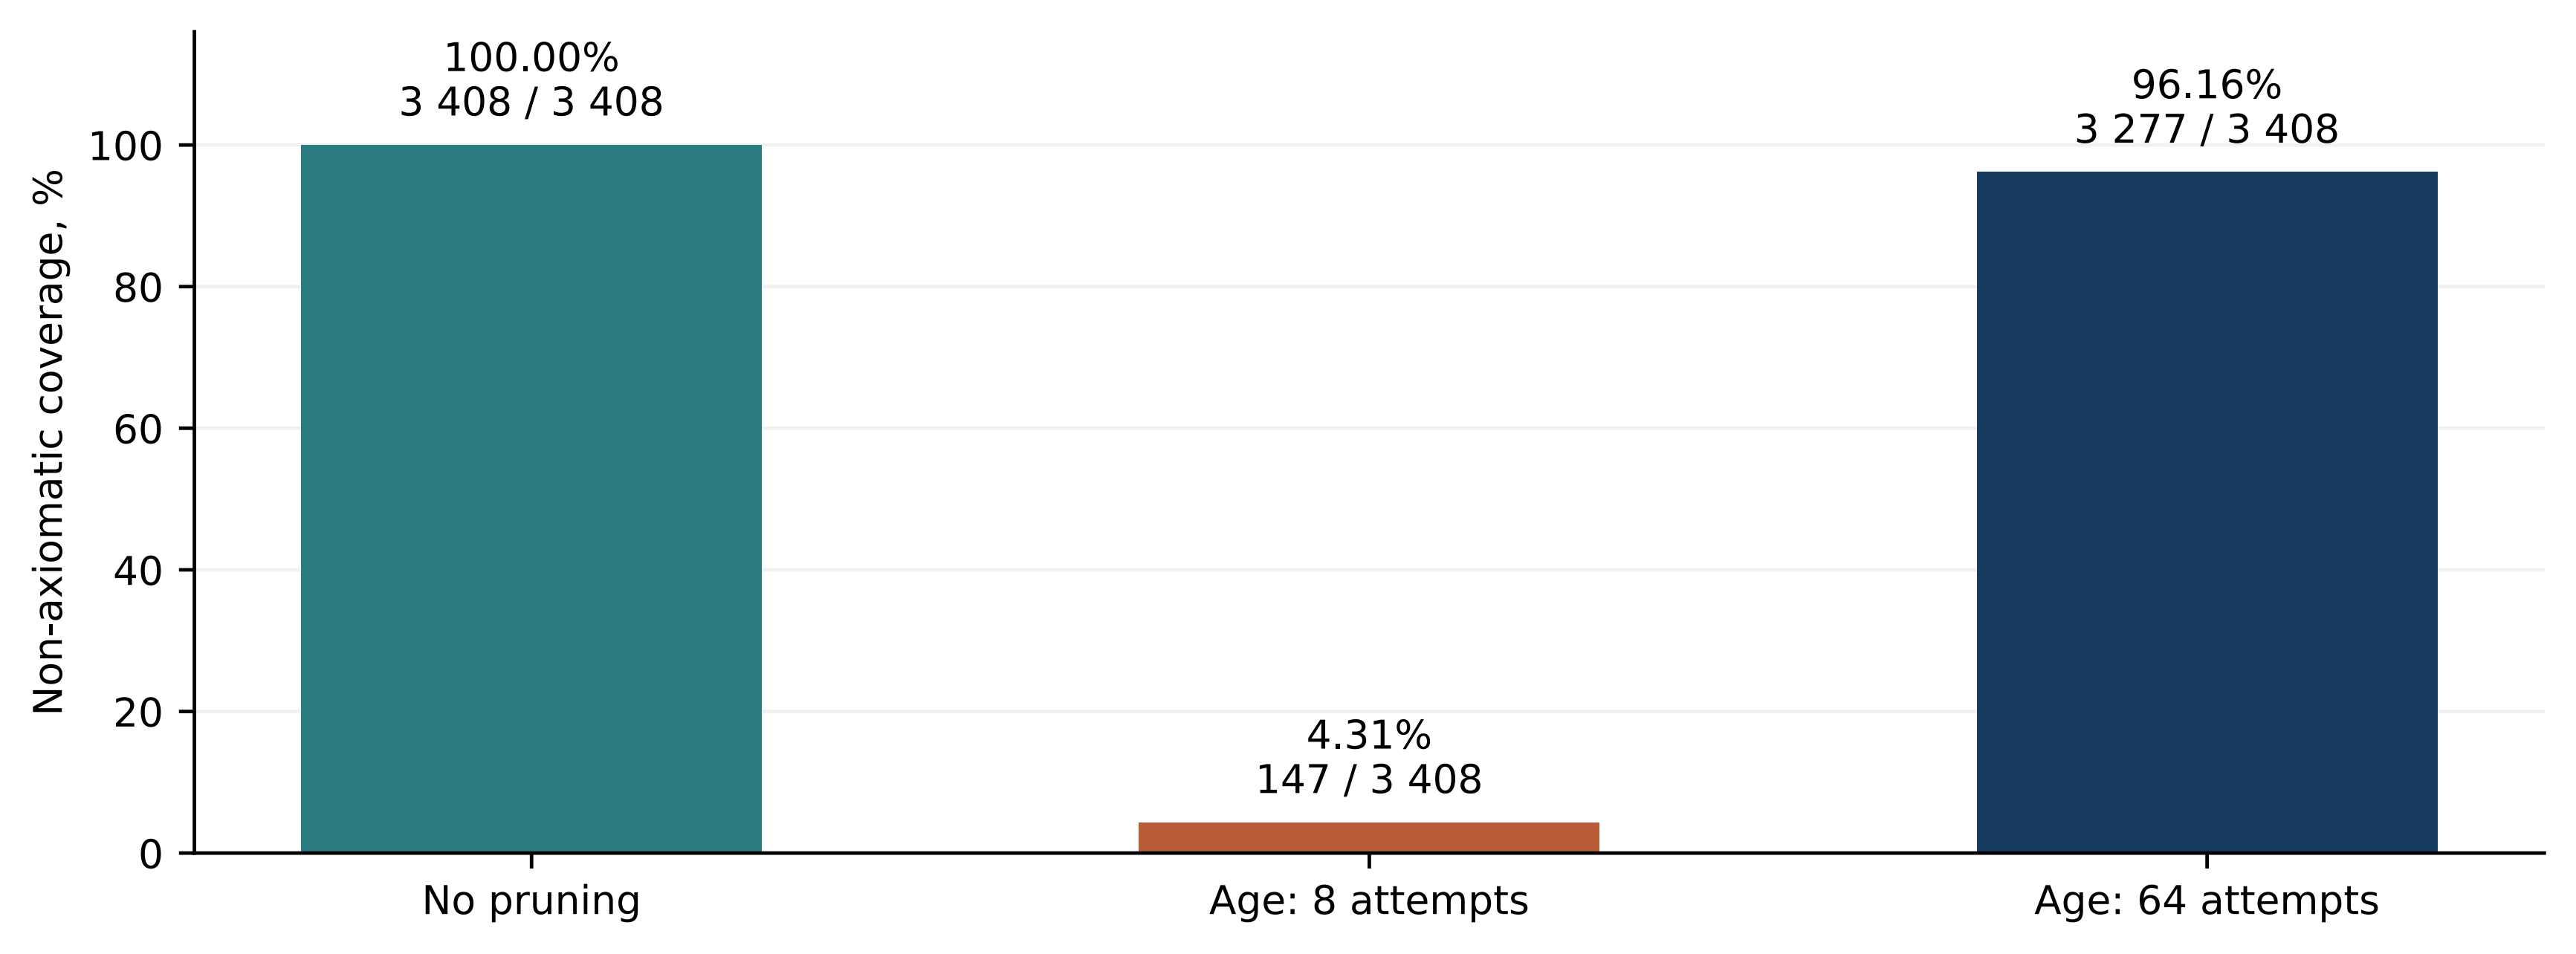
\includegraphics[width=\linewidth,height=.67\textheight,keepaspectratio]{Fig11.png}
\caption{Loss of non-axiomatic coverage under age pruning on the exact KSP benchmark. The plot shows arrival order with the same maximum attempt budget. The experiment excludes the cost of full generation}\label{fig:11}
\end{figure}

Additional paired experiments with five initial states confirmed pruning effects but no universal gain. Median differences in control coverage equal zero across four combinations of logical system and ranking, performance differences vary, and comparison of two utility versions changes selection sets without consistently improving coverage. The small number of replicates does not turn a zero difference into evidence of equivalence.

\subsubsection*{G.3.3. Preliminary transfer between epochs}\label{g.3.3.-preliminary-transfer-between-epochs}
\addcontentsline{toc}{subsubsection}{G.3.3. Preliminary transfer between epochs}

The old epoch algorithm ran a bounded growth window, chose 24 candidates, scored subsets in measurement mini-windows, and transferred four lemmas according to its contribution estimates. Costs included every measurement run and the final window. Both ranking and assessment outcomes used control statements, so this algorithm relied on targets (Table 23).

\begingroup
\small
\setlength{\tabcolsep}{3pt}
\renewcommand{\arraystretch}{1.13}

\begin{longtable}[]{@{}
  >{\raggedright\arraybackslash}p{(\linewidth - 4\tabcolsep) * \real{0.5409}}
  >{\raggedleft\arraybackslash}p{(\linewidth - 4\tabcolsep) * \real{0.1944}}
  >{\raggedleft\arraybackslash}p{(\linewidth - 4\tabcolsep) * \real{0.2647}}@{}}
\caption{Coverage and schema counts in the preliminary epoch-transfer comparison}\label{tab:23}\tabularnewline
\toprule\noalign{}
\begin{minipage}[b]{\linewidth}\raggedright
\textbf{Variant}
\end{minipage} & \begin{minipage}[b]{\linewidth}\raggedleft
\textbf{Coverage}
\end{minipage} & \begin{minipage}[b]{\linewidth}\raggedleft
\textbf{Total schema count}
\end{minipage} \\
\midrule\noalign{}
\endfirsthead
\toprule\noalign{}
\begin{minipage}[b]{\linewidth}\raggedright
\textbf{Variant}
\end{minipage} & \begin{minipage}[b]{\linewidth}\raggedleft
\textbf{Coverage}
\end{minipage} & \begin{minipage}[b]{\linewidth}\raggedleft
\textbf{Total schema count}
\end{minipage} \\
\midrule\noalign{}
\endhead
\bottomrule\noalign{}
\endlastfoot
One window, depth 16, width 64 & 11/14 & 58 612 \\
One window, depth 14, width 128 & 11/14 & 124 264 \\
One window, depth 20, width 64 & 11/14 & 82 791 \\
Three epochs with measurement-based selection & 11/14 & 911 417 \\
\end{longtable}

\endgroup

The cycle did not improve coverage and cost approximately 15.55 times as much as the cheapest single window in the table under the chosen counter. The measurement criterion accelerated early discovery of already accessible results but made no progress towards the remaining targets. This negative result concerns one policy, not every form of epoch-based construction.

Two later variants optimised proximity to targets that lacked coverage. Proximity scores rose but final coverage stayed at 11/14: trivial matches to a metavariable initially inflated the signal, and a broader problem persisted after that, since conclusion similarity ignored provability of the missing premise. These experiments support testing utility through actual outcomes rather than improvements in an internal score.

Transfer in the old code stores formulae that the next window introduces as local starting facts. The interface does not carry a complete inter-epoch certificate. The series therefore confirms the heuristic's computational behaviour but does not certify compliance with the skeleton requirements in Definition 1.

\subsubsection*{G.3.4. Graph skeletonisation}\label{g.3.4.-graph-skeletonisation}
\addcontentsline{toc}{subsubsection}{G.3.4. Graph skeletonisation}

A separate experiment removed terminal vertices from the ordinary projection, except axioms and control statements that it protected. It then examined strongly connected components, the subgraph of increasing depth, its transitive reduction, and structural twins. The following table records the resulting graph sizes (Table 24).

\begingroup
\small
\setlength{\tabcolsep}{3pt}
\renewcommand{\arraystretch}{1.13}

\begin{longtable}[]{@{}
  >{\raggedright\arraybackslash}p{(\linewidth - 8\tabcolsep) * \real{0.1714}}
  >{\raggedleft\arraybackslash}p{(\linewidth - 8\tabcolsep) * \real{0.1995}}
  >{\raggedleft\arraybackslash}p{(\linewidth - 8\tabcolsep) * \real{0.1619}}
  >{\raggedleft\arraybackslash}p{(\linewidth - 8\tabcolsep) * \real{0.2862}}
  >{\raggedleft\arraybackslash}p{(\linewidth - 8\tabcolsep) * \real{0.1810}}@{}}
\caption{Graph sizes after terminal pruning, depth restriction, and transitive reduction}\label{tab:24}\tabularnewline
\toprule\noalign{}
\begin{minipage}[b]{\linewidth}\raggedright
\textbf{Logical system}
\end{minipage} & \begin{minipage}[b]{\linewidth}\raggedleft
\textbf{Original vertices}
\end{minipage} & \begin{minipage}[b]{\linewidth}\raggedleft
\textbf{After pruning}
\end{minipage} & \begin{minipage}[b]{\linewidth}\raggedleft
\textbf{Edges in the depth subgraph}
\end{minipage} & \begin{minipage}[b]{\linewidth}\raggedleft
\textbf{After reduction}
\end{minipage} \\
\midrule\noalign{}
\endfirsthead
\toprule\noalign{}
\begin{minipage}[b]{\linewidth}\raggedright
\textbf{Logical system}
\end{minipage} & \begin{minipage}[b]{\linewidth}\raggedleft
\textbf{Original vertices}
\end{minipage} & \begin{minipage}[b]{\linewidth}\raggedleft
\textbf{After pruning}
\end{minipage} & \begin{minipage}[b]{\linewidth}\raggedleft
\textbf{Edges in the depth subgraph}
\end{minipage} & \begin{minipage}[b]{\linewidth}\raggedleft
\textbf{After reduction}
\end{minipage} \\
\midrule\noalign{}
\endhead
\bottomrule\noalign{}
\endlastfoot
Propositional & 14 301 & 357 & 13 958 & 8 647 \\
Modal & 11 520 & 392 & 15 310 & 7 926 \\
\end{longtable}

\endgroup

Removing 97.50\% and 96.60\% of vertices through this pruning shows strong selectivity relative to the set under protection. It does not imply retention of the same percentage of semantic content. Since control vertices influenced retention decisions, their reachability cannot provide an independent test of the skeleton.

Condensation almost entirely merged the remaining core: the largest components contained 356 of 357 and 391 of 392 vertices. This characterises a projection with repeated inferences, not the existence of one `main theorem' or interchangeability of every lemma. The result points to the need for hyperedges and certificates in meaningful skeletonisation.

\subsubsection*{G.3.5. Development of joint selection}\label{g.3.5.-development-of-joint-selection}
\addcontentsline{toc}{subsubsection}{G.3.5. Development of joint selection}

Before the main context-transfer test, two further development rounds each ran 24 trajectories on the same four source archives. The first compared one-layer joint selection with five controls, exceeded axiomatic growth in only one of four blocks, and failed the pre-specified rule for proceeding. Two random controls actually chose identical starting sets and therefore cannot represent independent selection mechanisms.

The second round compared joint one-layer selection with bounded three-layer novelty and reachability scores. The protocol's primary reachability variant lost to the axiom-only control in all four blocks, whereas the novelty variant exceeded the reachability variant in mean output and supplied the starting basis of the later context method; separate auditors replayed all witnesses and certificates from both rounds. Choosing that basis belongs to development rather than an independent test result.

Neither round enters the new method's confirmatory sample. Retaining them shows that context transfer arose after we inspected earlier results; only later groups with an unchanged policy and different sources support the transfer test. Completeness of the final certificates in the records does not convert heuristic exploration into a proof of optimality.

\section*{Appendix H. Prospective activation of proof fragments}\label{appendix-h.-prospective-activation-of-proof-fragments}
\addcontentsline{toc}{section}{Appendix H. Prospective activation of proof fragments}

\subsection*{H.1. Features and bounded probes}\label{h.1.-features-and-bounded-probes}
\addcontentsline{toc}{subsection}{H.1. Features and bounded probes}

Let \(s(v)\) count syntax-tree vertices, let \(h(v)\) denote the height of the stored first certificate, and let \(b(v)\) denote the maximum size among its stored ancestral formulae. The following recurrences define these last two quantities:

\[\fitdisplay{b(v) = max\left( s(v),\max_{p \in pa(v)}b(p) \right),\quad\quad h(v) = 1 + \max_{p \in pa(v)}h(p),}\]

with \(b(a) = s(a)\) and \(h(a) = 0\) for original axioms. These statistics describe the particular archived schematic witness. They do not minimise over alternative proofs or bound the peak of every fully instantiated expansion. Schematic MP may enlarge an original premise through substitution, so strict size decrease for a concrete detached conclusion does not imply decrease relative to the original major schema.

A deterministic hash of the seed, epoch, role, and vertex identifier orders active partners. The first 16 supply two oriented MP probes each. The operator keeps only separate diagnostic outcomes and counts \(a(v)\) attempted probes, \(m(v)\) admissible outcomes within \(L\), and \(n(v)\) distinct outcomes absent from the archive. Repeated outputs count once in \(n(v)\). The independent checker replays every logged probe through its own unifier; no diagnostic outcome enters the archive or receives theorem credit.

Let \(q(v)\) denote the positive marginal compression gain at dictionary selection. Let \(g(v)\) and \(r(v)\) denote cumulative new and duplicate direct credit. Define \(z(t) = log(1 + t)/(1 + log(1 + t))\). We use nine features

\[\fitdisplay{\begin{matrix}
x_{0} = 1,\quad\quad x_{1} = min\left( 1,\frac{log(b(v)/s(v))}{log(1 + L)} \right), \\
x_{2} = \frac{|vars(v)|}{\ell(v)},\quad\quad x_{3} = max(0,1 - s(v)/L), \\
x_{4} = \frac{n(v)}{max(1,a(v))},\quad\quad x_{5} = \frac{m(v)}{max(1,a(v))}, \\
x_{6} = \frac{g(v) + 1}{g(v) + r(v) + 2},\quad\quad x_{7} = z(max(0,q(v))), \\
x_{8} = z(h(v)),
\end{matrix}}\]

where \(\ell(v)\) counts leaves. All features fall in \(\lbrack 0,1\rbrack\) under the supported language and bounds. For ordinary comparator premises, \(q(v) = 0\). Compression controls do not execute probes that their activation rule does not use. Every method shares the same incremental certificate-peak and direct-credit instrumentation.

\subsection*{H.2. Analytical score and delayed linear model}\label{h.2.-analytical-score-and-delayed-linear-model}
\addcontentsline{toc}{subsection}{H.2. Analytical score and delayed linear model}

The analytical policy OP uses

\[\fitdisplay{S_{OP}(v) = \frac{n(v)}{max(1,a(v))}\left( 1 + log\frac{b(v)}{s(v)} \right)\left( \frac{1}{4} + max(0,1 - s(v)/L) \right)\frac{g(v) + 1}{g(v) + r(v) + 2}.}\]

The fixed term \(1/4\) allows a candidate at the size bound to retain a positive score. The probe result, rather than formula-size slack alone, tests admissibility of its immediate consequences. The score remains a heuristic because a larger certificate peak need not improve future search.

Li and colleagues \citep{Li2010LinUCB}, in \emph{A Contextual-Bandit Approach to Personalized News Article Recommendation}, introduced LinUCB for contextual-bandit problems. The following policy adapts its linear confidence index to delayed proof-reuse outcomes.

The linear policy OL starts with \(M_{0} = I_{9}\) and \(d_{0} = 0\), estimates \(\theta_{e} = M_{e}^{- 1}d_{e}\), and assigns the LinUCB-style index

\[\fitdisplay{S_{OL}(v) = \theta_{e}^{\top}x_{e}(v) + \frac{1}{2}\sqrt{x_{e}(v)^{\top}M_{e}^{- 1}x_{e}(v)}.}\]

At the end of a six-epoch observation window, it receives

\[\fitdisplay{y(v) = \frac{\Delta g(v) - \frac{1}{4}\Delta r(v)}{1 + \Delta g(v) + \Delta r(v)},\quad\quad M \leftarrow M + xx^{\top},\quad d \leftarrow d + yx.}\]

An inverse rank-one update implements the ridge step. Each new first-proof formula contributes \(1/k\) to each of its \(k\) distinct direct premises, so total attributed new credit equals the number of new results with premises. Rediscovery events use the same split. Splitting credit this way avoids counting one conclusion twice across its parents but does not identify causal value. The duplicate penalty measures events rather than elapsed time; failed unifications and size-filtered outputs do not enter this ratio. Whole-algorithm CPU includes their costs and supplies the primary endpoint.

The controller registers windows for selected library conclusions and up to eight sampled ordinary active premises. It freezes each feature vector at the window start, updates only after that window ends, and discards unfinished windows from training. Ordinary-premise outcomes provide cold-start observations. No historical fitted coefficients, unplayed-candidate labels, or human theorem targets enter the model. Outcomes remain correlated and policy dependent; the standard stationary linear-bandit regret theorem does not follow from this implementation.

At most one observation window remains pending per vertex. A later choice during that window does not reset its feature vector or clock, so an ordinary-premise window may span a subsequent library lease. The model estimates local observed yield rather than a separate causal response for every lease.

\subsection*{H.3. Slot rule and formal scope}\label{h.3.-slot-rule-and-formal-scope}
\addcontentsline{toc}{subsection}{H.3. Slot rule and formal scope}

At a decision epoch, the controller compares candidates with up to eight ordinary non-axiomatic premises outside the current dictionary. It computes both groups through the same score and sets

\[\fitdisplay{\tau_{e} = max\left( 0,{median}_{u \in C_{e}}S(u) \right).}\]

For an empty comparator set, set \(\tau_{e} = 0\). OP and OL admit candidates only when \(n(v) > 0\) and \(S(v) > \tau_{e}\text{.}\) They rank passing candidates by score and then identifier, and fill only vacant positions among four concurrent leases. Each lease expires after six epochs without automatic renewal. The existing generator applies its cooldown, layer width, and active-set bound, so a proposal does not guarantee immediate activation or six full epochs of actual exposure. Logged lifecycle events distinguish proposals from actual reactivation.

The current compression dictionary contains at most \(K\) conclusions. References to certificates of still-running leases may add up to four more, so the combined library support contains at most \(K + 4\) identifiers. These references do not enlarge the four-lease or 128-active-premise bounds. The common archive retains their certificates throughout.

\textbf{Proposition H.1 (empty activation and fixed epochs).} Consider two runs with identical initial proofs, generation rules, canonicalisation, scheduling, bounds, and epoch clocks. Suppose the added controller writes only private statistics and never changes search state or activates a candidate. At every completed epoch, both runs then produce the same archive and active/passive search sets. This statement imposes no equality of elapsed CPU or of the epoch that search reaches within a CPU budget.

\textbf{Proof.} The initial archives and search sets coincide by assumption. Suppose they coincide at the start of an epoch. The same scheduler and rule applications then yield the same ordered conclusions, duplicate events, and first proofs. The ordinary retention and activation procedures receive the same state and make the same changes. Private statistics and probes write no search state, and the empty activation operator contributes no further change. Thus the next completed epoch preserves equality, and induction gives the claim. Additional computations can change elapsed CPU, so the argument provides no fixed-time equality. \(\square\)

Certificate soundness follows under the same assumptions as Appendix B: an archived certificate already supports every activated conclusion, references preserve its original dependency order, and the unchanged kernel checks each subsequent inference. A learned score changes access to premises rather than their proof status. Neither this fact nor Proposition H.1 guarantees completeness, faster search, a minimal skeleton, or absence of memory stops.

Probes pair a candidate with active partners without enforcing the next-layer frontier condition. Retaining an already active conclusion can preserve access without rescheduling every probed pairing. The observed outcomes test this particular one-step proxy rather than its ability to predict all future rule applications.

\subsection*{H.4. Protocol and reproducibility}\label{h.4.-protocol-and-reproducibility}
\addcontentsline{toc}{subsection}{H.4. Protocol and reproducibility}

The development pilot comprises 24 trajectories: four policies, three logic--size strata, and scheduler states 7301--7302. The strata use propositional logic at \(L = 25\) and \(L = 200\), and normal modal K at \(L = 25\). Each trajectory receives five CPU-seconds, with nested readings at \(5/3\) and five seconds. A separate panel freezes the same parameters on states 7401--7404 and reads at 10 and 30 CPU-seconds. A further 24-trajectory pilot uses states 7501--7502 and a dictionary pool of 16 in every policy; it assesses capacity separately and does not enter the 48-trajectory confirmation.

OB stores the compression dictionary without activation. OA6 grants unconditional fixed leases in decreasing order of marginal compression gain. OP and OL use the threshold in Section H.3. Every policy permits four concurrent leases, 128 derived active premises, and 4,096 passive candidates, with width 32, six-epoch active retention, four-epoch passive retention, a two-epoch cooldown, and at most eight rediscovery returns per layer. Dictionary decisions occur at four-epoch intervals when that epoch adds new formulae, using the last 128 first proofs and at most 16 compression candidates. The principal panels keep the dictionary pool at four. OA6 differs from the historical OA through the renewal rule, so historical results do not replace concurrent controls.

Every run starts from original axioms and charges generation, policy computation, certificate merge and checking, measurements, and journal writes to one process-CPU budget. The program checks a soft 1.5 GiB memory guard between layers, caps the archive at 500,000 formulae, and stops after at most 4,096 epochs. Only fully committed layers within budget receive endpoint credit. The protocol records all stops, late commits, and unfinished observations. Seeds vary scheduling within a fixed formal configuration rather than sampling independent mathematical theories.

The verifier independently checks every first proof, canonical uniqueness, active/support bounds, first-certificate peak and height, allocated new credit, and probe outcome. It also replays compression choice, delayed ridge updates, score thresholds, and lease clocks. Rediscovery counts remain instrumented operational measurements, since first-proof provenance does not preserve every duplicate derivation. The primary novel-formula counts therefore rely on independently replayable certificates rather than the reward log alone.

The implementation resides in \path{prospective_policy.py}, \path{prospective_engine.py}, \path{prospective_suite.py}, and \path{prospective_report.py}. The launcher \path{run_article1_prospective.sh} supports \path{prepare}, \path{run}, \path{audit}, \path{status}, and \path{report}. Before the runs start, the preparation step freezes the source tree, task order, parameters, and content hashes. Each worker writes a separate append-only journal. The independent audit retains failed cells and rejects configuration or content drift.

\subsection*{H.5. Results and scope of the comparison}\label{h.5.-results-and-scope-of-the-comparison}
\addcontentsline{toc}{subsection}{H.5. Results and scope of the comparison}

All 96 trajectories across the three new panels pass independent audit, which checks 8,270 checkpoints and 3,863,642 first-proof records. The last count sums records across trajectories rather than distinct theorems in their union.

\subsubsection*{H.5.1. Pilot}\label{h.5.1.-pilot}
\addcontentsline{toc}{subsubsection}{H.5.1. Pilot}

Table 25 reports pilot ratios and positive pairs at each recorded budget.

\begingroup
\small
\setlength{\tabcolsep}{3pt}
\renewcommand{\arraystretch}{1.13}

\begin{longtable}[]{@{}
  >{\raggedright\arraybackslash}p{(\linewidth - 10\tabcolsep) * \real{0.1618}}
  >{\raggedleft\arraybackslash}p{(\linewidth - 10\tabcolsep) * \real{0.1618}}
  >{\raggedleft\arraybackslash}p{(\linewidth - 10\tabcolsep) * \real{0.1618}}
  >{\raggedleft\arraybackslash}p{(\linewidth - 10\tabcolsep) * \real{0.1618}}
  >{\raggedleft\arraybackslash}p{(\linewidth - 10\tabcolsep) * \real{0.1618}}
  >{\raggedright\arraybackslash}p{(\linewidth - 10\tabcolsep) * \real{0.1911}}@{}}
\caption{Prospective-policy ratios and positive pairs in the pilot}\label{tab:25}\tabularnewline
\toprule\noalign{}
\begin{minipage}[b]{\linewidth}\raggedright
\textbf{Stratum}
\end{minipage} & \begin{minipage}[b]{\linewidth}\raggedleft
\textbf{CPU, s}
\end{minipage} & \begin{minipage}[b]{\linewidth}\raggedleft
\textbf{OA6/OB}
\end{minipage} & \begin{minipage}[b]{\linewidth}\raggedleft
\textbf{OP/OB}
\end{minipage} & \begin{minipage}[b]{\linewidth}\raggedleft
\textbf{OL/OB}
\end{minipage} & \begin{minipage}[b]{\linewidth}\raggedright
\textbf{Positive OP; OL}
\end{minipage} \\
\midrule\noalign{}
\endfirsthead
\toprule\noalign{}
\begin{minipage}[b]{\linewidth}\raggedright
\textbf{Stratum}
\end{minipage} & \begin{minipage}[b]{\linewidth}\raggedleft
\textbf{CPU, s}
\end{minipage} & \begin{minipage}[b]{\linewidth}\raggedleft
\textbf{OA6/OB}
\end{minipage} & \begin{minipage}[b]{\linewidth}\raggedleft
\textbf{OP/OB}
\end{minipage} & \begin{minipage}[b]{\linewidth}\raggedleft
\textbf{OL/OB}
\end{minipage} & \begin{minipage}[b]{\linewidth}\raggedright
\textbf{Positive OP; OL}
\end{minipage} \\
\midrule\noalign{}
\endhead
\bottomrule\noalign{}
\endlastfoot
Prop. 25 & 1.67 & -0.9\% & +0.0\% & +0.5\% & 0/2; 1/2 \\
Prop. 25 & 5.00 & +8.2\% & -3.3\% & -5.8\% & 0/2; 0/2 \\
Prop. 200 & 1.67 & -1.1\% & +0.0\% & -0.0\% & 0/2; 0/2 \\
Prop. 200 & 5.00 & +3.8\% & +0.0\% & +3.9\% & 0/2; 1/2 \\
Modal K 25 & 1.67 & +0.2\% & -3.0\% & +0.8\% & 1/2; 2/2 \\
Modal K 25 & 5.00 & -2.4\% & -7.3\% & -6.9\% & 0/2; 0/2 \\
\end{longtable}

\endgroup

\subsubsection*{H.5.2. New scheduler states}\label{h.5.2.-new-scheduler-states}
\addcontentsline{toc}{subsubsection}{H.5.2. New scheduler states}

Table 26 reports the same outcomes on the four new scheduler states.

\begingroup
\small
\setlength{\tabcolsep}{3pt}
\renewcommand{\arraystretch}{1.13}

\begin{longtable}[]{@{}
  >{\raggedright\arraybackslash}p{(\linewidth - 10\tabcolsep) * \real{0.1618}}
  >{\raggedleft\arraybackslash}p{(\linewidth - 10\tabcolsep) * \real{0.1618}}
  >{\raggedleft\arraybackslash}p{(\linewidth - 10\tabcolsep) * \real{0.1618}}
  >{\raggedleft\arraybackslash}p{(\linewidth - 10\tabcolsep) * \real{0.1618}}
  >{\raggedleft\arraybackslash}p{(\linewidth - 10\tabcolsep) * \real{0.1618}}
  >{\raggedright\arraybackslash}p{(\linewidth - 10\tabcolsep) * \real{0.1911}}@{}}
\caption{Prospective-policy ratios and positive pairs on four new scheduler states}\label{tab:26}\tabularnewline
\toprule\noalign{}
\begin{minipage}[b]{\linewidth}\raggedright
\textbf{Stratum}
\end{minipage} & \begin{minipage}[b]{\linewidth}\raggedleft
\textbf{CPU, s}
\end{minipage} & \begin{minipage}[b]{\linewidth}\raggedleft
\textbf{OA6/OB}
\end{minipage} & \begin{minipage}[b]{\linewidth}\raggedleft
\textbf{OP/OB}
\end{minipage} & \begin{minipage}[b]{\linewidth}\raggedleft
\textbf{OL/OB}
\end{minipage} & \begin{minipage}[b]{\linewidth}\raggedright
\textbf{Positive OP; OL}
\end{minipage} \\
\midrule\noalign{}
\endfirsthead
\toprule\noalign{}
\begin{minipage}[b]{\linewidth}\raggedright
\textbf{Stratum}
\end{minipage} & \begin{minipage}[b]{\linewidth}\raggedleft
\textbf{CPU, s}
\end{minipage} & \begin{minipage}[b]{\linewidth}\raggedleft
\textbf{OA6/OB}
\end{minipage} & \begin{minipage}[b]{\linewidth}\raggedleft
\textbf{OP/OB}
\end{minipage} & \begin{minipage}[b]{\linewidth}\raggedleft
\textbf{OL/OB}
\end{minipage} & \begin{minipage}[b]{\linewidth}\raggedright
\textbf{Positive OP; OL}
\end{minipage} \\
\midrule\noalign{}
\endhead
\bottomrule\noalign{}
\endlastfoot
Prop. 25 & 10.00 & +14.0\% & -2.4\% & +2.2\% & 1/4; 2/4 \\
Prop. 25 & 30.00 & +19.5\% & +16.6\% & +17.0\% & 3/4; 2/4 \\
Prop. 200 & 10.00 & -1.2\% & -3.0\% & -0.2\% & 0/4; 2/4 \\
Prop. 200 & 30.00 & -5.9\% & -0.7\% & -11.0\% & 3/4; 1/4 \\
Modal K 25 & 10.00 & +9.9\% & -2.5\% & -1.9\% & 1/4; 2/4 \\
Modal K 25 & 30.00 & +30.6\% & +10.7\% & +10.9\% & 4/4; 3/4 \\
\end{longtable}

\endgroup

We report every policy-minus-OB difference in new-formula counts, in source order 7401--7404 (Table 27).

\begingroup
\small
\setlength{\tabcolsep}{3pt}
\renewcommand{\arraystretch}{1.13}

\begin{longtable}[]{@{}
  >{\raggedright\arraybackslash}p{(\linewidth - 8\tabcolsep) * \real{0.1298}}
  >{\raggedleft\arraybackslash}p{(\linewidth - 8\tabcolsep) * \real{0.1297}}
  >{\raggedright\arraybackslash}p{(\linewidth - 8\tabcolsep) * \real{0.2561}}
  >{\raggedright\arraybackslash}p{(\linewidth - 8\tabcolsep) * \real{0.2352}}
  >{\raggedright\arraybackslash}p{(\linewidth - 8\tabcolsep) * \real{0.2492}}@{}}
\caption{Per-state new-formula differences from the passive-library control on states 7401--7404}\label{tab:27}\tabularnewline
\toprule\noalign{}
\begin{minipage}[b]{\linewidth}\raggedright
\textbf{Stratum}
\end{minipage} & \begin{minipage}[b]{\linewidth}\raggedleft
\textbf{CPU, s}
\end{minipage} & \begin{minipage}[b]{\linewidth}\raggedright
\textbf{OA6}
\end{minipage} & \begin{minipage}[b]{\linewidth}\raggedright
\textbf{OP}
\end{minipage} & \begin{minipage}[b]{\linewidth}\raggedright
\textbf{OL}
\end{minipage} \\
\midrule\noalign{}
\endfirsthead
\toprule\noalign{}
\begin{minipage}[b]{\linewidth}\raggedright
\textbf{Stratum}
\end{minipage} & \begin{minipage}[b]{\linewidth}\raggedleft
\textbf{CPU, s}
\end{minipage} & \begin{minipage}[b]{\linewidth}\raggedright
\textbf{OA6}
\end{minipage} & \begin{minipage}[b]{\linewidth}\raggedright
\textbf{OP}
\end{minipage} & \begin{minipage}[b]{\linewidth}\raggedright
\textbf{OL}
\end{minipage} \\
\midrule\noalign{}
\endhead
\bottomrule\noalign{}
\endlastfoot
Prop. 25 & 10 & +3812, +3253, +662, +4929 & -1260, -408, +1052, -1513 & -320, +1018, -171, +1430 \\
Prop. 25 & 30 & +11609, +22919, -4658, +11101 & -904, +25963, +2258, +7570 & -8440, +38422, +6273, -534 \\
Prop. 200 & 10 & -2222, +451, -295, +545 & -2175, -1397, +0, -131 & -2078, +1340, -1148, +1631 \\
Prop. 200 & 30 & -9186, +1277, -4052, -7104 & +904, +4402, +2393, -9817 & -19477, +1022, -12886, -3997 \\
Modal K 25 & 10 & -123, +2205, +2956, +4016 & +1402, -982, -2444, -217 & +1908, -357, -3733, +447 \\
Modal K 25 & 30 & -364, +23819, +16992, +26457 & +9643, +1192, +6901, +5572 & +9099, +5229, -70, +9512 \\
\end{longtable}

\endgroup

\subsubsection*{H.5.3. Pool capacity 16}\label{h.5.3.-pool-capacity-16}
\addcontentsline{toc}{subsubsection}{H.5.3. Pool capacity 16}

Table 28 reports the comparison with a pool capacity of 16 at each recorded budget.

\begingroup
\small
\setlength{\tabcolsep}{3pt}
\renewcommand{\arraystretch}{1.13}

\begin{longtable}[]{@{}
  >{\raggedright\arraybackslash}p{(\linewidth - 10\tabcolsep) * \real{0.1618}}
  >{\raggedleft\arraybackslash}p{(\linewidth - 10\tabcolsep) * \real{0.1618}}
  >{\raggedleft\arraybackslash}p{(\linewidth - 10\tabcolsep) * \real{0.1618}}
  >{\raggedleft\arraybackslash}p{(\linewidth - 10\tabcolsep) * \real{0.1618}}
  >{\raggedleft\arraybackslash}p{(\linewidth - 10\tabcolsep) * \real{0.1618}}
  >{\raggedright\arraybackslash}p{(\linewidth - 10\tabcolsep) * \real{0.1911}}@{}}
\caption{Prospective-policy ratios and positive pairs with pool capacity 16}\label{tab:28}\tabularnewline
\toprule\noalign{}
\begin{minipage}[b]{\linewidth}\raggedright
\textbf{Stratum}
\end{minipage} & \begin{minipage}[b]{\linewidth}\raggedleft
\textbf{CPU, s}
\end{minipage} & \begin{minipage}[b]{\linewidth}\raggedleft
\textbf{OA6/OB}
\end{minipage} & \begin{minipage}[b]{\linewidth}\raggedleft
\textbf{OP/OB}
\end{minipage} & \begin{minipage}[b]{\linewidth}\raggedleft
\textbf{OL/OB}
\end{minipage} & \begin{minipage}[b]{\linewidth}\raggedright
\textbf{Positive OP; OL}
\end{minipage} \\
\midrule\noalign{}
\endfirsthead
\toprule\noalign{}
\begin{minipage}[b]{\linewidth}\raggedright
\textbf{Stratum}
\end{minipage} & \begin{minipage}[b]{\linewidth}\raggedleft
\textbf{CPU, s}
\end{minipage} & \begin{minipage}[b]{\linewidth}\raggedleft
\textbf{OA6/OB}
\end{minipage} & \begin{minipage}[b]{\linewidth}\raggedleft
\textbf{OP/OB}
\end{minipage} & \begin{minipage}[b]{\linewidth}\raggedleft
\textbf{OL/OB}
\end{minipage} & \begin{minipage}[b]{\linewidth}\raggedright
\textbf{Positive OP; OL}
\end{minipage} \\
\midrule\noalign{}
\endhead
\bottomrule\noalign{}
\endlastfoot
Prop. 25 & 1.67 & +0.1\% & +0.0\% & +0.1\% & 0/2; 1/2 \\
Prop. 25 & 5.00 & -4.7\% & -3.3\% & -6.6\% & 0/2; 0/2 \\
Prop. 200 & 1.67 & -2.4\% & +0.0\% & -1.3\% & 0/2; 0/2 \\
Prop. 200 & 5.00 & -1.5\% & +0.0\% & -4.4\% & 0/2; 0/2 \\
Modal K 25 & 1.67 & +1.0\% & -0.1\% & -0.3\% & 0/2; 0/2 \\
Modal K 25 & 5.00 & +0.2\% & -3.3\% & +1.6\% & 0/2; 1/2 \\
\end{longtable}

\endgroup

\subsubsection*{H.5.4. Policy costs and controller events}\label{h.5.4.-policy-costs-and-controller-events}
\addcontentsline{toc}{subsubsection}{H.5.4. Policy costs and controller events}

Table 29 records policy costs and controller events separately from formula output.

\begingroup
\small
\setlength{\tabcolsep}{3pt}
\renewcommand{\arraystretch}{1.13}

\begin{longtable}[]{@{}
  >{\raggedright\arraybackslash}p{(\linewidth - 8\tabcolsep) * \real{0.1978}}
  >{\raggedright\arraybackslash}p{(\linewidth - 8\tabcolsep) * \real{0.1978}}
  >{\raggedleft\arraybackslash}p{(\linewidth - 8\tabcolsep) * \real{0.2089}}
  >{\raggedleft\arraybackslash}p{(\linewidth - 8\tabcolsep) * \real{0.1978}}
  >{\raggedleft\arraybackslash}p{(\linewidth - 8\tabcolsep) * \real{0.1978}}@{}}
\caption{Policy CPU costs, leases, and controller updates in the prospective series}\label{tab:29}\tabularnewline
\toprule\noalign{}
\begin{minipage}[b]{\linewidth}\raggedright
\textbf{Stratum}
\end{minipage} & \begin{minipage}[b]{\linewidth}\raggedright
\textbf{Policy}
\end{minipage} & \begin{minipage}[b]{\linewidth}\raggedleft
\textbf{Policy CPU, s}
\end{minipage} & \begin{minipage}[b]{\linewidth}\raggedleft
\textbf{Leases}
\end{minipage} & \begin{minipage}[b]{\linewidth}\raggedleft
\textbf{Updates}
\end{minipage} \\
\midrule\noalign{}
\endfirsthead
\toprule\noalign{}
\begin{minipage}[b]{\linewidth}\raggedright
\textbf{Stratum}
\end{minipage} & \begin{minipage}[b]{\linewidth}\raggedright
\textbf{Policy}
\end{minipage} & \begin{minipage}[b]{\linewidth}\raggedleft
\textbf{Policy CPU, s}
\end{minipage} & \begin{minipage}[b]{\linewidth}\raggedleft
\textbf{Leases}
\end{minipage} & \begin{minipage}[b]{\linewidth}\raggedleft
\textbf{Updates}
\end{minipage} \\
\midrule\noalign{}
\endhead
\bottomrule\noalign{}
\endlastfoot
Prop. 25 & OB & 0.855 & 0.00 & 0.00 \\
Prop. 25 & OA6 & 0.775 & 96.50 & 0.00 \\
Prop. 25 & OP & 1.225 & 29.50 & 0.00 \\
Prop. 25 & OL & 1.144 & 23.75 & 323.00 \\
Prop. 200 & OB & 0.256 & 0.00 & 0.00 \\
Prop. 200 & OA6 & 0.241 & 26.00 & 0.00 \\
Prop. 200 & OP & 0.459 & 13.00 & 0.00 \\
Prop. 200 & OL & 0.445 & 16.25 & 95.50 \\
Modal K 25 & OB & 0.690 & 0.00 & 0.00 \\
Modal K 25 & OA6 & 0.830 & 104.00 & 0.00 \\
Modal K 25 & OP & 1.371 & 29.25 & 0.00 \\
Modal K 25 & OL & 1.385 & 27.75 & 389.75 \\
\end{longtable}

\endgroup

Policy CPU reports the mean CPU time spent selecting and measuring over credited commits through 30 seconds. Leases count issued proposals; updates refer to the complete trajectory, including late finalisation, rather than a budgeted endpoint. The stop log records 36 \path{cpu_frontier}, eight \path{finalization_over_budget}, and four \path{total_cpu} outcomes.

Failure to improve does not rule out every prospective policy. The test concerns these features, one-step local probes, lease duration, and observational reward. A short conclusion and a large certificate peak need not yield new consequences; choosing an already active formula may only extend its retention. The CPU budget charges the costs of predicting yield but does not isolate an individual feature effect. Such a claim would require feature ablations or matched branches from a common state.

pilot: \path{output/article1_prospective_pilot_20261014_v1}.

Protocol SHA-256:

\path{f6bc71355e41a2a967bccf0f4b573eca956d59fa4ebb693ec7ba60ffba464886}.

Audit SHA-256:

\path{ade24c30dde1cc6d0c985fd3a6e2251ea64dcf9e7037e2fe187afe5ec8d91818}.

confirmation: \path{output/article1_prospective_confirmation_20261014_v1}.

Protocol SHA-256:

\path{88fd04cfbea0fc6955136eba6a9e7451dc0b26f80efc3586bd276807fbe88280}.

Audit SHA-256:

\path{48def42d1fb3c4924b7710dfd05b53b1bc4132707a5b18ed4ea7016eda844683}.

pool16: \path{output/article1_prospective_pool16_20261014_v1}.

Protocol SHA-256:

\path{787f503f4160a357731619902e8965a5dfdfa0d691200a714078cee5e01a3a75}.

Audit SHA-256:

\path{27b8968c3e09cbcfbabbf6e86ed13004f0208e08d02d79d91b4f00dffe6d15a2}.

\subsection*{H.6. Matches with the human benchmark}\label{h.6.-matches-with-the-human-benchmark}
\addcontentsline{toc}{subsection}{H.6. Matches with the human benchmark}

After all searches and audits finished, we compared their results exactly with the previous 108 short closed propositional statements. The generator, its features, and its reward never used this set. The table reports means over four states at 30 CPU-seconds and treats the current compression dictionary separately from the active set and archive (Table 30).

\begingroup
\small
\setlength{\tabcolsep}{3pt}
\renewcommand{\arraystretch}{1.13}

\begin{longtable}[]{@{}
  >{\raggedleft\arraybackslash}p{(\linewidth - 8\tabcolsep) * \real{0.2000}}
  >{\raggedright\arraybackslash}p{(\linewidth - 8\tabcolsep) * \real{0.2000}}
  >{\raggedleft\arraybackslash}p{(\linewidth - 8\tabcolsep) * \real{0.2000}}
  >{\raggedleft\arraybackslash}p{(\linewidth - 8\tabcolsep) * \real{0.2000}}
  >{\raggedleft\arraybackslash}p{(\linewidth - 8\tabcolsep) * \real{0.2000}}@{}}
\caption{Exact human-reference matches in archives, active sets, and compression dictionaries}\label{tab:30}\tabularnewline
\toprule\noalign{}
\begin{minipage}[b]{\linewidth}\raggedleft
\textbf{Bound}
\end{minipage} & \begin{minipage}[b]{\linewidth}\raggedright
\textbf{Policy}
\end{minipage} & \begin{minipage}[b]{\linewidth}\raggedleft
\textbf{Archive}
\end{minipage} & \begin{minipage}[b]{\linewidth}\raggedleft
\textbf{Active set}
\end{minipage} & \begin{minipage}[b]{\linewidth}\raggedleft
\textbf{Dictionary}
\end{minipage} \\
\midrule\noalign{}
\endfirsthead
\toprule\noalign{}
\begin{minipage}[b]{\linewidth}\raggedleft
\textbf{Bound}
\end{minipage} & \begin{minipage}[b]{\linewidth}\raggedright
\textbf{Policy}
\end{minipage} & \begin{minipage}[b]{\linewidth}\raggedleft
\textbf{Archive}
\end{minipage} & \begin{minipage}[b]{\linewidth}\raggedleft
\textbf{Active set}
\end{minipage} & \begin{minipage}[b]{\linewidth}\raggedleft
\textbf{Dictionary}
\end{minipage} \\
\midrule\noalign{}
\endhead
\bottomrule\noalign{}
\endlastfoot
25 & OB & 19.25 & 2.75 & 0 \\
25 & OA6 & 20 & 4.5 & 0 \\
25 & OP & 21.5 & 5 & 0 \\
25 & OL & 19 & 5 & 0 \\
200 & OB & 19 & 4.5 & 0 \\
200 & OA6 & 19 & 5 & 0.25 \\
200 & OP & 19 & 5.25 & 0.25 \\
200 & OL & 19 & 5 & 0.5 \\
\end{longtable}

\endgroup

At size 25, OP reaches the highest mean archive-match count although OA6 yields more new formulae. At size 200, all four archives average 19 matches. This divergence shows why we must assess the skeleton's mathematical content alongside canonical-formula counts. The 108 statements do not represent a complete human reference, and their proof intermediates may exceed the imposed size bound; modal runs do not enter this comparison.

The diagnostic file lists found and missing labels separately for every trajectory and both budgets. Earlier experiments already used this set, which supplies no independent holdout. Reference SHA-256: \path{9b235fc0788b1bf22fad4631f43627bd78da53ef5ef0bb4ba28117ea16c436b2}. Diagnostic SHA-256: \path{c8aed16e1f083b4ba81db6d0de0e7da1e08dc6b142a8b9ab9a9e4a01faf082ed}.

\section*{Appendix I. Continuation and Pareto evidence}\label{appendix-i.-continuation-and-pareto-evidence}
\addcontentsline{toc}{section}{Appendix I. Continuation and Pareto evidence}

\subsection*{I.1. Frozen pair selection and replay panel}\label{i.1.-frozen-pair-selection-and-replay-panel}
\addcontentsline{toc}{subsection}{I.1. Frozen pair selection and replay panel}

The panel crosses six policies, three logic--size regimes, and scheduler states 8701--8708. The policies admit all compatible pairs, a random half, or a learned half; the latter two also run with deferred replay, and a sixth variant retains a learned quarter with replay. All conditions use the same initial axioms, canonical forms, model files, lifecycle, and certificate checker within a regime. The original training archives supply labels and weights; this panel introduces no human theorem targets or new model fitting.

Every source receives nominal readings at 60, 180, and 600 CPU-seconds. Each reading supplies anchor caps 4, 16, and 64, and each resulting package receives a separate neutral continuation with readings at 10, 30, and 60 CPU-seconds. This design produces 144 sources, 1,296 continuations, and 3,888 continuation readings. Nested readings and repeated source packages do not count as independent trajectories. The prespecified primary endpoint uses source ceiling 180, cap 16, and continuation 30; the main text retains that endpoint rather than selecting a more favourable secondary cell.

The model describes only already available premises. A fixed share of exploratory candidates accompanies learned ranking, and admitted pairs preserve the generator's traversal order. Replay stores up to 32,768 skipped pairs, attempts up to 128 ready pairs per epoch, and reserves at most four ordinary premise slots. Queue overflow counts rejected offers rather than distinct lost pairs or theorems. None of these finite quotas guarantees fair exhaustive enumeration.

The independent cluster checker verifies 24 logic--state blocks. Local checks compare all 229,221 journal-chain files against those checked records and replay every one of the 1,296 exported proof-backed packages. Those package replays traverse 172,522 support records with repetitions across packages. Transport integrity binds the downloaded large journals to the cluster audit; it does not constitute another local logical replay of every elementary proof in those journals.

The reported source, selection, and continuation components total 27.17 CPU-hours; including the two audit stages gives 35.02 CPU-hours, excluding some startup and orchestration. Earlier training and preparation cost 37.79 CPU-seconds once. These components describe measured process work rather than the SLURM bill or a hardware-independent complexity measure. At the credited endpoints, memory guards and incomplete layers can leave actual CPU below the assigned ceiling.

Frozen protocol SHA-256:

\path{cbab9bc7eb7c2b14d4d604341898cc101c6f4e8a93e61d971d7f2b1c20f11905}.

Final cluster audit SHA-256:

\path{fe91c9adc86c5aaf92349ea5beee7846ddda2af44226827ad681d61977ac1357}.

\subsection*{I.2. Finite grid and Pareto coordinates}\label{i.2.-finite-grid-and-pareto-coordinates}
\addcontentsline{toc}{subsection}{I.2. Finite grid and Pareto coordinates}

The new descriptive Pareto check uses only source ceiling 180 and continuation horizon 30. Each regime contains six policies at three anchor caps, hence 18 mean triples across eight schedules. The coordinates use credited chain CPU, complete package bytes, and new schemata outside the concurrent source union and old training. We recompute dominance from the existing aggregate records; no search, hypothesis test, or selection of favourable states follows this check.

The frontiers contain five settings at propositional size 25, seven at propositional size 200, and five at modal size 25. The table lists their mean coordinates. Names H and Q denote learned half and quarter selection, R denotes random half selection, and +replay denotes deferred attempts. The absence of a policy from this finite mean frontier does not imply dominance at every schedule, every cost, or another horizon (Table 31).

\begingroup
\small
\setlength{\tabcolsep}{3pt}
\renewcommand{\arraystretch}{1.13}

\begin{longtable}[]{@{}
  >{\raggedright\arraybackslash}p{(\linewidth - 10\tabcolsep) * \real{0.1650}}
  >{\raggedright\arraybackslash}p{(\linewidth - 10\tabcolsep) * \real{0.1651}}
  >{\raggedleft\arraybackslash}p{(\linewidth - 10\tabcolsep) * \real{0.1651}}
  >{\raggedleft\arraybackslash}p{(\linewidth - 10\tabcolsep) * \real{0.1651}}
  >{\raggedleft\arraybackslash}p{(\linewidth - 10\tabcolsep) * \real{0.1744}}
  >{\raggedleft\arraybackslash}p{(\linewidth - 10\tabcolsep) * \real{0.1651}}@{}}
\caption{Mean CPU, package bytes, and new schemata for the finite three-coordinate Pareto frontiers}\label{tab:31}\tabularnewline
\toprule\noalign{}
\begin{minipage}[b]{\linewidth}\raggedright
\textbf{Regime}
\end{minipage} & \begin{minipage}[b]{\linewidth}\raggedright
\textbf{Policy}
\end{minipage} & \begin{minipage}[b]{\linewidth}\raggedleft
\textbf{Anchor cap}
\end{minipage} & \begin{minipage}[b]{\linewidth}\raggedleft
\textbf{Chain CPU s}
\end{minipage} & \begin{minipage}[b]{\linewidth}\raggedleft
\textbf{Package bytes}
\end{minipage} & \begin{minipage}[b]{\linewidth}\raggedleft
\textbf{New schemata}
\end{minipage} \\
\midrule\noalign{}
\endfirsthead
\toprule\noalign{}
\begin{minipage}[b]{\linewidth}\raggedright
\textbf{Regime}
\end{minipage} & \begin{minipage}[b]{\linewidth}\raggedright
\textbf{Policy}
\end{minipage} & \begin{minipage}[b]{\linewidth}\raggedleft
\textbf{Anchor cap}
\end{minipage} & \begin{minipage}[b]{\linewidth}\raggedleft
\textbf{Chain CPU s}
\end{minipage} & \begin{minipage}[b]{\linewidth}\raggedleft
\textbf{Package bytes}
\end{minipage} & \begin{minipage}[b]{\linewidth}\raggedleft
\textbf{New schemata}
\end{minipage} \\
\midrule\noalign{}
\endhead
\bottomrule\noalign{}
\endlastfoot
Prop. 25 & H & 4 & 81.02 & 2347 & 21818.50 \\
Prop. 25 & H+replay & 4 & 169.22 & 2041 & 23390.25 \\
Prop. 25 & H & 16 & 81.62 & 3195 & 22820.12 \\
Prop. 25 & H+replay & 16 & 169.53 & 3145 & 27285.12 \\
Prop. 25 & H & 64 & 82.36 & 3385 & 25771.12 \\
Prop. 200 & R & 4 & 140.12 & 2522 & 22841.25 \\
Prop. 200 & R+replay & 4 & 144.59 & 2202 & 21137.38 \\
Prop. 200 & H+replay & 4 & 136.12 & 2604 & 26015.50 \\
Prop. 200 & Q+replay & 4 & 142.46 & 2957 & 28446.88 \\
Prop. 200 & H+replay & 16 & 136.06 & 3487 & 26805.12 \\
Prop. 200 & Q+replay & 16 & 142.67 & 4115 & 28640.75 \\
Prop. 200 & H+replay & 64 & 137.39 & 3932 & 27580.38 \\
Modal 25 & H & 4 & 41.37 & 1283 & 21918.12 \\
Modal 25 & H+replay & 4 & 140.64 & 2236 & 29698.62 \\
Modal 25 & H+replay & 16 & 139.00 & 2825 & 25456.50 \\
Modal 25 & R+replay & 64 & 175.00 & 3848 & 30449.50 \\
Modal 25 & H+replay & 64 & 141.78 & 3231 & 30158.75 \\
\end{longtable}

\endgroup

These rows expose a genuine trade-off. A learned half-filter without replay reaches a cheaper region at size 25, whereas replay reaches greater novelty or smaller proof-backed packages in other cells. At propositional size 200, half and quarter replay both retain nondominated settings. We therefore retain the finite empirical Pareto set rather than nominate one universal skeleton or collapse all resource coordinates into an unexplained scalar score.

\subsection*{I.3. Later multibranch checks}\label{i.3.-later-multibranch-checks}
\addcontentsline{toc}{subsection}{I.3. Later multibranch checks}

A separate persistent-island study compares one strong search, four identical searches, four different mechanisms, and the same mechanisms with limited lemma exchange. Four development states and eight new confirmation states yield 48 sources and 48 neutral continuations at equal assigned aggregate unifier ceilings. Every case passes independent checks and reaches its logical work ceiling. None of four prespecified confirmation comparisons passes the success rule. The old final selector draws its latest 256 global roots from the last branch in every multibranch confirmation case, so a separate post-hoc check balances roots across branches without replacing the primary result.

A subsequent five-condition study retains learned half-selection and deferred replay in every branch. It compares one search, four identical or specialised cold searches, and four identical or specialised searches after a shared prefix. The prefix reaches the first complete epoch after 20\% of the total budget; its actual work counts once, and children divide the remainder. Copy CPU enters construction cost, branch 0 preserves its schedule, and other branches receive fixed new schedules. No exchange or external target enters this factorial check. Balanced root sampling precedes all outcomes in this second protocol.

The five-condition study completes 60 sources and 60 continuations across four development and eight new confirmation states. Confirmation assigns one million production-unifier visits per composite source and 250,000 per evaluation; all cases reach those ceilings without resource censoring. Mean outcomes follow. These logical-work endpoints differ from the CPU-budgeted panel in I.1 and must not enter its Pareto grid (Table 32).

\begingroup
\small
\setlength{\tabcolsep}{3pt}
\renewcommand{\arraystretch}{1.13}

\begin{longtable}[]{@{}
  >{\raggedright\arraybackslash}p{(\linewidth - 6\tabcolsep) * \real{0.2969}}
  >{\raggedleft\arraybackslash}p{(\linewidth - 6\tabcolsep) * \real{0.1428}}
  >{\raggedleft\arraybackslash}p{(\linewidth - 6\tabcolsep) * \real{0.4176}}
  >{\raggedleft\arraybackslash}p{(\linewidth - 6\tabcolsep) * \real{0.1428}}@{}}
\caption{Novelty, reference coverage, and chain CPU in the multibranch confirmation}\label{tab:32}\tabularnewline
\toprule\noalign{}
\begin{minipage}[b]{\linewidth}\raggedright
\textbf{Strong search variant}
\end{minipage} & \begin{minipage}[b]{\linewidth}\raggedleft
\textbf{New schemata}
\end{minipage} & \begin{minipage}[b]{\linewidth}\raggedleft
\textbf{Source plus evaluation coverage outside training}
\end{minipage} & \begin{minipage}[b]{\linewidth}\raggedleft
\textbf{Chain CPU s}
\end{minipage} \\
\midrule\noalign{}
\endfirsthead
\toprule\noalign{}
\begin{minipage}[b]{\linewidth}\raggedright
\textbf{Strong search variant}
\end{minipage} & \begin{minipage}[b]{\linewidth}\raggedleft
\textbf{New schemata}
\end{minipage} & \begin{minipage}[b]{\linewidth}\raggedleft
\textbf{Source plus evaluation coverage outside training}
\end{minipage} & \begin{minipage}[b]{\linewidth}\raggedleft
\textbf{Chain CPU s}
\end{minipage} \\
\midrule\noalign{}
\endhead
\bottomrule\noalign{}
\endlastfoot
Single trajectory & 11137.125 & 61637.125 & 34.66 \\
Four identical, cold start & 8652.625 & 45098.875 & 28.99 \\
Four specialised, cold start & 7716.625 & 44818.125 & 28.70 \\
Four identical, shared prefix & 10352.625 & 54150.500 & 43.69 \\
Four specialised, shared prefix & 8149.625 & 50516.250 & 41.59 \\
\end{longtable}

\endgroup

The cold specialised variant exceeds the single trajectory on mean novelty during development but not confirmation. No prespecified comparison passes the rule combining positive novelty, full work, uncensored trajectories, mean novelty ratio above one, geometric efficiency ratio above 1.05, and the lower exact win-probability bound above 0.5. Four comparisons use two-sided 98.75\% intervals for a Bonferroni familywise level of 95\%; ties count as non-wins. Identical branches share aggregate active capacity with specialised branches, whereas four branches collectively retain more active slots than one.

Post-hoc diagnostics exclude inherited prefix formulae before counting overlap. Specialisation reduces repeated admitted conclusions from 18.93\% to 16.41\% for cold searches and from 25.96\% to 25.01\% for shared-prefix searches, without improving mean continuation novelty. Twenty-four read-only prefix comparisons cover 2,668 complete epochs and match the shared history to the single trajectory; unchanged branch 0 also matches after the fork in the identical warm condition. These checks establish correct state inheritance, not useful specialisation or an optimal policy.

\subsection*{I.4. Reproducibility and interpretation}\label{i.4.-reproducibility-and-interpretation}
\addcontentsline{toc}{subsection}{I.4. Reproducibility and interpretation}

The source panel resides in \path{output/article1_hpc_runs/skeleton-gate-long-20261017-v1/}. Its local analysis records transport checks, package replays, primary comparisons, complete aggregate means, resource stops, and costs. The descriptive Pareto extraction keeps a separate record of its fixed source ceiling, continuation horizon, coordinates, and dominance rule. Its frontier of means adds no independent replication of the original trajectories.

The later local packages reside in \path{output/article1_islands_full_20261019_v1/} and \path{output/article1_strong_islands_full_20261019_v1/}. Their frozen protocols, per-case receipts, final audits, and separate repeated reviews retain all outcomes. The later negative extensions delimit particular mixtures and equal quota rules; they do not erase the earlier positive continuation evidence for learned half-selection with replay. The present article consequently claims a useful proof-preserving finite method and leaves universal optimality, human semantic equivalence, and indefinitely stable skeleton membership to separate questions.

\section*{Appendix J. Native proof networks}\label{appendix-j.-native-proof-networks}
\addcontentsline{toc}{section}{Appendix J. Native proof networks}

\subsection*{J.1. Native basis and search}\label{j.1.-native-basis-and-search}
\addcontentsline{toc}{subsection}{J.1. Native basis and search}

The native implementation reads the same pinned \path{set.mm} source as the preceding study, at commit \path{584b6852f57f281e9be1793332f1e52e077693c8}, with SHA-256 \path{90de6bac87d549023fc83fb698a1baacfed3f99b71438722171674f16777c881}. The basis comprises 25 logical or ZFC assertions, including modus ponens and generalisation, six definitions, and 12 syntax assertions. Variables carry the \path{wff}, \path{setvar}, or \path{class} type. Canonical statement identity includes the formula and its mandatory distinct-variable frame; different such frames can therefore create separate vertices for one formula body. Certificates retain substitutions, joint premises, and the additional variables that proof replay needs.

The native given-clause policy selects one waiting statement and combines it with every previously processed statement, including admissible self-detachment. Modus ponens uses typed unification and preserves all required distinct-variable conditions. Generalisation considers each set variable already present in the premise plus one fresh representative. The age/weight schedule takes the oldest waiting statement every fifth non-source choice and otherwise cycles through propositional, predicate-logical, and set-theoretic families. We assign these families according to syntax and source origins, without ranking mathematical importance. A contraction priority favours a conclusion shorter than at least one parent. One-way typed subsumption checks its substitution witness and distinct-variable frame before treating a statement as search-redundant. These operations preserve archived proofs; finite bounds can still prevent fair enumeration.

The run allows 300 search CPU-seconds, 300,000 archived nodes, 10,000 selections, formula size at most 160, and proof height at most 64. It reaches the node guard after 222.310068 search CPU-seconds. Its archive contains 300,000 statement records and 259,344 distinct formula bodies. The processed core contains 2,679 derived anchors and 29 sources; all first-proof ancestors of those anchors already belong to that core. Its 2,708 records contain 2,452 distinct formula bodies and reach proof height 25. Official Metamath replay checks the exported compact library and its references to the original source. The policy computes many unselected candidates, so these results do not establish generation of skeleton points alone or an equal-budget advantage over another generator.

\subsection*{J.2. Finite reference and human fragment}\label{j.2.-finite-reference-and-human-fragment}
\addcontentsline{toc}{subsection}{J.2. Finite reference and human fragment}

The exact reference starts with 29 source schemata and exhausts the declared MGU-MP/generalisation operator through height three. Its successive cumulative sizes reach 29, 185, 1,273, and 11,772. It applies no active-core, formula-size, or skeleton-selection cut. Earlier generic CLI fields record size 160 and proof height 64, but the exact mode does not apply them; its largest observed formula reaches size 163. The separate specification records this distinction. Independent replay and a separate enumerator check the retained nodes and inference records.

The two reference projections share the same vertex order. The first records one accepted proof for each derived statement and contains 19,461 distinct directed premise arcs. The second records every enumerated inference and contains 262,655 directed arcs, or 242,726 unique undirected edges after collapsing direction and multiplicity. All first-proof arcs also occur in the second graph. Its cycles encode alternative derivations rather than circular certificates. The final layer contributes 10,499 vertices with no observed later use; finite-frontier censoring, rather than established uselessness, explains that observation.

The human extractor follows every actual logical and syntactic proof dependency and excludes statements that require a source assertion outside the declared basis. It retains 2,308 logical assertions, including the two primitive rules; removing those rule vertices leaves the 2,306-vertex graph. It keeps open-context human assertions as contextual rules rather than unconditional native schemata. Independent Metamath replay validates the extracted proofs. The resulting fragment does not represent all of Metamath, and a common axiom basis does not equalise proof granularity, elapsed search, or depth.

The separate human-statement diagnostic merges duplicate closed statements into 919 canonical statements and treats this set separately from the preceding 108-statement propositional benchmark. It finds 34 one-way matches in the initial basis, 82 in the native skeleton, and 98 in its archive; exact matches reach 12, 55, and 66. Typed one-way matching keeps target variables rigid and checks required distinct-variable conditions. This post-hoc diagnostic supplies no unseen holdout and no causal efficiency comparison. The core contains implication identity and both double-negation directions, but still lacks equality reflexivity, equality symmetry, and curried implication transitivity. Its operational scope therefore falls short of a general human mathematical library.

\subsection*{J.3. Metrics and reference graphs}\label{j.3.-metrics-and-reference-graphs}
\addcontentsline{toc}{subsection}{J.3. Metrics and reference graphs}

The graph builder links every distinct premise assertion to each conclusion that cites it, removes loops and repeated arcs, and excludes primitive-rule vertices in all objects. For paths, clustering, and modularity, it collapses direction and parallel edges to a simple undirected graph. Local clustering contributes zero at degree below two. Breadth-first search from every vertex computes exact observed distances without retaining a dense distance matrix. Mean path and diameter refer to the largest component. Three fixed-seed Louvain starts supply the largest observed modularity for each graph.

Ten simple rewired controls preserve the undirected degree of every labelled vertex exactly. Each control attempts ten rewiring moves per edge; this finite procedure does not establish independent uniform sampling from the degree-constrained ensemble. The reference mean Q0 averages their Louvain modularities. We divide observed clustering by mean control clustering, then divide the result by the ratio of observed mean path to mean control path. Observed paths cover every source; control paths use 64 sampled sources. Under homogeneous G(n,m) controls, the first three graphs yield ratios 31.162, 17.091, and 294.915, whereas degree-preserving controls yield 3.990, 0.765, and 0.592. This contrast shows why a short path and an ER-based ratio alone do not isolate clustering beyond degree heterogeneity.

The directed out-degree counts distinct conclusions that cite a vertex. The pure-tail fit uses the exact discrete power-law likelihood and chooses its lower cutoff through the declared fit procedure. Each of 20,000 semiparametric bootstrap draws refits both the cutoff and exponent, with fixed seed 20261020 and no threshold-driven stopping. The test follows a conditional iid tail model, not independent proof-graph trajectories. The following details accompany the main table (Table 33).

\begingroup
\small
\setlength{\tabcolsep}{3pt}
\renewcommand{\arraystretch}{1.13}

\begin{longtable}[]{@{}
  >{\raggedright\arraybackslash}p{(\linewidth - 8\tabcolsep) * \real{0.3199}}
  >{\raggedleft\arraybackslash}p{(\linewidth - 8\tabcolsep) * \real{0.1700}}
  >{\raggedleft\arraybackslash}p{(\linewidth - 8\tabcolsep) * \real{0.1700}}
  >{\raggedleft\arraybackslash}p{(\linewidth - 8\tabcolsep) * \real{0.1700}}
  >{\raggedleft\arraybackslash}p{(\linewidth - 8\tabcolsep) * \real{0.1700}}@{}}
\caption{Outgoing-degree inequality and tail-fit details for the historical four-graph comparison}\label{tab:33}\tabularnewline
\toprule\noalign{}
\begin{minipage}[b]{\linewidth}\raggedright
\textbf{Quantity}
\end{minipage} & \begin{minipage}[b]{\linewidth}\raggedleft
\textbf{a Metamath}
\end{minipage} & \begin{minipage}[b]{\linewidth}\raggedleft
\textbf{b Skeleton}
\end{minipage} & \begin{minipage}[b]{\linewidth}\raggedleft
\textbf{c First proofs}
\end{minipage} & \begin{minipage}[b]{\linewidth}\raggedleft
\textbf{d All inferences}
\end{minipage} \\
\midrule\noalign{}
\endfirsthead
\toprule\noalign{}
\begin{minipage}[b]{\linewidth}\raggedright
\textbf{Quantity}
\end{minipage} & \begin{minipage}[b]{\linewidth}\raggedleft
\textbf{a Metamath}
\end{minipage} & \begin{minipage}[b]{\linewidth}\raggedleft
\textbf{b Skeleton}
\end{minipage} & \begin{minipage}[b]{\linewidth}\raggedleft
\textbf{c First proofs}
\end{minipage} & \begin{minipage}[b]{\linewidth}\raggedleft
\textbf{d All inferences}
\end{minipage} \\
\midrule\noalign{}
\endhead
\bottomrule\noalign{}
\endlastfoot
Out-degree Gini & 0.7791 & 0.8777 & 0.9467 & 0.8977 \\
Tail exponent alpha & 2.4001 & 2.4958 & 1.9830 & 2.8497 \\
Tail cutoff xmin & 8 & 8 & 25 & 231 \\
Monte Carlo p lower 95\% limit & 0.09485 & 0.01284 & 0.00941 & 0.35822 \\
Monte Carlo p upper 95\% limit & 0.10317 & 0.01620 & 0.01233 & 0.37162 \\
\end{longtable}

\endgroup

The human p interval crosses 0.1, so its change from a previous 2,000-draw estimate does not support a changed substantive conclusion. The skeleton and first-proof slice reject the pure family at the five-percent level under the conditional model. The all-inference view does not reject it, but its fit uses only 41 tail observations. Alternative tail families, finite horizons, and dependencies between degrees preclude a claim that the infinite proof space follows a scale-free law.

\subsection*{J.4. Proof format and core number}\label{j.4.-proof-format-and-core-number}
\addcontentsline{toc}{subsection}{J.4. Proof format and core number}

The first-proof native graphs attain maximum core number two, the human named graph attains six, and the all-inference graph attains 190. These values do not rank mathematical depth. In a DAG that records only first proofs through binary modus ponens and unary generalisation, every derived vertex cites at most two earlier neighbours.

\textbf{Proof of the format bound.} Consider any nonempty induced subgraph and choose its last vertex in a topological order. It cannot point to another vertex in that subgraph, and at most two premise neighbours point to it. Every induced subgraph therefore contains a vertex of degree at most two, which bounds degeneracy and maximum core number by two. Named human steps can cite many premises, and the cyclic all-inference graph does not satisfy this first-proof DAG condition.

\subsection*{J.5. Reproducibility and figure conventions}\label{j.5.-reproducibility-and-figure-conventions}
\addcontentsline{toc}{subsection}{J.5. Reproducibility and figure conventions}

The native study resides in \path{output/metamath_native_study_20261020_v2/}; the exact-path and 20,000-draw refinement resides in \path{output/metamath_native_metrics_20261020_v1/}. Frozen protocols record graph, source, code, verifier, and tail-binary hashes. The figure package resides in \path{output/article1_native_network_figures_20261020_v1/}. It retains every vertex and unique undirected edge and uses fixed-seed layouts. Panels c and d share coordinates, colours, and vertex areas from c. Panel d's colour scheme therefore shows panel c's communities, not the separate partition that supplies panel d's modularity. The three independent layouts scale separately, so their geometric distances do not compare semantic proximity.

Network statistics characterise a finite proof representation; certificates establish soundness, and separate continuation tests measure computational use. The native age/weight policy follows a deterministic schedule, so repeating its unused seed does not create an independent trajectory. No human theorem enters the generator, a structural reward, or premise selection. This descriptive comparison consequently supplies neither a controlled efficiency ranking nor evidence that target-conditioned control creates an intrinsic topology.

\section*{Appendix K. Native cumulative libraries and structural synthesis}\label{appendix-k.-native-cumulative-libraries-and-structural-synthesis}
\addcontentsline{toc}{section}{Appendix K. Native cumulative libraries and structural synthesis}

\subsection*{K.1. Exact gains above a nonempty dictionary}\label{k.1.-exact-gains-above-a-nonempty-dictionary}
\addcontentsline{toc}{subsection}{K.1. Exact gains above a nonempty dictionary}

Let \(L(D;R)\) denote the encoded-symbol term in the square brackets of the definition of \(G(D;R)\). Fix a finite acyclic proof archive, a forest \(R\), and a mandatory base dictionary \(D_{0}\). References stop expansion at selected definitions; each selected definition expands its root once and charges a header. The codec recomputes expanded occurrences across both the forest and the current definition bodies.

\textbf{Proposition K.1.} Suppose an eligible unselected fragment \(v\) occurs \(r\) times in that current expansion and its current body contains \(b\) symbols. Adding \(v\) changes encoded length by

\[\fitdisplay{L(D;R) - L(D \cup \{ v\};R) = r(b - 1) - (b + 1) = (r - 1)(b - 1) - 2.}\]

If the codec adds only fragments with a strictly positive value and recalculates the expansion after each addition, its final dictionary \(D_{*}\) satisfies

\[\fitdisplay{L(D_{*};R) \leq L(D_{0};R).}\]

\textbf{Proof.} Before the addition, the \(r\) occurrences each expand a body of length \(b\). Afterwards, each occurrence contributes one reference, whereas the new definition contributes one body and one header. The length change therefore equals \(r(b - 1) - (b + 1)\). Acyclic dependencies ensure finite expansion and preserve the represented forest. Summing the positive gains over all additions telescopes from \(L(D_{0};R)\) to \(L(D_{*};R)\). The finite archive supplies finitely many eligible roots, so this greedy procedure terminates. \(\square\)

This bound compares the final code with the existing code; it does not guarantee non-negative total gain against an empty dictionary. Mandatory entries may already carry overhead. The result also leaves physical DAG storage and future search cost outside its guarantee. The native implementation applies no target cardinality to the upper dictionary; a separate finite working-set limit governs source construction.

\subsection*{K.2. Checked deduction from open MP programmes}\label{k.2.-checked-deduction-from-open-mp-programmes}
\addcontentsline{toc}{subsection}{K.2. Checked deduction from open MP programmes}

An open programme contains ordered binary MP nodes and boundary hypotheses. A set partition identifies boundary hypotheses that must coincide. The compiler introduces fresh typed variables for the distinct holes and internal conclusions, imposes every MP equation jointly, and rejects an occurs-check or type failure. A successful unifier instantiates a finite consistent open derivation. Gen terminates the abstraction and never enters its open interior.

\textbf{Proposition K.2.} Let \(P\) denote a finite consistent derivation of \(C\) from boundary hypotheses \(H_{1},\ldots,H_{m}\), using MP and instances of ax-1 and ax-2. For every permutation \(\pi\), the original axioms derive

\[\fitdisplay{H_{\pi(1)} \rightarrow \left( H_{\pi(2)} \rightarrow \cdots \rightarrow (H_{\pi(m)} \rightarrow C)\cdots \right).}\]

\textbf{Proof.} Fix a hypothesis \(A\) and induct on \(P\). For a leaf that repeats \(A\), the standard ax-1/ax-2 derivation yields \(A \rightarrow A\). For an axiom or a hypothesis independent of \(A\), lift its conclusion \(B\) through ax-1 and MP to obtain \(A \rightarrow B\). For an MP step from \(B\) and \(B \rightarrow C\), the induction hypotheses give \(A \rightarrow B\) and \(A \rightarrow (B \rightarrow C)\). An instance of ax-2 and two MP applications yield \(A \rightarrow C\). Repeating this construction discharges the hypotheses in the reverse of the desired antecedent order and proves the displayed schema. All steps preserve the fixed substitutions; no step assumes unrestricted deduction across Gen.~\(\square\)

The compiler may reuse an existing more general closed schema through a checked one-way instance. It records explicit parent substitutions and mandatory distinct-variable obligations at every native step. Independent Metamath replay validates the exported result. This establishes correctness for the actual delivered outputs, not completeness of the bounded catalogue or a new deduction theorem.

\textbf{Corollary K.3.} Adding the compiled schemata conservatively extends the original axiom presentation. If the new interface also retains every earlier permitted statement and its applicability frame, its initial one-way coverage cannot decrease.

\textbf{Proof.} Proposition K.2 derives every added schema from the original axioms, so replacing its uses by those proofs eliminates every added lemma reference. Retaining each earlier permitted statement preserves every one of its admissible substitution instances. Both claims concern logical access, not the schedule or CPU that a search procedure spends exploring it. \(\square\)

A larger interface can dilute sampling and increase applicability checks. Hence Corollary K.3 does not order future coverage under a fixed budget. The common-residual and cold-cost endpoints test precisely that missing computational property.

\subsection*{K.3. Finite catalogue and source profile}\label{k.3.-finite-catalogue-and-source-profile}
\addcontentsline{toc}{subsection}{K.3. Finite catalogue and source profile}

Ordered binary trees with \(k\) internal MP nodes supply \({Cat}_{k}\) shapes and \(k + 1\) boundary positions. Enumerating their equality partitions and the discharge orders gives the elementary finite upper bound

\[\fitdisplay{\sum_{k = 0}^{q}{Cat}_{k}\,{Bell}_{k + 1}(k + 1)!}\]

on requested programmes before unification failures and duplicate formulae. This count does not bound the cost of all term substitutions or proof compilation. At \(q = 3\), the fixed builder delivers 217 distinct certified schemata under its stored-formula and certificate-height guards; 16 arise from the subgrammar through two MP nodes. Delivered schemata may cover several requested principal formulae.

For the adaptive score, the programme walker composes every parent substitution along an MP fragment. It compares the resulting boundary formulae in the root's common variable frame, then assigns the equality partition by first occurrence. It counts roots only in the newly built source segment and weights each occurrence by one plus the number of direct premise uses already present in that source DAG. Thus old source history supplies features, not labels from subsequent neutral trajectories or a human benchmark.

The fixed control pools these same features over the six earlier development sources and locks its 12 extended entries. The random control samples 12 entries with a frozen seed, whereas the full control supplies all 201 beyond the short common set. Every arm preserves the preceding compressed interface and runs the same upper codec after importing its chosen certificates. That codec can add further support definitions, so equal catalogue quotas do not imply equal final anchor counts or bytes.

\subsection*{K.4. Native source construction and permitted continuation}\label{k.4.-native-source-construction-and-permitted-continuation}
\addcontentsline{toc}{subsection}{K.4. Native source construction and permitted continuation}

The common source inherits the proof-closed 2,708-record library from Appendix J. Its elementary kernel checks types, contexts, distinct-variable conditions, and substitutions. The cumulative adapter retains the earlier premise-pair model on its supported pure implication/negation sublanguage; other native syntax receives the declared intrinsic fallback score. No experiment here validates learned transfer to arbitrary ZFC syntax.

During source construction, the fixed half-filter and deferred queue operate together. The queue holds at most 32,768 opportunities, the active derived-premise cap equals 128, the ordinary fragment selector reserves four positions, and rot-pruning uses eight idle blocks with no earlier productive use and no protected lease. A block contains 16 ordinary opportunities. The upper codec preserves the accumulated interface and does not restrict it to the 128-place construction frontier.

The neutral continuer receives a physical proof-closure projection of the chosen interface. A certificate-only ancestor never supplies a premise or subsumer. It also cannot cause search to reject a newly derived statement solely because the archive already knows that statement. A fresh witness from allowed parents must pass native checking before the old statement acquires search rights; the export includes that witness under a separate identifier. Both the unique main archive and all new rediscovery witnesses pass Metamath.

Uniform continuation samples from allowed premises. Mixed continuation cycles through uniform, bridging, contracting, and frontier sampling in blocks of 16 opportunities. Both retain the existing generalisation sampler and perform the same native admissibility checks. They clear inherited reuse and builder control state, retain newly admitted results, and apply no new human-conditioned choice. The fixed mixed policy depends on certificate identifiers, so its comparison does not establish representation-invariant utility.

\subsection*{K.5. Development evidence and attribution}\label{k.5.-development-evidence-and-attribution}
\addcontentsline{toc}{subsection}{K.5. Development evidence and attribution}

Six source states, 962101--962106, underlie the development comparison. The associated transaction and structural packages contain 84 audited continuations, including duplicated axiom controls; the joint table uses 72 nonduplicated cells. Audits replay 442,299 admissions and 1,058 new hidden-support witnesses and check 4,992 target instances with repetitions. Those counts certify recorded events, not independent samples or distinct mathematical theorems.

Every structural source supplies eight outputs new to that archive, but the same familiar structural laws recur across sources. The fixed-shape control reproduces all 21 requested short-programme formulae and their certificates in six of six sources. The initial-coverage attribution identifies two additionally covered reference statements from newly compiled schemata and two from previously archived schemata that the old interface omitted. Neither attribution measures a counterfactual CPU saving.

The standalone rule component contains 17 derived schemata, 29 basis roots, and 88 certificate-support nodes. That component differs from the fixed 16-entry short subcatalogue: the development compiler can reuse source-specific archived schemata, whereas the confirmation catalogue starts from the fixed native basis. It also differs from the complete average 628.5-anchor delivered library. The standalone \path{rules.mm} passes Metamath and supplies a usable component rather than a full ZFC library.

The development packages reside in \path{output/metamath_lemma_transactions_quality_20261020_v1/} and \path{output/metamath_rule_synthesis_quality_20261020_v1/}. Separate review directories retain independent audits. The joint analysis resides in \path{output/metamath_structural_lemma_analysis_20261020_v1/}; \path{SUMMARY.json}, \path{FIXED_PROGRAMME_CONTROL.json}, and \path{INITIAL_RULE_CONTRIBUTION.json} connect its claims to the reported values. The portable component resides in \path{output/metamath_structural_rule_module_20261020_v1/}.

\subsection*{K.6. Tested adaptive catalogue score}\label{k.6.-tested-adaptive-catalogue-score}
\addcontentsline{toc}{subsection}{K.6. Tested adaptive catalogue score}

The native confirmation fixes a common catalogue of 217 delivered schemata from programmes with at most three open MP nodes. Every arm receives the 16 delivered outputs of the short subgrammar with at most two nodes. The adaptive arm selects 12 additional outputs using only the new part of its source proof DAG. The quota matches the number of selected catalogue outputs, not total anchors, certificate support, or a universal compression threshold.

For each structural feature \(f\), the source profile counts correctly instantiated boundary-equality patterns and weights each occurrence by one plus the already observed direct uses of the fragment's root. Parent substitutions compose along the fragment before the profile compares boundary formulae; repeated node identifiers alone do not establish equality. If \(c_{j}(f)\) denotes this past profile, \(k(f)\) its MP-node count, and \(\mathcal{F}(\ell)\) the programme features associated with catalogue entry \(\ell\), the fixed score follows

\[\fitdisplay{s_{j}(\ell) = \frac{\sum_{f \in \mathcal{F}(\ell)}^{}k(f)log\left( 1 + c_{j}(f) \right)}{|\ell|_{AST}}.}\]

This score favours recurrent multistep patterns while charging description length. A deterministic identifier order breaks ties. It estimates reuse from the source's past and neither trains on human targets nor predicts a causal reduction in future proving work. The fixed control applies the same ranking to pooled earlier development profiles and locks its 12 entries before the new sources run; random and whole-catalogue controls test two alternatives. The catalogue itself costs computation: every arm receives the full recorded cold catalogue charge.

\section*{Appendix L. Frozen native holdout and audit}\label{appendix-l.-frozen-native-holdout-and-audit}
\addcontentsline{toc}{section}{Appendix L. Frozen native holdout and audit}

\subsection*{L.1. Commitment before held-out outcomes}\label{l.1.-commitment-before-held-out-outcomes}
\addcontentsline{toc}{subsection}{L.1. Commitment before held-out outcomes}

The original v2 native package froze the corpus, source states, algorithms, catalogue, quotas, budgets, code, and decision rule before its search started. Its local seal supplies a content commitment, not an externally registered or authenticated timestamp. The single corpus commitment also prevents an ordinary launcher call from silently preparing another confirmation with the same target pool.

Package: \path{output/metamath_holdout_confirmation_20261021_v2/}.

Seal SHA-256:

\path{13d60bb2af56b5e33681e26ca334e0925f7360fcd5a7b839a1027b451db26407}.

Input checks exclude the nine named-constant files before the seal and any confirmation trajectory. Technical checks use only the older reference and cannot contribute evidence of held-out superiority.

\subsection*{L.2. Corpus and exclusions}\label{l.2.-corpus-and-exclusions}
\addcontentsline{toc}{subsection}{L.2. Corpus and exclusions}

The author-supplied POI archive carries SHA-256

\path{24f0b10dd85864dca014c76da470429b40ce967cfd3d7efcab1f7855e2798c13}.

Its MD5 agrees with the checksum on the author's artefact page. A strict parser reads theorem terms without executing TPTP or Prolog code and never extracts archive members into arbitrary paths. The parser admits universally quantified formulae over implication, negation, and wff variables, rejects unknown functions or free variables, and canonicalises variable names by first occurrence. Nine files with named truth or falsehood constants remain outside this declared language.

We compare the remaining formulae with every supplied statement in the earlier 919-target native pool after the specified definition expansions. The earlier pool yields 484 distinct pure-propositional expansions; 407 rows fall outside that language, and further duplicate expansions explain the difference from 919. The procedure removes 402 POI entries and retains 963 distinct statements; no remaining entry exceeds the predeclared stored-formula bound of 160. It removes exact expanded overlap, not all semantically equivalent or substitution-related statements.

POI derives from the core of a July 2025 Metamath revision and converts essential hypotheses into implication antecedents. The native source uses its separately pinned explicit basis. Their common ancestry limits distributional independence, even though no retained POI target supplies a training label or an earlier recorded native score. The experiment tests previously unscored target formulae, not an unseen mathematical tradition or external-prover superiority.

\subsection*{L.3. Frozen arms and clocks}\label{l.3.-frozen-arms-and-clocks}
\addcontentsline{toc}{subsection}{L.3. Frozen arms and clocks}

The original attempt uses RNG states 2026102101--2026102116; the disclosed pre-scoring technical replacement uses 2026102201--2026102216. Each runs 1,500 cumulative opportunities over the common inherited library before any arm-specific rule choice. Every arm receives the original source interface and the 16 short catalogue entries. Core adds no extended entry; fixed adds the 12 entries that it selected on older profiles; random adds 12 seeded entries; adaptive adds the 12 entries with the highest source-profile scores; fixed-all adds every extended entry. The remaining upper coding and interface projection follow the same rule.

Each arm receives uniform and mixed continuers with matched source-conditioned RNG seeds. Two local workers execute the fixed plan; all scientific processes fix the hash seed and numerical-library thread limits. Complete trajectories receive 90 growth CPU-seconds so that both endpoints, at 60 growth CPU-seconds and 90 cold operational CPU-seconds, remain observable. An atomic primitive can overrun a horizon, but a statement receives no credit at that horizon unless its recorded completion time fits.

Cold operational time adds newly measured source reading and construction, the full recorded catalogue synthesis and certification charge, method setup, rule import, coding, projection, initial export and verification, and continuation setup before future growth. Historical library construction and model training remain outside this account. Interpreter startup, filesystem waiting, the offline target observer, terminal bulk future export, and the independent audit also remain separate. The experiment consequently compares a declared incremental operational scope, not total research cost or a complete from-axioms proof job.

The formula bound constrains stored canonical conclusions at 160 nodes. The certificate-height bound equals 256, and the admission guard permits up to one million future events. No guard-induced early stop, failed cell, or missing cell can silently enter a complete-horizon superiority claim. The frozen policy forbids outcome-guided extension, cancellation, or rerunning failed cells as ordinary confirmation.

\subsection*{L.4. Estimands and statistical decision}\label{l.4.-estimands-and-statistical-decision}
\addcontentsline{toc}{subsection}{L.4. Estimands and statistical decision}

Let \(t_{j,m,p}(u)\) denote the first growth CPU time at which a permitted statement covers target \(u\) for source \(j\), method \(m\), and continuer \(p\). Unreached targets carry infinite first-cover time. Define the two scores

\[\fitdisplay{q_{j,m}^{future} = \frac{1}{2}\sum_{p = 1}^{2}{\sum_{u \in R_{j}}^{}\mathbf{1}}\{ t_{j,m,p}(u) \leq 60\},}\]

\[\fitdisplay{q_{j,m}^{cold} = \frac{1}{2}\sum_{p = 1}^{2}{\sum_{u \in R_{j}}^{}\mathbf{1}}\{ c_{j,m,p} + t_{j,m,p}(u) \leq 90\},}\]

where \(c_{j,m,p}\) records the declared pre-growth operational cost. The common residual \(R_{j}\) removes targets that any arm initially covers. Exact matches, coverage fractions, first-cover curve areas, costs, and interface sizes supply secondary descriptions.

For each control \(a\) and endpoint \(z\), paired differences follow \(d_{j}^{z} = q_{j,adaptive}^{z} - q_{j,a}^{z}\). The exact one-sided sign-flip tail equals

\[\fitdisplay{p_{a}^{z} = 2^{- 16}\sum_{\epsilon \in \{ - 1,1\}^{16}}^{}\mathbf{1}\left\{ \sum_{j}^{}\epsilon_{j}d_{j}^{z} \geq \sum_{j}^{}d_{j}^{z} \right\}.}\]

This test assumes exchangeability of paired signs under its null; the source states do not sample independent axiom systems. The joint comparison uses \(p_{a} = max(p_{a}^{future},p_{a}^{cold})\), then Holm's step-down correction across fixed, random, and fixed-all. Confirmation requires every adjusted p-value below 0.05 and every paired mean difference at least one target at both endpoints. A nonempty common residual, all planned observations, varying adaptive selections, and a passing independent audit remain additional conditions.

Zero or nearly identical residual coverage cannot rank semantic quality. Failure to satisfy the rule therefore means no confirmed adaptive superiority on this test, not equivalence of methods or a proof that useful adaptation cannot exist. We retain the locked outcome and do not choose new weights on these targets.

\subsection*{L.5. Audit procedure and the original pre-scoring interruption}\label{l.5.-audit-procedure-and-the-original-pre-scoring-interruption}
\addcontentsline{toc}{subsection}{L.5. Audit procedure and the original pre-scoring interruption}

Blind workers read only committed code, construction inputs, and protocol metadata; they do not read target bytes. A receipt hashes every completed source block. The evaluator verifies all 16 receipts before it creates an exclusive opening record, loads targets, and observes previously committed trajectories. No interim target score can control the search. This separation enforces the software workflow rather than an operating-system barrier against deliberate manual access.

The evaluator records exact and one-way first hits, covering statements, and explicit substitution witnesses. Every credited target receives an instance certificate for independent Metamath verification. The auditor separately reconstructs permitted premises, new hidden-support witnesses, initial interface projection, and upper coding; it recomputes target-oriented earliest hits independently of the producer's aggregate counts. It then rebuilds each residual set and both endpoints, recomputes the paired tests and correction, and checks the scientific conclusion against all eligibility gates.

The original v2 pipeline stopped at the blind stage after four source receipts. Source 2026102105 recorded \path{ValueError: Incorrect axiom provenance} while importing the fixed-all arm. That attempt produced no \path{EVALUATION_OPENED.json}, \path{EVALUATION_RECEIPT.json}, or final \path{INDEPENDENT_REVIEW.json}, and supplied no held-out coverage, p-value, or confirmation decision. A separate diagnostic replayed only the saved source and catalogue, without search or target access, and reproduced the first provenance mismatch at remapped parent 2924. The diagnostic neither repaired the sealed code nor certified the unfinished trajectories. Sections L.6--L.7 describe the corrected run and its completed audit.

Failure-record SHA-256: \path{e3e07d258059c2da6ae120998643b701886f29e4104f2353201900e329d4998e}.

Separate diagnostic SHA-256: \path{8e0a5d9f70b2701050ad322e073aca2870ee1833f6cb360951c91de4e83fa3f3}.

The implementation comprises \path{native_holdout.py}, \path{run_native_holdout.py}, and \path{audit_native_holdout.py}. The frozen snapshot, not mutable workspace modules, runs each attempted stage. \path{PROTOCOL.json}, \path{SEAL.json}, the four completed source receipts, and \path{PIPELINE_FAILURE.json} link the actual attempt. The original v2 attempt ended before target opening, scoring, and complete independent review.

\subsection*{L.6. Disclosed technical amendment before scoring}\label{l.6.-disclosed-technical-amendment-before-scoring}
\addcontentsline{toc}{subsection}{L.6. Disclosed technical amendment before scoring}

The repaired importer computes a descendant's axiom origins from the destination parents that its certificate actually cites. Canonical duplicates retain their existing first proof. The patch changes neither the checking kernel nor the logical axiom base, and every imported step must still satisfy all proof, substitution, and distinct-variable checks. A new regression test supplies identical axiom schemata under different source labels and verifies the merged result through official Metamath.

Read-only checks of all five arms on six saved blind sources pass 30 imports and preserve every source-prefix certificate. A separate technical smoke test on 24 old development targets completes 20 continuations and passes independent replay of 9,331 admission events and 109 hidden-support rediscovery witnesses. The relevant regression suite passes 103 tests. These checks validate the repair's execution; they provide no held-out evidence for future-use superiority.

The replacement package, \path{output/metamath_holdout_confirmation_20261021_v3/}, records a separate technical amendment and seal:

\path{eb73763e8a0730126498918edcd9bd58876497c1f150e01b3ddfda2288c26080}.

It retains the same unopened 963-target pool, hypothesis, model, inherited library, rule catalogue, quotas, clocks, controls, and success rule, but uses fresh source states 2026102201--2026102216. It imports no earlier blind trajectory or score. The four completed blocks from the failed attempt remain outside its sample. The replacement subsequently completes all 16 blocks and 160 continuations; the pipeline then evaluates the results once and runs an independent audit. It follows a technical failure before the first target score; it does not supply an independent replication or a new mathematical corpus. Section L.7 records its actual scientific outcome.

\subsection*{L.7. Completed comparison and independent audit}\label{l.7.-completed-comparison-and-independent-audit}
\addcontentsline{toc}{subsection}{L.7. Completed comparison and independent audit}

The corrected run completes all 16 blind blocks and 160 continuations before the evaluator opens the 963 targets. Both registered horizons finish in every cell, and the common residual remains informative. The selector supplies three distinct extended-rule sets. Its scientific outcome follows the frozen rule: no confirmed adaptive superiority (Table 34).

\begingroup
\small
\setlength{\tabcolsep}{3pt}
\renewcommand{\arraystretch}{1.13}

\begin{longtable}[]{@{}
  >{\raggedright\arraybackslash}p{(\linewidth - 8\tabcolsep) * \real{0.2558}}
  >{\raggedleft\arraybackslash}p{(\linewidth - 8\tabcolsep) * \real{0.1701}}
  >{\raggedleft\arraybackslash}p{(\linewidth - 8\tabcolsep) * \real{0.1865}}
  >{\raggedleft\arraybackslash}p{(\linewidth - 8\tabcolsep) * \real{0.2259}}
  >{\raggedleft\arraybackslash}p{(\linewidth - 8\tabcolsep) * \real{0.1617}}@{}}
\caption{Full locked native comparison across 16 source blocks and both registered horizons}\label{tab:34}\tabularnewline
\toprule\noalign{}
\begin{minipage}[b]{\linewidth}\raggedright
\textbf{Library}
\end{minipage} & \begin{minipage}[b]{\linewidth}\raggedleft
\textbf{Initial coverage}
\end{minipage} & \begin{minipage}[b]{\linewidth}\raggedleft
\textbf{New at 60 growth s}
\end{minipage} & \begin{minipage}[b]{\linewidth}\raggedleft
\textbf{New at 90 operational s}
\end{minipage} & \begin{minipage}[b]{\linewidth}\raggedleft
\textbf{Derived anchors}
\end{minipage} \\
\midrule\noalign{}
\endfirsthead
\toprule\noalign{}
\begin{minipage}[b]{\linewidth}\raggedright
\textbf{Library}
\end{minipage} & \begin{minipage}[b]{\linewidth}\raggedleft
\textbf{Initial coverage}
\end{minipage} & \begin{minipage}[b]{\linewidth}\raggedleft
\textbf{New at 60 growth s}
\end{minipage} & \begin{minipage}[b]{\linewidth}\raggedleft
\textbf{New at 90 operational s}
\end{minipage} & \begin{minipage}[b]{\linewidth}\raggedleft
\textbf{Derived anchors}
\end{minipage} \\
\midrule\noalign{}
\endhead
\bottomrule\noalign{}
\endlastfoot
Common core and short rules & 25.00 & 1.312 & 1.344 & 633.6 \\
Fixed extended repertoire & 29.00 & 1.594 & 1.625 & 675.0 \\
Random extended repertoire & 26.38 & 1.500 & 1.562 & 680.4 \\
Adaptive test variant & 27.88 & 1.656 & 1.688 & 673.4 \\
Whole fixed catalogue & 44.00 & 1.562 & 1.594 & 1282.3 \\
\end{longtable}

\endgroup

Table 35 reports the paired tests for the registered adaptive comparisons.

\begingroup
\small
\setlength{\tabcolsep}{3pt}
\renewcommand{\arraystretch}{1.13}

\begin{longtable}[]{@{}
  >{\raggedright\arraybackslash}p{(\linewidth - 6\tabcolsep) * \real{0.3000}}
  >{\raggedleft\arraybackslash}p{(\linewidth - 6\tabcolsep) * \real{0.2400}}
  >{\raggedleft\arraybackslash}p{(\linewidth - 6\tabcolsep) * \real{0.2400}}
  >{\raggedleft\arraybackslash}p{(\linewidth - 6\tabcolsep) * \real{0.2200}}@{}}
\caption{Full paired adaptive-minus-control tests under the registered joint-endpoint rule}\label{tab:35}\tabularnewline
\toprule\noalign{}
\begin{minipage}[b]{\linewidth}\raggedright
\textbf{Adaptive minus control}
\end{minipage} & \begin{minipage}[b]{\linewidth}\raggedleft
\textbf{Difference at 60 growth s}
\end{minipage} & \begin{minipage}[b]{\linewidth}\raggedleft
\textbf{Difference at 90 operational s}
\end{minipage} & \begin{minipage}[b]{\linewidth}\raggedleft
\textbf{Holm adjusted p}
\end{minipage} \\
\midrule\noalign{}
\endfirsthead
\toprule\noalign{}
\begin{minipage}[b]{\linewidth}\raggedright
\textbf{Adaptive minus control}
\end{minipage} & \begin{minipage}[b]{\linewidth}\raggedleft
\textbf{Difference at 60 growth s}
\end{minipage} & \begin{minipage}[b]{\linewidth}\raggedleft
\textbf{Difference at 90 operational s}
\end{minipage} & \begin{minipage}[b]{\linewidth}\raggedleft
\textbf{Holm adjusted p}
\end{minipage} \\
\midrule\noalign{}
\endhead
\bottomrule\noalign{}
\endlastfoot
fixed & +0.06250 & +0.06250 & 1.000 \\
random & +0.15625 & +0.12500 & 1.000 \\
fixed all & +0.09375 & +0.09375 & 1.000 \\
\end{longtable}

\endgroup

At 60 growth seconds, the adaptive variant records 3 wins, 11 ties, and 2 losses against fixed; 7 wins, 2 ties, and 7 losses against random; and 6 wins, 4 ties, and 6 losses against fixed-all. The corresponding unadjusted one-sided p-values equal 0.500000, 0.295654, and 0.380371. At the cold endpoint they equal 0.500000, 0.347534, and 0.377686. Taking the larger p across clocks and applying Holm yields 1.000 for every comparison. Positive descriptive means do not meet the required mean margin or multiplicity rule.

The independent checker passes all 16 source blocks and 160 cells. It reconstructs 4,174,478 admission events and 2,846 rediscovery witnesses, checks all 963 target positions, and recomputes permissions, projected interfaces, earliest cover times, residuals, tests, and the conclusion. The event count includes repeated trajectory events, not that many independent statements (Fig. 12).

\begin{figure}[!htbp]
\centering
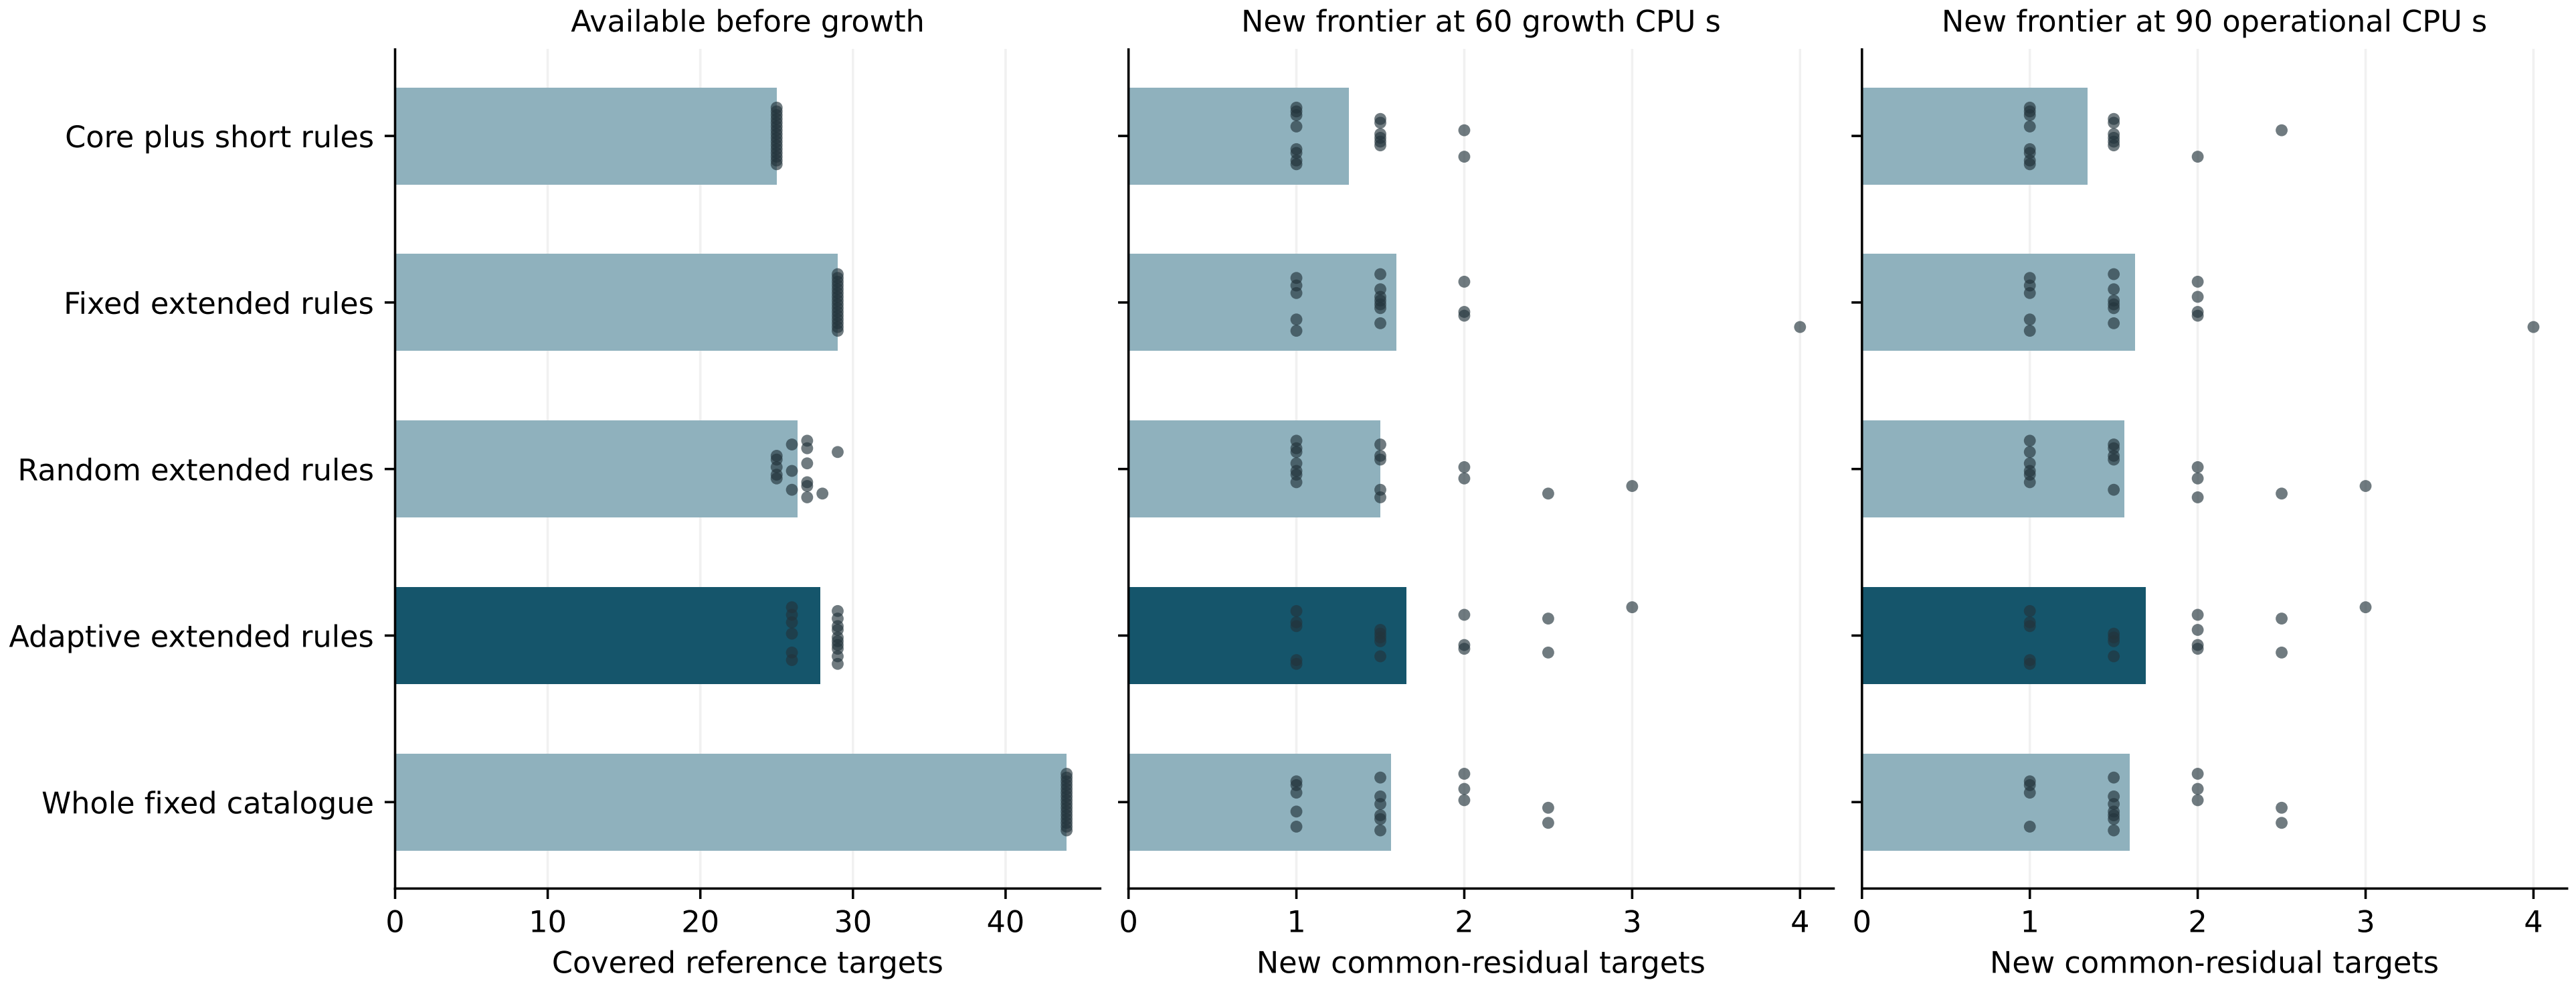
\includegraphics[width=\linewidth,height=.67\textheight,keepaspectratio]{Fig12.png}
\caption{Locked native comparison. Bars represent means over 16 source blocks; dots show source means after averaging the two neutral continuers. Initial coverage counts the whole reference, whereas the future panels count the common initial residual. The figure supplies descriptive variation, not confidence intervals}\label{fig:12}
\end{figure}

Evaluation receipt SHA-256: \path{e357a65de0f1cfe58b31e7de94c79d375946b6b47c2ca1f2a92963edda568d18}.

Independent review SHA-256: \path{29acbee7b2e5a7fec480985d8d8011123ee0da4e631656f858ed9bfe793f0931}.

Pipeline completion SHA-256: \path{97fff406c5e1e9ab2afb095756b91c39b675fc4b8b080ee01183c8792e471540}.

The complete registered report remains available in the frozen package, including all arms and paired outcomes. We neither retune on these targets nor infer equivalence from the failed superiority test. The fixed repertoire supplies the working configuration, not a post-hoc claim that it beats every alternative.

\section*{Appendix M. Extended historical comparisons}\label{appendix-m.-extended-historical-comparisons}
\addcontentsline{toc}{section}{Appendix M. Extended historical comparisons}

\subsection*{M.1. Reuse and the cost of the library}\label{m.1.-reuse-and-the-cost-of-the-library}
\addcontentsline{toc}{subsection}{M.1. Reuse and the cost of the library}

The passive library preserves the search path over common completed epochs. Across all 12 O--OB pairs, 3,503 paired checkpoints yield identical proof increments. At equal CPU time, however, OB changes the three means by \ensuremath{-}0.5\%, \ensuremath{-}1.1\%, and \ensuremath{-}2.4\%; small positive differences in some propositional pairs reflect costs, discrete layer boundaries, and runtime conditions. Such differences in finite prefixes do not reveal new search paths.

Subsequent proofs use the library frequently without establishing net savings for the full method. On eligible prefixes, OA records 35,777 direct later uses of library conclusions and OB records 47,246, each across twelve trajectories rather than that many independent observations. Later expanded proof terms shrink by approximately 82.6\% and 98.3\%, respectively, before charging the definitions again; the selector already charges them when it chooses the library, and the CPU budget includes the selector and the measurements. These gross savings concern expanded terms, not net pipeline cost, archive bytes, or search time.

A fragment can recur in new proofs without earning a scarce active slot. The passive library preserves its role in proofs without redirecting search, whereas the active library needs a separate rule for choosing premises. The present tests establish reuse but do not supply a universally effective rule for that choice.

\subsection*{M.2. How much of the human benchmark the method reaches}\label{m.2.-how-much-of-the-human-benchmark-the-method-reaches}
\addcontentsline{toc}{subsection}{M.2. How much of the human benchmark the method reaches}

The human comparison measures exact matches against 108 evaluation statements. The table reports means for the full archives at 60 CPU-seconds. These post-hoc counts describe human coverage rather than total formula novelty (Table 36).

\begingroup
\small
\setlength{\tabcolsep}{3pt}
\renewcommand{\arraystretch}{1.13}

\begin{longtable}[]{@{}
  >{\raggedright\arraybackslash}p{(\linewidth - 4\tabcolsep) * \real{0.3333}}
  >{\raggedleft\arraybackslash}p{(\linewidth - 4\tabcolsep) * \real{0.3333}}
  >{\raggedleft\arraybackslash}p{(\linewidth - 4\tabcolsep) * \real{0.3333}}@{}}
\caption{Mean exact human-reference matches in full archives at 60 CPU-seconds}\label{tab:36}\tabularnewline
\toprule\noalign{}
\begin{minipage}[b]{\linewidth}\raggedright
\textbf{Condition}
\end{minipage} & \begin{minipage}[b]{\linewidth}\raggedleft
\textbf{Prop.,} \(L = 25\)
\end{minipage} & \begin{minipage}[b]{\linewidth}\raggedleft
\textbf{Prop.,} \(L = 200\)
\end{minipage} \\
\midrule\noalign{}
\endfirsthead
\toprule\noalign{}
\begin{minipage}[b]{\linewidth}\raggedright
\textbf{Condition}
\end{minipage} & \begin{minipage}[b]{\linewidth}\raggedleft
\textbf{Prop.,} \(L = 25\)
\end{minipage} & \begin{minipage}[b]{\linewidth}\raggedleft
\textbf{Prop.,} \(L = 200\)
\end{minipage} \\
\midrule\noalign{}
\endhead
\bottomrule\noalign{}
\endlastfoot
P & 24 & 24 \\
O & 20.5 & 19 \\
OA & 20.75 & 19.25 \\
OB & 20.5 & 19 \\
\end{longtable}

\endgroup

The human endpoint ranks the methods differently from \(N_{60}\). We compared exact canonical formulae after the runs, starting from zero matches because no original axiom matches this benchmark. At \(L = 25\), O yields more formulae but fewer human matches, whereas OA gains only 0.25 matches over O at each size and does not close the gap to P. Neither final OA nor final OB library contains an exact match to the 108 statements, which says nothing about other potentially useful mathematical lemmas.

The active sets retain fewer human matches than the full archives. At the two sizes, their mean counts reach 13 and 12 for P, 4 and 5 for O, 3.25 and 5 for OA, and 3.75 and 4.75 for OB; P also keeps many more premises, so this contrast does not hold active-set size constant. Deactivation leaves each discovered human formula in the archive. Earlier experiments already used this benchmark, which neither represents all of Metamath nor supplies a full modal benchmark or an independent holdout.

\subsection*{M.3. What the earlier series contribute}\label{m.3.-what-the-earlier-series-contribute}
\addcontentsline{toc}{subsection}{M.3. What the earlier series contribute}

Earlier experiments explain the present architecture without contributing to a single pooled effect. Appendices C--G retain their full protocols, tables, and negative outcomes. The following table summarises how each series informed the current method while keeping their claims separate (Table 37).

\begingroup
\small
\setlength{\tabcolsep}{3pt}
\renewcommand{\arraystretch}{1.13}

\begin{longtable}[]{@{}
  >{\raggedright\arraybackslash}p{(\linewidth - 4\tabcolsep) * \real{0.2117}}
  >{\raggedright\arraybackslash}p{(\linewidth - 4\tabcolsep) * \real{0.4520}}
  >{\raggedright\arraybackslash}p{(\linewidth - 4\tabcolsep) * \real{0.3362}}@{}}
\caption{Separate contributions of earlier experimental series to the cumulative method}\label{tab:37}\tabularnewline
\toprule\noalign{}
\begin{minipage}[b]{\linewidth}\raggedright
\textbf{Series}
\end{minipage} & \begin{minipage}[b]{\linewidth}\raggedright
\textbf{Main result}
\end{minipage} & \begin{minipage}[b]{\linewidth}\raggedright
\textbf{Link to the present method}
\end{minipage} \\
\midrule\noalign{}
\endfirsthead
\toprule\noalign{}
\begin{minipage}[b]{\linewidth}\raggedright
\textbf{Series}
\end{minipage} & \begin{minipage}[b]{\linewidth}\raggedright
\textbf{Main result}
\end{minipage} & \begin{minipage}[b]{\linewidth}\raggedright
\textbf{Link to the present method}
\end{minipage} \\
\midrule\noalign{}
\endhead
\bottomrule\noalign{}
\endlastfoot
336 screening and 128 confirmatory trajectories & Queue policies and proof recipes helped some regimes but did not meet the overall advantage criterion & Motivates separate controls for active search and proof preservation \\
80 continuations from existing archives & Human-guided anchors yielded 1.94 and 1.64 times as many new schemata as random anchors at \(L = 25,200\); the axiom control found more new human matches & Shows conditional value in choosing anchors, not whether building the source pays off \\
96 context-transfer trajectories & The short-run advantage disappeared; at 180 CPU-seconds, means fell 14.8\% and 9.1\% below one-branch axiom growth at \(L = 25,200\) & Motivates removing the mandatory second branch and generator restart \\
\end{longtable}

\endgroup

The 80 continuations expose a limit of the automatic anchor criteria. All three static automatic criteria choose eight anchors, yet each yields fewer new formulae than the axiom control on every one of the 16 sources. Human-guided anchors improve on random anchors, but that result does not establish a fully automatic solution.

The series also differ in provenance and cost accounting. The confirmatory panel contains 124 original trajectories and four that we recovered after a local timer fix; the original incomplete audit remains available, and Appendices D and F document the deviation. The 80- and 96-trajectory series continue from earlier archives without charging their historical cost, whereas the new series starts from axioms. We cannot multiply these effects or treat them as a test of one jointly optimised pipeline.

\subsection*{M.4. Prospective leases on new scheduler states}\label{m.4.-prospective-leases-on-new-scheduler-states}
\addcontentsline{toc}{subsection}{M.4. Prospective leases on new scheduler states}

A separate series compares four policies on states 7401--7404 with the same controller parameters as the pilot. Nested readings occur at 10 and 30 CPU-seconds. The following table reports mean certified new-formula counts at 30 seconds. OA6 uses fixed leases without renewal, so its results do not join the historical OA sample (Table 38).

\begingroup
\small
\setlength{\tabcolsep}{3pt}
\renewcommand{\arraystretch}{1.13}

\begin{longtable}[]{@{}
  >{\raggedright\arraybackslash}p{(\linewidth - 8\tabcolsep) * \real{0.2000}}
  >{\raggedleft\arraybackslash}p{(\linewidth - 8\tabcolsep) * \real{0.2000}}
  >{\raggedleft\arraybackslash}p{(\linewidth - 8\tabcolsep) * \real{0.2000}}
  >{\raggedleft\arraybackslash}p{(\linewidth - 8\tabcolsep) * \real{0.2000}}
  >{\raggedleft\arraybackslash}p{(\linewidth - 8\tabcolsep) * \real{0.2000}}@{}}
\caption{Mean new-formula counts for prospective policies at 30 CPU-seconds on new states}\label{tab:38}\tabularnewline
\toprule\noalign{}
\begin{minipage}[b]{\linewidth}\raggedright
\textbf{Stratum}
\end{minipage} & \begin{minipage}[b]{\linewidth}\raggedleft
\textbf{OB}
\end{minipage} & \begin{minipage}[b]{\linewidth}\raggedleft
\textbf{OA6}
\end{minipage} & \begin{minipage}[b]{\linewidth}\raggedleft
\textbf{OP}
\end{minipage} & \begin{minipage}[b]{\linewidth}\raggedleft
\textbf{OL}
\end{minipage} \\
\midrule\noalign{}
\endfirsthead
\toprule\noalign{}
\begin{minipage}[b]{\linewidth}\raggedright
\textbf{Stratum}
\end{minipage} & \begin{minipage}[b]{\linewidth}\raggedleft
\textbf{OB}
\end{minipage} & \begin{minipage}[b]{\linewidth}\raggedleft
\textbf{OA6}
\end{minipage} & \begin{minipage}[b]{\linewidth}\raggedleft
\textbf{OP}
\end{minipage} & \begin{minipage}[b]{\linewidth}\raggedleft
\textbf{OL}
\end{minipage} \\
\midrule\noalign{}
\endhead
\bottomrule\noalign{}
\endlastfoot
Prop., \(L = 25\) & 52,606.5 & 62,849.25 & 61,328.25 & 61,536.75 \\
Prop., \(L = 200\) & 80,635.25 & 75,869 & 80,105.75 & 71,800.75 \\
Modal K, \(L = 25\) & 54,706.5 & 71,432.5 & 60,533.5 & 60,649 \\
\end{longtable}

\endgroup

Ratios of means give the following gains relative to OB: propositional \(L = 25\): OP +16.6\% with 3/4 positive pairs, and OL +17.0\% with 2/4; propositional \(L = 200\): OP -0.7\% with 3/4 positive pairs, and OL -11.0\% with 1/4; modal K \(L = 25\): OP +10.7\% with 4/4 positive pairs, and OL +10.9\% with 3/4.

Both prospective policies exceed the passive library in mean formula output in the two size-25 strata at 30 seconds. OP improves all four modal pairs, but only three of four propositional pairs; OL improves three and two pairs, respectively. These outcomes describe the tested scheduler states, not a uniform or statistically established advantage. Appendix H reports every pair and the ten-second outcomes (Fig. 13).

\begin{figure}[!htbp]
\centering
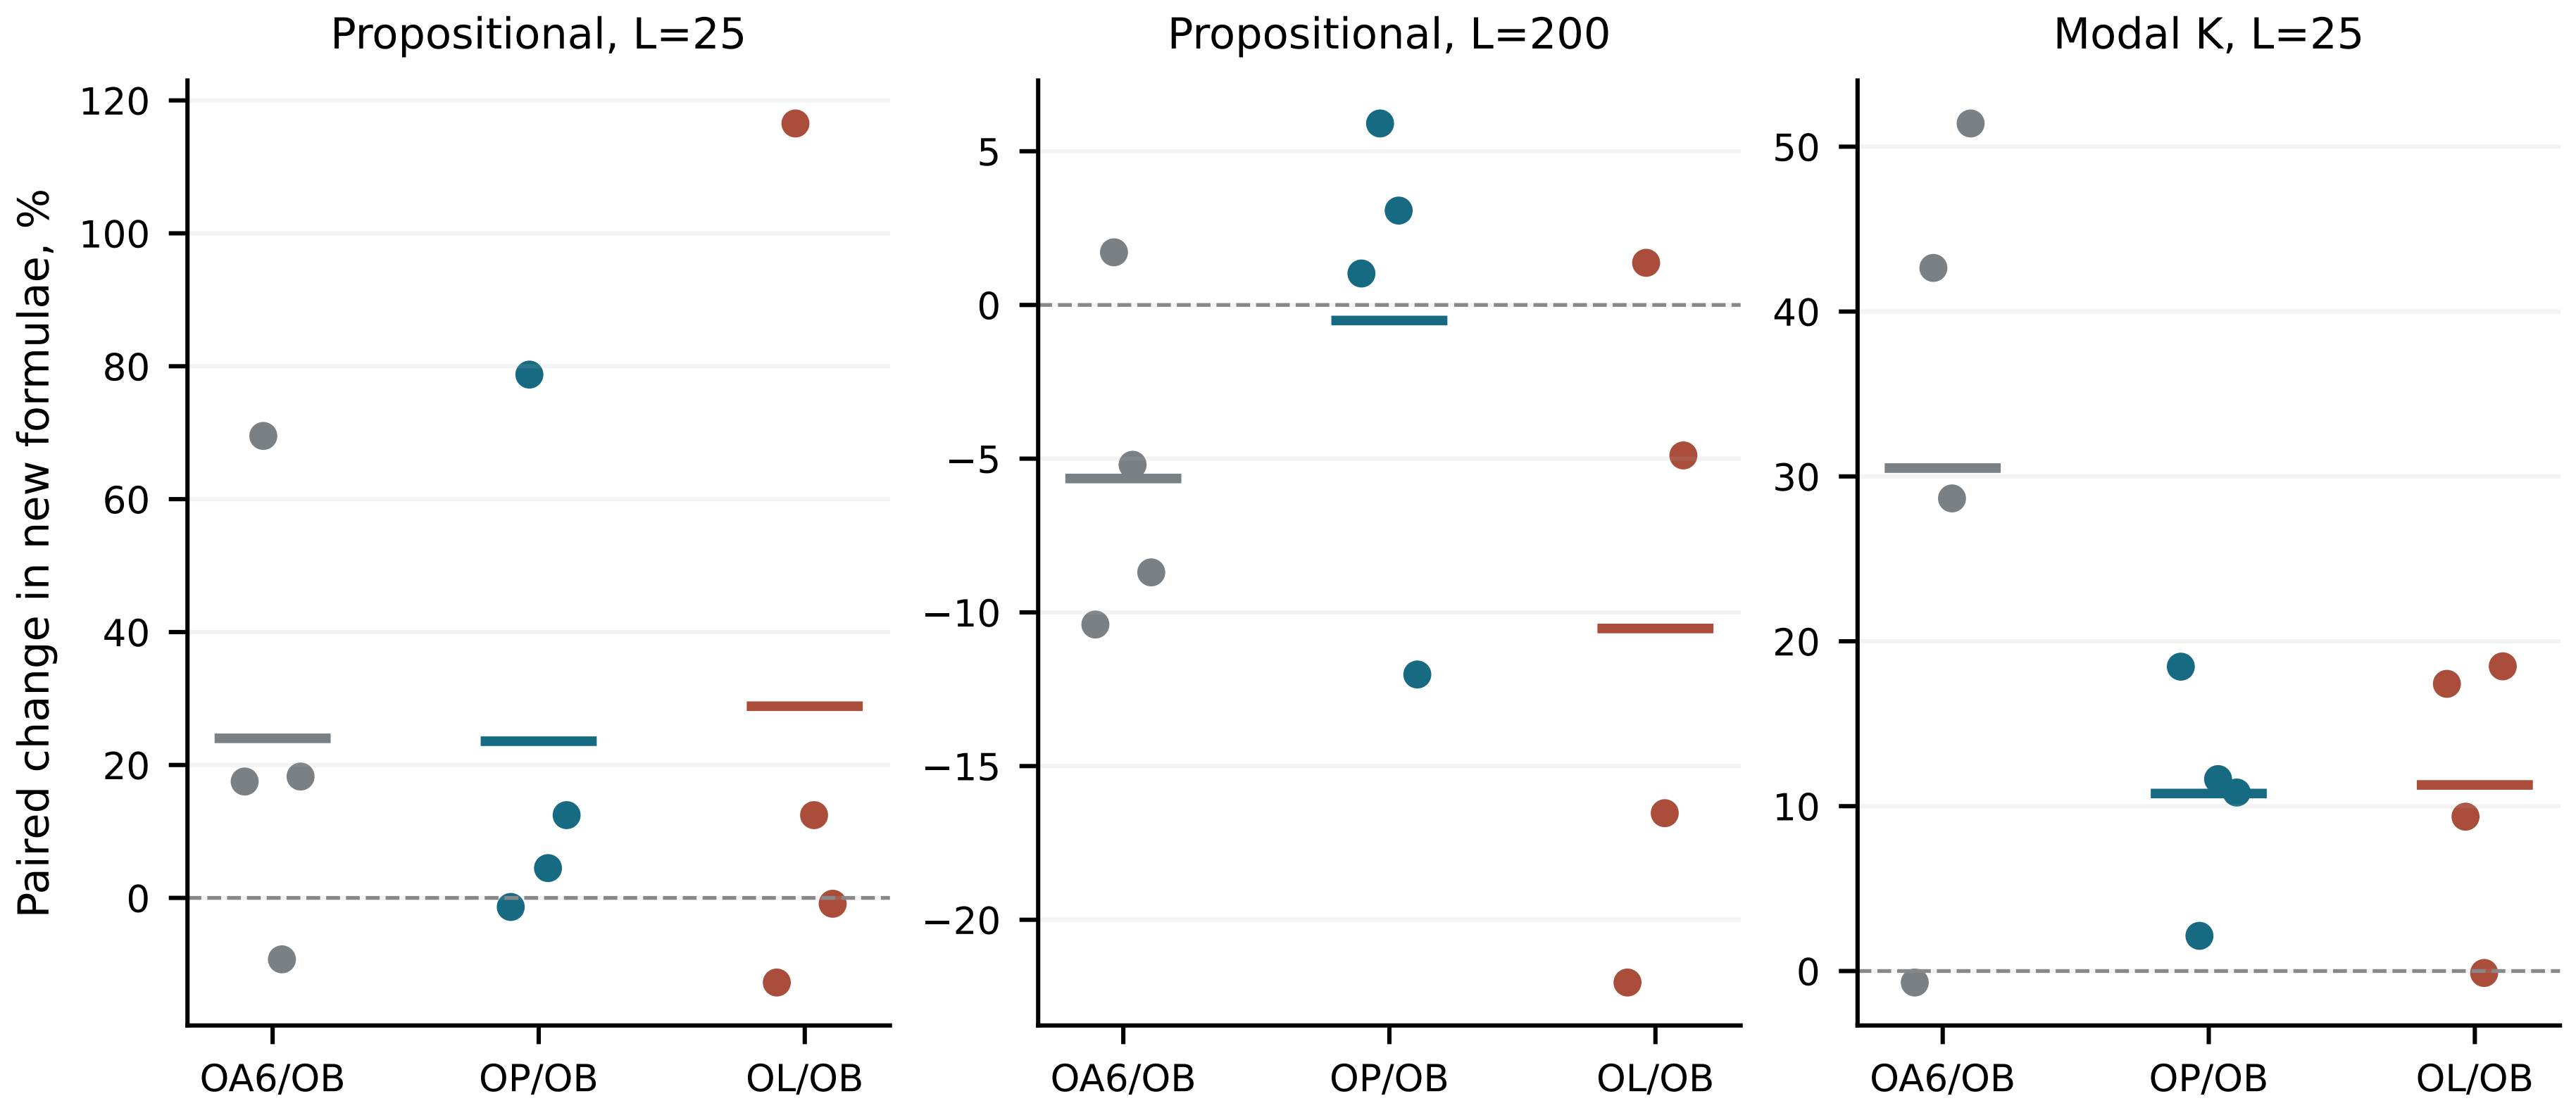
\includegraphics[width=\linewidth,height=.67\textheight,keepaspectratio]{Fig13.png}
\caption{Paired changes relative to the passive library at 30 CPU-seconds. Points denote four scheduler states; short horizontal segments mark mean paired changes rather than confidence intervals. Mean paired changes may differ from gains from ratios of means in the text}\label{fig:13}
\end{figure}

The comparison identifies a regime-dependent trade-off between simple leasing and prospective choice. OA6 yields more formulae on average than OP or OL in both size-25 strata. In those two strata, prospective policy work consumes about 1.14--1.39 CPU-seconds, versus 0.78--0.83 for OA6, including more than the probes alone. At propositional size 200, OP exceeds OA6 by 5.6\% from the ratio of means; its mean falls 0.7\% below OB, versus 5.9\% for OA6. These results favour prospective choice over unconditional leases at that size and leave the causes of the contrast to a separate feature-level experiment.

A post-hoc check against the previous 108 Metamath statements ranks the policies differently. At propositional size 25, OP reaches a mean of 21.5 exact archive matches, versus 19.25 for OB, 20 for OA6, and 19 for OL. Its active set retains a mean of five matches, tying OL and exceeding OA6 at 4.5 and OB at 2.75. These counts concern statements, not similarity between proofs, and reuse an earlier benchmark rather than an independent holdout. They do not change the primary policy criterion; Section H.6 reports the remaining results and limits.

\section*{Appendix N. Cumulative skeleton networks}\label{appendix-n.-cumulative-skeleton-networks}
\addcontentsline{toc}{section}{Appendix N. Cumulative skeleton networks}

\subsection*{N.1. Projections and representative choice}\label{n.1.-projections-and-representative-choice}
\addcontentsline{toc}{subsection}{N.1. Projections and representative choice}

The new descriptive study reads only audited initial libraries from the corrected holdout. Each projection includes every available anchor, all 29 basis roots, and every necessary certificate ancestor. The projection joins each parent to the conclusion and collapses duplicate arcs. Hidden ancestors retain proof roles but no automatic search rights. The first source, 2026102201, supplies both representatives. The main text uses its fixed quota-matched control because adaptive ranking failed the registered rule; the image below retains the adaptive representative that we chose before scoring. This editorial fallback does not relabel adaptive as an effective method or select the highest-performing control.

Panels a, c, and d retain their old graph hashes and layouts. Panels c and d also retain their shared coordinates, colours, and vertex areas. Panel b uses the same fixed layout seed, three-start community search, and vertex-area rule. All vertices and unique undirected edges enter every drawing. Layout distances across independently scaled panels do not measure comparable semantic proximity (Fig. 14).

\begin{figure}[!htbp]
\centering
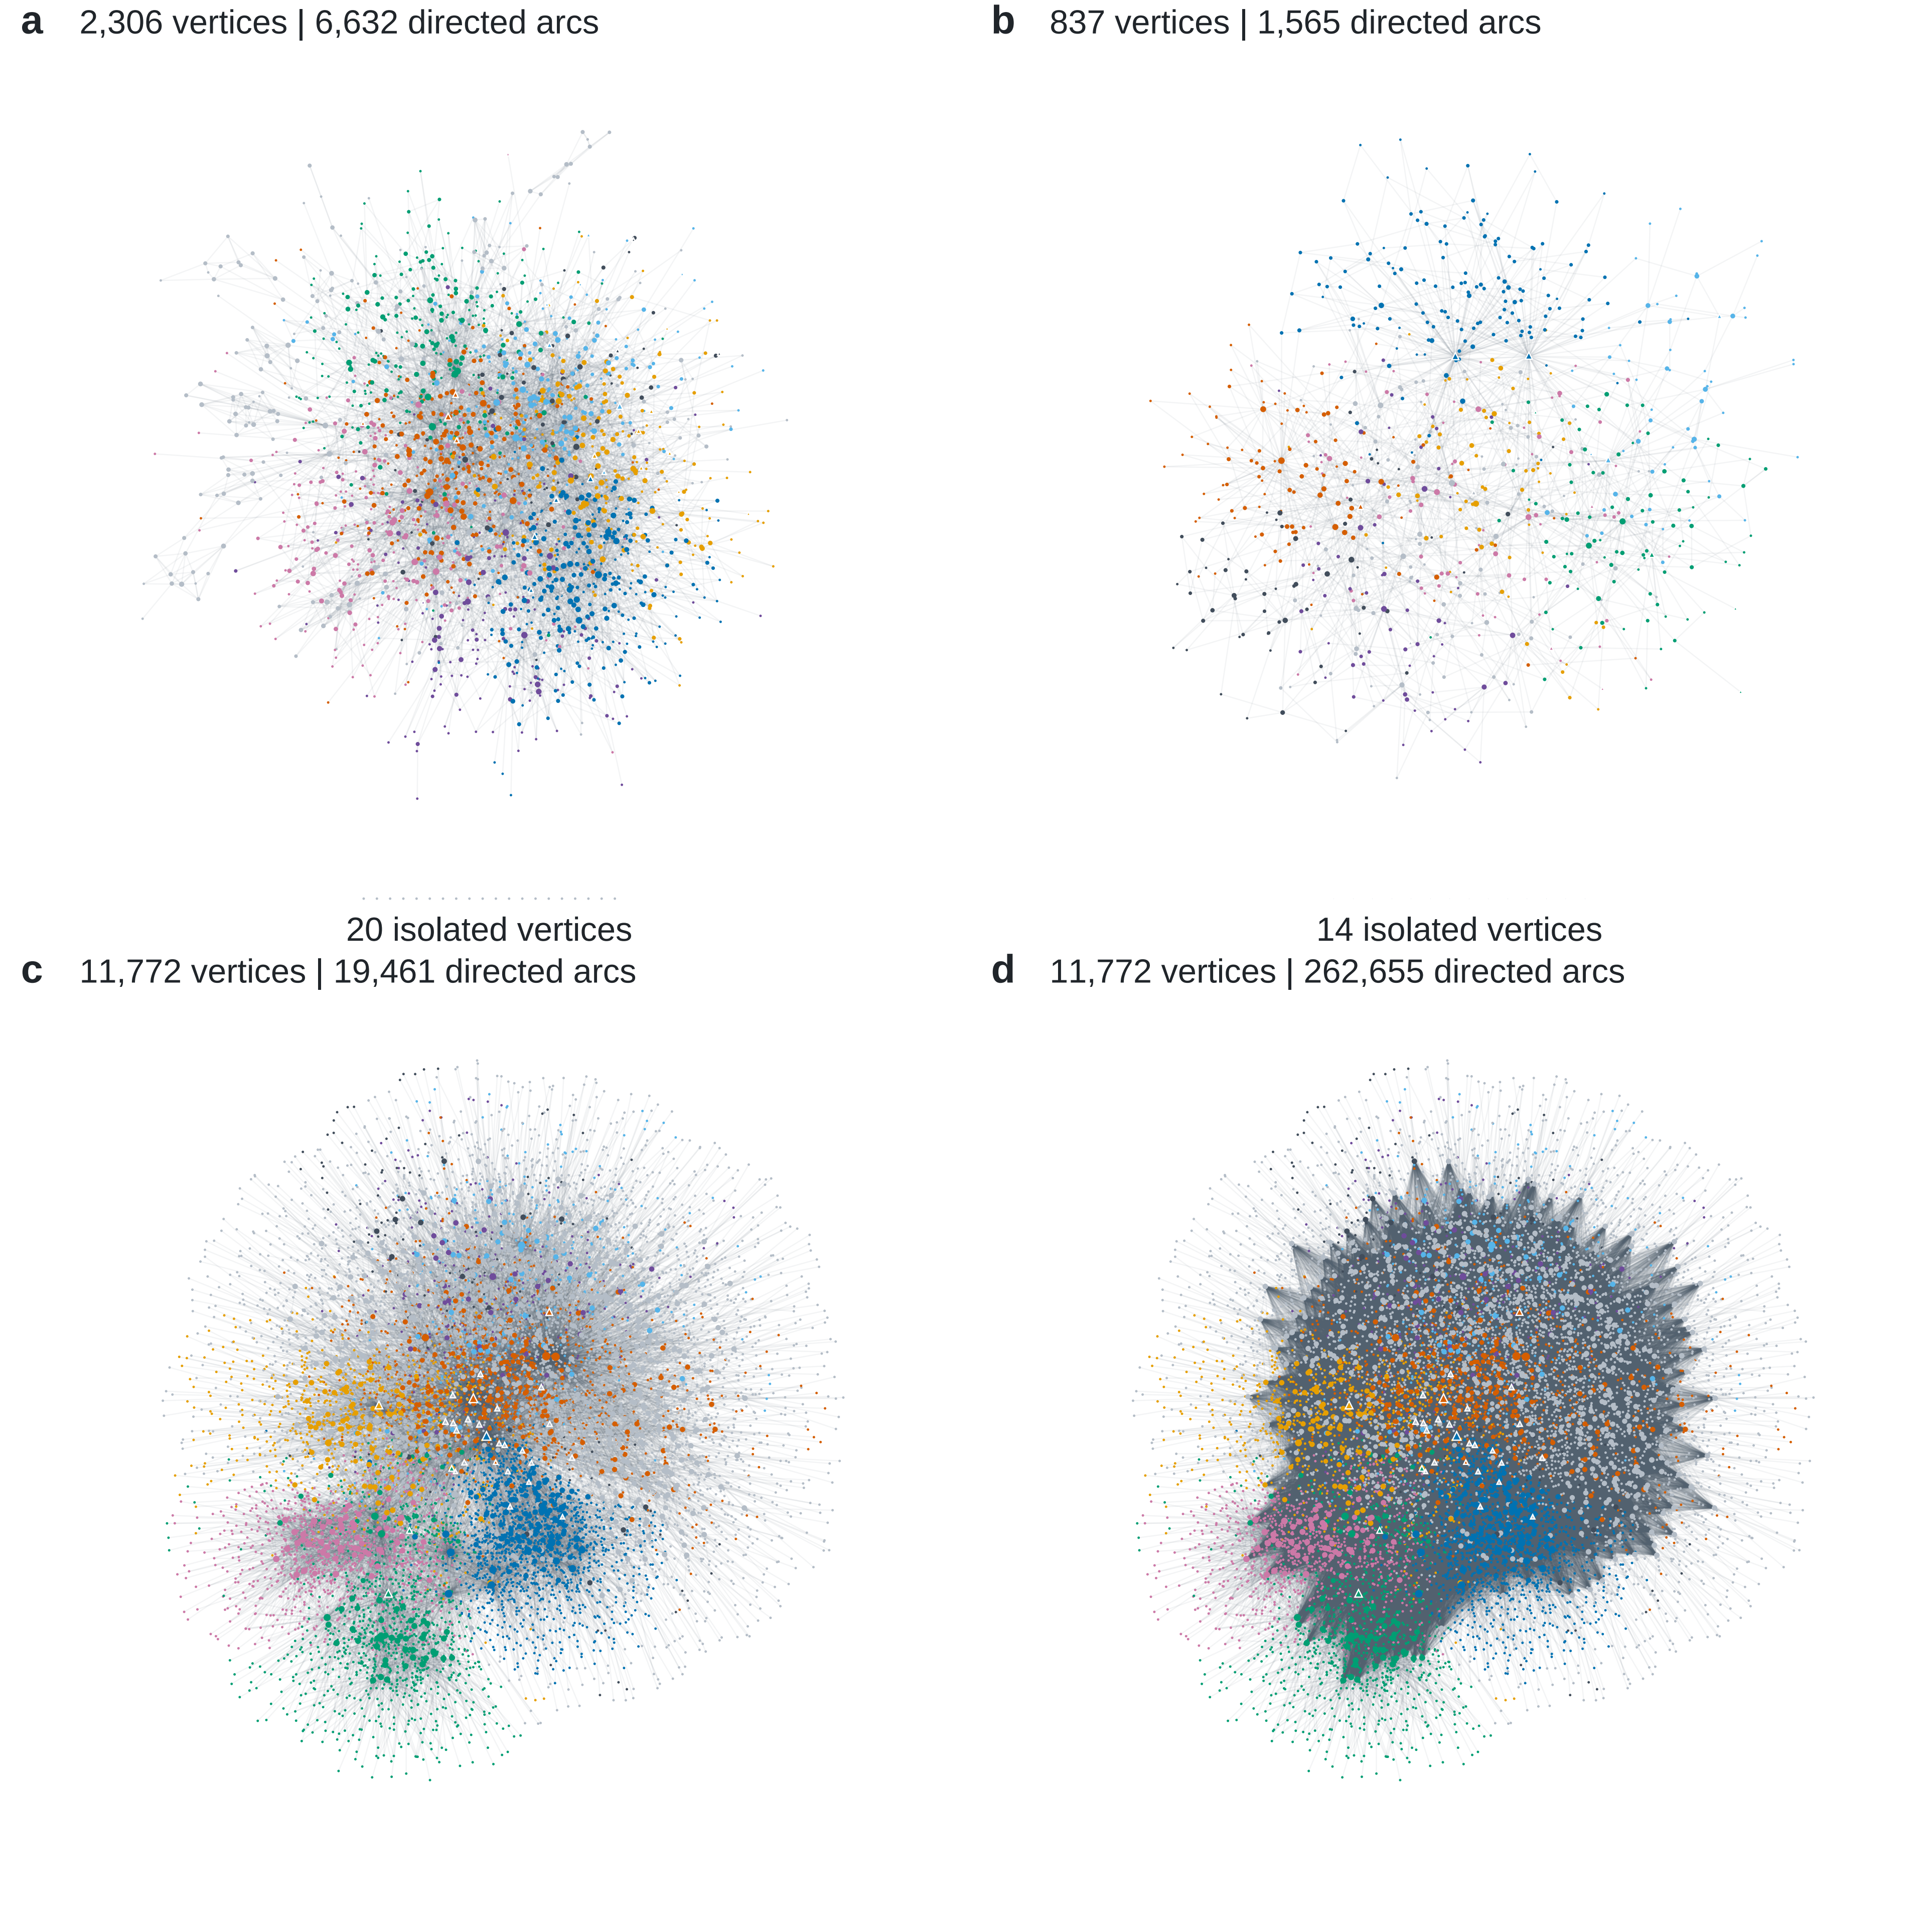
\includegraphics[width=\linewidth,height=.67\textheight,keepaspectratio]{Fig14.png}
\caption{Preselected adaptive test variant on the same basis. Panel b uses adaptive initial source 2026102201, not the best continuation or target-coverage result. The remaining panels retain the frozen Metamath and height-three graphs and layouts. This graph illustrates a tested variant without an established adaptive advantage}\label{fig:14}
\end{figure}

\subsection*{N.2. Profiles across all source states}\label{n.2.-profiles-across-all-source-states}
\addcontentsline{toc}{subsection}{N.2. Profiles across all source states}

Every source contributes one initial library for each of the two reported methods, not two independent theories. Anchors exclude basis roots; certificate vertices include roots and hidden support. C denotes mean local clustering, L the exact mean path on the largest undirected component, Q the best modularity across three Louvain starts, and Q0 the mean over ten simple degree-preserving null graphs. Every new observed and null graph uses all BFS sources.

\subsubsection*{Fixed repertoire}\label{fixed-repertoire}
\addcontentsline{toc}{subsubsection}{Fixed repertoire}

Table 39 reports each fixed-repertoire initial skeleton; source suffixes follow the frozen order.

\begingroup
\small
\setlength{\tabcolsep}{3pt}
\renewcommand{\arraystretch}{1.13}

\begin{longtable}[]{@{}
  >{\raggedright\arraybackslash}p{(\linewidth - 14\tabcolsep) * \real{0.1238}}
  >{\raggedleft\arraybackslash}p{(\linewidth - 14\tabcolsep) * \real{0.1172}}
  >{\raggedleft\arraybackslash}p{(\linewidth - 14\tabcolsep) * \real{0.1732}}
  >{\raggedleft\arraybackslash}p{(\linewidth - 14\tabcolsep) * \real{0.1172}}
  >{\raggedleft\arraybackslash}p{(\linewidth - 14\tabcolsep) * \real{0.1172}}
  >{\raggedleft\arraybackslash}p{(\linewidth - 14\tabcolsep) * \real{0.1172}}
  >{\raggedleft\arraybackslash}p{(\linewidth - 14\tabcolsep) * \real{0.1172}}
  >{\raggedleft\arraybackslash}p{(\linewidth - 14\tabcolsep) * \real{0.1172}}@{}}
\caption{Network profiles of all 16 fixed-repertoire initial skeletons}\label{tab:39}\tabularnewline
\toprule\noalign{}
\begin{minipage}[b]{\linewidth}\raggedright
\textbf{Source suffix}
\end{minipage} & \begin{minipage}[b]{\linewidth}\raggedleft
\textbf{Anchors}
\end{minipage} & \begin{minipage}[b]{\linewidth}\raggedleft
\textbf{Certificate vertices}
\end{minipage} & \begin{minipage}[b]{\linewidth}\raggedleft
\textbf{Arcs}
\end{minipage} & \begin{minipage}[b]{\linewidth}\raggedleft
\textbf{C}
\end{minipage} & \begin{minipage}[b]{\linewidth}\raggedleft
\textbf{L}
\end{minipage} & \begin{minipage}[b]{\linewidth}\raggedleft
\textbf{Q}
\end{minipage} & \begin{minipage}[b]{\linewidth}\raggedleft
\textbf{Q0}
\end{minipage} \\
\midrule\noalign{}
\endfirsthead
\toprule\noalign{}
\begin{minipage}[b]{\linewidth}\raggedright
\textbf{Source suffix}
\end{minipage} & \begin{minipage}[b]{\linewidth}\raggedleft
\textbf{Anchors}
\end{minipage} & \begin{minipage}[b]{\linewidth}\raggedleft
\textbf{Certificate vertices}
\end{minipage} & \begin{minipage}[b]{\linewidth}\raggedleft
\textbf{Arcs}
\end{minipage} & \begin{minipage}[b]{\linewidth}\raggedleft
\textbf{C}
\end{minipage} & \begin{minipage}[b]{\linewidth}\raggedleft
\textbf{L}
\end{minipage} & \begin{minipage}[b]{\linewidth}\raggedleft
\textbf{Q}
\end{minipage} & \begin{minipage}[b]{\linewidth}\raggedleft
\textbf{Q0}
\end{minipage} \\
\midrule\noalign{}
\endhead
\bottomrule\noalign{}
\endlastfoot
01 & 675 & 841 & 1573 & 0.0202 & 4.177 & 0.622 & 0.539 \\
02 & 679 & 852 & 1594 & 0.0199 & 4.179 & 0.622 & 0.542 \\
03 & 665 & 836 & 1564 & 0.0189 & 4.175 & 0.623 & 0.541 \\
04 & 669 & 840 & 1572 & 0.0200 & 4.175 & 0.624 & 0.541 \\
05 & 679 & 847 & 1585 & 0.0200 & 4.167 & 0.623 & 0.541 \\
06 & 669 & 840 & 1571 & 0.0199 & 4.171 & 0.622 & 0.543 \\
07 & 682 & 848 & 1586 & 0.0186 & 4.169 & 0.628 & 0.541 \\
08 & 672 & 844 & 1578 & 0.0207 & 4.179 & 0.623 & 0.541 \\
09 & 674 & 845 & 1583 & 0.0215 & 4.181 & 0.624 & 0.541 \\
10 & 677 & 849 & 1587 & 0.0207 & 4.177 & 0.629 & 0.541 \\
11 & 669 & 840 & 1571 & 0.0188 & 4.183 & 0.625 & 0.540 \\
12 & 674 & 848 & 1589 & 0.0203 & 4.180 & 0.628 & 0.541 \\
13 & 681 & 848 & 1586 & 0.0186 & 4.189 & 0.625 & 0.544 \\
14 & 681 & 849 & 1588 & 0.0207 & 4.165 & 0.624 & 0.540 \\
15 & 672 & 844 & 1579 & 0.0204 & 4.175 & 0.629 & 0.539 \\
16 & 682 & 851 & 1594 & 0.0201 & 4.171 & 0.624 & 0.542 \\
\end{longtable}

\endgroup

Mean anchors: 675.0000; mean certificate vertices: 845.1250; mean modularity: 0.6246.

\subsubsection*{Adaptive test variant}\label{adaptive-test-variant}
\addcontentsline{toc}{subsubsection}{Adaptive test variant}

Table 40 reports the adaptive-test initial skeletons in the same source order.

\begingroup
\small
\setlength{\tabcolsep}{3pt}
\renewcommand{\arraystretch}{1.13}

\begin{longtable}[]{@{}
  >{\raggedright\arraybackslash}p{(\linewidth - 14\tabcolsep) * \real{0.1238}}
  >{\raggedleft\arraybackslash}p{(\linewidth - 14\tabcolsep) * \real{0.1172}}
  >{\raggedleft\arraybackslash}p{(\linewidth - 14\tabcolsep) * \real{0.1732}}
  >{\raggedleft\arraybackslash}p{(\linewidth - 14\tabcolsep) * \real{0.1172}}
  >{\raggedleft\arraybackslash}p{(\linewidth - 14\tabcolsep) * \real{0.1172}}
  >{\raggedleft\arraybackslash}p{(\linewidth - 14\tabcolsep) * \real{0.1172}}
  >{\raggedleft\arraybackslash}p{(\linewidth - 14\tabcolsep) * \real{0.1172}}
  >{\raggedleft\arraybackslash}p{(\linewidth - 14\tabcolsep) * \real{0.1172}}@{}}
\caption{Network profiles of all 16 adaptive-test initial skeletons}\label{tab:40}\tabularnewline
\toprule\noalign{}
\begin{minipage}[b]{\linewidth}\raggedright
\textbf{Source suffix}
\end{minipage} & \begin{minipage}[b]{\linewidth}\raggedleft
\textbf{Anchors}
\end{minipage} & \begin{minipage}[b]{\linewidth}\raggedleft
\textbf{Certificate vertices}
\end{minipage} & \begin{minipage}[b]{\linewidth}\raggedleft
\textbf{Arcs}
\end{minipage} & \begin{minipage}[b]{\linewidth}\raggedleft
\textbf{C}
\end{minipage} & \begin{minipage}[b]{\linewidth}\raggedleft
\textbf{L}
\end{minipage} & \begin{minipage}[b]{\linewidth}\raggedleft
\textbf{Q}
\end{minipage} & \begin{minipage}[b]{\linewidth}\raggedleft
\textbf{Q0}
\end{minipage} \\
\midrule\noalign{}
\endfirsthead
\toprule\noalign{}
\begin{minipage}[b]{\linewidth}\raggedright
\textbf{Source suffix}
\end{minipage} & \begin{minipage}[b]{\linewidth}\raggedleft
\textbf{Anchors}
\end{minipage} & \begin{minipage}[b]{\linewidth}\raggedleft
\textbf{Certificate vertices}
\end{minipage} & \begin{minipage}[b]{\linewidth}\raggedleft
\textbf{Arcs}
\end{minipage} & \begin{minipage}[b]{\linewidth}\raggedleft
\textbf{C}
\end{minipage} & \begin{minipage}[b]{\linewidth}\raggedleft
\textbf{L}
\end{minipage} & \begin{minipage}[b]{\linewidth}\raggedleft
\textbf{Q}
\end{minipage} & \begin{minipage}[b]{\linewidth}\raggedleft
\textbf{Q0}
\end{minipage} \\
\midrule\noalign{}
\endhead
\bottomrule\noalign{}
\endlastfoot
01 & 668 & 837 & 1565 & 0.0197 & 4.170 & 0.631 & 0.541 \\
02 & 679 & 852 & 1594 & 0.0199 & 4.179 & 0.622 & 0.542 \\
03 & 662 & 832 & 1556 & 0.0184 & 4.169 & 0.626 & 0.542 \\
04 & 673 & 843 & 1578 & 0.0185 & 4.160 & 0.624 & 0.541 \\
05 & 672 & 843 & 1577 & 0.0195 & 4.161 & 0.626 & 0.542 \\
06 & 669 & 840 & 1571 & 0.0199 & 4.171 & 0.622 & 0.543 \\
07 & 682 & 848 & 1586 & 0.0186 & 4.169 & 0.628 & 0.541 \\
08 & 669 & 840 & 1570 & 0.0202 & 4.173 & 0.619 & 0.541 \\
09 & 674 & 845 & 1583 & 0.0215 & 4.181 & 0.624 & 0.541 \\
10 & 677 & 849 & 1587 & 0.0207 & 4.177 & 0.629 & 0.541 \\
11 & 669 & 840 & 1571 & 0.0188 & 4.183 & 0.625 & 0.540 \\
12 & 674 & 848 & 1589 & 0.0203 & 4.180 & 0.628 & 0.541 \\
13 & 675 & 846 & 1583 & 0.0181 & 4.182 & 0.619 & 0.542 \\
14 & 681 & 849 & 1588 & 0.0207 & 4.165 & 0.624 & 0.540 \\
15 & 669 & 840 & 1571 & 0.0199 & 4.169 & 0.617 & 0.540 \\
16 & 682 & 851 & 1594 & 0.0201 & 4.171 & 0.624 & 0.542 \\
\end{longtable}

\endgroup

Mean anchors: 673.4375; mean certificate vertices: 843.9375; mean modularity: 0.6243.

\subsection*{N.3. Tail diagnostics and reproducibility}\label{n.3.-tail-diagnostics-and-reproducibility}
\addcontentsline{toc}{subsection}{N.3. Tail diagnostics and reproducibility}

For each outgoing distinct-use profile, the diagnostic uses 20,000 bootstrap draws for the exact discrete pure power-law family and refits the threshold and exponent in every draw. The earlier in-degree and undirected-degree alternatives remain secondary descriptions. Conditional tail diagnostics do not assume independent graph replicates or establish a limiting law. Small-world ratios compare clustering and largest-component paths with ten degree-preserving controls, not a universal classifier.

Across all 16 fixed sources, pure-family bootstrap p-values range from 0.24190 to 0.62575; across the 16 adaptive variants, they range from 0.17950 to 0.62575. None rejects that family at five percent. The new certificate projections retain 13--15 isolated unused basis roots, which still enter the vertex count and zero-degree mass; both illustrated representatives contain 14. A compatible finite tail neither confirms adaptive future-use superiority nor proves that the generator intrinsically converges to a scale-free network. The machine-readable profiles retain thresholds, exponents, binomial Monte Carlo intervals, zero-degree counts, and same-tail alternative likelihoods for every source.

The package \path{output/article1_adaptive_revision_20261021_v1/networks/} retains graph arrays, original checkpoint hashes, per-source structural and tail profiles, all null records, representative coordinates, figures, and the drawing audit. The old study in Appendix J remains a distinct historical stage; none of its skeleton counts substitutes for the new panel b. The editorial scientific gate separately verifies all blind receipts and evaluation-file hashes before this descriptive analysis.

\clearpage
\section*{Statements and Declarations}

\subsection*{Data availability}\label{data-availability}
\addcontentsline{toc}{subsection}{Data availability}

We publicly provide source code for the main native workflow, self-contained tests, and compact checked results at https://github.com/nnevdokimov/certified-proof-skeleton. Frozen packages and the editorial manifest identify the protocols, code versions, input hashes, and numerical sources. We do not yet provide the complete experimental record in a permanent archive. The source release does not include a reuse licence; third-party inputs retain their original licence requirements.

\subsection*{Conflicts of interest}\label{conflicts-of-interest}
\addcontentsline{toc}{subsection}{Conflicts of interest}

The authors declare no conflict of interest concerning this article.

\subsection*{Funding}\label{funding}
\addcontentsline{toc}{subsection}{Funding}

The research leading to these results received funding from the Basic Research Program at HSE University {[}HSE-BR-2025-025{]}.

\subsection*{Acknowledgments}\label{acknowledgments}
\addcontentsline{toc}{subsection}{Acknowledgments}

We used the HSE University supercomputer to conduct the computational research.

\begin{thebibliography}{37}
\bibitem{MetamathSetMMPinned} Metamath Project. (2026). \emph{set.mm: ZFC set theory database, fixed experimental version}. \url{https://github.com/metamath/set.mm/commit/584b6852f57f281e9be1793332f1e52e077693c8}

\bibitem{BachmairGanzinger2001} Bachmair, L., \& Ganzinger, H. (2001). Resolution theorem proving. In J. A. Robinson \& A. Voronkov (Eds.), \emph{Handbook of automated reasoning} (pp. 19--99). Elsevier. \url{https://doi.org/10.1016/B978-044450813-3/50004-7}

\bibitem{Wernhard2026} Wernhard, C. (2026). Generating theorems by generating proof structures. \emph{Automated Reasoning: IJCAR 2026, Lecture Notes in Computer Science}, \emph{16688}, 41--61. \url{https://doi.org/10.1007/978-3-032-32589-1_3}

\bibitem{Schulz2002} Schulz, S. (2002). E -- a brainiac theorem prover. \emph{AI Communications}, \emph{15}(2--3), 111--126. \url{https://doi.org/10.3233/EAI-2002-260}

\bibitem{KovacsVoronkov2013} Kov\'{a}cs, L., \& Voronkov, A. (2013). First-order theorem proving and Vampire. \emph{Computer Aided Verification}, 1--35. \url{https://doi.org/10.1007/978-3-642-39799-8_1}

\bibitem{RiazanovVoronkov2003LRS} Riazanov, A., \& Voronkov, A. (2003). Limited resource strategy in resolution theorem proving. \emph{Journal of Symbolic Computation}, \emph{36}(1--2), 101--115. \url{https://doi.org/10.1016/S0747-7171(03)00040-3}

\bibitem{HoderVoronkov2011} Hoder, K., \& Voronkov, A. (2011). Sine qua non for large theory reasoning. \emph{Automated Deduction -- CADE-23}, 299--314. \url{https://doi.org/10.1007/978-3-642-22438-6_23}

\bibitem{BlanchetteEtAl2016} Blanchette, J. C., Greenaway, D., Kaliszyk, C., K\"{u}hlwein, D., \& Urban, J. (2016). A learning-based fact selector for Isabelle/HOL. \emph{Journal of Automated Reasoning}, \emph{57}(3), 219--244. \url{https://doi.org/10.1007/s10817-016-9362-8}

\bibitem{JakubuvUrban2017} Jakub\r{u}v, J., \& Urban, J. (2017). ENIGMA: Efficient learning-based inference guiding machine. \emph{Intelligent Computer Mathematics}, 292--302. \url{https://doi.org/10.1007/978-3-319-62075-6_20}

\bibitem{Colton2002} Colton, S. (2002). \emph{Automated theory formation in pure mathematics}. Springer. \url{https://doi.org/10.1007/978-1-4471-0147-5}

\bibitem{SmallboneEtAl2017} Smallbone, N., Johansson, M., Claessen, K., \& Algehed, M. (2017). Quick specifications for the busy programmer. \emph{Journal of Functional Programming}, \emph{27}, e18. \url{https://doi.org/10.1017/S0956796817000090}

\bibitem{ClaessenEtAl2013} Claessen, K., Johansson, M., Ros\'{e}n, D., \& Smallbone, N. (2013). Automating inductive proofs using theory exploration. \emph{Automated Deduction -- CADE-24, Lecture Notes in Computer Science}, \emph{7898}, 392--406. \url{https://doi.org/10.1007/978-3-642-38574-2_27}

\bibitem{JohanssonEtAl2014} Johansson, M., Ros\'{e}n, D., Smallbone, N., \& Claessen, K. (2014). Hipster: Integrating theory exploration in a proof assistant. \emph{Intelligent Computer Mathematics}, 108--122. \url{https://doi.org/10.1007/978-3-319-08434-3_9}

\bibitem{SingherItzhaky2021} Singher, E., \& Itzhaky, S. (2021). Theory exploration powered by deductive synthesis. \emph{Computer Aided Verification, Lecture Notes in Computer Science}, \emph{12760}, 125--148. \url{https://doi.org/10.1007/978-3-030-81688-9_6}

\bibitem{McCaslandBundySmith2017} McCasland, R. L., Bundy, A., \& Smith, P. F. (2017). MATHsAiD: Automated mathematical theory exploration. \emph{Applied Intelligence, 47}, 585--606. \url{https://doi.org/10.1007/s10489-017-0954-8}

\bibitem{WernhardBibel2024} Wernhard, C., \& Bibel, W. (2024). Investigations into proof structures. \emph{Journal of Automated Reasoning}, \emph{68}, 24. \url{https://doi.org/10.1007/s10817-024-09711-8}

\bibitem{RawsonEtAl2023} Rawson, M., Wernhard, C., Zombori, Z., \& Bibel, W. (2023). Lemmas: Generation, selection, application. \emph{Automated Reasoning with Analytic Tableaux and Related Methods}, 153--174. \url{https://doi.org/10.1007/978-3-031-43513-3_9}

\bibitem{WernhardZombori2025} Wernhard, C., \& Zombori, Z. (2025). Mathematical knowledge bases as grammar-compressed proof terms: Exploring Metamath proof structures. \emph{arXiv Preprint arXiv:2505.12305}. \url{https://doi.org/10.48550/arXiv.2505.12305}

\bibitem{Minton1990Utility} Minton, S. (1990). Quantitative results concerning the utility of explanation-based learning. \emph{Artificial Intelligence}, \emph{42}(2--3), 363--391. \url{https://doi.org/10.1016/0004-3702(90)90059-9}

\bibitem{KaliszykUrban2015} Kaliszyk, C., \& Urban, J. (2015). Learning-assisted theorem proving with millions of lemmas. \emph{Journal of Symbolic Computation}, \emph{69}, 109--128. \url{https://doi.org/10.1016/j.jsc.2014.09.032}

\bibitem{WangEtAl2023Lego} Wang, H., Xin, H., Zheng, C., Liu, Z., Cao, Q., Huang, Y., Xiong, J., Shi, H., Xie, E., Yin, J., Li, Z., \& Liang, X. (2024). LEGO-Prover: Neural theorem proving with growing libraries. \emph{The Twelfth International Conference on Learning Representations}. \url{https://proceedings.iclr.cc/paper_files/paper/2024/hash/85dca46374dc0f27b4bb5f265b3d17f0-Abstract-Conference.html}

\bibitem{YangEtAl2023} Yang, K., Swope, A., Gu, A., Chalamala, R., Song, P., Yu, S., Godil, S., Prenger, R., \& Anandkumar, A. (2023). LeanDojo: Theorem proving with retrieval-augmented language models. \emph{Advances in Neural Information Processing Systems: Datasets and Benchmarks}. \url{https://doi.org/10.52202/075280-0944}

\bibitem{PoesiaEtAl2024} Poesia, G., Broman, D., Haber, N., \& Goodman, N. D. (2024). Learning formal mathematics from intrinsic motivation. \emph{Advances in Neural Information Processing Systems}, \emph{37}. \url{https://doi.org/10.52202/079017-1362}

\bibitem{OtaEtAl2026} Ota, K., Osa, T., \& Harada, T. (2026). Self-supervised theorem discovery in a formal axiomatic system. \emph{arXiv Preprint arXiv:2606.28747}. \url{https://doi.org/10.48550/arXiv.2606.28747}

\bibitem{LinEtAl2024} Lin, X., Cao, Q., Huang, Y., Yang, Z., Liu, Z., Li, Z., \& Liang, X. (2024). ATG: Benchmarking automated theorem generation for generative language models. \emph{Findings of the Association for Computational Linguistics: NAACL 2024}, 4465--4480. \url{https://doi.org/10.18653/v1/2024.findings-naacl.279}

\bibitem{Urban2013BliStr} Urban, J. (2013). \emph{BliStr: The blind strategymaker}. \url{https://doi.org/10.48550/arXiv.1301.2683}

\bibitem{BonacinaHsiang1995} Bonacina, M. P., \& Hsiang, J. (1995). The clause-diffusion methodology for distributed deduction. \emph{Fundamenta Informaticae}, \emph{24}(1--2), 177--207. \url{https://doi.org/10.3233/FI-1995-24128}

\bibitem{DenzingerFuchs1999} Denzinger, J., \& Fuchs, D. (1999). Cooperation of heterogeneous provers. \emph{Proceedings of the Sixteenth International Joint Conference on Artificial Intelligence}, 18--23. \url{https://www.ijcai.org/Proceedings/99-1/Papers/002.pdf}

\bibitem{TomaszukEtAl2023} Tomaszuk, D., Szeremeta, \L{}., \& Korni\l{}owicz, A. (2023). MMLKG: Knowledge graph for mathematical definitions, statements and proofs. \emph{Scientific Data}, \emph{10}, 791. \url{https://doi.org/10.1038/s41597-023-02681-3}

\bibitem{LiEtAl2026} Li, X., Peng, N., Severini, S., \& Shafto, P. (2026). The network structure of mathlib. \emph{arXiv Preprint arXiv:2604.24797}. \url{https://doi.org/10.48550/arXiv.2604.24797}

\bibitem{FlajoletSedgewick2009} Flajolet, P., \& Sedgewick, R. (2009). \emph{Analytic combinatorics}. Cambridge University Press. \url{https://doi.org/10.1017/CBO9780511801655}

\bibitem{CookReckhow1979} Cook, S. A., \& Reckhow, R. A. (1979). The relative efficiency of propositional proof systems. \emph{Journal of Symbolic Logic}, \emph{44}(1), 36--50. \url{https://doi.org/10.2307/2273702}

\bibitem{Newman2003} Newman, M. E. J. (2003). The structure and function of complex networks. \emph{SIAM Review}, \emph{45}(2), 167--256. \url{https://doi.org/10.1137/S003614450342480}

\bibitem{HumphriesGurney2008} Humphries, M. D., \& Gurney, K. (2008). Network `small-world-ness': A quantitative method for determining canonical network equivalence. \emph{PLoS ONE}, \emph{3}(4), e0002051. \url{https://doi.org/10.1371/journal.pone.0002051}

\bibitem{ClausetEtAl2009} Clauset, A., Shalizi, C. R., \& Newman, M. E. J. (2009). Power-law distributions in empirical data. \emph{SIAM Review}, \emph{51}(4), 661--703. \url{https://doi.org/10.1137/070710111}

\bibitem{BroidoClauset2019} Broido, A. D., \& Clauset, A. (2019). Scale-free networks are rare. \emph{Nature Communications}, \emph{10}, 1017. \url{https://doi.org/10.1038/s41467-019-08746-5}

\bibitem{Li2010LinUCB} Li, L., Chu, W., Langford, J., \& Schapire, R. E. (2010). A contextual-bandit approach to personalized news article recommendation. \emph{Proceedings of the 19th International Conference on World Wide Web} (pp. 661--670). Association for Computing Machinery. \url{https://doi.org/10.1145/1772690.1772758}
\end{thebibliography}
\end{document}
